% This is the main LaTeX file which is used to produce the Biopython
% Tutorial documentation.
%
% If you just want to read the documentation, you can pick up ready-to-go
% copies in both pdf and html format from:
%
% http://biopython.org/DIST/docs/tutorial/Tutorial.html
% http://biopython.org/DIST/docs/tutorial/Tutorial.pdf
%
% If you want to typeset the documentation, you'll need a standard TeX/LaTeX
% distribution (I use teTeX, which works great for me on Unix platforms).
% Additionally, you need HeVeA (or at least hevea.sty), which can be
% found at:
%
% http://pauillac.inria.fr/~maranget/hevea/index.html
%
% You will also need the pictures included in the document, some of
% which are UMLish diagrams created by Dia
% (http://www.lysator.liu.se/~alla/dia/dia.html).
% These diagrams are available from Biopython git in the original dia
% format, which you can easily save as .png format using Dia itself.
% They are also checked in as the png files, so if you make
% modifications to the original dia files, the png files should also be
% changed.
%
% Once you're all set, you should be able to generate pdf by running:
%
% pdflatex Tutorial.tex  (to generate the first draft)
% pdflatex Tutorial.tex  (to get the cross references right)
% pdflatex Tutorial.tex  (to get the table of contents right)
%
% To generate the html, you'll need HeVeA installed. You should be
% able to just run:
%
% hevea -fix Tutorial.tex
%
% However, on older versions of hevea you may first need to remove the
% Tutorial.aux file generated by LaTeX, then run hevea twice to get
% the references right.
%
% If you want to typeset this and have problems, please report them
% at biopython-dev@biopython.org, and we'll try to get things resolved. We
% always love to have people interested in the documentation!

\documentclass{report}
\usepackage{url}
\usepackage{fullpage}
\usepackage{hevea}
\usepackage{graphicx}

% make everything have section numbers
\setcounter{secnumdepth}{4}

% Make links between references
\usepackage{hyperref}
\newif\ifpdf
\ifx\pdfoutput\undefined
  \pdffalse
\else
  \pdfoutput=1
  \pdftrue
\fi
\ifpdf
  \hypersetup{colorlinks=true, hyperindex=true, citecolor=red, urlcolor=blue}
\fi

\begin{document}

\begin{htmlonly}
\title{Biopython Tutorial and Cookbook}
\end{htmlonly}
\begin{latexonly}
\title{
%Hack to get the logo on the PDF front page:
\includegraphics[width=\textwidth]{images/biopython.jpg}\\
%Hack to get some white space using a blank line:
~\\
Biopython Tutorial and Cookbook}
\end{latexonly}

\author{Jeff Chang, Brad Chapman, Iddo Friedberg, Thomas Hamelryck, \\
Michiel de Hoon, Peter Cock, Tiago Antao, Eric Talevich, Bartek Wilczy\'{n}ski}
\date{Last Update -- 4 February 2013 (Biopython 1.60+)}

%Hack to get the logo at the start of the HTML front page:
%(hopefully this isn't going to be too wide for most people)
\begin{rawhtml}
<P ALIGN="center">
<IMG ALIGN="center" SRC="images/biopython.jpg" TITLE="Biopython Logo" ALT="[Biopython Logo]" width="1024" height="288" />
</p>
\end{rawhtml}

\maketitle
\tableofcontents

\chapter{Introduction}
\label{chapter:introduction}

\section{What is Biopython?}

The Biopython Project is an international association of developers of freely available Python (\url{http://www.python.org}) tools for computational molecular biology. The web site \url{http://www.biopython.org} provides an online resource for modules, scripts, and web links for developers of Python-based software for life science research.

Basically, we just like to program in Python and want to make it as easy as possible to use Python for bioinformatics by creating high-quality, reusable modules and scripts.

\section{What can I find in the Biopython package}

The main Biopython releases have lots of functionality, including:

\begin{itemize}
  \item The ability to parse bioinformatics files into Python utilizable data structures, including support for the following formats:

  \begin{itemize}
    \item Blast output -- both from standalone and WWW Blast
    \item Clustalw
    \item FASTA
    \item GenBank
    \item PubMed and Medline
    \item ExPASy files, like Enzyme and Prosite
    \item SCOP, including `dom' and `lin' files
    \item UniGene
    \item SwissProt
  \end{itemize}

  \item Files in the supported formats can be iterated over record by record or indexed and accessed via a Dictionary interface.

  \item Code to deal with popular on-line bioinformatics destinations such as:

  \begin{itemize}
    \item NCBI -- Blast, Entrez and PubMed services
    \item ExPASy -- Swiss-Prot and Prosite entries, as well as Prosite searches
  \end{itemize}

  \item Interfaces to common bioinformatics programs such as:

  \begin{itemize}
    \item Standalone Blast from NCBI
    \item Clustalw alignment program
    \item EMBOSS command line tools
  \end{itemize}

  \item A standard sequence class that deals with sequences, ids on sequences, and sequence features.

  \item Tools for performing common operations on sequences, such as translation, transcription and weight calculations.

  \item Code to perform classification of data using k Nearest Neighbors, Naive Bayes or Support Vector Machines.

  \item Code for dealing with alignments, including a standard way to create and deal with substitution matrices.

  \item Code making it easy to split up parallelizable tasks into separate processes.

  \item GUI-based programs to do basic sequence manipulations, translations, BLASTing, etc.

  \item Extensive documentation and help with using the modules, including this file, on-line wiki documentation, the web site, and the mailing list.

  \item Integration with BioSQL, a sequence database schema also supported by the BioPerl and BioJava projects.

\end{itemize}

We hope this gives you plenty of reasons to download and start using Biopython!

\section{Installing Biopython}

All of the installation information for Biopython was separated from
this document to make it easier to keep updated.

The short version is go to our downloads page (\url{http://biopython.org/wiki/Download}),
download and install the listed dependencies, then download and install Biopython.
For Windows we provide pre-compiled click-and-run installers, while for Unix and other
operating systems you must install from source as described in the included README file.
This is usually as simple as the standard commands:

\begin{verbatim}
python setup.py build
python setup.py test
sudo python setup.py install
\end{verbatim}

\noindent (You can in fact skip the build and test, and go straight to the install --
but its better to make sure everything seems to be working.)

The longer version of our installation instructions covers
installation of Python, Biopython dependencies and Biopython itself.
It is available in PDF
(\url{http://biopython.org/DIST/docs/install/Installation.pdf})
and HTML formats
(\url{http://biopython.org/DIST/docs/install/Installation.html}).

\section{Frequently Asked Questions (FAQ)}

\begin{enumerate}

  \item \emph{How do I cite Biopython in a scientific publication?} \\
  Please cite our application note \cite[Cock {\textit et al.}, 2009]{cock2009}
  and/or one of the publications listed on our website describing specific modules within Biopython.

  \item \emph{How should I capitalize ``Biopython''?  Is ``BioPython'' OK?} \\
  The correct capitalization is ``Biopython'', not ``BioPython'' (even though
  that would have matched BioPerl, BioJava and BioRuby).

  \item \emph{How do I find out what version of Biopython I have installed?} \\
  Use this:
  \begin{verbatim}
  >>> import Bio
  >>> print Bio.__version__
  ...
  \end{verbatim}
  If the ``\verb|import Bio|'' line fails, Biopython is not installed.
  If the second line fails, your version is very out of date.
  If the version string ends with a plus, you don't have an official
  release, but a snapshot of the in development code. 

  \item \emph{Where is the latest version of this document?}\\
  If you download a Biopython source code archive, it will include the
  relevant version in both HTML and PDF formats.  The latest published
  version of this document (updated at each release) is online:
  \begin{itemize}
  \item \url{http://biopython.org/DIST/docs/tutorial/Tutorial.html}
  \item \url{http://biopython.org/DIST/docs/tutorial/Tutorial.pdf}
  \end{itemize}
  If you are using the very latest unreleased code from our repository
  you can find copies of the in-progress tutorial here:
  \begin{itemize}
  \item \url{http://biopython.org/DIST/docs/tutorial/Tutorial-dev.html}
  \item \url{http://biopython.org/DIST/docs/tutorial/Tutorial-dev.pdf}
  \end{itemize}
  
  \item \emph{Which ``Numerical Python'' do I need?} \\
  For Biopython 1.48 or earlier, you needed the old Numeric module.
  For Biopython 1.49 onwards, you need the newer NumPy instead.
  Both Numeric and NumPy can be installed on the same machine fine.
  See also: \url{http://numpy.scipy.org/}

  \item \emph{Why is the} \verb|Seq| \emph{object missing the (back) transcription \& translation methods described in this Tutorial?} \\
  You need Biopython 1.49 or later.  Alternatively, use the \verb|Bio.Seq| module functions described in Section~\ref{sec:seq-module-functions}.

  \item \emph{Why is the} \verb|Seq| \emph{object missing the upper \& lower methods described in this Tutorial?} \\
  You need Biopython 1.53 or later.  Alternatively, use \verb|str(my_seq).upper()| to get an upper case string.
  If you need a Seq object, try \verb|Seq(str(my_seq).upper())| but be careful about blindly re-using the same alphabet.
 
  \item \emph{Why doesn't the} \verb|Seq| \emph{object translation method support the} \verb|cds| \emph{option described in this Tutorial?} \\
  You need Biopython 1.51 or later.

  \item \emph{Why doesn't} \verb|Bio.SeqIO| \emph{work? It imports fine but there is no parse function etc.} \\
  You need Biopython 1.43 or later.  Older versions did contain some related code under the \verb|Bio.SeqIO| name which has since been removed - and this is why the import ``works''.

  \item \emph{Why doesn't} \verb|Bio.SeqIO.read()| \emph{work? The module imports fine but there is no read function!} \\
  You need Biopython 1.45 or later.  Or, use \texttt{Bio.SeqIO.parse(...).next()} instead.

  \item \emph{Why isn't} \verb|Bio.AlignIO| \emph{present? The module import fails!} \\
  You need Biopython 1.46 or later.

  \item \emph{What file formats do} \verb|Bio.SeqIO| \emph{and} \verb|Bio.AlignIO| \emph{read and write?} \\
  Check the built in docstrings (\texttt{from Bio import SeqIO}, then \texttt{help(SeqIO)}), or see \url{http://biopython.org/wiki/SeqIO} and \url{http://biopython.org/wiki/AlignIO} on the wiki for the latest listing.
  
  \item \emph{Why don't the } \verb|Bio.SeqIO| \emph{and} \verb|Bio.AlignIO| \emph{input functions let me provide a sequence alphabet?} \\
  You need Biopython 1.49 or later.

  \item \emph{Why won't the } \verb|Bio.SeqIO| \emph{and} \verb|Bio.AlignIO| \emph{functions} \verb|parse|\emph{,} \verb|read| \emph{and} \verb|write| \emph{take filenames? They insist on handles!} \\
  You need Biopython 1.54 or later, or just use handles explicitly (see Section~\ref{sec:appendix-handles}).
  It is especially important to remember to close output handles explicitly after writing your data.

  \item \emph{Why won't the } \verb|Bio.SeqIO.write()| \emph{and} \verb|Bio.AlignIO.write()| \emph{functions accept a single record or alignment? They insist on a list or iterator!} \\
  You need Biopython 1.54 or later, or just wrap the item with \verb|[...]| to create a list of one element.

  \item \emph{Why doesn't} \verb|str(...)| \emph{give me the full sequence of a} \verb|Seq| \emph{object?} \\
  You need Biopython 1.45 or later.  Alternatively, rather than \verb|str(my_seq)|, use \verb|my_seq.tostring()| (which will also work on recent versions of Biopython).
  
  \item \emph{Why doesn't} \verb|Bio.Blast| \emph{work with the latest plain text NCBI blast output?} \\
  The NCBI keep tweaking the plain text output from the BLAST tools, and keeping our parser up to date is/was an ongoing struggle.
  If you aren't using the latest version of Biopython, you could try upgrading.
  However, we (and the NCBI) recommend you use the XML output instead, which is designed to be read by a computer program.

  \item \emph{Why doesn't} \verb|Bio.Entrez.read()| \emph{work? The module imports fine but there is no read function!} \\
  You need Biopython 1.46 or later.

  \item \emph{Why doesn't} \verb|Bio.Entrez.parse()| \emph{work? The module imports fine but there is no parse function!} \\
  You need Biopython 1.52 or later.


  \item \emph{Why has my script using} \verb|Bio.Entrez.efetch()| \emph{stopped working?} \\
  This could be due to NCBI changes in February 2012 introducing EFetch 2.0.
  First, they changed the default return modes - you probably want to add \verb|retmode="text"| to
  your call.
  Second, they are now stricter about how to provide a list of IDs -- Biopython 1.59 onwards
  turns a list into a comma separated string automatically.

  \item \emph{Why doesn't} \verb|Bio.PDB.MMCIFParser| \emph{work? I see an import error about} \verb|MMCIFlex| \\
  From Biopython 1.42 to 1.59, the underlying \verb|Bio.PDB.mmCIF.MMCIFlex| module
  was not installed by default.  It required a third party tool called flex
  (fast lexical analyzer generator). This should work with Biopython 1.60 onwards.

  \item \emph{Why doesn't} \verb|Bio.Blast.NCBIWWW.qblast()| \emph{give the same results as the NCBI BLAST website?} \\
  You need to specify the same options -- the NCBI often adjust the default settings on the website,
  and they do not match the QBLAST defaults anymore. Check things like the gap penalties and expectation threshold.

  \item \emph{Why doesn't} \verb|Bio.Blast.NCBIXML.read()| \emph{work? The module imports but there is no read function!} \\
  You need Biopython 1.50 or later.  Or, use \texttt{Bio.Blast.NCBIXML.parse(...).next()} instead.
  
  \item \emph{Why doesn't my} \verb|SeqRecord| \emph{object have a} \verb|letter_annotations| \emph{attribute?} \\
  Per-letter-annotation support was added in Biopython 1.50.
  
 \item \emph{Why can't I slice my} \verb|SeqRecord| \emph{to get a sub-record?} \\
  You need Biopython 1.50 or later.

 \item \emph{Why can't I add} \verb|SeqRecord| \emph{objects together?} \\
  You need Biopython 1.53 or later.

  \item \emph{Why doesn't} \verb|Bio.SeqIO.convert()| \emph{or} \verb|Bio.AlignIO.convert()| \emph{work? The modules import fine but there is no convert function!} \\
  You need Biopython 1.52 or later. Alternatively, combine the \verb|parse| and \verb|write|
  functions as described in this tutorial (see Sections~\ref{sec:SeqIO-conversion} and~\ref{sec:converting-alignments}).

  \item \emph{Why doesn't} \verb|Bio.SeqIO.index()| \emph{work? The module imports fine but there is no index function!} \\
  You need Biopython 1.52 or later.
  
  \item \emph{Why doesn't} \verb|Bio.SeqIO.index_db()| \emph{work? The module imports fine but there is no \texttt{index\_db} function!} \\
  You need Biopython 1.57 or later (and a Python with SQLite3 support).
  
  \item \emph{Where is the} \verb|MultipleSeqAlignment| \emph{object? The} \verb|Bio.Align| \emph{module imports fine but this class isn't there!} \\
  You need Biopython 1.54 or later. Alternatively, the older \verb|Bio.Align.Generic.Alignment| class supports some of its functionality, but using this is now discouraged.

  \item \emph{Why can't I run command line tools directly from the application wrappers?} \\
  You need Biopython 1.55 or later. Alternatively, use the Python \verb|subprocess| module directly.
  
  \item \emph{I looked in a directory for code, but I couldn't find the code that does something. Where's it hidden?} \\
  One thing to know is that we put code in \verb|__init__.py| files. If you are not used to looking for code in this file this can be confusing. The reason we do this is to make the imports easier for users. For instance, instead of having to do a ``repetitive'' import like \verb|from Bio.GenBank import GenBank|, you can just use \verb|from Bio import GenBank|.

 \item \emph{Why does the code from CVS seem out of date?} \\
  In late September 2009, just after the release of Biopython 1.52, we switched from using CVS to git, a distributed version control system. The old CVS server will remain available as a static and read only backup, but if you want to grab the latest code, you'll need to use git instead. See our website for more details.
\end{enumerate}

\noindent For more general questions, the Python FAQ pages \url{http://www.python.org/doc/faq/} may be useful.

\chapter{Quick Start -- What can you do with Biopython?}
\label{chapter:quick-start}

This section is designed to get you started quickly with Biopython, and to give a general overview of what is available and how to use it. All of the examples in this section assume that you have some general working knowledge of Python, and that you have successfully installed Biopython on your system. If you think you need to brush up on your Python, the main Python web site provides quite a bit of free documentation to get started with (\url{http://www.python.org/doc/}).

Since much biological work on the computer involves connecting with databases on the internet, some of the examples will also require a working internet connection in order to run.

Now that that is all out of the way, let's get into what we can do with Biopython.

\section{General overview of what Biopython provides}

As mentioned in the introduction, Biopython is a set of libraries to provide the ability to deal with ``things'' of interest to biologists working on the computer. In general this means that you will need to have at least some programming experience (in Python, of course!) or at least an interest in learning to program. Biopython's job is to make your job easier as a programmer by supplying reusable libraries so that you can focus on answering your specific question of interest, instead of focusing on the internals of parsing a particular file format (of course, if you want to help by writing a parser that doesn't exist and contributing it to Biopython, please go ahead!). So Biopython's job is to make you happy!

One thing to note about Biopython is that it often provides multiple ways of ``doing the same thing.'' Things have improved in recent releases, but this can still be frustrating as in Python there should ideally be one right way to do something. However, this can also be a real benefit because it gives you lots of flexibility and control over the libraries. The tutorial helps to show you the common or easy ways to do things so that you can just make things work. To learn more about the alternative possibilities, look in the Cookbook (Chapter~\ref{chapter:cookbook}, this has some cools tricks and tips), the Advanced section (Chapter~\ref{chapter:advanced}), the built in ``docstrings'' (via the Python help command, or the \href{http://biopython.org/DIST/docs/api/}{API documentation}) or ultimately the code itself.

\section{Working with sequences}
\label{sec:sequences}

Disputably (of course!), the central object in bioinformatics is the sequence. Thus, we'll start with a quick introduction to the Biopython mechanisms for dealing with sequences, the \verb|Seq| object, which we'll discuss in more detail in Chapter~\ref{chapter:Bio.Seq}.

Most of the time when we think about sequences we have in my mind a string of letters like `\verb|AGTACACTGGT|'. You can create such \verb|Seq| object with this sequence as follows - the ``$>>>$'' represents the Python prompt followed by what you would type in:

%doctest
\begin{verbatim}
>>> from Bio.Seq import Seq
>>> my_seq = Seq("AGTACACTGGT")
>>> my_seq
Seq('AGTACACTGGT', Alphabet())
>>> print my_seq
AGTACACTGGT
>>> my_seq.alphabet
Alphabet()
\end{verbatim}

What we have here is a sequence object with a \emph{generic} alphabet - reflecting the fact we have \emph{not} specified if this is a DNA or protein sequence (okay, a protein with a lot of Alanines, Glycines, Cysteines and Threonines!).  We'll talk more about alphabets in Chapter~\ref{chapter:Bio.Seq}.

In addition to having an alphabet, the \verb|Seq| object differs from the Python string in the methods it supports.  You can't do this with a plain string:

%cont-doctest
\begin{verbatim}
>>> my_seq
Seq('AGTACACTGGT', Alphabet())
>>> my_seq.complement()
Seq('TCATGTGACCA', Alphabet())
>>> my_seq.reverse_complement()
Seq('ACCAGTGTACT', Alphabet())
\end{verbatim}

The next most important class is the \verb|SeqRecord| or Sequence Record.  This holds a sequence (as a \verb|Seq| object) with additional annotation including an identifier, name and description.  The \verb|Bio.SeqIO| module for reading and writing sequence file formats works with \verb|SeqRecord| objects, which will be introduced below and covered in more detail by Chapter~\ref{chapter:Bio.SeqIO}.

This covers the basic features and uses of the Biopython sequence class.
Now that you've got some idea of what it is like to interact with the Biopython libraries, it's time to delve into the fun, fun world of dealing with biological file formats!

\section{A usage example}
\label{sec:orchids}

Before we jump right into parsers and everything else to do with Biopython, let's set up an example to motivate everything we do and make life more interesting. After all, if there wasn't any biology in this tutorial, why would you want you read it?

Since I love plants, I think we're just going to have to have a plant based example (sorry to all the fans of other organisms out there!).  Having just completed a recent trip to our local greenhouse, we've suddenly developed an incredible obsession with Lady Slipper Orchids (if you wonder why, have a look at some \href{http://www.flickr.com/search/?q=lady+slipper+orchid&s=int&z=t}{Lady Slipper Orchids photos on Flickr}, or try a \href{http://images.google.com/images?q=lady%20slipper%20orchid}{Google Image Search}).

Of course, orchids are not only beautiful to look at, they are also extremely interesting for people studying evolution and systematics. So let's suppose we're thinking about writing a funding proposal to do a molecular study of Lady Slipper evolution, and would like to see what kind of research has already been done and how we can add to that.

% Brad's links to Millicent Orchids are dead now (March 2007)
% http://www.millicentorchids.com/greenhouse/images/papesq01.jpg
% http://www.millicentorchids.com/greenhouse/indexphoto.htm

After a little bit of reading up we discover that the Lady Slipper Orchids are in the Orchidaceae family and the Cypripedioideae sub-family and are made up of 5 genera:  \emph{Cypripedium}, \emph{Paphiopedilum}, \emph{Phragmipedium}, \emph{Selenipedium} and \emph{Mexipedium}.

That gives us enough to get started delving for more information. So, let's look at how the Biopython tools can help us.  We'll start with sequence parsing in Section~\ref{sec:sequence-parsing}, but the orchids will be back later on as well - for example we'll search PubMed for papers about orchids and extract sequence data from GenBank in Chapter~\ref{chapter:entrez}, extract data from Swiss-Prot from certain orchid proteins in Chapter~\ref{chapter:swiss_prot}, and work with ClustalW multiple sequence alignments of orchid proteins in Section~\ref{sec:align_clustal}.

\section{Parsing sequence file formats}
\label{sec:sequence-parsing}

A large part of much bioinformatics work involves dealing with the many types of file formats designed to hold biological data. These files are loaded with interesting biological data, and a special challenge is parsing these files into a format so that you can manipulate them with some kind of programming language. However the task of parsing these files can be frustrated by the fact that the formats can change quite regularly, and that formats may contain small subtleties which can break even the most well designed parsers.

We are now going to briefly introduce the \verb|Bio.SeqIO| module -- you can find out more in Chapter~\ref{chapter:Bio.SeqIO}.  We'll start with an online search for our friends, the lady slipper orchids. To keep this introduction simple, we're just using the NCBI website by hand.  Let's just take a look through the nucleotide databases at NCBI, using an Entrez online search (\url{http://www.ncbi.nlm.nih.gov:80/entrez/query.fcgi?db=Nucleotide}) for everything mentioning the text Cypripedioideae (this is the subfamily of lady slipper orchids).  

When this tutorial was originally written, this search gave us only 94 hits, which we saved as a FASTA formatted text file and as a GenBank formatted text file (files \href{http://biopython.org/DIST/docs/tutorial/examples/ls_orchid.fasta}{\tt ls\_orchid.fasta} and \href{http://biopython.org/DIST/docs/tutorial/examples/ls_orchid.gbk}{\tt ls\_orchid.gbk}, also included with the Biopython source code under {\tt docs/tutorial/examples/}).

% The GenBank version is actually new - it was created by filtering out the original 94 hits from the
% latest search of over 400 hits.

If you run the search today, you'll get hundreds of results!  When following the tutorial, if you want to see the same list of genes, just download the two files above or copy them from \verb|docs/examples/| in the Biopython source code.  In Section~\ref{sec:connecting-with-biological-databases} we will look at how to do a search like this from within Python.

\subsection{Simple FASTA parsing example}
\label{sec:fasta-parsing}

If you open the lady slipper orchids FASTA file \href{http://biopython.org/DIST/docs/tutorial/examples/ls_orchid.fasta}{\tt ls\_orchid.fasta} in your favourite text editor, you'll see that the file starts like this:

\begin{verbatim}
>gi|2765658|emb|Z78533.1|CIZ78533 C.irapeanum 5.8S rRNA gene and ITS1 and ITS2 DNA
CGTAACAAGGTTTCCGTAGGTGAACCTGCGGAAGGATCATTGATGAGACCGTGGAATAAACGATCGAGTG
AATCCGGAGGACCGGTGTACTCAGCTCACCGGGGGCATTGCTCCCGTGGTGACCCTGATTTGTTGTTGGG
...
\end{verbatim}

It contains 94 records, each has a line starting with ``$>$'' (greater-than symbol) followed by the sequence on one or more lines.  Now try this in Python:

\begin{verbatim}
from Bio import SeqIO
for seq_record in SeqIO.parse("ls_orchid.fasta", "fasta"):
    print seq_record.id
    print repr(seq_record.seq)
    print len(seq_record)
\end{verbatim}

\noindent You should get something like this on your screen:

\begin{verbatim}
gi|2765658|emb|Z78533.1|CIZ78533
Seq('CGTAACAAGGTTTCCGTAGGTGAACCTGCGGAAGGATCATTGATGAGACCGTGG...CGC', SingleLetterAlphabet())
740
...
gi|2765564|emb|Z78439.1|PBZ78439
Seq('CATTGTTGAGATCACATAATAATTGATCGAGTTAATCTGGAGGATCTGTTTACT...GCC', SingleLetterAlphabet())
592
\end{verbatim}

Notice that the FASTA format does not specify the alphabet, so \verb|Bio.SeqIO| has defaulted to the rather generic \verb|SingleLetterAlphabet()| rather than something DNA specific.

\subsection{Simple GenBank parsing example}

Now let's load the GenBank file \href{http://biopython.org/DIST/docs/tutorial/examples/ls_orchid.gbk}{\tt ls\_orchid.gbk} instead - notice that the code to do this is almost identical to the snippet used above for the FASTA file - the only difference is we change the filename and the format string:

\begin{verbatim}
from Bio import SeqIO
for seq_record in SeqIO.parse("ls_orchid.gbk", "genbank"):
    print seq_record.id
    print repr(seq_record.seq)
    print len(seq_record)
\end{verbatim}

\noindent This should give:

\begin{verbatim}
Z78533.1
Seq('CGTAACAAGGTTTCCGTAGGTGAACCTGCGGAAGGATCATTGATGAGACCGTGG...CGC', IUPACAmbiguousDNA())
740
...
Z78439.1
Seq('CATTGTTGAGATCACATAATAATTGATCGAGTTAATCTGGAGGATCTGTTTACT...GCC', IUPACAmbiguousDNA())
592
\end{verbatim}

This time \verb|Bio.SeqIO| has been able to choose a sensible alphabet, IUPAC Ambiguous DNA.  You'll also notice that a shorter string has been used as the \verb|seq_record.id| in this case.

\subsection{I love parsing -- please don't stop talking about it!}

Biopython has a lot of parsers, and each has its own little special niches based on the sequence format it is parsing and all of that.  Chapter~\ref{chapter:Bio.SeqIO} covers \verb|Bio.SeqIO| in more detail, while Chapter~\ref{chapter:Bio.AlignIO} introduces \verb|Bio.AlignIO| for sequence alignments.

While the most popular file formats have parsers integrated into \verb|Bio.SeqIO| and/or \verb|Bio.AlignIO|, for some of the rarer and unloved file formats there is either no parser at all, or an old parser which has not been linked in yet.
Please also check the wiki pages \url{http://biopython.org/wiki/SeqIO} and \url{http://biopython.org/wiki/AlignIO} for the latest information, or ask on the mailing list. The wiki pages should include an up to date list of supported file types, and some additional  examples.

The next place to look for information about specific parsers and how to do cool things with them is in the Cookbook (Chapter~\ref{chapter:cookbook} of this Tutorial). If you don't find the information you are looking for, please consider helping out your poor overworked documentors and submitting a cookbook entry about it! (once you figure out how to do it, that is!)

\section{Connecting with biological databases}
\label{sec:connecting-with-biological-databases}

One of the very common things that you need to do in bioinformatics is extract information from biological databases. It can be quite tedious to access these databases manually, especially if you have a lot of repetitive work to do. Biopython attempts to save you time and energy by making some on-line databases available from Python scripts. Currently, Biopython has code to extract information from the following databases:

\begin{itemize}
  \item \href{http://www.ncbi.nlm.nih.gov/Entrez/}{Entrez} (and \href{http://www.ncbi.nlm.nih.gov/PubMed/}{PubMed}) from the NCBI -- See Chapter~\ref{chapter:entrez}.
  \item \href{http://www.expasy.org/}{ExPASy} -- See Chapter~\ref{chapter:swiss_prot}.
  \item \href{http://scop.mrc-lmb.cam.ac.uk/scop/}{SCOP} -- See the \verb|Bio.SCOP.search()| function.
\end{itemize}

The code in these modules basically makes it easy to write Python code that interact with the CGI scripts on these pages, so that you can get results in an easy to deal with format. In some cases, the results can be tightly integrated with the Biopython parsers to make it even easier to extract information.

\section{What to do next}

Now that you've made it this far, you hopefully have a good understanding of the basics of Biopython and are ready to start using it for doing useful work. The best thing to do now is finish reading this tutorial, and then if you want start snooping around in the source code, and looking at the automatically generated documentation.

Once you get a picture of what you want to do, and what libraries in Biopython will do it, you should take a peak at the Cookbook (Chapter~\ref{chapter:cookbook}), which may have example code to do something similar to what you want to do.

If you know what you want to do, but can't figure out how to do it, please feel free to post questions to the main Biopython list (see \url{http://biopython.org/wiki/Mailing_lists}). This will not only help us answer your question, it will also allow us to improve the documentation so it can help the next person do what you want to do.

Enjoy the code!

\chapter{Sequence objects}
\label{chapter:Bio.Seq}

Biological sequences are arguably the central object in Bioinformatics, and in this chapter we'll introduce the Biopython mechanism for dealing with sequences, the \verb|Seq| object.
Chapter~\ref{chapter:SeqRecord} will introduce the related \verb|SeqRecord| object, which combines the sequence information with any annotation, used again in Chapter~\ref{chapter:Bio.SeqIO} for Sequence Input/Output.

Sequences are essentially strings of letters like \verb|AGTACACTGGT|, which seems very natural since this is the most common way that sequences are seen in biological file formats.

There are two important differences between \verb|Seq| objects and standard Python strings.
First of all, they have different methods.  Although the \verb|Seq| object supports many of the same methods as a plain string, its \verb|translate()| method differs by doing biological translation, and there are also additional biologically relevant methods like \verb|reverse_complement()|.
Secondly, the \verb|Seq| object has an important attribute, \verb|alphabet|, which is an object describing what the individual characters making up the sequence string ``mean'', and how they should be interpreted.  For example, is \verb|AGTACACTGGT| a DNA sequence, or just a protein sequence that happens to be rich in Alanines, Glycines, Cysteines
and Threonines?

\section{Sequences and Alphabets}

The alphabet object is perhaps the important thing that makes the \verb|Seq| object more than just a string. The currently available alphabets for Biopython are defined in the \verb|Bio.Alphabet| module. We'll use the IUPAC alphabets (\url{http://www.chem.qmw.ac.uk/iupac/}) here to deal with some of our favorite objects: DNA, RNA and Proteins.

\verb|Bio.Alphabet.IUPAC| provides basic definitions for proteins, DNA and RNA, but additionally provides the ability to extend and customize the basic definitions. For instance, for proteins, there is a basic IUPACProtein class, but there is an additional ExtendedIUPACProtein class providing for the additional elements ``U'' (or ``Sec'' for selenocysteine) and ``O'' (or ``Pyl'' for pyrrolysine), plus the ambiguous symbols ``B'' (or ``Asx'' for asparagine or aspartic acid), ``Z'' (or ``Glx'' for glutamine or glutamic acid), ``J'' (or ``Xle'' for leucine isoleucine) and ``X'' (or ``Xxx'' for an unknown amino acid). For DNA you've got choices of IUPACUnambiguousDNA, which provides for just the basic letters, IUPACAmbiguousDNA (which provides for ambiguity letters for every possible situation) and ExtendedIUPACDNA, which allows letters for modified bases. Similarly, RNA can be represented by IUPACAmbiguousRNA or IUPACUnambiguousRNA.

The advantages of having an alphabet class are two fold. First, this gives an idea of the type of information the Seq object contains. Secondly, this provides a means of constraining the information, as a means of type checking.

Now that we know what we are dealing with, let's look at how to utilize this class to do interesting work.
You can create an ambiguous sequence with the default generic alphabet like this:

%doctest
\begin{verbatim}
>>> from Bio.Seq import Seq
>>> my_seq = Seq("AGTACACTGGT")
>>> my_seq
Seq('AGTACACTGGT', Alphabet())
>>> my_seq.alphabet
Alphabet()
\end{verbatim}

However, where possible you should specify the alphabet explicitly when creating your sequence objects - in this case an unambiguous DNA alphabet object:

%doctest
\begin{verbatim}
>>> from Bio.Seq import Seq
>>> from Bio.Alphabet import IUPAC
>>> my_seq = Seq("AGTACACTGGT", IUPAC.unambiguous_dna)
>>> my_seq
Seq('AGTACACTGGT', IUPACUnambiguousDNA())
>>> my_seq.alphabet
IUPACUnambiguousDNA()
\end{verbatim}

Unless of course, this really is an amino acid sequence:

%doctest
\begin{verbatim}
>>> from Bio.Seq import Seq
>>> from Bio.Alphabet import IUPAC
>>> my_prot = Seq("AGTACACTGGT", IUPAC.protein)
>>> my_prot
Seq('AGTACACTGGT', IUPACProtein())
>>> my_prot.alphabet
IUPACProtein()
\end{verbatim}

\section{Sequences act like strings}

In many ways, we can deal with Seq objects as if they were normal Python strings, for example getting the length, or iterating over the elements:

%doctest
\begin{verbatim}
>>> from Bio.Seq import Seq
>>> from Bio.Alphabet import IUPAC
>>> my_seq = Seq("GATCG", IUPAC.unambiguous_dna)
>>> for index, letter in enumerate(my_seq):
...     print index, letter
0 G
1 A
2 T
3 C
4 G
>>> print len(my_seq)
5
\end{verbatim}

You can access elements of the sequence in the same way as for strings (but remember, Python counts from zero!):

%cont-doctest
\begin{verbatim}
>>> print my_seq[0] #first letter
G
>>> print my_seq[2] #third letter
T
>>> print my_seq[-1] #last letter
G
\end{verbatim}

The \verb|Seq| object has a \verb|.count()| method, just like a string.
Note that this means that like a Python string, this gives a
\emph{non-overlapping} count:

%doctest
\begin{verbatim}
>>> from Bio.Seq import Seq
>>> "AAAA".count("AA")
2
>>> Seq("AAAA").count("AA")
2
\end{verbatim}

\noindent For some biological uses, you may actually want an overlapping count
(i.e. $3$ in this trivial example). When searching for single letters, this
makes no difference:

%doctest
\begin{verbatim}
>>> from Bio.Seq import Seq
>>> from Bio.Alphabet import IUPAC
>>> my_seq = Seq('GATCGATGGGCCTATATAGGATCGAAAATCGC', IUPAC.unambiguous_dna)
>>> len(my_seq)
32
>>> my_seq.count("G")
9
>>> 100 * float(my_seq.count("G") + my_seq.count("C")) / len(my_seq)
46.875
\end{verbatim}

While you could use the above snippet of code to calculate a GC\%, note that  the \verb|Bio.SeqUtils| module has several GC functions already built.  For example:

%doctest
\begin{verbatim}
>>> from Bio.Seq import Seq
>>> from Bio.Alphabet import IUPAC
>>> from Bio.SeqUtils import GC
>>> my_seq = Seq('GATCGATGGGCCTATATAGGATCGAAAATCGC', IUPAC.unambiguous_dna)
>>> GC(my_seq)
46.875
\end{verbatim}

\noindent Note that using the \verb|Bio.SeqUtils.GC()| function should automatically cope with mixed case sequences and the ambiguous nucleotide S which means G or C.

Also note that just like a normal Python string, the \verb|Seq| object is in some ways ``read-only''.  If you need to edit your sequence, for example simulating a point mutation, look at the Section~\ref{sec:mutable-seq} below which talks about the \verb|MutableSeq| object.

\section{Slicing a sequence}

A more complicated example, let's get a slice of the sequence:

%doctest
\begin{verbatim}
>>> from Bio.Seq import Seq
>>> from Bio.Alphabet import IUPAC
>>> my_seq = Seq("GATCGATGGGCCTATATAGGATCGAAAATCGC", IUPAC.unambiguous_dna)
>>> my_seq[4:12]
Seq('GATGGGCC', IUPACUnambiguousDNA())
\end{verbatim}

Two things are interesting to note. First, this follows the normal conventions for Python strings.  So the first element of the sequence is 0 (which is normal for computer science, but not so normal for biology). When you do a slice the first item is included (i.e.~4 in this case) and the last is excluded (12 in this case), which is the way things work in Python, but of course not necessarily the way everyone in the world would expect. The main goal is to stay consistent with what Python does.

The second thing to notice is that the slice is performed on the sequence data string, but the new object produced is another \verb|Seq| object which retains the alphabet information from the original \verb|Seq| object.

Also like a Python string, you can do slices with a start, stop and \emph{stride} (the step size, which defaults to one).  For example, we can get the first, second and third codon positions of this DNA sequence:

%cont-doctest
\begin{verbatim}
>>> my_seq[0::3]
Seq('GCTGTAGTAAG', IUPACUnambiguousDNA())
>>> my_seq[1::3]
Seq('AGGCATGCATC', IUPACUnambiguousDNA())
>>> my_seq[2::3]
Seq('TAGCTAAGAC', IUPACUnambiguousDNA())
\end{verbatim}

Another stride trick you might have seen with a Python string is the use of a -1 stride to reverse the string.  You can do this with a \verb|Seq| object too:

%cont-doctest
\begin{verbatim}
>>> my_seq[::-1]
Seq('CGCTAAAAGCTAGGATATATCCGGGTAGCTAG', IUPACUnambiguousDNA())
\end{verbatim}

\section{Turning Seq objects into strings}
\label{sec:seq-to-string}

If you really do just need a plain string, for example to write to a file, or insert into a database, then this is very easy to get:
%cont-doctest
\begin{verbatim}
>>> str(my_seq)
'GATCGATGGGCCTATATAGGATCGAAAATCGC'
\end{verbatim}

Since calling \verb|str()| on a \verb|Seq| object returns the full sequence as a string,
you often don't actually have to do this conversion explicitly.
Python does this automatically with a print statement:
%cont-doctest
\begin{verbatim}
>>> print my_seq
GATCGATGGGCCTATATAGGATCGAAAATCGC
\end{verbatim}

You can also use the \verb|Seq| object directly with a \verb|%s| placeholder when using the Python string formatting or interpolation operator (\verb|%|):
%cont-doctest
\begin{verbatim}
>>> fasta_format_string = ">Name\n%s\n" % my_seq
>>> print fasta_format_string
>Name
GATCGATGGGCCTATATAGGATCGAAAATCGC
<BLANKLINE>
\end{verbatim}

\noindent This line of code constructs a simple FASTA format record (without worrying about line wrapping).
Section~\ref{sec:SeqRecord-format} describes a neat way to get a FASTA formatted
string from a \verb|SeqRecord| object, while the more general topic of reading and
writing FASTA format sequence files is covered in Chapter~\ref{chapter:Bio.SeqIO}.

\emph{NOTE:} If you are using Biopython 1.44 or older, using \verb|str(my_seq)|
will give just a truncated representation.  Instead use \verb|my_seq.tostring()|
(which is still available in the current Biopython releases for backwards compatibility):

%cont-doctest
\begin{verbatim}
>>> my_seq.tostring()
'GATCGATGGGCCTATATAGGATCGAAAATCGC'
\end{verbatim}

\section{Concatenating or adding sequences}

Naturally, you can in principle add any two Seq objects together - just like you can with Python strings to concatenate them.  However, you can't add sequences with incompatible alphabets, such as a protein sequence and a DNA sequence:

%doctest
\begin{verbatim}
>>> from Bio.Alphabet import IUPAC
>>> from Bio.Seq import Seq
>>> protein_seq = Seq("EVRNAK", IUPAC.protein)
>>> dna_seq = Seq("ACGT", IUPAC.unambiguous_dna)
>>> protein_seq + dna_seq
Traceback (most recent call last):
...
TypeError: Incompatible alphabets IUPACProtein() and IUPACUnambiguousDNA()
\end{verbatim}

If you \emph{really} wanted to do this, you'd have to first give both sequences generic alphabets:

%cont-doctest
\begin{verbatim}
>>> from Bio.Alphabet import generic_alphabet
>>> protein_seq.alphabet = generic_alphabet
>>> dna_seq.alphabet = generic_alphabet
>>> protein_seq + dna_seq
Seq('EVRNAKACGT', Alphabet())
\end{verbatim}

Here is an example of adding a generic nucleotide sequence to an unambiguous IUPAC DNA sequence, resulting in an ambiguous nucleotide sequence:

%doctest
\begin{verbatim}
>>> from Bio.Seq import Seq
>>> from Bio.Alphabet import generic_nucleotide
>>> from Bio.Alphabet import IUPAC
>>> nuc_seq = Seq("GATCGATGC", generic_nucleotide)
>>> dna_seq = Seq("ACGT", IUPAC.unambiguous_dna)
>>> nuc_seq
Seq('GATCGATGC', NucleotideAlphabet())
>>> dna_seq
Seq('ACGT', IUPACUnambiguousDNA())
>>> nuc_seq + dna_seq
Seq('GATCGATGCACGT', NucleotideAlphabet())
\end{verbatim}

\section{Changing case}

Python strings have very useful \verb|upper| and \verb|lower| methods for changing the case.
As of Biopython 1.53, the \verb|Seq| object gained similar methods which are alphabet aware.
For example,

%doctest
\begin{verbatim}
>>> from Bio.Seq import Seq
>>> from Bio.Alphabet import generic_dna
>>> dna_seq = Seq("acgtACGT", generic_dna)
>>> dna_seq
Seq('acgtACGT', DNAAlphabet())
>>> dna_seq.upper()
Seq('ACGTACGT', DNAAlphabet())
>>> dna_seq.lower()
Seq('acgtacgt', DNAAlphabet())
\end{verbatim}

These are useful for doing case insensitive matching:

%cont-doctest
\begin{verbatim}
>>> "GTAC" in dna_seq
False
>>> "GTAC" in dna_seq.upper()
True
\end{verbatim}

Note that strictly speaking the IUPAC alphabets are for upper case
sequences only, thus:

%doctest
\begin{verbatim}
>>> from Bio.Seq import Seq
>>> from Bio.Alphabet import IUPAC
>>> dna_seq = Seq("ACGT", IUPAC.unambiguous_dna)
>>> dna_seq
Seq('ACGT', IUPACUnambiguousDNA())
>>> dna_seq.lower()
Seq('acgt', DNAAlphabet())
\end{verbatim}


\section{Nucleotide sequences and (reverse) complements}
\label{sec:seq-reverse-complement}

For nucleotide sequences, you can easily obtain the complement or reverse
complement of a \verb|Seq| object using its built-in methods:

%doctest
\begin{verbatim}
>>> from Bio.Seq import Seq
>>> from Bio.Alphabet import IUPAC
>>> my_seq = Seq("GATCGATGGGCCTATATAGGATCGAAAATCGC", IUPAC.unambiguous_dna)
>>> my_seq
Seq('GATCGATGGGCCTATATAGGATCGAAAATCGC', IUPACUnambiguousDNA())
>>> my_seq.complement()
Seq('CTAGCTACCCGGATATATCCTAGCTTTTAGCG', IUPACUnambiguousDNA())
>>> my_seq.reverse_complement()
Seq('GCGATTTTCGATCCTATATAGGCCCATCGATC', IUPACUnambiguousDNA())
\end{verbatim}

As mentioned earlier, an easy way to just reverse a \verb|Seq| object (or a
Python string) is slice it with -1 step:

%cont-doctest
\begin{verbatim}
>>> my_seq[::-1]
Seq('CGCTAAAAGCTAGGATATATCCGGGTAGCTAG', IUPACUnambiguousDNA())
\end{verbatim}

In all of these operations, the alphabet property is maintained. This is very
useful in case you accidentally end up trying to do something weird like take
the (reverse)complement of a protein sequence:

%doctest
\begin{verbatim}
>>> from Bio.Seq import Seq
>>> from Bio.Alphabet import IUPAC
>>> protein_seq = Seq("EVRNAK", IUPAC.protein)
>>> protein_seq.complement()
Traceback (most recent call last):
...
ValueError: Proteins do not have complements!
\end{verbatim}

The example in Section~\ref{sec:SeqIO-reverse-complement} combines the \verb|Seq|
object's reverse complement method with \verb|Bio.SeqIO| for sequence input/output.

\section{Transcription}
Before talking about transcription, I want to try and clarify the strand issue.
Consider the following (made up) stretch of double stranded DNA which
encodes a short peptide:

\begin{tabular}{rcl}
\\
   & {\small DNA coding strand (aka Crick strand, strand $+1$)} & \\
5' & \texttt{ATGGCCATTGTAATGGGCCGCTGAAAGGGTGCCCGATAG} & 3' \\
   & \texttt{|||||||||||||||||||||||||||||||||||||||} & \\
3' & \texttt{TACCGGTAACATTACCCGGCGACTTTCCCACGGGCTATC} & 5' \\
   & {\small DNA template strand (aka Watson strand, strand $-1$)} & \\
\\
   & {\LARGE $|$} &\\
   & Transcription & \\
   & {\LARGE $\downarrow$} &\\
\\
5' & \texttt{AUGGCCAUUGUAAUGGGCCGCUGAAAGGGUGCCCGAUAG} & 3' \\
   & {\small Single stranded messenger RNA} & \\
\\
\end{tabular}

The actual biological transcription process works from the template strand, doing a reverse complement (TCAG $\rightarrow$ CUGA) to give the mRNA.  However, in Biopython and bioinformatics in general, we typically work directly with the coding strand because this means we can get the mRNA sequence just by switching T $\rightarrow$ U.

Now let's actually get down to doing a transcription in Biopython.  First, let's create \verb|Seq| objects for the coding and template DNA strands:
%doctest
\begin{verbatim}
>>> from Bio.Seq import Seq
>>> from Bio.Alphabet import IUPAC
>>> coding_dna = Seq("ATGGCCATTGTAATGGGCCGCTGAAAGGGTGCCCGATAG", IUPAC.unambiguous_dna)
>>> coding_dna
Seq('ATGGCCATTGTAATGGGCCGCTGAAAGGGTGCCCGATAG', IUPACUnambiguousDNA())
>>> template_dna = coding_dna.reverse_complement()
>>> template_dna
Seq('CTATCGGGCACCCTTTCAGCGGCCCATTACAATGGCCAT', IUPACUnambiguousDNA())
\end{verbatim}
\noindent These should match the figure above - remember by convention nucleotide sequences are normally read from the 5' to 3' direction, while in the figure the template strand is shown reversed.

Now let's transcribe the coding strand into the corresponding mRNA, using the \verb|Seq| object's built in \verb|transcribe| method:
%cont-doctest
\begin{verbatim}
>>> coding_dna
Seq('ATGGCCATTGTAATGGGCCGCTGAAAGGGTGCCCGATAG', IUPACUnambiguousDNA())
>>> messenger_rna = coding_dna.transcribe()
>>> messenger_rna
Seq('AUGGCCAUUGUAAUGGGCCGCUGAAAGGGUGCCCGAUAG', IUPACUnambiguousRNA())
\end{verbatim}
\noindent As you can see, all this does is switch T $\rightarrow$ U, and adjust the alphabet.

If you do want to do a true biological transcription starting with the template strand, then this becomes a two-step process:
%cont-doctest
\begin{verbatim}
>>> template_dna.reverse_complement().transcribe()
Seq('AUGGCCAUUGUAAUGGGCCGCUGAAAGGGUGCCCGAUAG', IUPACUnambiguousRNA())
\end{verbatim}

The \verb|Seq| object also includes a back-transcription method for going from the mRNA to the coding strand of the DNA.  Again, this is a simple U $\rightarrow$ T substitution and associated change of alphabet:
%doctest
\begin{verbatim}
>>> from Bio.Seq import Seq
>>> from Bio.Alphabet import IUPAC
>>> messenger_rna = Seq("AUGGCCAUUGUAAUGGGCCGCUGAAAGGGUGCCCGAUAG", IUPAC.unambiguous_rna)
>>> messenger_rna
Seq('AUGGCCAUUGUAAUGGGCCGCUGAAAGGGUGCCCGAUAG', IUPACUnambiguousRNA())
>>> messenger_rna.back_transcribe()
Seq('ATGGCCATTGTAATGGGCCGCTGAAAGGGTGCCCGATAG', IUPACUnambiguousDNA())
\end{verbatim}

\emph{Note:} The \verb|Seq| object's \verb|transcribe| and \verb|back_transcribe| methods
were added in Biopython 1.49.  For older releases you would have to use the \verb|Bio.Seq|
module's functions instead, see Section~\ref{sec:seq-module-functions}.

\section{Translation}
\label{sec:translation}
Sticking with the same example discussed in the transcription section above,
now let's translate this mRNA into the corresponding protein sequence - again taking
advantage of one of the \verb|Seq| object's biological methods:

%doctest
\begin{verbatim}
>>> from Bio.Seq import Seq
>>> from Bio.Alphabet import IUPAC
>>> messenger_rna = Seq("AUGGCCAUUGUAAUGGGCCGCUGAAAGGGUGCCCGAUAG", IUPAC.unambiguous_rna)
>>> messenger_rna
Seq('AUGGCCAUUGUAAUGGGCCGCUGAAAGGGUGCCCGAUAG', IUPACUnambiguousRNA())
>>> messenger_rna.translate()
Seq('MAIVMGR*KGAR*', HasStopCodon(IUPACProtein(), '*'))
\end{verbatim}

You can also translate directly from the coding strand DNA sequence:
%doctest
\begin{verbatim}
>>> from Bio.Seq import Seq
>>> from Bio.Alphabet import IUPAC
>>> coding_dna = Seq("ATGGCCATTGTAATGGGCCGCTGAAAGGGTGCCCGATAG", IUPAC.unambiguous_dna)
>>> coding_dna
Seq('ATGGCCATTGTAATGGGCCGCTGAAAGGGTGCCCGATAG', IUPACUnambiguousDNA())
>>> coding_dna.translate()
Seq('MAIVMGR*KGAR*', HasStopCodon(IUPACProtein(), '*'))
\end{verbatim}

You should notice in the above protein sequences that in addition to the end stop character, there is an internal stop as well.  This was a deliberate choice of example, as it gives an excuse to talk about some optional arguments, including different translation tables (Genetic Codes).

The translation tables available in Biopython are based on those \href{http://www.ncbi.nlm.nih.gov/Taxonomy/Utils/wprintgc.cgi}{from the NCBI} (see the next section of this tutorial).  By default, translation will use the \emph{standard} genetic code (NCBI table id 1).
Suppose we are dealing with a mitochondrial sequence.  We need to tell the translation function to use the relevant genetic code instead:
%cont-doctest
\begin{verbatim}
>>> coding_dna.translate(table="Vertebrate Mitochondrial")
Seq('MAIVMGRWKGAR*', HasStopCodon(IUPACProtein(), '*'))
\end{verbatim}

You can also specify the table using the NCBI table number which is shorter, and often included in the feature annotation of GenBank files:
%cont-doctest
\begin{verbatim}
>>> coding_dna.translate(table=2)
Seq('MAIVMGRWKGAR*', HasStopCodon(IUPACProtein(), '*'))
\end{verbatim}

Now, you may want to translate the nucleotides up to the first in frame stop codon,
and then stop (as happens in nature):
%cont-doctest
\begin{verbatim}
>>> coding_dna.translate()
Seq('MAIVMGR*KGAR*', HasStopCodon(IUPACProtein(), '*'))
>>> coding_dna.translate(to_stop=True)
Seq('MAIVMGR', IUPACProtein())
>>> coding_dna.translate(table=2)
Seq('MAIVMGRWKGAR*', HasStopCodon(IUPACProtein(), '*'))
>>> coding_dna.translate(table=2, to_stop=True)
Seq('MAIVMGRWKGAR', IUPACProtein())
\end{verbatim}
\noindent Notice that when you use the \verb|to_stop| argument, the stop codon itself
is not translated - and the stop symbol is not included at the end of your protein
sequence.

You can even specify the stop symbol if you don't like the default asterisk:
%cont-doctest
\begin{verbatim}
>>> coding_dna.translate(table=2, stop_symbol="@")
Seq('MAIVMGRWKGAR@', HasStopCodon(IUPACProtein(), '@'))
\end{verbatim}

Now, suppose you have a complete coding sequence CDS, which is to say a
nucleotide sequence (e.g. mRNA -- after any splicing) which is a whole number
of codons (i.e. the length is a multiple of three), commences with a start
codon, ends with a stop codon, and has no internal in-frame stop codons.
In general, given a complete CDS, the default translate method will do what
you want (perhaps with the \verb|to_stop| option). However, what if your
sequence uses a non-standard start codon? This happens a lot in bacteria --
for example the gene yaaX in \texttt{E. coli} K12:

%TODO - handle line wrapping in doctest?
\begin{verbatim}
>>> from Bio.Seq import Seq
>>> from Bio.Alphabet import generic_dna
>>> gene = Seq("GTGAAAAAGATGCAATCTATCGTACTCGCACTTTCCCTGGTTCTGGTCGCTCCCATGGCA" + \
...            "GCACAGGCTGCGGAAATTACGTTAGTCCCGTCAGTAAAATTACAGATAGGCGATCGTGAT" + \
...            "AATCGTGGCTATTACTGGGATGGAGGTCACTGGCGCGACCACGGCTGGTGGAAACAACAT" + \
...            "TATGAATGGCGAGGCAATCGCTGGCACCTACACGGACCGCCGCCACCGCCGCGCCACCAT" + \
...            "AAGAAAGCTCCTCATGATCATCACGGCGGTCATGGTCCAGGCAAACATCACCGCTAA",
...            generic_dna)
>>> gene.translate(table="Bacterial")
Seq('VKKMQSIVLALSLVLVAPMAAQAAEITLVPSVKLQIGDRDNRGYYWDGGHWRDH...HR*',
HasStopCodon(ExtendedIUPACProtein(), '*')
>>> gene.translate(table="Bacterial", to_stop=True)
Seq('VKKMQSIVLALSLVLVAPMAAQAAEITLVPSVKLQIGDRDNRGYYWDGGHWRDH...HHR',
ExtendedIUPACProtein())
\end{verbatim}

\noindent In the bacterial genetic code \texttt{GTG} is a valid start codon,
and while it does \emph{normally} encode Valine, if used as a start codon it
should be translated as methionine. This happens if you tell Biopython your
sequence is a complete CDS:

%TODO - handle line wrapping in doctest?
\begin{verbatim}
>>> gene.translate(table="Bacterial", cds=True)
Seq('MKKMQSIVLALSLVLVAPMAAQAAEITLVPSVKLQIGDRDNRGYYWDGGHWRDH...HHR',
ExtendedIUPACProtein())
\end{verbatim}

In addition to telling Biopython to translate an alternative start codon as
methionine, using this option also makes sure your sequence really is a valid
CDS (you'll get an exception if not).

The example in Section~\ref{sec:SeqIO-translate} combines the \verb|Seq| object's
translate method with \verb|Bio.SeqIO| for sequence input/output.

\emph{Note:} The \verb|Seq| object's \verb|translate| method is new in Biopython 1.49.
For older releases you would have to use the \verb|Bio.Seq| module's \verb|translate|
function instead, see Section~\ref{sec:seq-module-functions}. The \texttt{cds} option
was added in Biopython 1.51, and there is no simple way to do this with older versions
of Biopython.

\section{Translation Tables}

In the previous sections we talked about the \verb|Seq| object translation method (and mentioned the equivalent function in the \verb|Bio.Seq| module -- see
Section~\ref{sec:seq-module-functions}).
Internally these use codon table objects derived from the NCBI information at
\url{ftp://ftp.ncbi.nlm.nih.gov/entrez/misc/data/gc.prt}, also shown on
\url{http://www.ncbi.nlm.nih.gov/Taxonomy/Utils/wprintgc.cgi} in a much more readable layout.

As before, let's just focus on two choices: the Standard translation table, and the
translation table for Vertebrate Mitochondrial DNA. 

%doctest
\begin{verbatim}
>>> from Bio.Data import CodonTable
>>> standard_table = CodonTable.unambiguous_dna_by_name["Standard"]
>>> mito_table = CodonTable.unambiguous_dna_by_name["Vertebrate Mitochondrial"]
\end{verbatim}

Alternatively, these tables are labeled with ID numbers 1 and 2, respectively:
%cont-doctest
\begin{verbatim}
>>> from Bio.Data import CodonTable
>>> standard_table = CodonTable.unambiguous_dna_by_id[1]
>>> mito_table = CodonTable.unambiguous_dna_by_id[2]
\end{verbatim}

You can compare the actual tables visually by printing them:
%TODO - handle <BLANKLINE> automatically in doctest?
\begin{verbatim}
>>> print standard_table
Table 1 Standard, SGC0

  |  T      |  C      |  A      |  G      |
--+---------+---------+---------+---------+--
T | TTT F   | TCT S   | TAT Y   | TGT C   | T
T | TTC F   | TCC S   | TAC Y   | TGC C   | C
T | TTA L   | TCA S   | TAA Stop| TGA Stop| A
T | TTG L(s)| TCG S   | TAG Stop| TGG W   | G
--+---------+---------+---------+---------+--
C | CTT L   | CCT P   | CAT H   | CGT R   | T
C | CTC L   | CCC P   | CAC H   | CGC R   | C
C | CTA L   | CCA P   | CAA Q   | CGA R   | A
C | CTG L(s)| CCG P   | CAG Q   | CGG R   | G
--+---------+---------+---------+---------+--
A | ATT I   | ACT T   | AAT N   | AGT S   | T
A | ATC I   | ACC T   | AAC N   | AGC S   | C
A | ATA I   | ACA T   | AAA K   | AGA R   | A
A | ATG M(s)| ACG T   | AAG K   | AGG R   | G
--+---------+---------+---------+---------+--
G | GTT V   | GCT A   | GAT D   | GGT G   | T
G | GTC V   | GCC A   | GAC D   | GGC G   | C
G | GTA V   | GCA A   | GAA E   | GGA G   | A
G | GTG V   | GCG A   | GAG E   | GGG G   | G
--+---------+---------+---------+---------+--
\end{verbatim}
\noindent and:
\begin{verbatim}
>>> print mito_table
Table 2 Vertebrate Mitochondrial, SGC1

  |  T      |  C      |  A      |  G      |
--+---------+---------+---------+---------+--
T | TTT F   | TCT S   | TAT Y   | TGT C   | T
T | TTC F   | TCC S   | TAC Y   | TGC C   | C
T | TTA L   | TCA S   | TAA Stop| TGA W   | A
T | TTG L   | TCG S   | TAG Stop| TGG W   | G
--+---------+---------+---------+---------+--
C | CTT L   | CCT P   | CAT H   | CGT R   | T
C | CTC L   | CCC P   | CAC H   | CGC R   | C
C | CTA L   | CCA P   | CAA Q   | CGA R   | A
C | CTG L   | CCG P   | CAG Q   | CGG R   | G
--+---------+---------+---------+---------+--
A | ATT I(s)| ACT T   | AAT N   | AGT S   | T
A | ATC I(s)| ACC T   | AAC N   | AGC S   | C
A | ATA M(s)| ACA T   | AAA K   | AGA Stop| A
A | ATG M(s)| ACG T   | AAG K   | AGG Stop| G
--+---------+---------+---------+---------+--
G | GTT V   | GCT A   | GAT D   | GGT G   | T
G | GTC V   | GCC A   | GAC D   | GGC G   | C
G | GTA V   | GCA A   | GAA E   | GGA G   | A
G | GTG V(s)| GCG A   | GAG E   | GGG G   | G
--+---------+---------+---------+---------+--
\end{verbatim}

You may find these following properties useful -- for example if you are trying
to do your own gene finding:
%cont-doctest
\begin{verbatim}
>>> mito_table.stop_codons
['TAA', 'TAG', 'AGA', 'AGG']
>>> mito_table.start_codons
['ATT', 'ATC', 'ATA', 'ATG', 'GTG']
>>> mito_table.forward_table["ACG"]
'T'
\end{verbatim}

\section{Comparing Seq objects}
\label{sec:seq-comparison}

Sequence comparison is actually a very complicated topic, and there is no easy
way to decide if two sequences are equal. The basic problem is the meaning of
the letters in a sequence are context dependent - the letter ``A'' could be part
of a DNA, RNA or protein sequence. Biopython uses alphabet objects as part of
each \verb|Seq| object to try and capture this information - so comparing two
\verb|Seq| objects means considering both the sequence strings \emph{and} the
alphabets.

For example, you might argue that the two DNA \verb|Seq| objects
\texttt{Seq("ACGT", IUPAC.unambiguous\_dna)} and
\texttt{Seq("ACGT", IUPAC.ambiguous\_dna)} should be equal, even though
they do have different alphabets. Depending on the context this could be
important.

This gets worse -- suppose you think \texttt{Seq("ACGT",
IUPAC.unambiguous\_dna)} and \texttt{Seq("ACGT")} (i.e. the default generic
alphabet) should be equal. Then, logically, \texttt{Seq("ACGT", IUPAC.protein)}
and \texttt{Seq("ACGT")} should also be equal. Now, in logic if $A=B$ and
$B=C$, by transitivity we expect $A=C$. So for logical consistency we'd
require \texttt{Seq("ACGT", IUPAC.unambiguous\_dna)} and \texttt{Seq("ACGT",
IUPAC.protein)} to be equal -- which most people would agree is just not right.
This transitivity problem would also have implications for using \verb|Seq|
objects as Python dictionary keys.

%doctest
\begin{verbatim}
>>> from Bio.Seq import Seq
>>> from Bio.Alphabet import IUPAC
>>> seq1 = Seq("ACGT", IUPAC.unambiguous_dna)
>>> seq2 = Seq("ACGT", IUPAC.unambiguous_dna)
\end{verbatim}

So, what does Biopython do? Well, the equality test is the default for Python
objects -- it tests to see if they are the same object in memory. This is a
very strict test:
%TODO - silence FutureWarning from this doctest?
\begin{verbatim}
>>> seq1 == seq2
False
>>> seq1 == seq1
True
\end{verbatim}

If you actually want to do this, you can be more explicit by using the Python
\verb|id| function,
%cont-doctest
\begin{verbatim}
>>> id(seq1) == id(seq2)
False
>>> id(seq1) == id(seq1)
True
\end{verbatim}

Now, in every day use, your sequences will probably all have the same
alphabet, or at least all be the same type of sequence (all DNA, all RNA, or
all protein). What you probably want is to just compare the sequences as
strings -- so do this explicitly:
%cont-doctest
\begin{verbatim}
>>> str(seq1) == str(seq2)
True
>>> str(seq1) == str(seq1)
True
\end{verbatim}

\noindent As an extension to this, while you can use a Python dictionary with
\verb|Seq| objects as keys, it is generally more useful to use the sequence a
string for the key. See also Section~\ref{sec:seq-to-string}.

\section{MutableSeq objects}
\label{sec:mutable-seq}

Just like the normal Python string, the \verb|Seq| object is ``read only'', or in Python terminology, immutable.  Apart from wanting the \verb|Seq| object to act like a string, this is also a useful default since in many biological applications you want to ensure you are not changing your sequence data:

%doctest
\begin{verbatim}
>>> from Bio.Seq import Seq
>>> from Bio.Alphabet import IUPAC
>>> my_seq = Seq("GCCATTGTAATGGGCCGCTGAAAGGGTGCCCGA", IUPAC.unambiguous_dna)
\end{verbatim}

Observe what happens if you try to edit the sequence:
%TODO - This is not a doctest as Python 2.4 output omits the object name.
\begin{verbatim}
>>> my_seq[5] = "G"
Traceback (most recent call last):
...
TypeError: 'Seq' object does not support item assignment
\end{verbatim}

However, you can convert it into a mutable sequence (a \verb|MutableSeq| object) and do pretty much anything you want with it:

%cont-doctest
\begin{verbatim}
>>> mutable_seq = my_seq.tomutable()
>>> mutable_seq
MutableSeq('GCCATTGTAATGGGCCGCTGAAAGGGTGCCCGA', IUPACUnambiguousDNA())
\end{verbatim}

Alternatively, you can create a \verb|MutableSeq| object directly from a string:
%doctest
\begin{verbatim}
>>> from Bio.Seq import MutableSeq
>>> from Bio.Alphabet import IUPAC
>>> mutable_seq = MutableSeq("GCCATTGTAATGGGCCGCTGAAAGGGTGCCCGA", IUPAC.unambiguous_dna)
\end{verbatim}

Either way will give you a sequence object which can be changed:
%cont-doctest
\begin{verbatim}
>>> mutable_seq
MutableSeq('GCCATTGTAATGGGCCGCTGAAAGGGTGCCCGA', IUPACUnambiguousDNA())
>>> mutable_seq[5] = "C"
>>> mutable_seq
MutableSeq('GCCATCGTAATGGGCCGCTGAAAGGGTGCCCGA', IUPACUnambiguousDNA())
>>> mutable_seq.remove("T")
>>> mutable_seq
MutableSeq('GCCACGTAATGGGCCGCTGAAAGGGTGCCCGA', IUPACUnambiguousDNA())
>>> mutable_seq.reverse()
>>> mutable_seq
MutableSeq('AGCCCGTGGGAAAGTCGCCGGGTAATGCACCG', IUPACUnambiguousDNA())
\end{verbatim}

Do note that unlike the \verb|Seq| object, the \verb|MutableSeq| object's methods like \verb|reverse_complement()| and \verb|reverse()| act in-situ!

An important technical difference between mutable and immutable objects in Python means that you can't use a \verb|MutableSeq| object as a dictionary key, but you can use a Python string or a \verb|Seq| object in this way.

Once you have finished editing your a \verb|MutableSeq| object, it's easy to get back to a read-only \verb|Seq| object should you need to:

%cont-doctest
\begin{verbatim}
>>> new_seq = mutable_seq.toseq()
>>> new_seq
Seq('AGCCCGTGGGAAAGTCGCCGGGTAATGCACCG', IUPACUnambiguousDNA())
\end{verbatim}

You can also get a string from a \verb|MutableSeq| object just like from a \verb|Seq| object (Section~\ref{sec:seq-to-string}).

\section{UnknownSeq objects}
Biopython 1.50 introduced another basic sequence object, the \verb|UnknownSeq| object.
This is a subclass of the basic \verb|Seq| object and its purpose is to represent a
sequence where we know the length, but not the actual letters making it up.
You could of course use a normal \verb|Seq| object in this situation, but it wastes
rather a lot of memory to hold a string of a million ``N'' characters when you could
just store a single letter ``N'' and the desired length as an integer.

%doctest
\begin{verbatim}
>>> from Bio.Seq import UnknownSeq
>>> unk = UnknownSeq(20)
>>> unk
UnknownSeq(20, alphabet = Alphabet(), character = '?')
>>> print unk
????????????????????
>>> len(unk)
20
\end{verbatim}

You can of course specify an alphabet, meaning for nucleotide sequences
the letter defaults to ``N'' and for proteins ``X'', rather than just ``?''.

%cont-doctest
\begin{verbatim}
>>> from Bio.Seq import UnknownSeq
>>> from Bio.Alphabet import IUPAC
>>> unk_dna = UnknownSeq(20, alphabet=IUPAC.ambiguous_dna)
>>> unk_dna
UnknownSeq(20, alphabet = IUPACAmbiguousDNA(), character = 'N')
>>> print unk_dna
NNNNNNNNNNNNNNNNNNNN
\end{verbatim}

You can use all the usual \verb|Seq| object methods too, note these give back
memory saving \verb|UnknownSeq| objects where appropriate as you might expect:

%cont-doctest
\begin{verbatim}
>>> unk_dna
UnknownSeq(20, alphabet = IUPACAmbiguousDNA(), character = 'N')
>>> unk_dna.complement()
UnknownSeq(20, alphabet = IUPACAmbiguousDNA(), character = 'N')
>>> unk_dna.reverse_complement()
UnknownSeq(20, alphabet = IUPACAmbiguousDNA(), character = 'N')
>>> unk_dna.transcribe()
UnknownSeq(20, alphabet = IUPACAmbiguousRNA(), character = 'N')
>>> unk_protein = unk_dna.translate()
>>> unk_protein
UnknownSeq(6, alphabet = ProteinAlphabet(), character = 'X')
>>> print unk_protein
XXXXXX
>>> len(unk_protein)
6
\end{verbatim}

You may be able to find a use for the \verb|UnknownSeq| object in your own
code, but it is more likely that you will first come across them in a
\verb|SeqRecord| object created by \verb|Bio.SeqIO|
(see Chapter~\ref{chapter:Bio.SeqIO}).
Some sequence file formats don't always include the actual sequence, for
example GenBank and EMBL files may include a list of features but for the
sequence just present the contig information.  Alternatively, the QUAL files
used in sequencing work hold quality scores but they \emph{never} contain a
sequence -- instead there is a partner FASTA file which \emph{does} have the
sequence.

\section{Working with directly strings}
\label{sec:seq-module-functions}
To close this chapter, for those you who \emph{really} don't want to use the sequence
objects (or who prefer a functional programming style to an object orientated one),
there are module level functions in \verb|Bio.Seq| will accept plain Python strings,
\verb|Seq| objects (including \verb|UnknownSeq| objects) or \verb|MutableSeq| objects:

%doctest
\begin{verbatim}
>>> from Bio.Seq import reverse_complement, transcribe, back_transcribe, translate
>>> my_string = "GCTGTTATGGGTCGTTGGAAGGGTGGTCGTGCTGCTGGTTAG"
>>> reverse_complement(my_string)
'CTAACCAGCAGCACGACCACCCTTCCAACGACCCATAACAGC'
>>> transcribe(my_string)
'GCUGUUAUGGGUCGUUGGAAGGGUGGUCGUGCUGCUGGUUAG'
>>> back_transcribe(my_string)
'GCTGTTATGGGTCGTTGGAAGGGTGGTCGTGCTGCTGGTTAG'
>>> translate(my_string)
'AVMGRWKGGRAAG*'
\end{verbatim}

\noindent You are, however, encouraged to work with \verb|Seq| objects by default.

\chapter{Sequence Record objects}
\label{chapter:SeqRecord}

Chapter~\ref{chapter:Bio.Seq} introduced the sequence classes.  Immediately ``above'' the \verb|Seq| class is the Sequence Record or \verb|SeqRecord| class, defined in the \verb|Bio.SeqRecord| module. This class allows higher level features such as identifiers and features to be associated with the sequence, and is used throughout the sequence input/output interface \verb|Bio.SeqIO| described fully in Chapter~\ref{chapter:Bio.SeqIO}.

If you are only going to be working with simple data like FASTA files, you can probably skip this chapter
for now. If on the other hand you are going to be using richly annotated sequence data, say from GenBank
or EMBL files, this information is quite important.

While this chapter should cover most things to do with the \verb|SeqRecord| object in this chapter, you may also want to read the \verb|SeqRecord| wiki page (\url{http://biopython.org/wiki/SeqRecord}), and the built in documentation (also \href{http://biopython.org/DIST/docs/api/Bio.SeqRecord.SeqRecord-class.html}{online}):

\begin{verbatim}
>>> from Bio.SeqRecord import SeqRecord
>>> help(SeqRecord)
...
\end{verbatim}

\section{The SeqRecord object}
\label{sec:SeqRecord}

The \verb|SeqRecord| (Sequence Record) class is defined in the \verb|Bio.SeqRecord| module. This class allows higher level features such as identifiers and features to be associated with a sequence (see Chapter~\ref{chapter:Bio.Seq}), and is the basic data type for the \verb|Bio.SeqIO| sequence input/output interface (see Chapter~\ref{chapter:Bio.SeqIO}).

The \verb|SeqRecord| class itself is quite simple, and offers the following information as attributes:

\begin{description}
  \item[seq] -- The sequence itself, typically a \verb|Seq| object.

  \item[id] -- The primary ID used to identify the sequence -- a string. In most cases this is something like an accession number.

  \item[name] -- A ``common'' name/id for the sequence -- a string. In some cases this will be the same as the accession number, but it could also be a clone name. I think of this as being analogous to the LOCUS id in a GenBank record.

  \item[description] -- A human readable description or expressive name for the sequence -- a string.
  
  \item[letter\_annotations] -- Holds per-letter-annotations using a (restricted) dictionary of additional information about the letters in the sequence. The keys are the name of the information, and the information is contained in the value as a Python sequence (i.e. a list, tuple or string) with the same length as the sequence itself.  This is often used for quality scores (e.g. Section~\ref{sec:FASTQ-filtering-example}) or secondary structure information (e.g. from Stockholm/PFAM alignment files).

  \item[annotations] -- A dictionary of additional information about the sequence. The keys are the name of the information, and the information is contained in the value. This allows the addition of more ``unstructured'' information to the sequence.
  
  \item[features] -- A list of \verb|SeqFeature| objects with more structured information about the features on a sequence (e.g. position of genes on a genome, or domains on a protein sequence). The structure of sequence features is described below in Section~\ref{sec:seq_features}.
  
  \item[dbxrefs] - A list of database cross-references as strings.
\end{description}

\section{Creating a SeqRecord}

Using a \verb|SeqRecord| object is not very complicated, since all of the
information is presented as attributes of the class. Usually you won't create
a \verb|SeqRecord| ``by hand'', but instead use \verb|Bio.SeqIO| to read in a
sequence file for you (see Chapter~\ref{chapter:Bio.SeqIO} and the examples
below).  However, creating \verb|SeqRecord| can be quite simple.

\subsection{SeqRecord objects from scratch}

To create a \verb|SeqRecord| at a minimum you just need a \verb|Seq| object:

%doctest
\begin{verbatim}
>>> from Bio.Seq import Seq
>>> simple_seq = Seq("GATC")
>>> from Bio.SeqRecord import SeqRecord
>>> simple_seq_r = SeqRecord(simple_seq)
\end{verbatim}

Additionally, you can also pass the id, name and description to the initialization function, but if not they will be set as strings indicating they are unknown, and can be modified subsequently:

%cont-doctest
\begin{verbatim}
>>> simple_seq_r.id
'<unknown id>'
>>> simple_seq_r.id = "AC12345"
>>> simple_seq_r.description = "Made up sequence I wish I could write a paper about"
>>> print simple_seq_r.description
Made up sequence I wish I could write a paper about
>>> simple_seq_r.seq
Seq('GATC', Alphabet())
\end{verbatim}

Including an identifier is very important if you want to output your \verb|SeqRecord| to a file.  You would normally include this when creating the object:

%doctest
\begin{verbatim}
>>> from Bio.Seq import Seq
>>> simple_seq = Seq("GATC")
>>> from Bio.SeqRecord import SeqRecord
>>> simple_seq_r = SeqRecord(simple_seq, id="AC12345")
\end{verbatim}

As mentioned above, the \verb|SeqRecord| has an dictionary attribute \verb|annotations|. This is used
for any miscellaneous annotations that doesn't fit under one of the other more specific attributes.
Adding annotations is easy, and just involves dealing directly with the annotation dictionary:

%cont-doctest
\begin{verbatim}
>>> simple_seq_r.annotations["evidence"] = "None. I just made it up."
>>> print simple_seq_r.annotations
{'evidence': 'None. I just made it up.'}
>>> print simple_seq_r.annotations["evidence"]
None. I just made it up.
\end{verbatim}

Working with per-letter-annotations is similar, \verb|letter_annotations| is a
dictionary like attribute which will let you assign any Python sequence (i.e.
a string, list or tuple) which has the same length as the sequence:

%cont-doctest
\begin{verbatim}
>>> simple_seq_r.letter_annotations["phred_quality"] = [40,40,38,30]
>>> print simple_seq_r.letter_annotations
{'phred_quality': [40, 40, 38, 30]}
>>> print simple_seq_r.letter_annotations["phred_quality"]
[40, 40, 38, 30]
\end{verbatim}

The \verb|dbxrefs| and \verb|features| attributes are just Python lists, and
should be used to store strings and \verb|SeqFeature| objects (discussed later
in this chapter) respectively.

%TODO - Update this to show passing in the annotations etc to __init__ with a warning that
%this requires Biopython 1.51 or later?

\subsection{SeqRecord objects from FASTA files}

This example uses a fairly large FASTA file containing the whole sequence for \textit{Yersinia pestis biovar Microtus} str. 91001 plasmid pPCP1, originally downloaded from the NCBI.  This file is included with the Biopython unit tests under the GenBank folder, or online \href{http://biopython.org/SRC/biopython/Tests/GenBank/NC_005816.fna}{\texttt{NC\_005816.fna}} from our website.

The file starts like this - and you can check there is only one record present (i.e. only one line starting with a greater than symbol):

\begin{verbatim}
>gi|45478711|ref|NC_005816.1| Yersinia pestis biovar Microtus ... pPCP1, complete sequence
TGTAACGAACGGTGCAATAGTGATCCACACCCAACGCCTGAAATCAGATCCAGGGGGTAATCTGCTCTCC
...
\end{verbatim}

Back in Chapter~\ref{chapter:quick-start} you will have seen the function \verb|Bio.SeqIO.parse(...)|
used to loop over all the records in a file as \verb|SeqRecord| objects. The \verb|Bio.SeqIO| module
has a sister function for use on files which contain just one record which we'll use here (see Chapter~\ref{chapter:Bio.SeqIO} for details):

%TODO - line wrapping for doctest?
\begin{verbatim}
>>> from Bio import SeqIO
>>> record = SeqIO.read("NC_005816.fna", "fasta")
>>> record
SeqRecord(seq=Seq('TGTAACGAACGGTGCAATAGTGATCCACACCCAACGCCTGAAATCAGATCCAGG...CTG',
SingleLetterAlphabet()), id='gi|45478711|ref|NC_005816.1|', name='gi|45478711|ref|NC_005816.1|',
description='gi|45478711|ref|NC_005816.1| Yersinia pestis biovar Microtus ... sequence',
dbxrefs=[])
\end{verbatim}

Now, let's have a look at the key attributes of this \verb|SeqRecord|
individually -- starting with the \verb|seq| attribute which gives you a
\verb|Seq| object:

\begin{verbatim}
>>> record.seq
Seq('TGTAACGAACGGTGCAATAGTGATCCACACCCAACGCCTGAAATCAGATCCAGG...CTG', SingleLetterAlphabet())
\end{verbatim}

\noindent Here \verb|Bio.SeqIO| has defaulted to a generic alphabet, rather
than guessing that this is DNA. If you know in advance what kind of sequence
your FASTA file contains, you can tell \verb|Bio.SeqIO| which alphabet to use
(see Chapter~\ref{chapter:Bio.SeqIO}).

Next, the identifiers and description:

\begin{verbatim}
>>> record.id
'gi|45478711|ref|NC_005816.1|'
>>> record.name
'gi|45478711|ref|NC_005816.1|'
>>> record.description
'gi|45478711|ref|NC_005816.1| Yersinia pestis biovar Microtus ... pPCP1, complete sequence'
\end{verbatim}

As you can see above, the first word of the FASTA record's title line (after
removing the greater than symbol) is used for both the \verb|id| and
\verb|name| attributes. The whole title line (after removing the greater than
symbol) is used for the record description. This is deliberate, partly for
backwards compatibility reasons, but it also makes sense if you have a FASTA
file like this:

\begin{verbatim}
>Yersinia pestis biovar Microtus str. 91001 plasmid pPCP1
TGTAACGAACGGTGCAATAGTGATCCACACCCAACGCCTGAAATCAGATCCAGGGGGTAATCTGCTCTCC
...
\end{verbatim}

Note that none of the other annotation attributes get populated when reading a
FASTA file:

\begin{verbatim}
>>> record.dbxrefs
[]
>>> record.annotations
{}
>>> record.letter_annotations
{}
>>> record.features
[]
\end{verbatim}

In this case our example FASTA file was from the NCBI, and they have a fairly well defined set of conventions for formatting their FASTA lines. This means it would be possible to parse this information and extract the GI number and accession for example. However, FASTA files from other sources vary, so this isn't possible in general.

\subsection{SeqRecord objects from GenBank files}

As in the previous example, we're going to look at the whole sequence for \textit{Yersinia pestis biovar Microtus} str. 91001 plasmid pPCP1, originally downloaded from the NCBI, but this time as a GenBank file.
Again, this file is included with the Biopython unit tests under the GenBank folder, or online \href{http://biopython.org/SRC/biopython/Tests/GenBank/NC_005816.gb}{\texttt{NC\_005816.gb}} from our website.

This file contains a single record (i.e. only one LOCUS line) and starts:
\begin{verbatim}
LOCUS       NC_005816               9609 bp    DNA     circular BCT 21-JUL-2008
DEFINITION  Yersinia pestis biovar Microtus str. 91001 plasmid pPCP1, complete
            sequence.
ACCESSION   NC_005816
VERSION     NC_005816.1  GI:45478711
PROJECT     GenomeProject:10638
...
\end{verbatim}

Again, we'll use \verb|Bio.SeqIO| to read this file in, and the code is almost identical to that for used above for the FASTA file (see Chapter~\ref{chapter:Bio.SeqIO} for details):

\begin{verbatim}
>>> from Bio import SeqIO
>>> record = SeqIO.read("NC_005816.gb", "genbank")
>>> record
SeqRecord(seq=Seq('TGTAACGAACGGTGCAATAGTGATCCACACCCAACGCCTGAAATCAGATCCAGG...CTG',
IUPACAmbiguousDNA()), id='NC_005816.1', name='NC_005816',
description='Yersinia pestis biovar Microtus str. 91001 plasmid pPCP1, complete sequence.',
dbxrefs=['Project:10638'])
\end{verbatim}

You should be able to spot some differences already! But taking the attributes individually,
the sequence string is the same as before, but this time \verb|Bio.SeqIO| has been able to automatically assign a more specific alphabet (see Chapter~\ref{chapter:Bio.SeqIO} for details):

\begin{verbatim}
>>> record.seq
Seq('TGTAACGAACGGTGCAATAGTGATCCACACCCAACGCCTGAAATCAGATCCAGG...CTG', IUPACAmbiguousDNA())
\end{verbatim}

The \verb|name| comes from the LOCUS line, while the \verb|id| includes the version suffix.
The description comes from the DEFINITION line:

\begin{verbatim}
>>> record.id
'NC_005816.1'
>>> record.name
'NC_005816'
>>> record.description
'Yersinia pestis biovar Microtus str. 91001 plasmid pPCP1, complete sequence.'
\end{verbatim}

GenBank files don't have any per-letter annotations:

\begin{verbatim}
>>> record.letter_annotations
{}
\end{verbatim}

Most of the annotations information gets recorded in the \verb|annotations| dictionary, for example:

\begin{verbatim}
>>> len(record.annotations)
11
>>> record.annotations["source"]
'Yersinia pestis biovar Microtus str. 91001'
\end{verbatim}

The \verb|dbxrefs| list gets populated from any PROJECT or DBLINK lines:

\begin{verbatim}
>>> record.dbxrefs
['Project:10638']
\end{verbatim}

Finally, and perhaps most interestingly, all the entries in the features table (e.g. the genes or CDS features) get recorded as \verb|SeqFeature| objects in the \verb|features| list.

\begin{verbatim}
>>> len(record.features)
29
\end{verbatim}

\noindent We'll talk about \verb|SeqFeature| objects next, in
Section~\ref{sec:seq_features}.

\section{SeqFeature objects}
\label{sec:seq_features}

Sequence features are an essential part of describing a sequence. Once you get beyond the sequence itself, you need some way to organize and easily get at the more ``abstract'' information that is known about the sequence. While it is probably impossible to develop a general sequence feature class that will cover everything, the Biopython \verb|SeqFeature| class attempts to encapsulate as much of the information about the sequence as possible. The design is heavily based on the GenBank/EMBL feature tables, so if you understand how they look, you'll probably have an easier time grasping the structure of the Biopython classes.

\subsection{SeqFeatures themselves}

The first level of dealing with sequence features is the \verb|SeqFeature| class itself. This class has a number of attributes, so first we'll list them and their general features, and then work through an example to show how this applies to a real life example, a GenBank feature table. The attributes of a SeqFeature are:

\begin{description}
  \item[location] -- The location of the \verb|SeqFeature| on the sequence that you are dealing with. The locations end-points may be fuzzy -- section~\ref{sec:locations} has a lot more description on how to deal with descriptions.

  \item[type] -- This is a textual description of the type of feature (for instance, this will be something like `CDS' or `gene').

  \item[ref] -- A reference to a different sequence. Some times features may be ``on'' a particular sequence, but may need to refer to a different sequence, and this provides the reference (normally an accession number). A good example of this is a genomic sequence that has most of a coding sequence, but one of the exons is on a different accession. In this case, the feature would need to refer to this different accession for this missing exon. You are most likely to see this in contig GenBank files.

  \item[ref\_db] -- This works along with \verb|ref| to provide a cross sequence reference. If there is a reference, \verb|ref_db| will be set as None if the reference is in the same database, and will be set to the name of the database otherwise.

  \item[strand] -- The strand on the sequence that the feature is located on. This may either be $1$ for the top strand, $-1$ for the bottom strand, or $0$ or \texttt{None} for both strands (or if it doesn't matter). Keep in mind that this only really makes sense for double stranded DNA, and not for proteins or RNA.

  \item[qualifiers] -- This is a Python dictionary of additional information about the feature. The key is some kind of terse one-word description of what the information contained in the value is about, and the value is the actual information. For example, a common key for a qualifier might be ``evidence'' and the value might be ``computational (non-experimental).'' This is just a way to let the person who is looking at the feature know that it has not be experimentally (i.~e.~in a wet lab) confirmed. Note that other the value will be a list of strings (even when there is only one string). This is a reflection of the feature tables in GenBank/EMBL files.
 
  \item[sub\_features] -- A very important feature of a feature is that it can have additional \verb|sub_features| underneath it. This allows nesting of features, and helps us to deal with things such as the GenBank/EMBL feature lines in a (we hope) intuitive way.
  
\end{description}

To show an example of SeqFeatures in action, let's take a look at the following feature from a GenBank feature table:

\begin{verbatim}
     mRNA            complement(join(<49223..49300,49780..>50208))
                     /gene="F28B23.12"
\end{verbatim}

To look at the easiest attributes of the \verb|SeqFeature| first, if you got a \verb|SeqFeature| object for this it would have it \verb|type| of 'mRNA', a \verb|strand| of -1 (due to the `complement'), and would have None for the \verb|ref| and \verb|ref_db| since there are no references to external databases. The \verb|qualifiers| for this SeqFeature would be a Python dictionary that looked like \verb|{'gene' : ['F28B23.12']}|.

Now let's look at the more tricky part, how the `join' in the location
line is handled. First, the location for the top level \verb|SeqFeature| (the
one we are dealing with right now) is set as going from
\verb|`<49223' to `>50208'| (see section~\ref{sec:locations} for
the nitty gritty on how fuzzy locations like this are handled).
So the location of the top level object is the entire span of the
feature. So, how do you get at the information in the `join'?
Well, that's where the \verb|sub_features| go in.

The \verb|sub_features| attribute will have a list with two \verb|SeqFeature|
objects in it, and these contain the information in the join. Let's
look at \verb|top_level_feature.sub_features[0]| (the first
\verb|sub_feature|). This object is a \verb|SeqFeature| object with a
\verb|type| of `\verb|mRNA|,' a \verb|strand| of -1 (inherited
from the parent \verb|SeqFeature|) and a location going from
\verb|'<49223' to '49300'|.

So, the \verb|sub_features| allow you to get at the internal information if you want it (i.~e.~if you were trying to get only the exons out of a genomic sequence), or just to deal with the broad picture (i.~e.~you just want to know that the coding sequence for a gene lies in a region). Hopefully this structuring makes it easy and intuitive to get at the sometimes complex information that can be contained in a \verb|SeqFeature|.

\subsection{Locations}
\label{sec:locations}

In the section on SeqFeatures above, we skipped over one of the more difficult parts of features, dealing with the locations. The reason this can be difficult is because of fuzziness of the positions in locations. Before we get into all of this, let's just define the vocabulary we'll use to talk about this. Basically there are two terms we'll use:

\begin{description}
  \item[position] -- This refers to a single position on a sequence,
  which may be fuzzy or not. For instance, 5, 20, \verb|<100| and
  \verb|3^5| are all positions.

  \item[location] -- A location is two positions that defines a region of a sequence. For instance 5..20 (i.~e.~5 to 20) is a location.
\end{description}

I just mention this because sometimes I get confused between the two.

The complication in dealing with locations comes in the positions themselves. In biology many times things aren't entirely certain (as much as us wet lab biologists try to make them certain!). For instance, you might do a dinucleotide priming experiment and discover that the start of mRNA transcript starts at one of two sites. This is very useful information, but the complication comes in how to represent this as a position. To help us deal with this, we have the concept of fuzzy positions. Basically there are five types of fuzzy positions, so we have five classes do deal with them:

\begin{description}
  \item[ExactPosition] -- As its name suggests, this class represents a position which is specified as exact along the sequence. This is represented as just a number, and you can get the position by looking at the \verb|position| attribute of the object.

  \item[BeforePosition] -- This class represents a fuzzy position
  that occurs prior to some specified site. In GenBank/EMBL notation,
  this is represented as something like \verb|`<13'|, signifying that
  the real position is located somewhere less than 13. To get
  the specified upper boundary, look at the \verb|position|
  attribute of the object.

  \item[AfterPosition] -- Contrary to \verb|BeforePosition|, this
  class represents a position that occurs after some specified site.
  This is represented in GenBank as \verb|`>13'|, and like
  \verb|BeforePosition|, you get the boundary number by looking
  at the \verb|position| attribute of the object.

  \item[WithinPosition] -- This class models a position which occurs somewhere between two specified nucleotides. In GenBank/EMBL notation, this would be represented as `(1.5)', to represent that the position is somewhere within the range 1 to 5. To get the information in this class you have to look at two attributes. The \verb|position| attribute specifies the lower boundary of the range we are looking at, so in our example case this would be one. The \verb|extension| attribute specifies the range to the higher boundary, so in this case it would be 4. So \verb|object.position| is the lower boundary and \verb|object.position + object.extension| is the upper boundary.

  %TODO - Fix this, a between position 2^3 becomes Python style [2:2]
  \item[BetweenPosition] -- This class deals with a position that
  occurs between two coordinates. For instance, you might have a
  protein binding site that occurs between two nucleotides on a
  sequence. This is represented as \verb|`2^3'|, which indicates that
  the real position happens between position 2 and 3. Getting
  this information from the object is very similar to
  \verb|WithinPosition|, the \verb|position| attribute specifies
  the lower boundary (2, in this case) and the \verb|extension|
  indicates the range to the higher boundary (1 in this case).
\end{description}

Now that we've got all of the types of fuzzy positions we can have taken care of, we are ready to actually specify a location on a sequence. This is handled by the \verb|FeatureLocation| class. An object of this type basically just holds the potentially fuzzy start and end positions of a feature. You can create a \verb|FeatureLocation| object by creating the positions and passing them in:

%doctest
\begin{verbatim}
>>> from Bio import SeqFeature
>>> start_pos = SeqFeature.AfterPosition(5)
>>> end_pos = SeqFeature.BetweenPosition(9, left=8, right=9)
>>> my_location = SeqFeature.FeatureLocation(start_pos, end_pos)
\end{verbatim}

Note that the details of some of the fuzzy-locations changed in Biopython 1.59,
in particular for BetweenPosition and WithinPosition you must now make it explicit
which integer position should be used for slicing etc. For a start position this
is generally the lower (left) value, while for an end position this would generally
be the higher (right) value.

If you print out a \verb|FeatureLocation| object, you can get a nice representation of the information:

\begin{verbatim}
>>> print my_location
[>5:(8^9)]
\end{verbatim}

We can access the fuzzy start and end positions using the start and end attributes of the location:

%cont-doctest
\begin{verbatim}
>>> my_location.start
AfterPosition(5)
>>> print my_location.start
>5
>>> my_location.end
BetweenPosition(9, left=8, right=9)
>>> print my_location.end
(8^9)
\end{verbatim}

If you don't want to deal with fuzzy positions and just want numbers,
they are actually subclasses of integers so should work like integers:

%cont-doctest
\begin{verbatim}
>>> int(my_location.start)
5
>>> int(my_location.end)
9
\end{verbatim}

For compatibility with older versions of Biopython you can ask for the
\verb|nofuzzy_start| and \verb|nofuzzy_end| attributes of the location
which are plain integers:

%cont-doctest
\begin{verbatim}
>>> my_location.nofuzzy_start
5
>>> my_location.nofuzzy_end
9
\end{verbatim}

Notice that this just gives you back the position attributes of the fuzzy locations.

Similarly, to make it easy to create a position without worrying about fuzzy positions, you can just pass in numbers to the \verb|FeaturePosition| constructors, and you'll get back out \verb|ExactPosition| objects:

%cont-doctest
\begin{verbatim}
>>> exact_location = SeqFeature.FeatureLocation(5, 9)
>>> print exact_location
[5:9]
>>> exact_location.start
ExactPosition(5)
>>> int(exact_location.start)
5
>>> exact_location.nofuzzy_start
5
\end{verbatim}

That is all of the nitty gritty about dealing with fuzzy positions in Biopython. It has been designed so that dealing with fuzziness is not that much more complicated than dealing with exact positions, and hopefully you find that true!

\subsection{Sequence}

A \verb|SeqFeature| object doesn't directly contain a sequence, instead its location (see Section~\ref{sec:locations}) describes how to get this from the parent sequence. For example consider a (short) gene sequence with location 5:18 on the reverse strand, which in GenBank/EMBL notation using 1-based counting would be \texttt{complement(6..18)}, like this:

%doctest
\begin{verbatim}
>>> from Bio.Seq import Seq
>>> from Bio.SeqFeature import SeqFeature, FeatureLocation
>>> example_parent = Seq("ACCGAGACGGCAAAGGCTAGCATAGGTATGAGACTTCCTTCCTGCCAGTGCTGAGGAACTGGGAGCCTAC")
>>> example_feature = SeqFeature(FeatureLocation(5, 18), type="gene", strand=-1)
\end{verbatim}

You could take the parent sequence, slice it to extract 5:18, and then take the reverse complement.
If you are using Biopython 1.59 or later, the feature location's start and end are integer like so this works:

%cont-doctest
\begin{verbatim}
>>> feature_seq = example_parent[example_feature.location.start:example_feature.location.end].reverse_complement()
>>> print feature_seq
AGCCTTTGCCGTC
\end{verbatim}

This is a simple example so this isn't too bad -- however once you have to deal with compound features (joins) this is rather messy. Instead, the \verb|SeqFeature| object has an \verb|extract| method to take care of all this:

%cont-doctest
\begin{verbatim}
>>> feature_seq = example_feature.extract(example_parent)
>>> print feature_seq
AGCCTTTGCCGTC
\end{verbatim}

The \verb|extract| method was added in Biopython 1.53, and in Biopython 1.56 the \verb|SeqFeature| was further extended to give its length as that of the region of sequence it describes.

%cont-doctest
\begin{verbatim}
>>> print example_feature.extract(example_parent)
AGCCTTTGCCGTC
>>> print len(example_feature.extract(example_parent))
13
>>> print len(example_feature)
13
\end{verbatim}

\section{Location testing}

As of Biopython 1.56, you can use the Python keyword \verb|in| with a
\verb|SeqFeature| to see if the base/residue for a parent coordinate is
within the feature or not.

For example, suppose you have a SNP of interest and you want to know which
features this SNP is within, and lets suppose this SNP is at index 4350
(Python counting!). Here is a simple brute force solution where we just
check all the features one by one in a loop:

%doctest ../Tests/GenBank
\begin{verbatim}
>>> from Bio import SeqIO
>>> my_snp = 4350
>>> record = SeqIO.read("NC_005816.gb", "genbank")
>>> for feature in record.features:
...     if my_snp in feature:
...         print feature.type, feature.qualifiers.get('db_xref')
...
source ['taxon:229193']
gene ['GeneID:2767712']
CDS ['GI:45478716', 'GeneID:2767712']
\end{verbatim}

Note that gene and CDS features from GenBank or EMBL files defined with joins
are the union of the exons -- they do not cover any introns.

\section{References}

Another common annotation related to a sequence is a reference to a journal or other published work dealing with the sequence. We have a fairly simple way of representing a Reference in Biopython -- we have a \verb|Bio.SeqFeature.Reference| class that stores the relevant information about a reference as attributes of an object.

The attributes include things that you would expect to see in a reference like \verb|journal|, \verb|title| and \verb|authors|. Additionally, it also can hold the \verb|medline_id| and \verb|pubmed_id| and a \verb|comment| about the reference. These are all accessed simply as attributes of the object.

A reference also has a \verb|location| object so that it can specify a particular location on the sequence that the reference refers to. For instance, you might have a journal that is dealing with a particular gene located on a BAC, and want to specify that it only refers to this position exactly. The \verb|location| is a potentially fuzzy location, as described in section~\ref{sec:locations}.

Any reference objects are stored as a list in the \verb|SeqRecord| object's \verb|annotations| dictionary under the key ``references''.
That's all there is too it. References are meant to be easy to deal with, and hopefully general enough to cover lots of usage cases.

\section{The format method}
\label{sec:SeqRecord-format}

Biopython 1.48 added a new \verb|format()| method to the \verb|SeqRecord| class which
gives a string containing your record formatted using one of the output file formats
supported by \verb|Bio.SeqIO|, such as FASTA:

\begin{verbatim}
from Bio.Seq import Seq
from Bio.SeqRecord import SeqRecord
from Bio.Alphabet import generic_protein

record = SeqRecord(Seq("MMYQQGCFAGGTVLRLAKDLAENNRGARVLVVCSEITAVTFRGPSETHLDSMVGQALFGD" \
                      +"GAGAVIVGSDPDLSVERPLYELVWTGATLLPDSEGAIDGHLREVGLTFHLLKDVPGLISK" \
                      +"NIEKSLKEAFTPLGISDWNSTFWIAHPGGPAILDQVEAKLGLKEEKMRATREVLSEYGNM" \
                      +"SSAC", generic_protein),
                   id="gi|14150838|gb|AAK54648.1|AF376133_1",
                   description="chalcone synthase [Cucumis sativus]")
                   
print record.format("fasta")
\end{verbatim}
\noindent which should give:
\begin{verbatim}
>gi|14150838|gb|AAK54648.1|AF376133_1 chalcone synthase [Cucumis sativus]
MMYQQGCFAGGTVLRLAKDLAENNRGARVLVVCSEITAVTFRGPSETHLDSMVGQALFGD
GAGAVIVGSDPDLSVERPLYELVWTGATLLPDSEGAIDGHLREVGLTFHLLKDVPGLISK
NIEKSLKEAFTPLGISDWNSTFWIAHPGGPAILDQVEAKLGLKEEKMRATREVLSEYGNM
SSAC
\end{verbatim}

This \verb|format| method takes a single mandatory argument, a lower case string which is
supported by \verb|Bio.SeqIO| as an output format (see Chapter~\ref{chapter:Bio.SeqIO}).
However, some of the file formats \verb|Bio.SeqIO| can write to \emph{require} more than
one record (typically the case for multiple sequence alignment formats), and thus won't
work via this \verb|format()| method.  See also Section~\ref{sec:Bio.SeqIO-and-StringIO}.

\section{Slicing a SeqRecord}
\label{sec:SeqRecord-slicing}

One of the new features in Biopython 1.50 was the ability to slice a \verb|SeqRecord|,
to give you a new \verb|SeqRecord| covering just part of the sequence. What is important
here is that any per-letter annotations are also sliced, and any features which fall
completely within the new sequence are preserved (with their locations adjusted).

For example, taking the same GenBank file used earlier:

%doctest ../Tests/GenBank
\begin{verbatim}
>>> from Bio import SeqIO
>>> record = SeqIO.read("NC_005816.gb", "genbank")
\end{verbatim}
%TODO - support line wrapping in doctest
\begin{verbatim}
>>> record
SeqRecord(seq=Seq('TGTAACGAACGGTGCAATAGTGATCCACACCCAACGCCTGAAATCAGATCCAGG...CTG',
IUPACAmbiguousDNA()), id='NC_005816.1', name='NC_005816',
description='Yersinia pestis biovar Microtus str. 91001 plasmid pPCP1, complete sequence.',
dbxrefs=['Project:10638'])
\end{verbatim}
%cont-doctest
\begin{verbatim}
>>> len(record)
9609
>>> len(record.features)
41
\end{verbatim}


For this example we're going to focus in on the \verb|pim| gene, \verb|YP_pPCP05|.
If you have a look at the GenBank file directly you'll find this gene/CDS has
location string \texttt{4343..4780}, or in Python counting \texttt{4342:4780}.
From looking at the file you can work out that these are the twelfth and
thirteenth entries in the file, so in Python zero-based counting they are
entries $11$ and $12$ in the \texttt{features} list:

%cont-doctest
\begin{verbatim}
>>> print record.features[20]
type: gene
location: [4342:4780](+)
qualifiers: 
    Key: db_xref, Value: ['GeneID:2767712']
    Key: gene, Value: ['pim']
    Key: locus_tag, Value: ['YP_pPCP05']
<BLANKLINE>
\end{verbatim}
%This one is truncated so can't use for doctest
\begin{verbatim}
>>> print record.features[21]
type: CDS
location: [4342:4780](+)
qualifiers: 
    Key: codon_start, Value: ['1']
    Key: db_xref, Value: ['GI:45478716', 'GeneID:2767712']
    Key: gene, Value: ['pim']
    Key: locus_tag, Value: ['YP_pPCP05']
    Key: note, Value: ['similar to many previously sequenced pesticin immunity ...']
    Key: product, Value: ['pesticin immunity protein']
    Key: protein_id, Value: ['NP_995571.1']
    Key: transl_table, Value: ['11']
    Key: translation, Value: ['MGGGMISKLFCLALIFLSSSGLAEKNTYTAKDILQNLELNTFGNSLSH...']
\end{verbatim}

Let's slice this parent record from 4300 to 4800 (enough to include the \verb|pim|
gene/CDS), and see how many features we get:

%cont-doctest
\begin{verbatim}
>>> sub_record = record[4300:4800]
\end{verbatim}
%TODO - Line wrapping for doctest?
\begin{verbatim}
>>> sub_record
SeqRecord(seq=Seq('ATAAATAGATTATTCCAAATAATTTATTTATGTAAGAACAGGATGGGAGGGGGA...TTA',
IUPACAmbiguousDNA()), id='NC_005816.1', name='NC_005816',
description='Yersinia pestis biovar Microtus str. 91001 plasmid pPCP1, complete sequence.',
dbxrefs=[])
\end{verbatim}
%cont-doctest
\begin{verbatim}
>>> len(sub_record)
500
>>> len(sub_record.features)
2
\end{verbatim}

Our sub-record just has two features, the gene and CDS entries for \verb|YP_pPCP05|:

%cont-doctest
\begin{verbatim}
>>> print sub_record.features[0]
type: gene
location: [42:480](+)
qualifiers: 
    Key: db_xref, Value: ['GeneID:2767712']
    Key: gene, Value: ['pim']
    Key: locus_tag, Value: ['YP_pPCP05']
<BLANKLINE>
\end{verbatim}
\begin{verbatim}
>>> print sub_record.features[20]
type: CDS
location: [42:480](+)
qualifiers: 
    Key: codon_start, Value: ['1']
    Key: db_xref, Value: ['GI:45478716', 'GeneID:2767712']
    Key: gene, Value: ['pim']
    Key: locus_tag, Value: ['YP_pPCP05']
    Key: note, Value: ['similar to many previously sequenced pesticin immunity ...']
    Key: product, Value: ['pesticin immunity protein']
    Key: protein_id, Value: ['NP_995571.1']
    Key: transl_table, Value: ['11']
    Key: translation, Value: ['MGGGMISKLFCLALIFLSSSGLAEKNTYTAKDILQNLELNTFGNSLSH...']
\end{verbatim}

\noindent Notice that their locations have been adjusted to reflect the new parent sequence!

While Biopython has done something sensible and hopefully intuitive with the features
(and any per-letter annotation), for the other annotation it is impossible to know if
this still applies to the sub-sequence or not. To avoid guessing, the \texttt{annotations}
and \texttt{dbxrefs} are omitted from the sub-record, and it is up to you to transfer
any relevant information as appropriate.

%cont-doctest
\begin{verbatim}
>>> sub_record.annotations
{}
>>> sub_record.dbxrefs
[]
\end{verbatim}

The same point could be made about the record \texttt{id}, \texttt{name}
and \texttt{description}, but for practicality these are preserved:

%cont-doctest
\begin{verbatim}
>>> sub_record.id
'NC_005816.1'
>>> sub_record.name
'NC_005816'
>>> sub_record.description
'Yersinia pestis biovar Microtus str. 91001 plasmid pPCP1, complete sequence.'
\end{verbatim}

\noindent This illustrates the problem nicely though, our new sub-record is
\emph{not} the complete sequence of the plasmid, so the description is wrong!
Let's fix this and then view the sub-record as a reduced GenBank file using
the \texttt{format} method described above in Section~\ref{sec:SeqRecord-format}:

\begin{verbatim}
>>> sub_record.description = "Yersinia pestis biovar Microtus str. 91001 plasmid pPCP1, partial."
>>> print sub_record.format("genbank")
...
\end{verbatim}

See Sections~\ref{sec:FASTQ-slicing-off-primer}
and~\ref{sec:FASTQ-slicing-off-adaptor} for some FASTQ examples where the
per-letter annotations (the read quality scores) are also sliced.

\section{Adding SeqRecord objects}
\label{sec:SeqRecord-addition}

One of the new features in Biopython 1.53 was the ability to add \verb|SeqRecord| objects
together, giving a new \verb|SeqRecord|. What is important here is that any common
per-letter annotations are also added, all the features are preserved (with their
locations adjusted), and any other common annotation is also kept (like the id, name
and description).

For an example with per-letter annotation, we'll use the first record in a
FASTQ file. Chapter~\ref{chapter:Bio.SeqIO} will explain the \verb|SeqIO| functions:

%doctest ../Tests/Quality
\begin{verbatim}
>>> from Bio import SeqIO
>>> record = SeqIO.parse("example.fastq", "fastq").next()
>>> len(record)
25
>>> print record.seq
CCCTTCTTGTCTTCAGCGTTTCTCC
\end{verbatim}
%TODO - doctest wrapping
\begin{verbatim}
>>> print record.letter_annotations["phred_quality"]
[26, 26, 18, 26, 26, 26, 26, 26, 26, 26, 26, 26, 26, 26, 26, 22, 26, 26, 26, 26,
26, 26, 26, 23, 23]
\end{verbatim}

\noindent Let's suppose this was Roche 454 data, and that from other information
you think the \texttt{TTT} should be only \texttt{TT}. We can make a new edited
record by first slicing the \verb|SeqRecord| before and after the ``extra''
third \texttt{T}:

%cont-doctest
\begin{verbatim}
>>> left = record[:20]
>>> print left.seq
CCCTTCTTGTCTTCAGCGTT
>>> print left.letter_annotations["phred_quality"]
[26, 26, 18, 26, 26, 26, 26, 26, 26, 26, 26, 26, 26, 26, 26, 22, 26, 26, 26, 26]
>>> right = record[21:]
>>> print right.seq
CTCC
>>> print right.letter_annotations["phred_quality"]
[26, 26, 23, 23]
\end{verbatim}

\noindent Now add the two parts together:

%cont-doctest
\begin{verbatim}
>>> edited = left + right
>>> len(edited)
24
>>> print edited.seq
CCCTTCTTGTCTTCAGCGTTCTCC
\end{verbatim}
\begin{verbatim}
>>> print edited.letter_annotations["phred_quality"]
[26, 26, 18, 26, 26, 26, 26, 26, 26, 26, 26, 26, 26, 26, 26, 22, 26, 26, 26, 26,
26, 26, 23, 23]
\end{verbatim}

\noindent Easy and intuitive? We hope so! You can make this shorter with just:

%cont-doctest
\begin{verbatim}
>>> edited = record[:20] + record[21:]
\end{verbatim}

Now, for an example with features, we'll use a GenBank file.
Suppose you have a circular genome:

%doctest ../Tests/GenBank
\begin{verbatim}
>>> from Bio import SeqIO
>>> record = SeqIO.read("NC_005816.gb", "genbank")
\end{verbatim}
%TODO - doctest wrapping
\begin{verbatim}
>>> record
SeqRecord(seq=Seq('TGTAACGAACGGTGCAATAGTGATCCACACCCAACGCCTGAAATCAGATCCAGG...CTG',
IUPACAmbiguousDNA()), id='NC_005816.1', name='NC_005816',
description='Yersinia pestis biovar Microtus str. 91001 plasmid pPCP1, complete sequence.',
dbxrefs=['Project:10638'])
\end{verbatim}
%cont-doctest
\begin{verbatim}
>>> len(record)
9609
>>> len(record.features)
41
>>> record.dbxrefs
['Project:58037']
\end{verbatim}
%TODO - doctest wrapping
\begin{verbatim}
>>> record.annotations.keys()
['comment', 'sequence_version', 'source', 'taxonomy', 'keywords', 'references',
'accessions', 'data_file_division', 'date', 'organism', 'gi']
\end{verbatim}

You can shift the origin like this:

%cont-doctest
\begin{verbatim}
>>> shifted = record[2000:] + record[:2000]
\end{verbatim}
%TODO - doctest wrapping
\begin{verbatim}
>>> shifted
SeqRecord(seq=Seq('GATACGCAGTCATATTTTTTACACAATTCTCTAATCCCGACAAGGTCGTAGGTC...GGA',
IUPACAmbiguousDNA()), id='NC_005816.1', name='NC_005816',
description='Yersinia pestis biovar Microtus str. 91001 plasmid pPCP1, complete sequence.',
dbxrefs=[])
\end{verbatim}
%cont-doctest
\begin{verbatim}
>>> len(shifted)
9609
\end{verbatim}

Note that this isn't perfect in that some annotation like the database cross references
and one of the features (the source feature) have been lost:

%cont-doctest
\begin{verbatim}
>>> len(shifted.features)
40
>>> shifted.dbxrefs
[]
>>> shifted.annotations.keys()
[]
\end{verbatim}

This is because the \verb|SeqRecord| slicing step is cautious in what annotation
it preserves (erroneously propagating annotation can cause major problems). If
you want to keep the database cross references or the annotations dictionary,
this must be done explicitly:

\begin{verbatim}
>>> shifted.dbxrefs = record.dbxrefs[:]
>>> shifted.annotations = record.annotations.copy()
>>> shifted.dbxrefs
['Project:10638']
>>> shifted.annotations.keys()
['comment', 'sequence_version', 'source', 'taxonomy', 'keywords', 'references',
'accessions', 'data_file_division', 'date', 'organism', 'gi']
\end{verbatim}

Also note that in an example like this, you should probably change the record
identifiers since the NCBI references refer to the \emph{original} unmodified
sequence.

\section{Reverse-complementing SeqRecord objects}
\label{sec:SeqRecord-reverse-complement}

One of the new features in Biopython 1.57 was the \verb|SeqRecord| object's
\verb|reverse_complement| method. This tries to balance easy of use with worries
about what to do with the annotation in the reverse complemented record.

For the sequence, this uses the Seq object's reverse complement method. Any
features are transferred with the location and strand recalculated. Likewise
any per-letter-annotation is also copied but reversed (which makes sense for
typical examples like quality scores). However, transfer of most annotation
is problematical.

For instance, if the record ID was an accession, that accession should not really
apply to the reverse complemented sequence, and transferring the identifier by
default could easily cause subtle data corruption in downstream analysis.
Therefore by default, the \verb|SeqRecord|'s id, name, description, annotations
and database cross references are all \emph{not} transferred by default.

The \verb|SeqRecord| object's \verb|reverse_complement| method takes a number
of optional arguments corresponding to properties of the record. Setting these
arguments to \verb|True| means copy the old values, while \verb|False| means
drop the old values and use the default value. You can alternatively provide
the new desired value instead.

Consider this example record:

%doctest ../Tests/GenBank
\begin{verbatim}
>>> from Bio import SeqIO
>>> record = SeqIO.read("NC_005816.gb", "genbank")
>>> print record.id, len(record), len(record.features), len(record.dbxrefs), len(record.annotations)
NC_005816.1 9609 41 1 11
\end{verbatim}

Here we take the reverse complement and specify a new identifier -- but notice
how most of the annotation is dropped (but not the features):

%cont-doctest
\begin{verbatim}
>>> rc = record.reverse_complement(id="TESTING")
>>> print rc.id, len(rc), len(rc.features), len(rc.dbxrefs), len(rc.annotations)
TESTING 9609 41 0 0
\end{verbatim}

\chapter{Sequence Input/Output}
\label{chapter:Bio.SeqIO}

In this chapter we'll discuss in more detail the \verb|Bio.SeqIO| module, which was briefly introduced in Chapter~\ref{chapter:quick-start} and also used in Chapter~\ref{chapter:SeqRecord}. This aims to provide a simple interface for working with assorted sequence file formats in a uniform way.
See also the \verb|Bio.SeqIO| wiki page (\url{http://biopython.org/wiki/SeqIO}), and the built in documentation (also \href{http://biopython.org/DIST/docs/api/Bio.SeqIO-module.html}{online}):

\begin{verbatim}
>>> from Bio import SeqIO
>>> help(SeqIO)
...
\end{verbatim}

The ``catch'' is that you have to work with \verb|SeqRecord| objects (see Chapter~\ref{chapter:SeqRecord}), which contain a \verb|Seq| object (see Chapter~\ref{chapter:Bio.Seq}) plus annotation like an identifier and description.

\section{Parsing or Reading Sequences}
\label{sec:Bio.SeqIO-input}

The workhorse function \verb|Bio.SeqIO.parse()| is used to read in sequence data as SeqRecord objects.  This function expects two arguments:

\begin{enumerate}
\item The first argument is a {\it handle} to read the data from, or a filename. A handle is typically a file opened for reading, but could be the output from a command line program, or data downloaded from the internet (see Section~\ref{sec:SeqIO_Online}).  See Section~\ref{sec:appendix-handles} for more about handles.
\item The second argument is a lower case string specifying sequence format -- we don't try and guess the file format for you!  See \url{http://biopython.org/wiki/SeqIO} for a full listing of supported formats.
\end{enumerate}

\noindent As of Biopython 1.49 there is an optional argument \verb|alphabet| to specify the alphabet to be used.  This is useful for file formats like FASTA where otherwise \verb|Bio.SeqIO| will default to a generic alphabet.

The \verb|Bio.SeqIO.parse()| function returns an {\it iterator} which gives \verb|SeqRecord| objects.  Iterators are typically used in a for loop as shown below.

Sometimes you'll find yourself dealing with files which contain only a single record.  For this situation Biopython 1.45 introduced the function \verb|Bio.SeqIO.read()| which takes the same arguments.  Provided there is one and only one record in the file, this is returned as a \verb|SeqRecord| object.  Otherwise an exception is raised.

\subsection{Reading Sequence Files}

In general \verb|Bio.SeqIO.parse()| is used to read in sequence files as \verb|SeqRecord| objects, and is typically used with a for loop like this:

\begin{verbatim}
from Bio import SeqIO
for seq_record in SeqIO.parse("ls_orchid.fasta", "fasta"):
    print seq_record.id
    print repr(seq_record.seq)
    print len(seq_record)
\end{verbatim}

The above example is repeated from the introduction in Section~\ref{sec:sequence-parsing}, and will load the orchid DNA sequences in the FASTA format file \href{http://biopython.org/DIST/docs/tutorial/examples/ls_orchid.fasta}{ls\_orchid.fasta}.  If instead you wanted to load a GenBank format file like \href{http://biopython.org/DIST/docs/tutorial/examples/ls_orchid.gbk}{ls\_orchid.gbk} then all you need to do is change the filename and the format string:

\begin{verbatim}
from Bio import SeqIO
for seq_record in SeqIO.parse("ls_orchid.gbk", "genbank"):
    print seq_record.id
    print seq_record.seq
    print len(seq_record)
\end{verbatim}

Similarly, if you wanted to read in a file in another file format, then assuming \verb|Bio.SeqIO.parse()| supports it you would just need to change the format string as appropriate, for example ``swiss'' for SwissProt files or ``embl'' for EMBL text files. There is a full listing on the wiki page (\url{http://biopython.org/wiki/SeqIO}) and in the built in documentation (also \href{http://biopython.org/DIST/docs/api/Bio.SeqIO-module.html}{online}).

Another very common way to use a Python iterator is within a list comprehension (or
a generator expression).  For example, if all you wanted to extract from the file was
a list of the record identifiers we can easily do this with the following list comprehension:

\begin{verbatim}
>>> from Bio import SeqIO
>>> identifiers = [seq_record.id for seq_record in SeqIO.parse("ls_orchid.gbk", "genbank")]
>>> identifiers
['Z78533.1', 'Z78532.1', 'Z78531.1', 'Z78530.1', 'Z78529.1', 'Z78527.1', ..., 'Z78439.1']
\end{verbatim}

\noindent There are more examples using \verb|SeqIO.parse()| in a list
comprehension like this in Section~\ref{seq:sequence-parsing-plus-pylab}
(e.g. for plotting sequence lengths or GC\%).

\subsection{Iterating over the records in a sequence file}

In the above examples, we have usually used a for loop to iterate over all the records one by one.  You can use the for loop with all sorts of Python objects (including lists, tuples and strings) which support the iteration interface.

The object returned by \verb|Bio.SeqIO| is actually an iterator which returns \verb|SeqRecord| objects.  You get to see each record in turn, but once and only once.  The plus point is that an iterator can save you memory when dealing with large files.

Instead of using a for loop, can also use the \verb|.next()| method of an iterator to step through the entries, like this:

\begin{verbatim}
from Bio import SeqIO
record_iterator = SeqIO.parse("ls_orchid.fasta", "fasta")

first_record = record_iterator.next()
print first_record.id
print first_record.description

second_record = record_iterator.next()
print second_record.id
print second_record.description
\end{verbatim}

Note that if you try and use \verb|.next()| and there are no more results, you'll get the special \verb|StopIteration| exception.

One special case to consider is when your sequence files have multiple records, but you only want the first one.  In this situation the following code is very concise:

\begin{verbatim}
from Bio import SeqIO
first_record  = SeqIO.parse("ls_orchid.gbk", "genbank").next()
\end{verbatim}

A word of warning here -- using the \verb|.next()| method like this will silently ignore any additional records in the file.
If your files have {\it one and only one} record, like some of the online examples later in this chapter, or a GenBank file for a single chromosome, then use the new \verb|Bio.SeqIO.read()| function instead.
This will check there are no extra unexpected records present.

\subsection{Getting a list of the records in a sequence file}

In the previous section we talked about the fact that \verb|Bio.SeqIO.parse()| gives you a \verb|SeqRecord| iterator, and that you get the records one by one.  Very often you need to be able to access the records in any order. The Python \verb|list| data type is perfect for this, and we can turn the record iterator into a list of \verb|SeqRecord| objects using the built-in Python function \verb|list()| like so:

\begin{verbatim}
from Bio import SeqIO
records = list(SeqIO.parse("ls_orchid.gbk", "genbank"))

print "Found %i records" % len(records)

print "The last record"
last_record = records[-1] #using Python's list tricks
print last_record.id
print repr(last_record.seq)
print len(last_record)

print "The first record"
first_record = records[0] #remember, Python counts from zero
print first_record.id
print repr(first_record.seq)
print len(first_record)
\end{verbatim}

\noindent Giving:

\begin{verbatim}
Found 94 records
The last record
Z78439.1
Seq('CATTGTTGAGATCACATAATAATTGATCGAGTTAATCTGGAGGATCTGTTTACT...GCC', IUPACAmbiguousDNA())
592
The first record
Z78533.1
Seq('CGTAACAAGGTTTCCGTAGGTGAACCTGCGGAAGGATCATTGATGAGACCGTGG...CGC', IUPACAmbiguousDNA())
740
\end{verbatim}

You can of course still use a for loop with a list of \verb|SeqRecord| objects.  Using a list is much more flexible than an iterator (for example, you can determine the number of records from the length of the list), but does need more memory because it will hold all the records in memory at once.

\subsection{Extracting data}

The \verb|SeqRecord| object and its annotation structures are described more fully in
Chapter~\ref{chapter:SeqRecord}.  As an example of how annotations are stored, we'll look at the output from parsing the first record in the GenBank file \href{http://biopython.org/DIST/docs/tutorial/examples/ls_orchid.gbk}{ls\_orchid.gbk}.

\begin{verbatim}
from Bio import SeqIO
record_iterator = SeqIO.parse("ls_orchid.gbk", "genbank")
first_record = record_iterator.next()
print first_record
\end{verbatim}

\noindent That should give something like this:

\begin{verbatim}
ID: Z78533.1
Name: Z78533
Description: C.irapeanum 5.8S rRNA gene and ITS1 and ITS2 DNA.
Number of features: 5
/sequence_version=1
/source=Cypripedium irapeanum
/taxonomy=['Eukaryota', 'Viridiplantae', 'Streptophyta', ..., 'Cypripedium']
/keywords=['5.8S ribosomal RNA', '5.8S rRNA gene', ..., 'ITS1', 'ITS2']
/references=[...]
/accessions=['Z78533']
/data_file_division=PLN
/date=30-NOV-2006
/organism=Cypripedium irapeanum
/gi=2765658
Seq('CGTAACAAGGTTTCCGTAGGTGAACCTGCGGAAGGATCATTGATGAGACCGTGG...CGC', IUPACAmbiguousDNA())
\end{verbatim}

This gives a human readable summary of most of the annotation data for the \verb|SeqRecord|.
For this example we're going to use the \verb|.annotations| attribute which is just a Python dictionary.
The contents of this annotations dictionary were shown when we printed the record above.
You can also print them out directly:
\begin{verbatim}
print first_record.annotations
\end{verbatim}
\noindent Like any Python dictionary, you can easily get a list of the keys:
\begin{verbatim}
print first_record.annotations.keys()
\end{verbatim}
\noindent or values:
\begin{verbatim}
print first_record.annotations.values()
\end{verbatim}

In general, the annotation values are strings, or lists of strings.  One special case is any references in the file get stored as reference objects.  

Suppose you wanted to extract a list of the species from the \href{http://biopython.org/DIST/docs/tutorial/examples/ls_orchid.gbk}{ls\_orchid.gbk} GenBank file.  The information we want, \emph{Cypripedium irapeanum}, is held in the annotations dictionary under `source' and `organism', which we can access like this:

\begin{verbatim}
>>> print first_record.annotations["source"]
Cypripedium irapeanum
\end{verbatim}

\noindent or:

\begin{verbatim}
>>> print first_record.annotations["organism"]
Cypripedium irapeanum
\end{verbatim}

In general, `organism' is used for the scientific name (in Latin, e.g. \textit{Arabidopsis thaliana}),
while `source' will often be the common name (e.g. thale cress).  In this example, as is often the case,
the two fields are identical.  

Now let's go through all the records, building up a list of the species each orchid sequence is from:

\begin{verbatim}
from Bio import SeqIO
all_species = []
for seq_record in SeqIO.parse("ls_orchid.gbk", "genbank"):
    all_species.append(seq_record.annotations["organism"])
print all_species
\end{verbatim}

Another way of writing this code is to use a list comprehension:

\begin{verbatim}
from Bio import SeqIO
all_species = [seq_record.annotations["organism"] for seq_record in \
               SeqIO.parse("ls_orchid.gbk", "genbank")]
print all_species
\end{verbatim}

\noindent In either case, the result is:

% Try and keep this example output line short enough to fit on one page of PDF output:
\begin{verbatim}
['Cypripedium irapeanum', 'Cypripedium californicum', ..., 'Paphiopedilum barbatum']
\end{verbatim}

Great.  That was pretty easy because GenBank files are annotated in a standardised way.

Now, let's suppose you wanted to extract a list of the species from a FASTA file, rather than the GenBank file.  The bad news is you will have to write some code to extract the data you want from the record's description line - if the information is in the file in the first place!  Our example FASTA format file \href{http://biopython.org/DIST/docs/tutorial/examples/ls_orchid.fasta}{ls\_orchid.fasta} starts like this:

\begin{verbatim}
>gi|2765658|emb|Z78533.1|CIZ78533 C.irapeanum 5.8S rRNA gene and ITS1 and ITS2 DNA
CGTAACAAGGTTTCCGTAGGTGAACCTGCGGAAGGATCATTGATGAGACCGTGGAATAAACGATCGAGTG
AATCCGGAGGACCGGTGTACTCAGCTCACCGGGGGCATTGCTCCCGTGGTGACCCTGATTTGTTGTTGGG
...
\end{verbatim}

You can check by hand, but for every record the species name is in the description line as the second word.  This means if we break up each record's \verb|.description| at the spaces, then the species is there as field number one (field zero is the record identifier).  That means we can do this:

\begin{verbatim}
from Bio import SeqIO
all_species = []
for seq_record in SeqIO.parse("ls_orchid.fasta", "fasta"):
    all_species.append(seq_record.description.split()[1])
print all_species
\end{verbatim}

\noindent This gives:

\begin{verbatim}
['C.irapeanum', 'C.californicum', 'C.fasciculatum', 'C.margaritaceum', ..., 'P.barbatum']
\end{verbatim}

The concise alternative using list comprehensions would be:

\begin{verbatim}
from Bio import SeqIO
all_species == [seq_record.description.split()[1] for seq_record in \
                SeqIO.parse("ls_orchid.fasta", "fasta")]
print all_species
\end{verbatim}

In general, extracting information from the FASTA description line is not very nice.
If you can get your sequences in a well annotated file format like GenBank or EMBL,
then this sort of annotation information is much easier to deal with.

\section{Parsing sequences from compressed files}
\label{sec:SeqIO_compressed}
In the previous section, we looked at parsing sequence data from a file.
Instead of using a filename, you can give \verb|Bio.SeqIO| a handle
(see Section~\ref{sec:appendix-handles}), and in this section
we'll use handles to parse sequence from compressed files.

As you'll have seen above, we can use \verb|Bio.SeqIO.read()| or
\verb|Bio.SeqIO.parse()| with a filename - for instance this quick
example calculates the total length of the sequences in a multiple
record GenBank file using a generator expression:

%doctest examples
\begin{verbatim}
>>> from Bio import SeqIO
>>> print sum(len(r) for r in SeqIO.parse("ls_orchid.gbk", "gb"))
67518
\end{verbatim}

\noindent
Here we use a file handle instead, using the \verb|with| statement
(Python 2.5 or later) to close the handle automatically:

%This doctest won't work on Python 2.5, even with the __future__ import. Odd.
\begin{verbatim}
>>> from __future__ import with_statement #Needed on Python 2.5
>>> from Bio import SeqIO
>>> with open("ls_orchid.gbk") as handle:
...     print sum(len(r) for r in SeqIO.parse(handle, "gb"))
67518
\end{verbatim}

\noindent
Or, the old fashioned way where you manually close the handle:

%doctest examples
\begin{verbatim}
>>> from Bio import SeqIO
>>> handle = open("ls_orchid.gbk")
>>> print sum(len(r) for r in SeqIO.parse(handle, "gb"))
67518
>>> handle.close()
\end{verbatim}

Now, suppose we have a gzip compressed file instead? These are very
commonly used on Linux. We can use Python's \verb|gzip| module to open
the compressed file for reading - which gives us a handle object:

%This doctest fails on Python 3, http://bugs.python.org/issue13989
\begin{verbatim}
>>> import gzip
>>> from Bio import SeqIO
>>> handle = gzip.open("ls_orchid.gbk.gz", "r")
>>> print sum(len(r) for r in SeqIO.parse(handle, "gb"))
67518
>>> handle.close()
\end{verbatim}

Similarly if we had a bzip2 compressed file (sadly the function name isn't
quite as consistent):

%This doctest fails on Python 3
\begin{verbatim}
>>> import bz2
>>> from Bio import SeqIO
>>> handle = bz2.BZ2File("ls_orchid.gbk.bz2", "r")
>>> print sum(len(r) for r in SeqIO.parse(handle, "gb"))
67518
>>> handle.close()
\end{verbatim}

\noindent
If you are using Python 2.7 or later, the \verb|with|-version works for
gzip and bz2 as well. Unfortunately this is broken on older versions of
Python (\href{http://bugs.python.org/issue3860}{Issue 3860}) and you'd
get an \verb|AttributeError| about \verb|__exit__| being missing.

There is a gzip (GNU Zip) variant called BGZF (Blocked GNU Zip Format),
which can be treated like an ordinary gzip file for reading, but has
advantages for random access later which we'll talk about later in
Section~\ref{sec:SeqIO-index-bgzf}.

\section{Parsing sequences from the net}
\label{sec:SeqIO_Online}
In the previous sections, we looked at parsing sequence data from a file
(using a filename or handle), and from compressed files (using a handle).
Here we'll use \verb|Bio.SeqIO| with a another type of handle, a network
connection, to download and parse sequences from the internet.

Note that just because you \emph{can} download sequence data and parse it into
a \verb|SeqRecord| object in one go doesn't mean this is a good idea.
In general, you should probably download sequences \emph{once} and save them to
a file for reuse.

\subsection{Parsing GenBank records from the net}
\label{sec:SeqIO_GenBank_Online}
Section~\ref{sec:efetch} talks about the Entrez EFetch interface in more detail,
but for now let's just connect to the NCBI and get a few \textit{Opuntia} (prickly-pear)
sequences from GenBank using their GI numbers.

First of all, let's fetch just one record.  If you don't care about the
annotations and features downloading a FASTA file is a good choice as these
are compact.  Now remember, when you expect the handle to contain one and
only one record, use the \verb|Bio.SeqIO.read()| function:

\begin{verbatim}
from Bio import Entrez
from Bio import SeqIO
Entrez.email = "A.N.Other@example.com"
handle = Entrez.efetch(db="nucleotide", rettype="fasta", retmode="text", id="6273291")
seq_record = SeqIO.read(handle, "fasta")
handle.close()
print "%s with %i features" % (seq_record.id, len(seq_record.features))
\end{verbatim}

\noindent Expected output:

\begin{verbatim}
gi|6273291|gb|AF191665.1|AF191665 with 0 features
\end{verbatim}

The NCBI will also let you ask for the file in other formats, in particular as
a GenBank file. Until Easter 2009, the Entrez EFetch API let you use ``genbank''
as the return type, however the NCBI now insist on using the official
return types of ``gb'' (or ``gp'' for proteins) as described on
\href{http://www.ncbi.nlm.nih.gov/entrez/query/static/efetchseq_help.html}
{EFetch for Sequence and other Molecular Biology Databases}.
As a result, in Biopython 1.50 onwards, we support ``gb'' as an
alias for ``genbank'' in \verb|Bio.SeqIO|.

\begin{verbatim}
from Bio import Entrez
from Bio import SeqIO
Entrez.email = "A.N.Other@example.com"
handle = Entrez.efetch(db="nucleotide", rettype="gb", retmode="text", id="6273291")
seq_record = SeqIO.read(handle, "gb") #using "gb" as an alias for "genbank"
handle.close()
print "%s with %i features" % (seq_record.id, len(seq_record.features))
\end{verbatim}

\noindent The expected output of this example is:

\begin{verbatim}
AF191665.1 with 3 features
\end{verbatim}

\noindent Notice this time we have three features.

Now let's fetch several records.  This time the handle contains multiple records,
so we must use the \verb|Bio.SeqIO.parse()| function:

\begin{verbatim}
from Bio import Entrez
from Bio import SeqIO
Entrez.email = "A.N.Other@example.com"
handle = Entrez.efetch(db="nucleotide", rettype="gb", retmode="text", \
                       id="6273291,6273290,6273289")
for seq_record in SeqIO.parse(handle, "gb"):
    print seq_record.id, seq_record.description[:50] + "..."
    print "Sequence length %i," % len(seq_record),
    print "%i features," % len(seq_record.features),
    print "from: %s" % seq_record.annotations["source"]
handle.close()
\end{verbatim}

\noindent That should give the following output:

\begin{verbatim}
AF191665.1 Opuntia marenae rpl16 gene; chloroplast gene for c...
Sequence length 902, 3 features, from: chloroplast Opuntia marenae
AF191664.1 Opuntia clavata rpl16 gene; chloroplast gene for c...
Sequence length 899, 3 features, from: chloroplast Grusonia clavata
AF191663.1 Opuntia bradtiana rpl16 gene; chloroplast gene for...
Sequence length 899, 3 features, from: chloroplast Opuntia bradtianaa
\end{verbatim}

See Chapter~\ref{chapter:entrez} for more about the \verb|Bio.Entrez| module, and make sure to read about the NCBI guidelines for using Entrez (Section~\ref{sec:entrez-guidelines}).

\subsection{Parsing SwissProt sequences from the net}
\label{sec:SeqIO_ExPASy_and_SwissProt}
Now let's use a handle to download a SwissProt file from ExPASy,
something covered in more depth in Chapter~\ref{chapter:swiss_prot}.
As mentioned above, when you expect the handle to contain one and only one record,
use the \verb|Bio.SeqIO.read()| function:

\begin{verbatim}
from Bio import ExPASy
from Bio import SeqIO
handle = ExPASy.get_sprot_raw("O23729")
seq_record = SeqIO.read(handle, "swiss")
handle.close()
print seq_record.id
print seq_record.name
print seq_record.description
print repr(seq_record.seq)
print "Length %i" % len(seq_record)
print seq_record.annotations["keywords"]
\end{verbatim}

\noindent Assuming your network connection is OK, you should get back:

\begin{verbatim}
O23729
CHS3_BROFI
RecName: Full=Chalcone synthase 3; EC=2.3.1.74; AltName: Full=Naringenin-chalcone synthase 3;
Seq('MAPAMEEIRQAQRAEGPAAVLAIGTSTPPNALYQADYPDYYFRITKSEHLTELK...GAE', ProteinAlphabet())
Length 394
['Acyltransferase', 'Flavonoid biosynthesis', 'Transferase']
\end{verbatim}

\section{Sequence files as Dictionaries}

We're now going to introduce three related functions in the \verb|Bio.SeqIO|
module which allow dictionary like random access to a multi-sequence file.
There is a trade off here between flexibility and memory usage. In summary:
\begin{itemize}
\item \verb|Bio.SeqIO.to_dict()| is the most flexible but also the most
memory demanding option (see Section~\ref{SeqIO:to_dict}). This is basically
a helper function to build a normal Python \verb|dictionary| with each entry
held as a \verb|SeqRecord| object in memory, allowing you to modify the
records.
\item \verb|Bio.SeqIO.index()| is a useful middle ground, acting like a
read only dictionary and parsing sequences into \verb|SeqRecord| objects
on demand (see Section~\ref{sec:SeqIO-index}).
\item \verb|Bio.SeqIO.index_db()| also acts like a read only dictionary
but stores the identifiers and file offsets in a file on disk (as an
SQLite3 database), meaning it has very low memory requirements (see
Section~\ref{sec:SeqIO-index-db}), but will be a little bit slower.
\end{itemize}
See the discussion for an broad overview
(Section~\ref{sec:SeqIO-indexing-discussion}).

\subsection{Sequence files as Dictionaries -- In memory}
\label{SeqIO:to_dict}

The next thing that we'll do with our ubiquitous orchid files is to show how
to index them and access them like a database using the Python \verb|dictionary|
data type (like a hash in Perl). This is very useful for moderately large files
where you only need to access certain elements of the file, and makes for a nice
quick 'n dirty database. For dealing with larger files where memory becomes a
problem, see Section~\ref{sec:SeqIO-index} below.

You can use the function \verb|Bio.SeqIO.to_dict()| to make a SeqRecord dictionary
(in memory).  By default this will use each record's identifier (i.e. the \verb|.id|
attribute) as the key.  Let's try this using our GenBank file:

%doctest examples
\begin{verbatim}
>>> from Bio import SeqIO
>>> orchid_dict = SeqIO.to_dict(SeqIO.parse("ls_orchid.gbk", "genbank"))
\end{verbatim}

There is just one required argument for \verb|Bio.SeqIO.to_dict()|, a list or
generator giving \verb|SeqRecord| objects. Here we have just used the output
from the \verb|SeqIO.parse| function. As the name suggests, this returns a
Python dictionary.

Since this variable \verb|orchid_dict| is an ordinary Python dictionary, we can look at all of the keys we have available:

%cont-doctest
\begin{verbatim}
>>> len(orchid_dict)
94
\end{verbatim}
%Can't use following for doctest due to abbreviation
\begin{verbatim}
>>> print orchid_dict.keys()
['Z78484.1', 'Z78464.1', 'Z78455.1', 'Z78442.1', 'Z78532.1', 'Z78453.1', ..., 'Z78471.1']
\end{verbatim}

If you really want to, you can even look at all the records at once:
\begin{verbatim}
>>> orchid_dict.values() #lots of output!
...
\end{verbatim}

We can access a single \verb|SeqRecord| object via the keys and manipulate the object as normal:

%cont-doctest
\begin{verbatim}
>>> seq_record = orchid_dict["Z78475.1"]
>>> print seq_record.description
P.supardii 5.8S rRNA gene and ITS1 and ITS2 DNA.
>>> print repr(seq_record.seq)
Seq('CGTAACAAGGTTTCCGTAGGTGAACCTGCGGAAGGATCATTGTTGAGATCACAT...GGT', IUPACAmbiguousDNA())
\end{verbatim}

So, it is very easy to create an in memory ``database'' of our GenBank records.  Next we'll try this for the FASTA file instead.

Note that those of you with prior Python experience should all be able to construct a dictionary like this ``by hand''.  However, typical dictionary construction methods will not deal with the case of repeated keys very nicely.  Using the \verb|Bio.SeqIO.to_dict()| will explicitly check for duplicate keys, and raise an exception if any are found.

\subsubsection{Specifying the dictionary keys}
\label{seq:seqio-todict-functionkey}

Using the same code as above, but for the FASTA file instead:

\begin{verbatim}
from Bio import SeqIO
orchid_dict = SeqIO.to_dict(SeqIO.parse("ls_orchid.fasta", "fasta"))
print orchid_dict.keys()
\end{verbatim}

\noindent This time the keys are:

\begin{verbatim}
['gi|2765596|emb|Z78471.1|PDZ78471', 'gi|2765646|emb|Z78521.1|CCZ78521', ...
 ..., 'gi|2765613|emb|Z78488.1|PTZ78488', 'gi|2765583|emb|Z78458.1|PHZ78458']
\end{verbatim}

You should recognise these strings from when we parsed the FASTA file earlier in Section~\ref{sec:fasta-parsing}.  Suppose you would rather have something else as the keys - like the accession numbers.  This brings us nicely to \verb|SeqIO.to_dict()|'s optional argument \verb|key_function|, which lets you define what to use as the dictionary key for your records.

First you must write your own function to return the key you want (as a string) when given a \verb|SeqRecord| object.  In general, the details of function will depend on the sort of input records you are dealing with.  But for our orchids, we can just split up the record's identifier using the ``pipe'' character (the vertical line) and return the fourth entry (field three):

\begin{verbatim}
def get_accession(record):
    """"Given a SeqRecord, return the accession number as a string.
  
    e.g. "gi|2765613|emb|Z78488.1|PTZ78488" -> "Z78488.1"
    """
    parts = record.id.split("|")
    assert len(parts) == 5 and parts[0] == "gi" and parts[2] == "emb"
    return parts[3]
\end{verbatim}

\noindent Then we can give this function to the \verb|SeqIO.to_dict()| function to use in building the dictionary:

\begin{verbatim}
from Bio import SeqIO
orchid_dict = SeqIO.to_dict(SeqIO.parse("ls_orchid.fasta", "fasta"), key_function=get_accession)
print orchid_dict.keys()
\end{verbatim}

\noindent Finally, as desired, the new dictionary keys:

\begin{verbatim}
>>> print orchid_dict.keys()
['Z78484.1', 'Z78464.1', 'Z78455.1', 'Z78442.1', 'Z78532.1', 'Z78453.1', ..., 'Z78471.1']
\end{verbatim}

\noindent Not too complicated, I hope!

\subsubsection{Indexing a dictionary using the SEGUID checksum}

To give another example of working with dictionaries of \verb|SeqRecord| objects, we'll use the SEGUID checksum function.  This is a relatively recent checksum, and collisions should be very rare (i.e. two different sequences with the same checksum), an improvement on the CRC64 checksum.

Once again, working with the orchids GenBank file:

\begin{verbatim}
from Bio import SeqIO
from Bio.SeqUtils.CheckSum import seguid
for record in SeqIO.parse("ls_orchid.gbk", "genbank"):
    print record.id, seguid(record.seq)
\end{verbatim}

\noindent This should give:

\begin{verbatim}
Z78533.1 JUEoWn6DPhgZ9nAyowsgtoD9TTo
Z78532.1 MN/s0q9zDoCVEEc+k/IFwCNF2pY
...
Z78439.1 H+JfaShya/4yyAj7IbMqgNkxdxQ
\end{verbatim}

Now, recall the \verb|Bio.SeqIO.to_dict()| function's \verb|key_function| argument expects a function which turns a \verb|SeqRecord| into a string.  We can't use the \verb|seguid()| function directly because it expects to be given a \verb|Seq| object (or a string).  However, we can use Python's \verb|lambda| feature to create a ``one off'' function to give to \verb|Bio.SeqIO.to_dict()| instead:

%doctest examples
\begin{verbatim}
>>> from Bio import SeqIO
>>> from Bio.SeqUtils.CheckSum import seguid
>>> seguid_dict = SeqIO.to_dict(SeqIO.parse("ls_orchid.gbk", "genbank"),
...                             lambda rec : seguid(rec.seq))
>>> record = seguid_dict["MN/s0q9zDoCVEEc+k/IFwCNF2pY"]
>>> print record.id
Z78532.1
>>> print record.description
C.californicum 5.8S rRNA gene and ITS1 and ITS2 DNA.
\end{verbatim}

\noindent That should have retrieved the record {\tt Z78532.1}, the second entry in the file.

\subsection{Sequence files as Dictionaries -- Indexed files}
%\subsection{Indexing really large files}
\label{sec:SeqIO-index}

As the previous couple of examples tried to illustrate, using
\verb|Bio.SeqIO.to_dict()| is very flexible. However, because it holds
everything in memory, the size of file you can work with is limited by your
computer's RAM. In general, this will only work on small to medium files.

For large files, Biopython 1.52 introduced an alternative,
\verb|Bio.SeqIO.index()|, which works a little differently. Although
it still returns a dictionary like object, this does \emph{not} keep
\emph{everything} in memory. Instead, it just records where each record
is within the file -- when you ask for a particular record, it then parses
it on demand.

As an example, let's use the same GenBank file as before:

%doctest examples
\begin{verbatim}
>>> from Bio import SeqIO
>>> orchid_dict = SeqIO.index("ls_orchid.gbk", "genbank")
>>> len(orchid_dict)
94
\end{verbatim}
%Following is abbr.
\begin{verbatim}
>>> orchid_dict.keys()
['Z78484.1', 'Z78464.1', 'Z78455.1', 'Z78442.1', 'Z78532.1', 'Z78453.1', ..., 'Z78471.1']
\end{verbatim}
%cont-doctest
\begin{verbatim}
>>> seq_record = orchid_dict["Z78475.1"]
>>> print seq_record.description
P.supardii 5.8S rRNA gene and ITS1 and ITS2 DNA.
>>> seq_record.seq
Seq('CGTAACAAGGTTTCCGTAGGTGAACCTGCGGAAGGATCATTGTTGAGATCACAT...GGT', IUPACAmbiguousDNA())
\end{verbatim}

\noindent Note that \verb|Bio.SeqIO.index()| won't take a handle,
but only a filename. There are good reasons for this, but it is a little
technical. The second argument is the file format (a lower case string as
used in the other \verb|Bio.SeqIO| functions). You can use many other
simple file formats, including FASTA and FASTQ files (see the example in
Section~\ref{sec:fastq-indexing}). However, alignment
formats like PHYLIP or Clustal are not supported. Finally as an optional
argument you can supply an alphabet, or a key function.

Here is the same example using the FASTA file - all we change is the
filename and the format name:

\begin{verbatim}
>>> from Bio import SeqIO
>>> orchid_dict = SeqIO.index("ls_orchid.fasta", "fasta")
>>> len(orchid_dict)
94
>>> orchid_dict.keys()
['gi|2765596|emb|Z78471.1|PDZ78471', 'gi|2765646|emb|Z78521.1|CCZ78521', ...
 ..., 'gi|2765613|emb|Z78488.1|PTZ78488', 'gi|2765583|emb|Z78458.1|PHZ78458']
\end{verbatim}

\subsubsection{Specifying the dictionary keys}
\label{seq:seqio-index-functionkey}

Suppose you want to use the same keys as before? Much like with the
\verb|Bio.SeqIO.to_dict()| example in Section~\ref{seq:seqio-todict-functionkey},
you'll need to write a tiny function to map from the FASTA identifier
(as a string) to the key you want:

\begin{verbatim}
def get_acc(identifier):
    """"Given a SeqRecord identifier string, return the accession number as a string.
  
    e.g. "gi|2765613|emb|Z78488.1|PTZ78488" -> "Z78488.1"
    """
    parts = identifier.split("|")
    assert len(parts) == 5 and parts[0] == "gi" and parts[2] == "emb"
    return parts[3]
\end{verbatim}

\noindent Then we can give this function to the \verb|Bio.SeqIO.index()|
function to use in building the dictionary:

\begin{verbatim}
>>> from Bio import SeqIO
>>> orchid_dict = SeqIO.index("ls_orchid.fasta", "fasta", key_function=get_acc)
>>> print orchid_dict.keys()
['Z78484.1', 'Z78464.1', 'Z78455.1', 'Z78442.1', 'Z78532.1', 'Z78453.1', ..., 'Z78471.1']
\end{verbatim}

\noindent Easy when you know how?

\subsubsection{Getting the raw data for a record}
\label{sec:seqio-index-getraw}

The dictionary-like object from \verb|Bio.SeqIO.index()| gives you each
entry as a \verb|SeqRecord| object. However, it is sometimes useful to
be able to get the original raw data straight from the file. For this
reason Biopython 1.54 added a \verb|get_raw()| method which takes a
single argument (the record identifier) and returns a string (extracted
from the file without modification).

A motivating example is extracting a subset of a records from a large
file where either \verb|Bio.SeqIO.write()| does not (yet) support the
output file format (e.g. the plain text SwissProt file format) or
where you need to preserve the text exactly (e.g. GenBank or EMBL
output from Biopython does not yet preserve every last bit of
annotation).

Let's suppose you have download the whole of UniProt in the plain
text SwissPort file format from their FTP site
(\url{ftp://ftp.uniprot.org/pub/databases/uniprot/current_release/knowledgebase/complete/uniprot_sprot.dat.gz})
and uncompressed it as the file \verb|uniprot_sprot.dat|, and you
want to extract just a few records from it:

\begin{verbatim}
>>> from Bio import SeqIO
>>> uniprot = SeqIO.index("uniprot_sprot.dat", "swiss")
>>> handle = open("selected.dat", "w")
>>> for acc in ["P33487", "P19801", "P13689", "Q8JZQ5", "Q9TRC7"]:
...     handle.write(uniprot.get_raw(acc))
>>> handle.close()
\end{verbatim}

There is a longer example in Section~\ref{sec:SeqIO-sort} using the
\verb|SeqIO.index()| function to sort a large sequence file (without
loading everything into memory at once).

\subsection{Sequence files as Dictionaries -- Database indexed files}
\label{sec:SeqIO-index-db}

Biopython 1.57 introduced an alternative, \verb|Bio.SeqIO.index_db()|, which
can work on even extremely large files since it stores the record information
as a file on disk (using an SQLite3 database) rather than in memory. Also,
you can index multiple files together (providing all the record identifiers
are unique).

The \verb|Bio.SeqIO.index()| function takes three required arguments:
\begin{itemize}
\item Index filename, we suggest using something ending \texttt{.idx}.
This index file is actually an SQLite3 database.
\item List of sequence filenames to index (or a single filename)
\item File format (lower case string as used in the rest of the
\verb|SeqIO| module).
\end{itemize}

As an example, consider the GenBank flat file releases from the NCBI FTP site,
\url{ftp://ftp.ncbi.nih.gov/genbank/}, which are gzip compressed GenBank files.
As of GenBank release $182$, there are $16$ files making up the viral sequences,
\texttt{gbvrl1.seq}, \ldots, \texttt{gbvrl16.seq}, containing in total almost
one million records. You can index them like this:

\begin{verbatim}
>>> from Bio import SeqIO
>>> files = ["gbvrl%i.seq" % (i+1) for i in range(16)]
>>> gb_vrl = SeqIO.index_db("gbvrl.idx", files, "genbank")
>>> print "%i sequences indexed" % len(gb_vrl)
958086 sequences indexed
\end{verbatim}

That takes about two minutes to run on my machine. If you rerun it then the
index file (here \texttt{gbvrl.idx}) is reloaded in under a second. You can
use the index as a read only Python dictionary - without having to worry
about which file the sequence comes from, e.g.

\begin{verbatim}
>>> print gb_vrl["GQ333173.1"].description
HIV-1 isolate F12279A1 from Uganda gag protein (gag) gene, partial cds.
\end{verbatim}

\subsubsection{Getting the raw data for a record}

Just as with the \verb|Bio.SeqIO.index()| function discussed above in
Section~\ref{sec:seqio-index-getraw}, the dictionary like object also lets you
get at the raw text of each record:

\begin{verbatim}
>>> print gb_vrl.get_raw("GQ333173.1")
LOCUS       GQ333173                 459 bp    DNA     linear   VRL 21-OCT-2009
DEFINITION  HIV-1 isolate F12279A1 from Uganda gag protein (gag) gene, partial
            cds.
ACCESSION   GQ333173
...
//
\end{verbatim}

\subsection{Indexing compressed files}
\label{sec:SeqIO-index-bgzf}

Very often when you are indexing a sequence file it can be quite large -- so
you may want to compress it on disk. Unfortunately efficient random access
is difficult with the more common file formats like gzip and bzip2. In this
setting, BGZF (Blocked GNU Zip Format) can be very helpful. This is a variant
of gzip (and can be decompressed using standard gzip tools) popularised by
the BAM file format, \href{http://samtools.sourceforge.net/}{samtools}, and
\href{http://samtools.sourceforge.net/tabix.shtml}{tabix}.

To create a BGZF compressed file you can use the command line tool \verb|bgzip|
which comes with samtools. In our examples we use a filename extension
\verb|*.bgz|, so they can be distinguished from normal gzipped files (named
\verb|*.gz|). You can also use the \verb|Bio.bgzf| module to read and write
BGZF files from within Python.

The \verb|Bio.SeqIO.index()| and \verb|Bio.SeqIO.index_db()| can both be
used with BGZF compressed files. For example, if you started with an
uncompressed GenBank file:

%doctest examples
\begin{verbatim}
>>> from Bio import SeqIO
>>> orchid_dict = SeqIO.index("ls_orchid.gbk", "genbank")
>>> len(orchid_dict)
94
\end{verbatim}

You could compress this (while keeping the original file) at the command
line using the following command -- but don't worry, the compressed file
is already included with the other example files:

\begin{verbatim}
$ bgzip -c ls_orchid.gbk > ls_orchid.gbk.bgz
\end{verbatim}

You can use the compressed file in exactly the same way:

%doctest examples
\begin{verbatim}
>>> from Bio import SeqIO
>>> orchid_dict = SeqIO.index("ls_orchid.gbk.bgz", "genbank")
>>> len(orchid_dict)
94
\end{verbatim}

\noindent
or:

%Don't use doctest as would have to clean up the *.idx file
\begin{verbatim}
>>> from Bio import SeqIO
>>> orchid_dict = SeqIO.index_db("ls_orchid.gbk.bgz.idx", "ls_orchid.gbk.bgz", "genbank")
>>> len(orchid_dict)
94
\end{verbatim}

The \verb|SeqIO| indexing automatically detects the BGZF compression. Note
that you can't use the same index file for the uncompressed and compressed files.

\subsection{Discussion}
\label{sec:SeqIO-indexing-discussion}

So, which of these methods should you use and why? It depends on what you are
trying to do (and how much data you are dealing with). However, in general
picking \verb|Bio.SeqIO.index()| is a good starting point. If you are dealing
with millions of records, multiple files, or repeated analyses, then look at
\verb|Bio.SeqIO.index_db()|.

Reasons to choose \verb|Bio.SeqIO.to_dict()| over either
\verb|Bio.SeqIO.index()| or \verb|Bio.SeqIO.index_db()| boil down to a need
for flexibility despite its high memory needs. The advantage of storing the
\verb|SeqRecord| objects in memory is they can be changed, added to, or
removed at will. In addition to the downside of high memory consumption,
indexing can also take longer because all the records must be fully parsed.

Both \verb|Bio.SeqIO.index()| and \verb|Bio.SeqIO.index_db()| only parse
records on demand. When indexing, they scan the file once looking for the
start of each record and do as little work as possible to extract the
identifier.

Reasons to choose \verb|Bio.SeqIO.index()| over \verb|Bio.SeqIO.index_db()|
include:
\begin{itemize}
\item Faster to build the index (more noticeable in simple file formats)
\item Slightly faster access as SeqRecord objects (but the difference is only
really noticeable for simple to parse file formats).
\item Can use any immutable Python object as the dictionary keys (e.g. a
tuple of strings, or a frozen set) not just strings.
\item Don't need to worry about the index database being out of date if the
sequence file being indexed has changed.
\end{itemize}

Reasons to choose \verb|Bio.SeqIO.index_db()| over \verb|Bio.SeqIO.index()|
include:
\begin{itemize}
\item Not memory limited -- this is already important with files from second
generation sequencing where 10s of millions of sequences are common, and
using \verb|Bio.SeqIO.index()| can require more than 4GB of RAM and therefore
a 64bit version of Python.
\item Because the index is kept on disk, it can be reused. Although building
the index database file takes longer, if you have a script which will be
rerun on the same datafiles in future, this could save time in the long run.
\item Indexing multiple files together
\item The \verb|get_raw()| method can be much faster, since for most file
formats the length of each record is stored as well as its offset.
\end{itemize}

\section{Writing Sequence Files}

We've talked about using \verb|Bio.SeqIO.parse()| for sequence input (reading files), and now we'll look at \verb|Bio.SeqIO.write()| which is for sequence output (writing files).  This is a function taking three arguments: some \verb|SeqRecord| objects, a handle or filename to write to, and a sequence format.

Here is an example, where we start by creating a few \verb|SeqRecord| objects the hard way (by hand, rather than by loading them from a file):

\begin{verbatim}
from Bio.Seq import Seq
from Bio.SeqRecord import SeqRecord
from Bio.Alphabet import generic_protein

rec1 = SeqRecord(Seq("MMYQQGCFAGGTVLRLAKDLAENNRGARVLVVCSEITAVTFRGPSETHLDSMVGQALFGD" \
                    +"GAGAVIVGSDPDLSVERPLYELVWTGATLLPDSEGAIDGHLREVGLTFHLLKDVPGLISK" \
                    +"NIEKSLKEAFTPLGISDWNSTFWIAHPGGPAILDQVEAKLGLKEEKMRATREVLSEYGNM" \
                    +"SSAC", generic_protein),
                 id="gi|14150838|gb|AAK54648.1|AF376133_1",
                 description="chalcone synthase [Cucumis sativus]")

rec2 = SeqRecord(Seq("YPDYYFRITNREHKAELKEKFQRMCDKSMIKKRYMYLTEEILKENPSMCEYMAPSLDARQ" \
                    +"DMVVVEIPKLGKEAAVKAIKEWGQ", generic_protein),
                 id="gi|13919613|gb|AAK33142.1|",
                 description="chalcone synthase [Fragaria vesca subsp. bracteata]")

rec3 = SeqRecord(Seq("MVTVEEFRRAQCAEGPATVMAIGTATPSNCVDQSTYPDYYFRITNSEHKVELKEKFKRMC" \
                    +"EKSMIKKRYMHLTEEILKENPNICAYMAPSLDARQDIVVVEVPKLGKEAAQKAIKEWGQP" \
                    +"KSKITHLVFCTTSGVDMPGCDYQLTKLLGLRPSVKRFMMYQQGCFAGGTVLRMAKDLAEN" \
                    +"NKGARVLVVCSEITAVTFRGPNDTHLDSLVGQALFGDGAAAVIIGSDPIPEVERPLFELV" \
                    +"SAAQTLLPDSEGAIDGHLREVGLTFHLLKDVPGLISKNIEKSLVEAFQPLGISDWNSLFW" \
                    +"IAHPGGPAILDQVELKLGLKQEKLKATRKVLSNYGNMSSACVLFILDEMRKASAKEGLGT" \
                    +"TGEGLEWGVLFGFGPGLTVETVVLHSVAT", generic_protein),
                 id="gi|13925890|gb|AAK49457.1|",
                 description="chalcone synthase [Nicotiana tabacum]")
               
my_records = [rec1, rec2, rec3]
\end{verbatim}

\noindent Now we have a list of \verb|SeqRecord| objects, we'll write them to a FASTA format file:

\begin{verbatim}
from Bio import SeqIO
SeqIO.write(my_records, "my_example.faa", "fasta")
\end{verbatim}

\noindent And if you open this file in your favourite text editor it should look like this:

\begin{verbatim}
>gi|14150838|gb|AAK54648.1|AF376133_1 chalcone synthase [Cucumis sativus]
MMYQQGCFAGGTVLRLAKDLAENNRGARVLVVCSEITAVTFRGPSETHLDSMVGQALFGD
GAGAVIVGSDPDLSVERPLYELVWTGATLLPDSEGAIDGHLREVGLTFHLLKDVPGLISK
NIEKSLKEAFTPLGISDWNSTFWIAHPGGPAILDQVEAKLGLKEEKMRATREVLSEYGNM
SSAC
>gi|13919613|gb|AAK33142.1| chalcone synthase [Fragaria vesca subsp. bracteata]
YPDYYFRITNREHKAELKEKFQRMCDKSMIKKRYMYLTEEILKENPSMCEYMAPSLDARQ
DMVVVEIPKLGKEAAVKAIKEWGQ
>gi|13925890|gb|AAK49457.1| chalcone synthase [Nicotiana tabacum]
MVTVEEFRRAQCAEGPATVMAIGTATPSNCVDQSTYPDYYFRITNSEHKVELKEKFKRMC
EKSMIKKRYMHLTEEILKENPNICAYMAPSLDARQDIVVVEVPKLGKEAAQKAIKEWGQP
KSKITHLVFCTTSGVDMPGCDYQLTKLLGLRPSVKRFMMYQQGCFAGGTVLRMAKDLAEN
NKGARVLVVCSEITAVTFRGPNDTHLDSLVGQALFGDGAAAVIIGSDPIPEVERPLFELV
SAAQTLLPDSEGAIDGHLREVGLTFHLLKDVPGLISKNIEKSLVEAFQPLGISDWNSLFW
IAHPGGPAILDQVELKLGLKQEKLKATRKVLSNYGNMSSACVLFILDEMRKASAKEGLGT
TGEGLEWGVLFGFGPGLTVETVVLHSVAT
\end{verbatim}

Suppose you wanted to know how many records the \verb|Bio.SeqIO.write()| function wrote to the handle?
If your records were in a list you could just use \verb|len(my_records)|, however you can't do that when your records come from a generator/iterator.  Therefore as of Biopython 1.49, the \verb|Bio.SeqIO.write()| function returns the number of \verb|SeqRecord| objects written to the file.   

\emph{Note} - If you tell the \verb|Bio.SeqIO.write()| function to write to a file that already exists, the old file will be overwritten without any warning.

\subsection{Round trips}

Some people like their parsers to be ``round-tripable'', meaning if you read in
a file and write it back out again it is unchanged. This requires that the parser
must extract enough information to reproduce the original file \emph{exactly}.
\verb|Bio.SeqIO| does \emph{not} aim to do this.

As a trivial example, any line wrapping of the sequence data in FASTA files is
allowed. An identical \verb|SeqRecord| would be given from parsing the following
two examples which differ only in their line breaks:

\begin{verbatim}
>YAL068C-7235.2170 Putative promoter sequence
TACGAGAATAATTTCTCATCATCCAGCTTTAACACAAAATTCGCACAGTTTTCGTTAAGA
GAACTTAACATTTTCTTATGACGTAAATGAAGTTTATATATAAATTTCCTTTTTATTGGA

>YAL068C-7235.2170 Putative promoter sequence
TACGAGAATAATTTCTCATCATCCAGCTTTAACACAAAATTCGCA
CAGTTTTCGTTAAGAGAACTTAACATTTTCTTATGACGTAAATGA
AGTTTATATATAAATTTCCTTTTTATTGGA
\end{verbatim}

To make a round-tripable FASTA parser you would need to keep track of where the
sequence line breaks occurred, and this extra information is usually pointless.
Instead Biopython uses a default line wrapping of $60$ characters on output.
The same problem with white space applies in many other file formats too.
Another issue in some cases is that Biopython does not (yet) preserve every
last bit of annotation (e.g. GenBank and EMBL).

Occasionally preserving the original layout (with any quirks it may have) is
important. See Section~\ref{sec:seqio-index-getraw} about the \verb|get_raw()|
method of the \verb|Bio.SeqIO.index()| dictionary-like object for one potential
solution.

\subsection{Converting between sequence file formats}
\label{sec:SeqIO-conversion}

In previous example we used a list of \verb|SeqRecord| objects as input to the \verb|Bio.SeqIO.write()| function, but it will also accept a \verb|SeqRecord| iterator like we get from \verb|Bio.SeqIO.parse()| -- this lets us do file conversion by combining these two functions.

For this example we'll read in the GenBank format file \href{http://biopython.org/DIST/docs/tutorial/examples/ls_orchid.gbk}{ls\_orchid.gbk} and write it out in FASTA format:

\begin{verbatim}
from Bio import SeqIO
records = SeqIO.parse("ls_orchid.gbk", "genbank")
count = SeqIO.write(records, "my_example.fasta", "fasta")
print "Converted %i records" % count
\end{verbatim}

Still, that is a little bit complicated. So, because file conversion is such a
common task, Biopython 1.52 introduced a helper function letting you replace
that with just:

\begin{verbatim}
from Bio import SeqIO
count = SeqIO.convert("ls_orchid.gbk", "genbank", "my_example.fasta", "fasta")
print "Converted %i records" % count
\end{verbatim}

The \verb|Bio.SeqIO.convert()| function will take handles \emph{or} filenames.
Watch out though -- if the output file already exists, it will overwrite it!
To find out more, see the built in help:

\begin{verbatim}
>>> from Bio import SeqIO
>>> help(SeqIO.convert)
...
\end{verbatim}

In principle, just by changing the filenames and the format names, this code
could be used to convert between any file formats available in Biopython.
However, writing some formats requires information (e.g. quality scores) which
other files formats don't contain. For example, while you can turn a FASTQ
file into a FASTA file, you can't do the reverse. See also
Sections~\ref{sec:SeqIO-fastq-conversion} and~\ref{sec:SeqIO-fasta-qual-conversion}
in the cookbook chapter which looks at inter-converting between different FASTQ formats.

Finally, as an added incentive for using the \verb|Bio.SeqIO.convert()| function
(on top of the fact your code will be shorter), doing it this way may also be
faster! The reason for this is the convert function can take advantage of
several file format specific optimisations and tricks.

\subsection{Converting a file of sequences to their reverse complements}
\label{sec:SeqIO-reverse-complement}

Suppose you had a file of nucleotide sequences, and you wanted to turn it into a file containing their reverse complement sequences.  This time a little bit of work is required to transform the \verb|SeqRecord| objects we get from our input file into something suitable for saving to our output file.

To start with, we'll use \verb|Bio.SeqIO.parse()| to load some nucleotide
sequences from a file, then print out their reverse complements using
the \verb|Seq| object's built in \verb|.reverse_complement()| method (see Section~\ref{sec:seq-reverse-complement}):

\begin{verbatim}
>>> from Bio import SeqIO
>>> for record in SeqIO.parse("ls_orchid.gbk", "genbank"):
...     print record.id
...     print record.seq.reverse_complement()
\end{verbatim}

Now, if we want to save these reverse complements to a file, we'll need to make \verb|SeqRecord| objects.
We can use  the \verb|SeqRecord| object's built in \verb|.reverse_complement()| method (see Section~\ref{sec:SeqRecord-reverse-complement}) but we must decide how to name our new records.

This is an excellent place to demonstrate the power of list comprehensions which make a list in memory:
%doctest examples
\begin{verbatim}
>>> from Bio import SeqIO
>>> records = [rec.reverse_complement(id="rc_"+rec.id, description = "reverse complement") \
...            for rec in SeqIO.parse("ls_orchid.fasta", "fasta")]
>>> len(records)
94
\end{verbatim}

\noindent Now list comprehensions have a nice trick up their sleeves, you can add a conditional statement:

%cont-doctest examples
\begin{verbatim}
>>> records = [rec.reverse_complement(id="rc_"+rec.id, description = "reverse complement") \
...            for rec in SeqIO.parse("ls_orchid.fasta", "fasta") if len(rec)<700]
>>> len(records)
18
\end{verbatim}

That would create an in memory list of reverse complement records where the sequence length was under 700 base pairs. However, we can do exactly the same with a generator expression - but with the advantage that this does not create a list of all the records in memory at once:

%cont-doctest examples
\begin{verbatim}
>>> records = (rec.reverse_complement(id="rc_"+rec.id, description = "reverse complement") \
...           for rec in SeqIO.parse("ls_orchid.fasta", "fasta") if len(rec)<700)
\end{verbatim}

As a complete example:

%not a doctest as would have to remove the output file
\begin{verbatim}
>>> from Bio import SeqIO
>>> records = (rec.reverse_complement(id="rc_"+rec.id, description = "reverse complement") \
...            for rec in SeqIO.parse("ls_orchid.fasta", "fasta") if len(rec)<700)
>>> SeqIO.write(records, "rev_comp.fasta", "fasta")
18
\end{verbatim}

There is a related example in Section~\ref{sec:SeqIO-translate}, translating each
record in a FASTA file from nucleotides to amino acids.

\subsection{Getting your SeqRecord objects as formatted strings}
\label{sec:Bio.SeqIO-and-StringIO}
Suppose that you don't really want to write your records to a file or handle -- instead you want a string containing the records in a particular file format.  The \verb|Bio.SeqIO| interface is based on handles, but Python has a useful built in module which provides a string based handle.

For an example of how you might use this, let's load in a bunch of \verb|SeqRecord| objects from our orchids GenBank file, and create a string containing the records in FASTA format:

\begin{verbatim}
from Bio import SeqIO
from StringIO import StringIO
records = SeqIO.parse("ls_orchid.gbk", "genbank")
out_handle = StringIO()
SeqIO.write(records, out_handle, "fasta")
fasta_data = out_handle.getvalue()
print fasta_data
\end{verbatim}

This isn't entirely straightforward the first time you see it!  On the bright side, for the special case where you would like a string containing a \emph{single} record in a particular file format, Biopython 1.48 added a new \verb|format()| method to the \verb|SeqRecord| class (see Section~\ref{sec:SeqRecord-format}).

Note that although we don't encourage it, you \emph{can} use the \verb|format()| method to write to a file, for example something like this:
\begin{verbatim}
from Bio import SeqIO
out_handle = open("ls_orchid_long.tab", "w")
for record in SeqIO.parse("ls_orchid.gbk", "genbank"):
    if len(record) > 100:
        out_handle.write(record.format("tab"))
out_handle.close()
\end{verbatim}
\noindent While this style of code will work for a simple sequential file format like FASTA or the simple tab separated format used here, it will \emph{not} work for more complex or interlaced file formats.  This is why we still recommend using \verb|Bio.SeqIO.write()|, as in the following example:
\begin{verbatim}
from Bio import SeqIO
records = (rec for rec in SeqIO.parse("ls_orchid.gbk", "genbank") if len(rec) > 100)
SeqIO.write(records, "ls_orchid.tab", "tab")
\end{verbatim}
\noindent Making a single call to \verb|SeqIO.write(...)| is also much quicker than
multiple calls to the \verb|SeqRecord.format(...)| method.

\chapter{Multiple Sequence Alignment objects}
\label{chapter:Bio.AlignIO}

This chapter is about Multiple Sequence Alignments, by which we mean a collection of
multiple sequences which have been aligned together -- usually with the insertion of gap
characters, and addition of leading or trailing gaps -- such that all the sequence
strings are the same length. Such an alignment can be regarded as a matrix of letters,
where each row is held as a \verb|SeqRecord| object internally.

We will introduce the \verb|MultipleSeqAlignment| object which holds this kind of data,
and the \verb|Bio.AlignIO| module for reading and writing them as various file formats
(following the design of the \verb|Bio.SeqIO| module from the previous chapter).
Note that both \verb|Bio.SeqIO| and \verb|Bio.AlignIO| can read and write sequence
alignment files.  The appropriate choice will depend largely on what you want to do
with the data.

The final part of this chapter is about our command line wrappers for common multiple
sequence alignment tools like ClustalW and MUSCLE.

\section{Parsing or Reading Sequence Alignments}

We have two functions for reading in sequence alignments, \verb|Bio.AlignIO.read()| and \verb|Bio.AlignIO.parse()| which following the convention introduced in \verb|Bio.SeqIO| are for files containing one or multiple alignments respectively.

Using \verb|Bio.AlignIO.parse()| will return an {\it iterator} which gives \verb|MultipleSeqAlignment| objects.  Iterators are typically used in a for loop.  Examples of situations where you will have multiple different alignments include resampled alignments from the PHYLIP tool \verb|seqboot|, or multiple pairwise alignments from the EMBOSS tools \verb|water| or \verb|needle|, or Bill Pearson's FASTA tools.

However, in many situations you will be dealing with files which contain only a single alignment.  In this case, you should use the \verb|Bio.AlignIO.read()| function which returns a single \verb|MultipleSeqAlignment| object.

Both functions expect two mandatory arguments:

\begin{enumerate}
\item The first argument is a {\it handle} to read the data from, typically an open file (see Section~\ref{sec:appendix-handles}), or a filename.
\item The second argument is a lower case string specifying the alignment format.  As in \verb|Bio.SeqIO| we don't try and guess the file format for you!  See \url{http://biopython.org/wiki/AlignIO} for a full listing of supported formats.
\end{enumerate}

\noindent There is also an optional \verb|seq_count| argument which is discussed in Section~\ref{sec:AlignIO-count-argument} below for dealing with ambiguous file formats which may contain more than one alignment.

Biopython 1.49 introduced a further optional \verb|alphabet| argument allowing you to specify the expected alphabet. This can be useful as many alignment file formats do not explicitly label the sequences as RNA, DNA or protein -- which means \verb|Bio.AlignIO| will default to using a generic alphabet.

\subsection{Single Alignments}
As an example, consider the following annotation rich protein alignment in the PFAM or Stockholm file format:

\begin{verbatim}
# STOCKHOLM 1.0
#=GS COATB_BPIKE/30-81  AC P03620.1
#=GS COATB_BPIKE/30-81  DR PDB; 1ifl ; 1-52;
#=GS Q9T0Q8_BPIKE/1-52  AC Q9T0Q8.1
#=GS COATB_BPI22/32-83  AC P15416.1
#=GS COATB_BPM13/24-72  AC P69541.1
#=GS COATB_BPM13/24-72  DR PDB; 2cpb ; 1-49;
#=GS COATB_BPM13/24-72  DR PDB; 2cps ; 1-49;
#=GS COATB_BPZJ2/1-49   AC P03618.1
#=GS Q9T0Q9_BPFD/1-49   AC Q9T0Q9.1
#=GS Q9T0Q9_BPFD/1-49   DR PDB; 1nh4 A; 1-49;
#=GS COATB_BPIF1/22-73  AC P03619.2
#=GS COATB_BPIF1/22-73  DR PDB; 1ifk ; 1-50;
COATB_BPIKE/30-81             AEPNAATNYATEAMDSLKTQAIDLISQTWPVVTTVVVAGLVIRLFKKFSSKA
#=GR COATB_BPIKE/30-81  SS    -HHHHHHHHHHHHHH--HHHHHHHH--HHHHHHHHHHHHHHHHHHHHH----
Q9T0Q8_BPIKE/1-52             AEPNAATNYATEAMDSLKTQAIDLISQTWPVVTTVVVAGLVIKLFKKFVSRA
COATB_BPI22/32-83             DGTSTATSYATEAMNSLKTQATDLIDQTWPVVTSVAVAGLAIRLFKKFSSKA
COATB_BPM13/24-72             AEGDDP...AKAAFNSLQASATEYIGYAWAMVVVIVGATIGIKLFKKFTSKA
#=GR COATB_BPM13/24-72  SS    ---S-T...CHCHHHHCCCCTCCCTTCHHHHHHHHHHHHHHHHHHHHCTT--
COATB_BPZJ2/1-49              AEGDDP...AKAAFDSLQASATEYIGYAWAMVVVIVGATIGIKLFKKFASKA
Q9T0Q9_BPFD/1-49              AEGDDP...AKAAFDSLQASATEYIGYAWAMVVVIVGATIGIKLFKKFTSKA
#=GR Q9T0Q9_BPFD/1-49   SS    ------...-HHHHHHHHHHHHHHHHHHHHHHHHHHHHHHHHHHHHHHHH--
COATB_BPIF1/22-73             FAADDATSQAKAAFDSLTAQATEMSGYAWALVVLVVGATVGIKLFKKFVSRA
#=GR COATB_BPIF1/22-73  SS    XX-HHHH--HHHHHH--HHHHHHH--HHHHHHHHHHHHHHHHHHHHHHH---
#=GC SS_cons                  XHHHHHHHHHHHHHHHCHHHHHHHHCHHHHHHHHHHHHHHHHHHHHHHHC--
#=GC seq_cons                 AEssss...AptAhDSLpspAT-hIu.sWshVsslVsAsluIKLFKKFsSKA
//
\end{verbatim}

This is the seed alignment for the Phage\_Coat\_Gp8 (PF05371) PFAM entry, downloaded from a now out of date release of PFAM from \url{http://pfam.sanger.ac.uk/}.  We can load this file as follows (assuming it has been saved to disk as ``PF05371\_seed.sth'' in the current working directory):

%doctest examples
\begin{verbatim}
>>> from Bio import AlignIO
>>> alignment = AlignIO.read("PF05371_seed.sth", "stockholm")
\end{verbatim}

\noindent This code will print out a summary of the alignment:

%cont-doctest
\begin{verbatim}
>>> print alignment
SingleLetterAlphabet() alignment with 7 rows and 52 columns
AEPNAATNYATEAMDSLKTQAIDLISQTWPVVTTVVVAGLVIRL...SKA COATB_BPIKE/30-81
AEPNAATNYATEAMDSLKTQAIDLISQTWPVVTTVVVAGLVIKL...SRA Q9T0Q8_BPIKE/1-52
DGTSTATSYATEAMNSLKTQATDLIDQTWPVVTSVAVAGLAIRL...SKA COATB_BPI22/32-83
AEGDDP---AKAAFNSLQASATEYIGYAWAMVVVIVGATIGIKL...SKA COATB_BPM13/24-72
AEGDDP---AKAAFDSLQASATEYIGYAWAMVVVIVGATIGIKL...SKA COATB_BPZJ2/1-49
AEGDDP---AKAAFDSLQASATEYIGYAWAMVVVIVGATIGIKL...SKA Q9T0Q9_BPFD/1-49
FAADDATSQAKAAFDSLTAQATEMSGYAWALVVLVVGATVGIKL...SRA COATB_BPIF1/22-73
\end{verbatim}

You'll notice in the above output the sequences have been truncated.  We could instead write our own code to format this as we please by iterating over the rows as \verb|SeqRecord| objects:

%doctest examples
\begin{verbatim}
>>> from Bio import AlignIO
>>> alignment = AlignIO.read("PF05371_seed.sth", "stockholm")
>>> print "Alignment length %i" % alignment.get_alignment_length()
Alignment length 52
>>> for record in alignment:
...     print "%s - %s" % (record.seq, record.id)
AEPNAATNYATEAMDSLKTQAIDLISQTWPVVTTVVVAGLVIRLFKKFSSKA - COATB_BPIKE/30-81
AEPNAATNYATEAMDSLKTQAIDLISQTWPVVTTVVVAGLVIKLFKKFVSRA - Q9T0Q8_BPIKE/1-52
DGTSTATSYATEAMNSLKTQATDLIDQTWPVVTSVAVAGLAIRLFKKFSSKA - COATB_BPI22/32-83
AEGDDP---AKAAFNSLQASATEYIGYAWAMVVVIVGATIGIKLFKKFTSKA - COATB_BPM13/24-72
AEGDDP---AKAAFDSLQASATEYIGYAWAMVVVIVGATIGIKLFKKFASKA - COATB_BPZJ2/1-49
AEGDDP---AKAAFDSLQASATEYIGYAWAMVVVIVGATIGIKLFKKFTSKA - Q9T0Q9_BPFD/1-49
FAADDATSQAKAAFDSLTAQATEMSGYAWALVVLVVGATVGIKLFKKFVSRA - COATB_BPIF1/22-73
\end{verbatim}

You could also use the alignment object's \verb|format| method to show it in a particular file format  -- see Section~\ref{sec:alignment-format-method} for details.

Did you notice in the raw file above that several of the sequences include database cross-references to the PDB and the associated known secondary structure?  Try this:

%cont-doctest
\begin{verbatim}
>>> for record in alignment:
...     if record.dbxrefs:
...         print record.id, record.dbxrefs
COATB_BPIKE/30-81 ['PDB; 1ifl ; 1-52;']
COATB_BPM13/24-72 ['PDB; 2cpb ; 1-49;', 'PDB; 2cps ; 1-49;']
Q9T0Q9_BPFD/1-49 ['PDB; 1nh4 A; 1-49;']
COATB_BPIF1/22-73 ['PDB; 1ifk ; 1-50;']
\end{verbatim}

\noindent To have a look at all the sequence annotation, try this:

\begin{verbatim}
>>> for record in alignment:
...     print record
\end{verbatim}

Sanger provide a nice web interface at \url{http://pfam.sanger.ac.uk/family?acc=PF05371} which will actually let you download this alignment in several other formats.  This is what the file looks like in the FASTA file format:

\begin{verbatim}
>COATB_BPIKE/30-81
AEPNAATNYATEAMDSLKTQAIDLISQTWPVVTTVVVAGLVIRLFKKFSSKA
>Q9T0Q8_BPIKE/1-52
AEPNAATNYATEAMDSLKTQAIDLISQTWPVVTTVVVAGLVIKLFKKFVSRA
>COATB_BPI22/32-83
DGTSTATSYATEAMNSLKTQATDLIDQTWPVVTSVAVAGLAIRLFKKFSSKA
>COATB_BPM13/24-72
AEGDDP---AKAAFNSLQASATEYIGYAWAMVVVIVGATIGIKLFKKFTSKA
>COATB_BPZJ2/1-49
AEGDDP---AKAAFDSLQASATEYIGYAWAMVVVIVGATIGIKLFKKFASKA
>Q9T0Q9_BPFD/1-49
AEGDDP---AKAAFDSLQASATEYIGYAWAMVVVIVGATIGIKLFKKFTSKA
>COATB_BPIF1/22-73
FAADDATSQAKAAFDSLTAQATEMSGYAWALVVLVVGATVGIKLFKKFVSRA
\end{verbatim}

\noindent Note the website should have an option about showing gaps as periods (dots) or dashes, we've shown dashes above.  Assuming you download and save this as file ``PF05371\_seed.faa'' then you can load it with almost exactly the same code:

\begin{verbatim}
from Bio import AlignIO
alignment = AlignIO.read("PF05371_seed.faa", "fasta")
print alignment
\end{verbatim}

All that has changed in this code is the filename and the format string.  You'll get the same output as before, the sequences and record identifiers are the same.
However, as you should expect, if you check each \verb|SeqRecord| there is no annotation nor database cross-references because these are not included in the FASTA file format.

Note that rather than using the Sanger website, you could have used \verb|Bio.AlignIO| to convert the original Stockholm format file into a FASTA file yourself (see below).

With any supported file format, you can load an alignment in exactly the same way just by changing the format string.  For example, use ``phylip'' for PHYLIP files, ``nexus'' for NEXUS files or ``emboss'' for the alignments output by the EMBOSS tools.  There is a full listing on the wiki page (\url{http://biopython.org/wiki/AlignIO}) and in the built in documentation (also \href{http://biopython.org/DIST/docs/api/Bio.AlignIO-module.html}{online}):

\begin{verbatim}
>>> from Bio import AlignIO
>>> help(AlignIO)
...
\end{verbatim}

\subsection{Multiple Alignments}

The previous section focused on reading files containing a single alignment.  In general however, files can contain more than one alignment, and to read these files we must use the \verb|Bio.AlignIO.parse()| function.

Suppose you have a small alignment in PHYLIP format:

\begin{verbatim}
    5    6
Alpha     AACAAC
Beta      AACCCC
Gamma     ACCAAC
Delta     CCACCA
Epsilon   CCAAAC
\end{verbatim}

If you wanted to bootstrap a phylogenetic tree using the PHYLIP tools, one of the steps would be to create a set of many resampled alignments using the tool \verb|bootseq|.  This would give output something like this, which has been abbreviated for conciseness:

\begin{verbatim}
    5     6
Alpha     AAACCA
Beta      AAACCC
Gamma     ACCCCA
Delta     CCCAAC
Epsilon   CCCAAA
    5     6
Alpha     AAACAA
Beta      AAACCC
Gamma     ACCCAA
Delta     CCCACC
Epsilon   CCCAAA
    5     6
Alpha     AAAAAC
Beta      AAACCC
Gamma     AACAAC
Delta     CCCCCA
Epsilon   CCCAAC
...
    5     6
Alpha     AAAACC
Beta      ACCCCC
Gamma     AAAACC
Delta     CCCCAA
Epsilon   CAAACC
\end{verbatim}

If you wanted to read this in using \verb|Bio.AlignIO| you could use:

\begin{verbatim}
from Bio import AlignIO
alignments = AlignIO.parse("resampled.phy", "phylip")
for alignment in alignments:
    print alignment
    print
\end{verbatim}

\noindent This would give the following output, again abbreviated for display:

\begin{verbatim}
SingleLetterAlphabet() alignment with 5 rows and 6 columns
AAACCA Alpha
AAACCC Beta
ACCCCA Gamma
CCCAAC Delta
CCCAAA Epsilon

SingleLetterAlphabet() alignment with 5 rows and 6 columns
AAACAA Alpha
AAACCC Beta
ACCCAA Gamma
CCCACC Delta
CCCAAA Epsilon

SingleLetterAlphabet() alignment with 5 rows and 6 columns
AAAAAC Alpha
AAACCC Beta
AACAAC Gamma
CCCCCA Delta
CCCAAC Epsilon

...

SingleLetterAlphabet() alignment with 5 rows and 6 columns
AAAACC Alpha
ACCCCC Beta
AAAACC Gamma
CCCCAA Delta
CAAACC Epsilon
\end{verbatim}

As with the function \verb|Bio.SeqIO.parse()|, using \verb|Bio.AlignIO.parse()| returns an iterator.
If you want to keep all the alignments in memory at once, which will allow you to access them in any order, then turn the iterator into a list:

\begin{verbatim}
from Bio import AlignIO
alignments = list(AlignIO.parse("resampled.phy", "phylip"))
last_align = alignments[-1]
first_align = alignments[0]
\end{verbatim}

\subsection{Ambiguous Alignments}
\label{sec:AlignIO-count-argument}
Many alignment file formats can explicitly store more than one alignment, and the division between each alignment is clear.  However, when a general sequence file format has been used there is no such block structure.  The most common such situation is when alignments have been saved in the FASTA file format.  For example consider the following:

\begin{verbatim}
>Alpha
ACTACGACTAGCTCAG--G
>Beta
ACTACCGCTAGCTCAGAAG
>Gamma
ACTACGGCTAGCACAGAAG
>Alpha
ACTACGACTAGCTCAGG--
>Beta
ACTACCGCTAGCTCAGAAG
>Gamma
ACTACGGCTAGCACAGAAG
\end{verbatim}

\noindent This could be a single alignment containing six sequences (with repeated identifiers).  Or, judging from the identifiers, this is probably two different alignments each with three sequences, which happen to all have the same length.

What about this next example?

\begin{verbatim}
>Alpha
ACTACGACTAGCTCAG--G
>Beta
ACTACCGCTAGCTCAGAAG
>Alpha
ACTACGACTAGCTCAGG--
>Gamma
ACTACGGCTAGCACAGAAG
>Alpha
ACTACGACTAGCTCAGG--
>Delta
ACTACGGCTAGCACAGAAG
\end{verbatim}

\noindent Again, this could be a single alignment with six sequences.  However this time based on the identifiers we might guess this is three pairwise alignments which by chance have all got the same lengths.

This final example is similar:

\begin{verbatim}
>Alpha
ACTACGACTAGCTCAG--G
>XXX
ACTACCGCTAGCTCAGAAG
>Alpha
ACTACGACTAGCTCAGG
>YYY
ACTACGGCAAGCACAGG
>Alpha
--ACTACGAC--TAGCTCAGG
>ZZZ
GGACTACGACAATAGCTCAGG
\end{verbatim}

\noindent In this third example, because of the differing lengths, this cannot be treated as a single alignment containing all six records.  However, it could be three pairwise alignments.

Clearly trying to store more than one alignment in a FASTA file is not ideal.  However, if you are forced to deal with these as input files \verb|Bio.AlignIO| can cope with the most common situation where all the alignments have the same number of records.
One example of this is a collection of pairwise alignments, which can be produced by the EMBOSS tools \verb|needle| and \verb|water| -- although in this situation, \verb|Bio.AlignIO| should be able to understand their native output using ``emboss'' as the format string.

To interpret these FASTA examples as several separate alignments, we can use \verb|Bio.AlignIO.parse()| with the optional \verb|seq_count| argument which specifies how many sequences are expected in each alignment (in these examples, 3, 2 and 2 respectively).
For example, using the third example as the input data:

\begin{verbatim}
for alignment in AlignIO.parse(handle, "fasta", seq_count=2):
    print "Alignment length %i" % alignment.get_alignment_length()
    for record in alignment:
        print "%s - %s" % (record.seq, record.id)
    print
\end{verbatim}

\noindent giving:

\begin{verbatim}
Alignment length 19
ACTACGACTAGCTCAG--G - Alpha
ACTACCGCTAGCTCAGAAG - XXX

Alignment length 17
ACTACGACTAGCTCAGG - Alpha
ACTACGGCAAGCACAGG - YYY

Alignment length 21
--ACTACGAC--TAGCTCAGG - Alpha
GGACTACGACAATAGCTCAGG - ZZZ
\end{verbatim}

Using \verb|Bio.AlignIO.read()| or \verb|Bio.AlignIO.parse()| without the \verb|seq_count| argument would give a single alignment containing all six records for the first two examples.  For the third example, an exception would be raised because the lengths differ preventing them being turned into a single alignment.

If the file format itself has a block structure allowing \verb|Bio.AlignIO| to determine the number of sequences in each alignment directly, then the \verb|seq_count| argument is not needed.  If it is supplied, and doesn't agree with the file contents, an error is raised.

Note that this optional \verb|seq_count| argument assumes each alignment in the file has the same number of sequences.  Hypothetically you may come across stranger situations, for example a FASTA file containing several alignments each with a different number of sequences -- although I would love to hear of a real world example of this.  Assuming you cannot get the data in a nicer file format, there is no straight forward way to deal with this using \verb|Bio.AlignIO|.  In this case, you could consider reading in the sequences themselves using \verb|Bio.SeqIO| and batching them together to create the alignments as appropriate.

\section{Writing Alignments}

We've talked about using \verb|Bio.AlignIO.read()| and \verb|Bio.AlignIO.parse()| for alignment input (reading files), and now we'll look at \verb|Bio.AlignIO.write()| which is for alignment output (writing files).  This is a function taking three arguments: some \verb|MultipleSeqAlignment| objects (or for backwards compatibility the obsolete \verb|Alignment| objects), a handle or filename to write to, and a sequence format.

Here is an example, where we start by creating a few \verb|MultipleSeqAlignment| objects the hard way (by hand, rather than by loading them from a file).
Note we create some \verb|SeqRecord| objects to construct the alignment from.

\begin{verbatim}
from Bio.Alphabet import generic_dna
from Bio.Seq import Seq
from Bio.SeqRecord import SeqRecord
from Bio.Align import MultipleSeqAlignment

align1 = MultipleSeqAlignment([
             SeqRecord(Seq("ACTGCTAGCTAG", generic_dna), id="Alpha"),
             SeqRecord(Seq("ACT-CTAGCTAG", generic_dna), id="Beta"),
             SeqRecord(Seq("ACTGCTAGDTAG", generic_dna), id="Gamma"),
         ])

align2 = MultipleSeqAlignment([
             SeqRecord(Seq("GTCAGC-AG", generic_dna), id="Delta"),
             SeqRecord(Seq("GACAGCTAG", generic_dna), id="Epsilon"),
             SeqRecord(Seq("GTCAGCTAG", generic_dna), id="Zeta"),
         ])

align3 = MultipleSeqAlignment([
             SeqRecord(Seq("ACTAGTACAGCTG", generic_dna), id="Eta"),
             SeqRecord(Seq("ACTAGTACAGCT-", generic_dna), id="Theta"),
             SeqRecord(Seq("-CTACTACAGGTG", generic_dna), id="Iota"),
         ])

my_alignments = [align1, align2, align3]
\end{verbatim}

\noindent Now we have a list of \verb|Alignment| objects, we'll write them to a PHYLIP format file:

\begin{verbatim}
from Bio import AlignIO
AlignIO.write(my_alignments, "my_example.phy", "phylip")
\end{verbatim}

\noindent And if you open this file in your favourite text editor it should look like this:

\begin{verbatim}
 3 12
Alpha      ACTGCTAGCT AG
Beta       ACT-CTAGCT AG
Gamma      ACTGCTAGDT AG
 3 9
Delta      GTCAGC-AG
Epislon    GACAGCTAG
Zeta       GTCAGCTAG
 3 13
Eta        ACTAGTACAG CTG
Theta      ACTAGTACAG CT-
Iota       -CTACTACAG GTG
\end{verbatim}

Its more common to want to load an existing alignment, and save that, perhaps after some simple manipulation like removing certain rows or columns.

Suppose you wanted to know how many alignments the \verb|Bio.AlignIO.write()| function wrote to the handle? If your alignments were in a list like the example above, you could just use \verb|len(my_alignments)|, however you can't do that when your records come from a generator/iterator.  Therefore as of Biopython 1.49, the \verb|Bio.AlignIO.write()| function returns the number of alignments written to the file.   

\emph{Note} - If you tell the \verb|Bio.AlignIO.write()| function to write to a file that already exists, the old file will be overwritten without any warning.


\subsection{Converting between sequence alignment file formats}
\label{sec:converting-alignments}

Converting between sequence alignment file formats with \verb|Bio.AlignIO| works
in the same way as converting between sequence file formats with \verb|Bio.SeqIO|
(Section~\ref{sec:SeqIO-conversion}). We load generally the alignment(s) using
\verb|Bio.AlignIO.parse()| and then save them using the \verb|Bio.AlignIO.write()|
-- or just use the \verb|Bio.AlignIO.convert()| helper function.

For this example, we'll load the PFAM/Stockholm format file used earlier and save it as a Clustal W format file:

\begin{verbatim}
from Bio import AlignIO
count = AlignIO.convert("PF05371_seed.sth", "stockholm", "PF05371_seed.aln", "clustal")
print "Converted %i alignments" % count
\end{verbatim}

Or, using \verb|Bio.AlignIO.parse()| and \verb|Bio.AlignIO.write()|:

\begin{verbatim}
from Bio import AlignIO
alignments = AlignIO.parse("PF05371_seed.sth", "stockholm")
count = AlignIO.write(alignments, "PF05371_seed.aln", "clustal")
print "Converted %i alignments" % count
\end{verbatim}

The \verb|Bio.AlignIO.write()| function expects to be given multiple alignment objects.  In the example above we gave it the alignment iterator returned by \verb|Bio.AlignIO.parse()|.

In this case, we know there is only one alignment in the file so we could have used \verb|Bio.AlignIO.read()| instead, but notice we have to pass this alignment to \verb|Bio.AlignIO.write()| as a single element list:

\begin{verbatim}
from Bio import AlignIO
alignment = AlignIO.read("PF05371_seed.sth", "stockholm")
AlignIO.write([alignment], "PF05371_seed.aln", "clustal")
\end{verbatim}

Either way, you should end up with the same new Clustal W format file ``PF05371\_seed.aln'' with the following content:

\begin{verbatim}
CLUSTAL X (1.81) multiple sequence alignment


COATB_BPIKE/30-81                   AEPNAATNYATEAMDSLKTQAIDLISQTWPVVTTVVVAGLVIRLFKKFSS
Q9T0Q8_BPIKE/1-52                   AEPNAATNYATEAMDSLKTQAIDLISQTWPVVTTVVVAGLVIKLFKKFVS
COATB_BPI22/32-83                   DGTSTATSYATEAMNSLKTQATDLIDQTWPVVTSVAVAGLAIRLFKKFSS
COATB_BPM13/24-72                   AEGDDP---AKAAFNSLQASATEYIGYAWAMVVVIVGATIGIKLFKKFTS
COATB_BPZJ2/1-49                    AEGDDP---AKAAFDSLQASATEYIGYAWAMVVVIVGATIGIKLFKKFAS
Q9T0Q9_BPFD/1-49                    AEGDDP---AKAAFDSLQASATEYIGYAWAMVVVIVGATIGIKLFKKFTS
COATB_BPIF1/22-73                   FAADDATSQAKAAFDSLTAQATEMSGYAWALVVLVVGATVGIKLFKKFVS

COATB_BPIKE/30-81                   KA
Q9T0Q8_BPIKE/1-52                   RA
COATB_BPI22/32-83                   KA
COATB_BPM13/24-72                   KA
COATB_BPZJ2/1-49                    KA
Q9T0Q9_BPFD/1-49                    KA
COATB_BPIF1/22-73                   RA
\end{verbatim}

Alternatively, you could make a PHYLIP format file which we'll name ``PF05371\_seed.phy'':

\begin{verbatim}
from Bio import AlignIO
AlignIO.convert("PF05371_seed.sth", "stockholm", "PF05371_seed.phy", "phylip")
\end{verbatim}

This time the output looks like this:

\begin{verbatim}
 7 52
COATB_BPIK AEPNAATNYA TEAMDSLKTQ AIDLISQTWP VVTTVVVAGL VIRLFKKFSS
Q9T0Q8_BPI AEPNAATNYA TEAMDSLKTQ AIDLISQTWP VVTTVVVAGL VIKLFKKFVS
COATB_BPI2 DGTSTATSYA TEAMNSLKTQ ATDLIDQTWP VVTSVAVAGL AIRLFKKFSS
COATB_BPM1 AEGDDP---A KAAFNSLQAS ATEYIGYAWA MVVVIVGATI GIKLFKKFTS
COATB_BPZJ AEGDDP---A KAAFDSLQAS ATEYIGYAWA MVVVIVGATI GIKLFKKFAS
Q9T0Q9_BPF AEGDDP---A KAAFDSLQAS ATEYIGYAWA MVVVIVGATI GIKLFKKFTS
COATB_BPIF FAADDATSQA KAAFDSLTAQ ATEMSGYAWA LVVLVVGATV GIKLFKKFVS

           KA
           RA
           KA
           KA
           KA
           KA
           RA
\end{verbatim}

One of the big handicaps of the PHYLIP alignment file format is that the sequence identifiers are strictly truncated at ten characters.  In this example, as you can see the resulting names are still unique - but they are not very readable.  In this particular case, there is no clear way to compress the identifiers, but for the sake of argument you may want to assign your own names or numbering system.  This following bit of code manipulates the record identifiers before saving the output:

\begin{verbatim}
from Bio import AlignIO
alignment = AlignIO.read("PF05371_seed.sth", "stockholm")
name_mapping = {}
for i, record in enumerate(alignment):
    name_mapping[i] = record.id
    record.id = "seq%i" % i
print name_mapping

AlignIO.write([alignment], "PF05371_seed.phy", "phylip")
\end{verbatim}

\noindent This code used a Python dictionary to record a simple mapping from the new sequence system to the original identifier:
\begin{verbatim}
{0: 'COATB_BPIKE/30-81', 1: 'Q9T0Q8_BPIKE/1-52', 2: 'COATB_BPI22/32-83', ...}
\end{verbatim}

\noindent Here is the new PHYLIP format output:
\begin{verbatim}
 7 52
seq0       AEPNAATNYA TEAMDSLKTQ AIDLISQTWP VVTTVVVAGL VIRLFKKFSS
seq1       AEPNAATNYA TEAMDSLKTQ AIDLISQTWP VVTTVVVAGL VIKLFKKFVS
seq2       DGTSTATSYA TEAMNSLKTQ ATDLIDQTWP VVTSVAVAGL AIRLFKKFSS
seq3       AEGDDP---A KAAFNSLQAS ATEYIGYAWA MVVVIVGATI GIKLFKKFTS
seq4       AEGDDP---A KAAFDSLQAS ATEYIGYAWA MVVVIVGATI GIKLFKKFAS
seq5       AEGDDP---A KAAFDSLQAS ATEYIGYAWA MVVVIVGATI GIKLFKKFTS
seq6       FAADDATSQA KAAFDSLTAQ ATEMSGYAWA LVVLVVGATV GIKLFKKFVS

           KA
           RA
           KA
           KA
           KA
           KA
           RA
\end{verbatim}

\noindent In general, because of the identifier limitation, working with PHYLIP file formats shouldn't be your first choice.  Using the PFAM/Stockholm format on the other hand allows you to record a lot of additional annotation too.

\subsection{Getting your alignment objects as formatted strings}
\label{sec:alignment-format-method}
The \verb|Bio.AlignIO| interface is based on handles, which means if you want to get your alignment(s) into a string in a particular file format you need to do a little bit more work (see below).  
However, you will probably prefer to take advantage of the new \verb|format()| method added to the alignment object in Biopython 1.48.  This takes a single mandatory argument, a lower case string which is supported by \verb|Bio.AlignIO| as an output format.  For example:

\begin{verbatim}
from Bio import AlignIO
alignment = AlignIO.read("PF05371_seed.sth", "stockholm")
print alignment.format("clustal")
\end{verbatim}

As described in Section~\ref{sec:SeqRecord-format}), the \verb|SeqRecord| object has a similar method using output formats supported by \verb|Bio.SeqIO|.

Internally the \verb|format()| method is using the \verb|StringIO| string based handle and calling
\verb|Bio.AlignIO.write()|.  You can do this in your own code if for example you are using an
older version of Biopython:

\begin{verbatim}
from Bio import AlignIO
from StringIO import StringIO

alignments = AlignIO.parse("PF05371_seed.sth", "stockholm")

out_handle = StringIO()
AlignIO.write(alignments, out_handle, "clustal")
clustal_data = out_handle.getvalue()

print clustal_data
\end{verbatim}

\section{Manipulating Alignments}
\label{sec:manipulating-alignments}

Now that we've covered loading and saving alignments, we'll look at what else you can do
with them.

\subsection{Slicing alignments}
First of all, in some senses the alignment objects act like a Python \verb|list| of
\verb|SeqRecord| objects (the rows). With this model in mind hopefully the actions
of \verb|len()| (the number of rows) and iteration (each row as a \verb|SeqRecord|)
make sense:

%doctest examples
\begin{verbatim}
>>> from Bio import AlignIO
>>> alignment = AlignIO.read("PF05371_seed.sth", "stockholm")
>>> print "Number of rows: %i" % len(alignment)
Number of rows: 7
>>> for record in alignment:
...     print "%s - %s" % (record.seq, record.id)
AEPNAATNYATEAMDSLKTQAIDLISQTWPVVTTVVVAGLVIRLFKKFSSKA - COATB_BPIKE/30-81
AEPNAATNYATEAMDSLKTQAIDLISQTWPVVTTVVVAGLVIKLFKKFVSRA - Q9T0Q8_BPIKE/1-52
DGTSTATSYATEAMNSLKTQATDLIDQTWPVVTSVAVAGLAIRLFKKFSSKA - COATB_BPI22/32-83
AEGDDP---AKAAFNSLQASATEYIGYAWAMVVVIVGATIGIKLFKKFTSKA - COATB_BPM13/24-72
AEGDDP---AKAAFDSLQASATEYIGYAWAMVVVIVGATIGIKLFKKFASKA - COATB_BPZJ2/1-49
AEGDDP---AKAAFDSLQASATEYIGYAWAMVVVIVGATIGIKLFKKFTSKA - Q9T0Q9_BPFD/1-49
FAADDATSQAKAAFDSLTAQATEMSGYAWALVVLVVGATVGIKLFKKFVSRA - COATB_BPIF1/22-73
\end{verbatim}

You can also use the list-like \verb|append| and \verb|extend| methods to add
more rows to the alignment (as \verb|SeqRecord| objects). Keeping the list
metaphor in mind, simple slicing of the alignment should also make sense -
it selects some of the rows giving back another alignment object:

%cont-doctest
\begin{verbatim}
>>> print alignment
SingleLetterAlphabet() alignment with 7 rows and 52 columns
AEPNAATNYATEAMDSLKTQAIDLISQTWPVVTTVVVAGLVIRL...SKA COATB_BPIKE/30-81
AEPNAATNYATEAMDSLKTQAIDLISQTWPVVTTVVVAGLVIKL...SRA Q9T0Q8_BPIKE/1-52
DGTSTATSYATEAMNSLKTQATDLIDQTWPVVTSVAVAGLAIRL...SKA COATB_BPI22/32-83
AEGDDP---AKAAFNSLQASATEYIGYAWAMVVVIVGATIGIKL...SKA COATB_BPM13/24-72
AEGDDP---AKAAFDSLQASATEYIGYAWAMVVVIVGATIGIKL...SKA COATB_BPZJ2/1-49
AEGDDP---AKAAFDSLQASATEYIGYAWAMVVVIVGATIGIKL...SKA Q9T0Q9_BPFD/1-49
FAADDATSQAKAAFDSLTAQATEMSGYAWALVVLVVGATVGIKL...SRA COATB_BPIF1/22-73
>>> print alignment[3:7]
SingleLetterAlphabet() alignment with 4 rows and 52 columns
AEGDDP---AKAAFNSLQASATEYIGYAWAMVVVIVGATIGIKL...SKA COATB_BPM13/24-72
AEGDDP---AKAAFDSLQASATEYIGYAWAMVVVIVGATIGIKL...SKA COATB_BPZJ2/1-49
AEGDDP---AKAAFDSLQASATEYIGYAWAMVVVIVGATIGIKL...SKA Q9T0Q9_BPFD/1-49
FAADDATSQAKAAFDSLTAQATEMSGYAWALVVLVVGATVGIKL...SRA COATB_BPIF1/22-73
\end{verbatim}

What if you wanted to select by column? Those of you who have used the NumPy
matrix or array objects won't be surprised at this - you use a double index.

%cont-doctest
\begin{verbatim}
>>> print alignment[2,6]
T
\end{verbatim}

\noindent Using two integer indices pulls out a single letter, short hand for this:

%cont-doctest
\begin{verbatim}
>>> print alignment[2].seq[6]
T
\end{verbatim}

You can pull out a single column as a string like this:

%cont-doctest
\begin{verbatim}
>>> print alignment[:,6]
TTT---T
\end{verbatim}

You can also select a range of columns. For example, to pick out those same
three rows we extracted earlier, but take just their first six columns:

%cont-doctest
\begin{verbatim}
>>> print alignment[3:6,:6]
SingleLetterAlphabet() alignment with 3 rows and 6 columns
AEGDDP COATB_BPM13/24-72
AEGDDP COATB_BPZJ2/1-49
AEGDDP Q9T0Q9_BPFD/1-49
\end{verbatim}

Leaving the first index as \verb|:| means take all the rows:

%cont-doctest
\begin{verbatim}
>>> print alignment[:,:6]
SingleLetterAlphabet() alignment with 7 rows and 6 columns
AEPNAA COATB_BPIKE/30-81
AEPNAA Q9T0Q8_BPIKE/1-52
DGTSTA COATB_BPI22/32-83
AEGDDP COATB_BPM13/24-72
AEGDDP COATB_BPZJ2/1-49
AEGDDP Q9T0Q9_BPFD/1-49
FAADDA COATB_BPIF1/22-73
\end{verbatim}

This brings us to a neat way to remove a section. Notice columns
7, 8 and 9 which are gaps in three of the seven sequences:

%cont-doctest
\begin{verbatim}
>>> print alignment[:,6:9]
SingleLetterAlphabet() alignment with 7 rows and 3 columns
TNY COATB_BPIKE/30-81
TNY Q9T0Q8_BPIKE/1-52
TSY COATB_BPI22/32-83
--- COATB_BPM13/24-72
--- COATB_BPZJ2/1-49
--- Q9T0Q9_BPFD/1-49
TSQ COATB_BPIF1/22-73
\end{verbatim}

\noindent Again, you can slice to get everything after the ninth column:

%cont-doctest
\begin{verbatim}
>>> print alignment[:,9:]
SingleLetterAlphabet() alignment with 7 rows and 43 columns
ATEAMDSLKTQAIDLISQTWPVVTTVVVAGLVIRLFKKFSSKA COATB_BPIKE/30-81
ATEAMDSLKTQAIDLISQTWPVVTTVVVAGLVIKLFKKFVSRA Q9T0Q8_BPIKE/1-52
ATEAMNSLKTQATDLIDQTWPVVTSVAVAGLAIRLFKKFSSKA COATB_BPI22/32-83
AKAAFNSLQASATEYIGYAWAMVVVIVGATIGIKLFKKFTSKA COATB_BPM13/24-72
AKAAFDSLQASATEYIGYAWAMVVVIVGATIGIKLFKKFASKA COATB_BPZJ2/1-49
AKAAFDSLQASATEYIGYAWAMVVVIVGATIGIKLFKKFTSKA Q9T0Q9_BPFD/1-49
AKAAFDSLTAQATEMSGYAWALVVLVVGATVGIKLFKKFVSRA COATB_BPIF1/22-73
\end{verbatim}

\noindent Now, the interesting thing is that addition of alignment objects works
by column. This lets you do this as a way to remove a block of columns:

%cont-doctest
\begin{verbatim}
>>> edited = alignment[:,:6] + alignment[:,9:]
>>> print edited
SingleLetterAlphabet() alignment with 7 rows and 49 columns
AEPNAAATEAMDSLKTQAIDLISQTWPVVTTVVVAGLVIRLFKKFSSKA COATB_BPIKE/30-81
AEPNAAATEAMDSLKTQAIDLISQTWPVVTTVVVAGLVIKLFKKFVSRA Q9T0Q8_BPIKE/1-52
DGTSTAATEAMNSLKTQATDLIDQTWPVVTSVAVAGLAIRLFKKFSSKA COATB_BPI22/32-83
AEGDDPAKAAFNSLQASATEYIGYAWAMVVVIVGATIGIKLFKKFTSKA COATB_BPM13/24-72
AEGDDPAKAAFDSLQASATEYIGYAWAMVVVIVGATIGIKLFKKFASKA COATB_BPZJ2/1-49
AEGDDPAKAAFDSLQASATEYIGYAWAMVVVIVGATIGIKLFKKFTSKA Q9T0Q9_BPFD/1-49
FAADDAAKAAFDSLTAQATEMSGYAWALVVLVVGATVGIKLFKKFVSRA COATB_BPIF1/22-73
\end{verbatim}

Another common use of alignment addition would be to combine alignments for
several different genes into a meta-alignment. Watch out though - the identifiers
need to match up (see Section~\ref{sec:SeqRecord-addition} for how adding
\verb|SeqRecord| objects works). You may find it helpful to first sort the
alignment rows alphabetically by id:

%cont-doctest
\begin{verbatim}
>>> edited.sort()
>>> print edited
SingleLetterAlphabet() alignment with 7 rows and 49 columns
DGTSTAATEAMNSLKTQATDLIDQTWPVVTSVAVAGLAIRLFKKFSSKA COATB_BPI22/32-83
FAADDAAKAAFDSLTAQATEMSGYAWALVVLVVGATVGIKLFKKFVSRA COATB_BPIF1/22-73
AEPNAAATEAMDSLKTQAIDLISQTWPVVTTVVVAGLVIRLFKKFSSKA COATB_BPIKE/30-81
AEGDDPAKAAFNSLQASATEYIGYAWAMVVVIVGATIGIKLFKKFTSKA COATB_BPM13/24-72
AEGDDPAKAAFDSLQASATEYIGYAWAMVVVIVGATIGIKLFKKFASKA COATB_BPZJ2/1-49
AEPNAAATEAMDSLKTQAIDLISQTWPVVTTVVVAGLVIKLFKKFVSRA Q9T0Q8_BPIKE/1-52
AEGDDPAKAAFDSLQASATEYIGYAWAMVVVIVGATIGIKLFKKFTSKA Q9T0Q9_BPFD/1-49
\end{verbatim}

\noindent Note that you can only add two alignments together if they
have the same number of rows.

\subsection{Alignments as arrays}
Depending on what you are doing, it can be more useful to turn the alignment
object into an array of letters -- and you can do this with NumPy:

%doctest examples lib:numpy
\begin{verbatim}
>>> import numpy as np
>>> from Bio import AlignIO
>>> alignment = AlignIO.read("PF05371_seed.sth", "stockholm")
>>> align_array = np.array([list(rec) for rec in alignment], np.character)
>>> align_array.shape
(7, 52)
\end{verbatim}

If you will be working heavily with the columns, you can tell NumPy to store
the array by column (as in Fortran) rather then its default of by row (as in C):

\begin{verbatim}
>>> align_array = np.array([list(rec) for rec in alignment], np.character, order="F")
\end{verbatim}

Note that this leaves the original Biopython alignment object and the NumPy array
in memory as separate objects - editing one will not update the other!

\section{Alignment Tools}
\label{sec:alignment-tools}

There are \emph{lots} of algorithms out there for aligning sequences, both pairwise alignments
and multiple sequence alignments. These calculations are relatively slow, and you generally
wouldn't want to write such an algorithm in Python. Instead, you can use Biopython to invoke
a command line tool on your behalf. Normally you would:
\begin{enumerate}
\item Prepare an input file of your unaligned sequences, typically this will be a FASTA file
      which you might create using \verb|Bio.SeqIO| (see Chapter~\ref{chapter:Bio.SeqIO}).
\item Call the command line tool to process this input file, typically via one of Biopython's
      command line wrappers (which we'll discuss here).
\item Read the output from the tool, i.e. your aligned sequences, typically using
      \verb|Bio.AlignIO| (see earlier in this chapter). 
\end{enumerate}

All the command line wrappers we're going to talk about in this chapter follow the same style.
You create a command line object specifying the options (e.g. the input filename and the
output filename), then invoke this command line via a Python operating system call (e.g.
using the \texttt{subprocess} module).

Most of these wrappers are defined in the \verb|Bio.Align.Applications| module:

\begin{verbatim}
>>> import Bio.Align.Applications
>>> dir(Bio.Align.Applications)
...
['ClustalwCommandline', 'DialignCommandline', 'MafftCommandline', 'MuscleCommandline',
'PrankCommandline', 'ProbconsCommandline', 'TCoffeeCommandline' ...]
\end{verbatim}

\noindent (Ignore the entries starting with an underscore -- these have
special meaning in Python.)
The module \verb|Bio.Emboss.Applications| has wrappers for some of the
\href{http://emboss.sourceforge.net/}{EMBOSS suite}, including
\texttt{needle} and \texttt{water}, which are described below in
Section~\ref{seq:emboss-needle-water}, and wrappers for the EMBOSS
packaged versions of the PHYLIP tools (which EMBOSS refer to as one
of their EMBASSY packages - third party tools with an EMBOSS style
interface).
We won't explore all these alignment tools here in the section, just a
sample, but the same principles apply.

\subsection{ClustalW}
\label{sec:align_clustal}
ClustalW is a popular command line tool for multiple sequence alignment
(there is also a graphical interface called ClustalX). Biopython's
\verb|Bio.Align.Applications| module has a wrapper for this alignment tool
(and several others).

Before trying to use ClustalW from within Python, you should first try running
the ClustalW tool yourself by hand at the command line, to familiarise
yourself the other options. You'll find the Biopython wrapper is very
faithful to the actual command line API:

\begin{verbatim}
>>> from Bio.Align.Applications import ClustalwCommandline
>>> help(ClustalwCommandline)
...
\end{verbatim}

For the most basic usage, all you need is to have a FASTA input file, such as
\href{http://biopython.org/DIST/docs/tutorial/examples/opuntia.fasta}{opuntia.fasta}
(available online or in the Doc/examples subdirectory of the Biopython source
code). This is a small FASTA file containing seven prickly-pear DNA sequences
(from the cactus family \textit{Opuntia}).

By default ClustalW will generate an alignment and guide tree file with names
based on the input FASTA file, in this case \texttt{opuntia.aln} and
\texttt{opuntia.dnd}, but you can override this or make it explicit:

%doctest
\begin{verbatim}
>>> from Bio.Align.Applications import ClustalwCommandline
>>> cline = ClustalwCommandline("clustalw2", infile="opuntia.fasta")
>>> print cline
clustalw2 -infile=opuntia.fasta
\end{verbatim}

Notice here we have given the executable name as \texttt{clustalw2},
indicating we have version two installed, which has a different filename to
version one (\texttt{clustalw}, the default). Fortunately both versions
support the same set of arguments at the command line (and indeed, should be
functionally identical).

You may find that even though you have ClustalW installed, the above command
doesn't work -- you may get a message about ``command not found'' (especially
on Windows). This indicated that the ClustalW executable is not on your PATH
(an environment variable, a list of directories to be searched). You can
either update your PATH setting to include the location of your copy of
ClustalW tools (how you do this will depend on your OS), or simply type in
the full path of the tool. For example:

%doctest
\begin{verbatim}
>>> import os
>>> from Bio.Align.Applications import ClustalwCommandline
>>> clustalw_exe = r"C:\Program Files\new clustal\clustalw2.exe"
>>> clustalw_cline = ClustalwCommandline(clustalw_exe, infile="opuntia.fasta")
\end{verbatim}
%Don't run it in the doctest
\begin{verbatim}
>>> assert os.path.isfile(clustalw_exe), "Clustal W executable missing"
>>> stdout, stderr = clustalw_cline()
\end{verbatim}

\noindent Remember, in Python strings \verb|\n| and \verb|\t| are by default
interpreted as a new line and a tab -- which is why we're put a letter
``r'' at the start for a raw string that isn't translated in this way.
This is generally good practice when specifying a Windows style file name.

The last line of the example requires Biopython 1.55 or later to run
the command line tool via our wrapper object. Internally this uses the
\verb|subprocess| module which is now the recommended way to run another
program in Python. This replaces older options like the \verb|os.system()|
and the \verb|os.popen*| functions.

Now, at this point it helps to know about how command line tools ``work''.
When you run a tool at the command line, it will often print text output
directly to screen. This text can be captured or redirected, via
two ``pipes'', called standard output (the normal results) and standard
error (for error messages and debug messages). There is also standard
input, which is any text fed into the tool. These names get shortened
to stdin, stdout and stderr. When the tool finishes, it has a return
code (an integer), which by convention is zero for success.

When you run the command line tool like this via the Biopython wrapper,
it will wait for it to finish, and check the return code. If this is
non zero (indicating an error), an exception is raised. The wrapper
then returns two strings, stdout and stderr.

In the case of ClustalW, when run at the command line all the important
output is written directly to the output files. Everything normally printed to
screen while you wait (via stdout or stderr) is boring and can be
ignored (assuming it worked).

What we care about are the two output files, the alignment and the guide
tree. We didn't tell ClustalW what filenames to use, but it defaults to
picking names based on the input file. In this case the output should be
in the file \verb|opuntia.aln|.
You should be able to work out how to read in the alignment using
\verb|Bio.AlignIO| by now:

\begin{verbatim}
>>> from Bio import AlignIO
>>> align = AlignIO.read("opuntia.aln", "clustal")
>>> print align
SingleLetterAlphabet() alignment with 7 rows and 906 columns
TATACATTAAAGAAGGGGGATGCGGATAAATGGAAAGGCGAAAG...AGA gi|6273285|gb|AF191659.1|AF191
TATACATTAAAGAAGGGGGATGCGGATAAATGGAAAGGCGAAAG...AGA gi|6273284|gb|AF191658.1|AF191
TATACATTAAAGAAGGGGGATGCGGATAAATGGAAAGGCGAAAG...AGA gi|6273287|gb|AF191661.1|AF191
TATACATAAAAGAAGGGGGATGCGGATAAATGGAAAGGCGAAAG...AGA gi|6273286|gb|AF191660.1|AF191
TATACATTAAAGGAGGGGGATGCGGATAAATGGAAAGGCGAAAG...AGA gi|6273290|gb|AF191664.1|AF191
TATACATTAAAGGAGGGGGATGCGGATAAATGGAAAGGCGAAAG...AGA gi|6273289|gb|AF191663.1|AF191
TATACATTAAAGGAGGGGGATGCGGATAAATGGAAAGGCGAAAG...AGA gi|6273291|gb|AF191665.1|AF191
\end{verbatim}

In case you are interested (and this is an aside from the main thrust of this
chapter), the \texttt{opuntia.dnd} file ClustalW creates is just a standard
Newick tree file, and \verb|Bio.Phylo| can parse these:

\begin{verbatim}
>>> from Bio import Phylo
>>> tree = Phylo.read("opuntia.dnd", "newick")
>>> Phylo.draw_ascii(tree)
                             _______________ gi|6273291|gb|AF191665.1|AF191665
  __________________________|
 |                          |   ______ gi|6273290|gb|AF191664.1|AF191664
 |                          |__|
 |                             |_____ gi|6273289|gb|AF191663.1|AF191663
 |
_|_________________ gi|6273287|gb|AF191661.1|AF191661
 |
 |__________ gi|6273286|gb|AF191660.1|AF191660
 |
 |    __ gi|6273285|gb|AF191659.1|AF191659
 |___|
     | gi|6273284|gb|AF191658.1|AF191658

\end{verbatim}

\noindent Chapter \ref{sec:Phylo} covers Biopython's support for phylogenetic trees in more
depth.

\subsection{MUSCLE}
MUSCLE is a more recent multiple sequence alignment tool than ClustalW, and
Biopython also has a wrapper for it under the \verb|Bio.Align.Applications|
module. As before, we recommend you try using MUSCLE from the command line before
trying it from within Python, as the Biopython wrapper is very faithful to the
actual command line API:

\begin{verbatim}
>>> from Bio.Align.Applications import MuscleCommandline
>>> help(MuscleCommandline)
...
\end{verbatim}

For the most basic usage, all you need is to have a FASTA input file, such as
\href{http://biopython.org/DIST/docs/tutorial/examples/opuntia.fasta}{opuntia.fasta}
(available online or in the Doc/examples subdirectory of the Biopython source
code). You can then tell MUSCLE to read in this FASTA file, and write the
alignment to an output file:

%doctest
\begin{verbatim}
>>> from Bio.Align.Applications import MuscleCommandline
>>> cline = MuscleCommandline(input="opuntia.fasta", out="opuntia.txt")
>>> print cline
muscle -in opuntia.fasta -out opuntia.txt
\end{verbatim}

Note that MUSCLE uses ``-in'' and ``-out'' but in Biopython we have to use
``input'' and ``out'' as the keyword arguments or property names. This is
because ``in'' is a reserved word in Python.

By default MUSCLE will output the alignment as a FASTA file (using gapped
sequences). The \verb|Bio.AlignIO| module should be able to read this
alignment using \texttt{format="fasta"}.
You can also ask for ClustalW-like output:

%doctest
\begin{verbatim}
>>> from Bio.Align.Applications import MuscleCommandline
>>> cline = MuscleCommandline(input="opuntia.fasta", out="opuntia.aln", clw=True)
>>> print cline
muscle -in opuntia.fasta -out opuntia.aln -clw
\end{verbatim}

Or, strict ClustalW output where the original ClustalW header line is
used for maximum compatibility:

%doctest
\begin{verbatim}
>>> from Bio.Align.Applications import MuscleCommandline
>>> cline = MuscleCommandline(input="opuntia.fasta", out="opuntia.aln", clwstrict=True)
>>> print cline
muscle -in opuntia.fasta -out opuntia.aln -clwstrict
\end{verbatim}

\noindent The \verb|Bio.AlignIO| module should be able to read these alignments
using \texttt{format="clustal"}.

MUSCLE can also output in GCG MSF format (using the \texttt{msf} argument), but
Biopython can't currently parse that, or using HTML which would give a human
readable web page (not suitable for parsing).

You can also set the other optional parameters, for example the maximum number
of iterations. See the built in help for details.

You would then run MUSCLE command line string as described above for
ClustalW, and parse the output using \verb|Bio.AlignIO| to get an
alignment object.

\subsection{MUSCLE using stdout}

Using a MUSCLE command line as in the examples above will write the alignment
to a file. This means there will be no important information written to the
standard out (stdout) or standard error (stderr) handles. However, by default
MUSCLE will write the alignment to standard output (stdout). We can take
advantage of this to avoid having a temporary output file! For example:

%doctest
\begin{verbatim}
>>> from Bio.Align.Applications import MuscleCommandline
>>> muscle_cline = MuscleCommandline(input="opuntia.fasta")
>>> print muscle_cline
muscle -in opuntia.fasta
\end{verbatim}

If we run this via the wrapper, we get back the output as a string. In order
to parse this we can use \verb|StringIO| to turn it into a handle.
Remember that MUSCLE defaults to using FASTA as the output format:

\begin{verbatim}
>>> from Bio.Align.Applications import MuscleCommandline
>>> muscle_cline = MuscleCommandline(input="opuntia.fasta")
>>> stdout, stderr = muscle_cline()
>>> from StringIO import StringIO
>>> from Bio import AlignIO
>>> align = AlignIO.read(StringIO(stdout), "fasta")
>>> print align
SingleLetterAlphabet() alignment with 7 rows and 906 columns
TATACATTAAAGGAGGGGGATGCGGATAAATGGAAAGGCGAAAG...AGA gi|6273289|gb|AF191663.1|AF191663
TATACATTAAAGGAGGGGGATGCGGATAAATGGAAAGGCGAAAG...AGA gi|6273291|gb|AF191665.1|AF191665
TATACATTAAAGGAGGGGGATGCGGATAAATGGAAAGGCGAAAG...AGA gi|6273290|gb|AF191664.1|AF191664
TATACATTAAAGAAGGGGGATGCGGATAAATGGAAAGGCGAAAG...AGA gi|6273287|gb|AF191661.1|AF191661
TATACATAAAAGAAGGGGGATGCGGATAAATGGAAAGGCGAAAG...AGA gi|6273286|gb|AF191660.1|AF191660
TATACATTAAAGAAGGGGGATGCGGATAAATGGAAAGGCGAAAG...AGA gi|6273285|gb|AF191659.1|AF191659
TATACATTAAAGAAGGGGGATGCGGATAAATGGAAAGGCGAAAG...AGA gi|6273284|gb|AF191658.1|AF191658
\end{verbatim}

The above approach is fairly simple, but if you are dealing with very large output
text the fact that all of stdout and stderr is loaded into memory as a string can
be a potential drawback. Using the \verb|subprocess| module we can work directly
with handles instead:

\begin{verbatim}
>>> import subprocess
>>> from Bio.Align.Applications import MuscleCommandline
>>> muscle_cline = MuscleCommandline(input="opuntia.fasta")
>>> child = subprocess.Popen(str(muscle_cline),
...                          stdout=subprocess.PIPE,
...                          stderr=subprocess.PIPE,
...                          shell=(sys.platform!="win32"))
>>> from Bio import AlignIO
>>> align = AlignIO.read(child.stdout, "fasta")
>>> print align
SingleLetterAlphabet() alignment with 7 rows and 906 columns
TATACATTAAAGGAGGGGGATGCGGATAAATGGAAAGGCGAAAG...AGA gi|6273289|gb|AF191663.1|AF191663
TATACATTAAAGGAGGGGGATGCGGATAAATGGAAAGGCGAAAG...AGA gi|6273291|gb|AF191665.1|AF191665
TATACATTAAAGGAGGGGGATGCGGATAAATGGAAAGGCGAAAG...AGA gi|6273290|gb|AF191664.1|AF191664
TATACATTAAAGAAGGGGGATGCGGATAAATGGAAAGGCGAAAG...AGA gi|6273287|gb|AF191661.1|AF191661
TATACATAAAAGAAGGGGGATGCGGATAAATGGAAAGGCGAAAG...AGA gi|6273286|gb|AF191660.1|AF191660
TATACATTAAAGAAGGGGGATGCGGATAAATGGAAAGGCGAAAG...AGA gi|6273285|gb|AF191659.1|AF191659
TATACATTAAAGAAGGGGGATGCGGATAAATGGAAAGGCGAAAG...AGA gi|6273284|gb|AF191658.1|AF191658
\end{verbatim}

\subsection{MUSCLE using stdin and stdout}

We don't actually \emph{need} to have our FASTA input sequences prepared in a file,
because by default MUSCLE will read in the input sequence from standard input!
Note this is a bit more advanced and fiddly, so don't bother with this technique
unless you need to.

First, we'll need some unaligned sequences in memory as \verb|SeqRecord| objects.
For this demonstration I'm going to use a filtered version of the original FASTA
file (using a generator expression), taking just six of the seven sequences:

%doctest
\begin{verbatim}
>>> from Bio import SeqIO
>>> records = (r for r in SeqIO.parse("opuntia.fasta", "fasta") if len(r) < 900)
\end{verbatim}

Then we create the MUSCLE command line, leaving the input and output to their
defaults (stdin and stdout). I'm also going to ask for strict ClustalW format
as for the output.

%doctest
\begin{verbatim}
>>> from Bio.Align.Applications import MuscleCommandline
>>> muscle_cline = MuscleCommandline(clwstrict=True)
>>> print muscle_cline
muscle -clwstrict
\end{verbatim}

Now for the fiddly bits using the \verb|subprocess| module, stdin and stdout:

\begin{verbatim}
>>> import subprocess
>>> import sys
>>> child = subprocess.Popen(str(cline),
...                          stdin=subprocess.PIPE,
...                          stdout=subprocess.PIPE,
...                          stderr=subprocess.PIPE,
...                          shell=(sys.platform!="win32"))                     
\end{verbatim}

That should start MUSCLE, but it will be sitting waiting for its FASTA input
sequences, which we must supply via its stdin handle:

\begin{verbatim}
>>> SeqIO.write(records, child.stdin, "fasta")
6
>>> child.stdin.close()
\end{verbatim}

After writing the six sequences to the handle, MUSCLE will still be waiting
to see if that is all the FASTA sequences or not -- so we must signal that
this is all the input data by closing the handle. At that point MUSCLE should
start to run, and we can ask for the output:

\begin{verbatim}
>>> from Bio import AlignIO
>>> align = AlignIO.read(child.stdout, "clustal")
>>> print align
SingleLetterAlphabet() alignment with 6 rows and 900 columns
TATACATTAAAGGAGGGGGATGCGGATAAATGGAAAGGCGAAAG...AGA gi|6273290|gb|AF191664.1|AF19166
TATACATTAAAGGAGGGGGATGCGGATAAATGGAAAGGCGAAAG...AGA gi|6273289|gb|AF191663.1|AF19166
TATACATTAAAGAAGGGGGATGCGGATAAATGGAAAGGCGAAAG...AGA gi|6273287|gb|AF191661.1|AF19166
TATACATAAAAGAAGGGGGATGCGGATAAATGGAAAGGCGAAAG...AGA gi|6273286|gb|AF191660.1|AF19166
TATACATTAAAGAAGGGGGATGCGGATAAATGGAAAGGCGAAAG...AGA gi|6273285|gb|AF191659.1|AF19165
TATACATTAAAGAAGGGGGATGCGGATAAATGGAAAGGCGAAAG...AGA gi|6273284|gb|AF191658.1|AF19165
\end{verbatim}

Wow! There we are with a new alignment of just the six records, without having created
a temporary FASTA input file, or a temporary alignment output file. However, a word of
caution: Dealing with errors with this style of calling external programs is much more
complicated.
It also becomes far harder to diagnose problems, because you can't try running MUSCLE
manually outside of Biopython (because you don't have the input file to supply).
There can also be subtle cross platform issues (e.g. Windows versus Linux), and how
you run your script can have an impact (e.g. at the command line, from IDLE or an
IDE, or as a GUI script). These are all generic Python issues though, and not
specific to Biopython.

If you find working directly with \texttt{subprocess} like this scary, there is an
alternative. If you execute the tool with \texttt{muscle\_cline()} you can supply
any standard input as a big string, \texttt{muscle\_cline(stdin=...)}. So,
provided your data isn't very big, you can prepare the FASTA input in memory as
a string using \texttt{StringIO} (see Section~\ref{sec:appendix-handles}):

%doctest
\begin{verbatim}
>>> from Bio import SeqIO
>>> records = (r for r in SeqIO.parse("opuntia.fasta", "fasta") if len(r) < 900)
>>> from StringIO import StringIO
>>> handle = StringIO()
>>> SeqIO.write(records, handle, "fasta")
6
>>> data = handle.getvalue()
\end{verbatim}

\noindent You can then run the tool and parse the alignment as follows:

%not a doctest as can't assume the MUSCLE binary is present
\begin{verbatim}
>>> stdout, stderr = muscle_cline(stdin=data)
>>> from Bio import AlignIO
>>> align = AlignIO.read(StringIO(stdout), "clustal")
>>> print align
SingleLetterAlphabet() alignment with 6 rows and 900 columns
TATACATTAAAGGAGGGGGATGCGGATAAATGGAAAGGCGAAAG...AGA gi|6273290|gb|AF191664.1|AF19166
TATACATTAAAGGAGGGGGATGCGGATAAATGGAAAGGCGAAAG...AGA gi|6273289|gb|AF191663.1|AF19166
TATACATTAAAGAAGGGGGATGCGGATAAATGGAAAGGCGAAAG...AGA gi|6273287|gb|AF191661.1|AF19166
TATACATAAAAGAAGGGGGATGCGGATAAATGGAAAGGCGAAAG...AGA gi|6273286|gb|AF191660.1|AF19166
TATACATTAAAGAAGGGGGATGCGGATAAATGGAAAGGCGAAAG...AGA gi|6273285|gb|AF191659.1|AF19165
TATACATTAAAGAAGGGGGATGCGGATAAATGGAAAGGCGAAAG...AGA gi|6273284|gb|AF191658.1|AF19165
\end{verbatim}

You might find this easier, but it does require more memory (RAM) for the strings
used for the input FASTA and output Clustal formatted data.

\subsection{EMBOSS needle and water}
\label{seq:emboss-needle-water}
The \href{http://emboss.sourceforge.net/}{EMBOSS} suite includes the \texttt{water} and
\texttt{needle} tools for Smith-Waterman algorithm local alignment, and Needleman-Wunsch
global alignment. The tools share the same style interface, so switching between the two
is trivial -- we'll just use \texttt{needle} here.

Suppose you want to do a global pairwise alignment between two sequences, prepared in
FASTA format as follows:

\begin{verbatim}
>HBA_HUMAN
MVLSPADKTNVKAAWGKVGAHAGEYGAEALERMFLSFPTTKTYFPHFDLSHGSAQVKGHG
KKVADALTNAVAHVDDMPNALSALSDLHAHKLRVDPVNFKLLSHCLLVTLAAHLPAEFTP
AVHASLDKFLASVSTVLTSKYR
\end{verbatim}

\noindent in a file \texttt{alpha.fasta}, and secondly in a file \texttt{beta.fasta}:

\begin{verbatim}
>HBB_HUMAN
MVHLTPEEKSAVTALWGKVNVDEVGGEALGRLLVVYPWTQRFFESFGDLSTPDAVMGNPK
VKAHGKKVLGAFSDGLAHLDNLKGTFATLSELHCDKLHVDPENFRLLGNVLVCVLAHHFG
KEFTPPVQAAYQKVVAGVANALAHKYH
\end{verbatim}

Let's start by creating a complete \texttt{needle} command line object in one go:

%doctest
\begin{verbatim}
>>> from Bio.Emboss.Applications import NeedleCommandline
>>> needle_cline = NeedleCommandline(asequence="alpha.faa", bsequence="beta.faa",
...                                  gapopen=10, gapextend=0.5, outfile="needle.txt")
>>> print needle_cline
needle -outfile=needle.txt -asequence=alpha.faa -bsequence=beta.faa -gapopen=10 -gapextend=0.5
\end{verbatim}

Why not try running this by hand at the command prompt? You should see it does a
pairwise comparison and records the output in the file \texttt{needle.txt} (in the
default EMBOSS alignment file format).

Even if you have EMBOSS installed, running this command may not work -- you
might get a message about ``command not found'' (especially on Windows). This
probably means that the EMBOSS tools are not on your PATH environment
variable. You can either update your PATH setting, or simply tell Biopython
the full path to the tool, for example:

%doctest
\begin{verbatim}
>>> from Bio.Emboss.Applications import NeedleCommandline
>>> needle_cline = NeedleCommandline(r"C:\EMBOSS\needle.exe",
...                                  asequence="alpha.faa", bsequence="beta.faa",
...                                  gapopen=10, gapextend=0.5, outfile="needle.txt")
\end{verbatim}

\noindent Remember in Python that for a default string \verb|\n| or \verb|\t| means a
new line or a tab -- which is why we're put a letter ``r'' at the start for a raw string.

At this point it might help to try running the EMBOSS tools yourself by hand at the
command line, to familiarise yourself the other options and compare them to the
Biopython help text:

\begin{verbatim}
>>> from Bio.Emboss.Applications import NeedleCommandline
>>> help(NeedleCommandline)
...
\end{verbatim}

Note that you can also specify (or change or look at) the settings like this:

%doctest
\begin{verbatim}
>>> from Bio.Emboss.Applications import NeedleCommandline
>>> needle_cline = NeedleCommandline()
>>> needle_cline.asequence="alpha.faa"
>>> needle_cline.bsequence="beta.faa"
>>> needle_cline.gapopen=10
>>> needle_cline.gapextend=0.5
>>> needle_cline.outfile="needle.txt"
>>> print needle_cline
needle -outfile=needle.txt -asequence=alpha.faa -bsequence=beta.faa -gapopen=10 -gapextend=0.5
>>> print needle_cline.outfile
needle.txt
\end{verbatim}

Next we want to use Python to run this command for us. As explained above,
for full control, we recommend you use the built in Python \texttt{subprocess}
module, but for simple usage the wrapper object usually suffices:

\begin{verbatim}
>>> stdout, stderr = needle_cline()
>>> print stdout + stderr
Needleman-Wunsch global alignment of two sequences
\end{verbatim}

Next we can load the output file with \verb|Bio.AlignIO| as
discussed earlier in this chapter, as the \texttt{emboss} format:

\begin{verbatim}
>>> from Bio import AlignIO
>>> align = AlignIO.read("needle.txt", "emboss")
>>> print align
SingleLetterAlphabet() alignment with 2 rows and 149 columns
MV-LSPADKTNVKAAWGKVGAHAGEYGAEALERMFLSFPTTKTY...KYR HBA_HUMAN
MVHLTPEEKSAVTALWGKV--NVDEVGGEALGRLLVVYPWTQRF...KYH HBB_HUMAN
\end{verbatim}

In this example, we told EMBOSS to write the output to a file, but you
\emph{can} tell it to write the output to stdout instead (useful if you
don't want a temporary output file to get rid of -- use
\texttt{stdout=True} rather than the \texttt{outfile} argument), and
also to read \emph{one} of the one of the inputs from stdin (e.g.
\texttt{asequence="stdin"}, much like in the MUSCLE example in the
section above).

This has only scratched the surface of what you can do with \texttt{needle}
and \texttt{water}. One useful trick is that the second file can contain
multiple sequences (say five), and then EMBOSS will do five pairwise
alignments.

Note - Biopython includes its own pairwise alignment code in the \verb|Bio.pairwise2|
module (written in C for speed, but with a pure Python fallback available too). This
doesn't work with alignment objects, so we have not covered it within this chapter.
See the module's docstring (built in help) for details.

\chapter{BLAST}
\label{chapter:blast}
Hey, everybody loves BLAST right? I mean, geez, how can get it get any easier to do comparisons between one of your sequences and every other sequence in the known world? But, of course, this section isn't about how cool BLAST is, since we already know that. It is about the problem with BLAST -- it can be really difficult to deal with the volume of data generated by large runs, and to automate BLAST runs in general.

Fortunately, the Biopython folks know this only too well, so they've developed lots of tools for dealing with BLAST and making things much easier. This section details how to use these tools and do useful things with them.

Dealing with BLAST can be split up into two steps, both of which can be done from within Biopython.
Firstly, running BLAST for your query sequence(s), and getting some output.
Secondly, parsing the BLAST output in Python for further analysis.

Your first introduction to running BLAST was probably via the NCBI web-service.
In fact, there are lots of ways you can run BLAST, which can be categorised several ways.
The most important distinction is running BLAST locally (on your own machine),
and running BLAST remotely (on another machine, typically the NCBI servers).
We're going to start this chapter by invoking the NCBI online BLAST service
from within a Python script.

\emph{NOTE}: The following Chapter~\ref{chapter:searchio} describes
\verb|Bio.SearchIO|, an \emph{experimental} module in Biopython. We
intend this to ultimately replace the older \verb|Bio.Blast| module, as it
provides a more general framework handling other related sequence
searching tools as well. However, until that is declared stable, for
production code please continue to use the  \verb|Bio.Blast| module
for dealing with NCBI BLAST.

\section{Running BLAST over the Internet}
\label{sec:running-www-blast}

We use the function \verb|qblast()| in the \verb|Bio.Blast.NCBIWWW| module
call the online version of BLAST.  This has three non-optional arguments:
\begin{itemize}
\item The first argument is the blast program to use for the search, as a
lower case string. The options and descriptions of the programs are
available at \url{http://www.ncbi.nlm.nih.gov/BLAST/blast_program.shtml}.
Currently \verb|qblast| only works with blastn, blastp, blastx, tblast
and tblastx.
\item The second argument specifies the databases to search against. Again,
the options for this are available on the NCBI web pages at
\url{http://www.ncbi.nlm.nih.gov/BLAST/blast_databases.shtml}.
\item The third argument is a string containing your query sequence.  This
can either be the sequence itself, the sequence in fasta format,
or an identifier like a GI number.
\end{itemize}

The \verb|qblast| function also take a number of other option arguments
which are basically analogous to the different parameters you can set
on the BLAST web page.  We'll just highlight a few of them here:

\begin{itemize}
\item The \verb|qblast| function can return the BLAST results in various
formats, which you can choose with the optional \verb|format_type| keyword:
\verb|"HTML"|, \verb|"Text"|, \verb|"ASN.1"|, or \verb|"XML"|.
The default is \verb|"XML"|, as that is the format expected by the parser,
described in section~\ref{sec:parsing-blast} below.
\item The argument \verb|expect| sets the expectation or e-value threshold.
\end{itemize}

For more about the optional BLAST arguments, we refer you to the NCBI's own
documentation, or that built into Biopython:

\begin{verbatim}
>>> from Bio.Blast import NCBIWWW
>>> help(NCBIWWW.qblast)
...
\end{verbatim}

Note that the default settings on the NCBI BLAST website are not quite
the same as the defaults on QBLAST. If you get different results, you'll
need to check the parameters (e.g. the expectation value threshold and
the gap values).

For example, if you have a nucleotide sequence you want to search against
the nucleotide database (nt) using BLASTN, and you know the GI number of your
query sequence, you can use:

\begin{verbatim}
>>> from Bio.Blast import NCBIWWW
>>> result_handle = NCBIWWW.qblast("blastn", "nt", "8332116")
\end{verbatim}

Alternatively, if we have our query sequence already in a FASTA formatted
file, we just need to open the file and read in this record as a string,
and use that as the query argument:

\begin{verbatim}
>>> from Bio.Blast import NCBIWWW
>>> fasta_string = open("m_cold.fasta").read()
>>> result_handle = NCBIWWW.qblast("blastn", "nt", fasta_string)
\end{verbatim}

We could also have read in the FASTA file as a \verb|SeqRecord| and then
supplied just the sequence itself:

\begin{verbatim}
>>> from Bio.Blast import NCBIWWW
>>> from Bio import SeqIO
>>> record = SeqIO.read(open("m_cold.fasta"), format="fasta")
>>> result_handle = NCBIWWW.qblast("blastn", "nt", record.seq)
\end{verbatim}

Supplying just the sequence means that BLAST will assign an identifier
for your sequence automatically.  You might prefer to use the
\verb|SeqRecord| object's format method to make a fasta string
(which will include the existing identifier):

\begin{verbatim}
>>> from Bio.Blast import NCBIWWW
>>> from Bio import SeqIO
>>> record = SeqIO.read(open("m_cold.fasta"), format="fasta")
>>> result_handle = NCBIWWW.qblast("blastn", "nt", record.format("fasta"))
\end{verbatim}

This approach makes more sense if you have your sequence(s) in a
non-FASTA file format which you can extract using \verb|Bio.SeqIO|
(see Chapter~\ref{chapter:Bio.SeqIO}).

Whatever arguments you give the \verb|qblast()| function, you should
get back your results in a handle object (by default in XML format).
The next step would be to parse the XML output into Python objects
representing the search results (Section~\ref{sec:parsing-blast}),
but you might want to save a local copy of the output file first.
I find this especially useful when debugging my code that extracts
info from the BLAST results (because re-running the online search
is slow and wastes the NCBI computer time).

\label{sec:saving-blast-output}

We need to be a bit careful since we can use \verb|result_handle.read()| to
read the BLAST output only once -- calling \verb|result_handle.read()| again
returns an empty string.

\begin{verbatim}
>>> save_file = open("my_blast.xml", "w")
>>> save_file.write(result_handle.read())
>>> save_file.close()
>>> result_handle.close()
\end{verbatim}

After doing this, the results are in the file \verb|my_blast.xml| and the
original handle has had all its data extracted (so we closed it). However,
the \verb|parse| function of the BLAST parser (described
in~\ref{sec:parsing-blast}) takes a file-handle-like object, so
we can just open the saved file for input:

\begin{verbatim}
>>> result_handle = open("my_blast.xml")
\end{verbatim}

Now that we've got the BLAST results back into a handle again, we are ready
to do something with them, so this leads us right into the parsing section
(see Section~\ref{sec:parsing-blast} below). You may want to jump ahead to
that now \ldots.

\section{Running BLAST locally}
\label{sec:running-local-blast}

\subsection{Introduction}

Running BLAST locally (as opposed to over the internet, see
Section~\ref{sec:running-www-blast}) has at least major two advantages:
\begin{itemize}
\item Local BLAST may be faster than BLAST over the internet;
\item Local BLAST allows you to make your own database to search for sequences against.
\end{itemize}
Dealing with proprietary or unpublished sequence data can be another reason to run BLAST
locally.  You may not be allowed to redistribute the sequences, so submitting them to the
NCBI as a BLAST query would not be an option.

Unfortunately, there are some major drawbacks too -- installing all the bits and getting
it setup right takes some effort:
\begin{itemize}
\item Local BLAST requires command line tools to be installed.
\item Local BLAST requires (large) BLAST databases to be setup (and potentially kept up to date).
\end{itemize}

\noindent
To further confuse matters there are at least four different standalone BLAST packages,
and there are also other tools which can produce imitation BLAST output files, such as BLAT.

\subsection{Standalone NCBI ``legacy'' BLAST}

\href{http://blast.ncbi.nlm.nih.gov/Blast.cgi?CMD=Web&PAGE_TYPE=BlastDocs&DOC_TYPE=Download}
{NCBI ``legacy'' BLAST} included command line tools \verb|blastall|, \verb|blastpgp| and
\verb|rpsblast|. This was the most widely used standalone BLAST tool up until its replacement
BLAST+ was released by the NCBI.

The \verb|Bio.Blast.Applications| module has wrappers for the ``legacy'' NCBI BLAST tools
like \verb|blastall|, \verb|blastpgp| and \verb|rpsblast|, and there are also helper
functions in \verb|Bio.Blast.NCBIStandalone|. These are now considered obsolete, and will
be deprecated and eventually removed from Biopython as people move over to the replacement
BLAST+ suite.

To try and avoid confusion, we will not cover calling these old tools from Biopython
in this tutorial. Have a look at the older edition of this tutorial included with
Biopython 1.52 if you are curious (look at the Tutorial PDF or HTML file in the Doc
directory within \texttt{biopython-1.52.tar.gz} or \texttt{biopython-1.52.zip}).

\subsection{Standalone NCBI BLAST+}

\href{http://blast.ncbi.nlm.nih.gov/Blast.cgi?CMD=Web&PAGE_TYPE=BlastDocs&DOC_TYPE=Download}
{NCBI ``new'' BLAST+} was released in 2009. This replaces the old NCBI ``legacy'' BLAST
package. The \verb|Bio.Blast.Applications| module has wrappers for these ``new'' tools
like \verb|blastn|, \verb|blastp|, \verb|blastx|, \verb|tblastn|, \verb|tblastx|
(which all used to be handled by \verb|blastall|), \verb|psiblast|
(replacing \verb|blastpgp|) and \verb|rpsblast| and \verb|rpstblastn|
(which replace the old \verb|rpsblast|).
We don't include a wrapper for the \verb|makeblastdb| used in BLAST+ to build a
local BLAST database from FASTA file, nor the equivalent tool \verb|formatdb| in
``legacy'' BLAST.

This section will show briefly how to use these tools from within Python. If you have
already read or tried the alignment tool examples in Section~\ref{sec:alignment-tools}
this should all seem quite straightforward. First, we construct a command line string
(as you would type in at the command line prompt if running standalone BLAST by hand).
Then we can execute this command from within Python.

For example, taking a FASTA file of gene nucleotide sequences, you might want to
run a BLASTX (translation) search against the non-redundant (NR) protein database.
Assuming you (or your systems administrator) has downloaded and installed the NR
database, you might run:

\begin{verbatim}
blastx -query opuntia.fasta -db nr -out opuntia.xml -evalue 0.001 -outfmt 5
\end{verbatim}

This should run BLASTX against the NR database, using an expectation cut-off value
of $0.001$ and produce XML output to the specified file (which we can then parse).
On my computer this takes about six minutes - a good reason to save the output
to a file so you and repeat any analysis as needed.

From within Biopython we can use the NCBI BLASTX wrapper from the
\verb|Bio.Blast.Applications| module to build the command line string,
and run it:

\begin{verbatim}
>>> from Bio.Blast.Applications import NcbiblastxCommandline
>>> help(NcbiblastxCommandline)
...
>>> blastx_cline = NcbiblastxCommandline(query="opuntia.fasta", db="nr", evalue=0.001,
...                                      outfmt=5, out="opuntia.xml")
>>> blastx_cline
NcbiblastxCommandline(cmd='blastx', out='opuntia.xml', outfmt=5, query='opuntia.fasta',
db='nr', evalue=0.001)
>>> print blastx_cline
blastx -out opuntia.xml -outfmt 5 -query opuntia.fasta -db nr -evalue 0.001
>>> stdout, stderr = blastx_cline()
\end{verbatim}

In this example there shouldn't be any output from BLASTX to the terminal,
so stdout and stderr should be empty. You may want to check the output file
\verb|opuntia.xml| has been created.

As you may recall from earlier examples in the tutorial, the \verb|opuntia.fasta|
contains seven sequences, so the BLAST XML output should contain multiple results.
Therefore use \verb|Bio.Blast.NCBIXML.parse()| to parse it as described below in
Section~\ref{sec:parsing-blast}.

\subsection{WU-BLAST and AB-BLAST}

You may also come across \href{http://blast.wustl.edu/}{Washington University BLAST}
(WU-BLAST), and its successor, \href{http://blast.advbiocomp.com}{Advanced Biocomputing
BLAST} (AB-BLAST, released in 2009, not free/open source). These packages include
the command line tools \verb|wu-blastall| and \verb|ab-blastall|.

Biopython does not currently provide wrappers for calling these tools, but should be able
to parse any NCBI compatible output from them.

\section{Parsing BLAST output}
\label{sec:parsing-blast}

As mentioned above, BLAST can generate output in various formats, such as
XML, HTML, and plain text. Originally, Biopython had parsers for BLAST
plain text and HTML output, as these were the only output formats offered
at the time. Unfortunately, the BLAST output in these formats kept changing,
each time breaking the Biopython parsers. Our HTML BLAST parser has been
removed, but the plain text BLAST parser is still available (see
Section~\ref{sec:parsing-blast-deprecated}). Use it at your own risk,
it may or may not work, depending on which BLAST version you're using.

As keeping up with changes in BLAST
became a hopeless endeavor, especially with users running different BLAST
versions, we now recommend to parse the output in XML format, which can be
generated by recent versions of BLAST. Not only is the XML output more stable
than the plain text and HTML output, it is also much easier to parse
automatically, making Biopython a whole lot more stable.

You can get BLAST output in XML format in various ways. For the parser, it
doesn't matter how the output was generated, as long as it is in the XML format.
\begin{itemize}
\item You can use Biopython to run BLAST over the internet, as described in
section~\ref{sec:running-www-blast}.
\item You can use Biopython to run BLAST locally, as described in
section~\ref{sec:running-local-blast}.
\item You can do the BLAST search yourself on the NCBI site through your
web browser, and then save the results. You need to choose XML as the format
in which to receive the results, and save the final BLAST page you get
(you know, the one with all of the interesting results!) to a file.
\item You can also run BLAST locally without using Biopython, and save
the output in a file. Again, you need to choose XML as the format in which
to receive the results.
\end{itemize}
The important point is that you do not have to use Biopython
scripts to fetch the data in order to be able to parse it.
Doing things in one of these ways, you then need to get a handle
to the results. In Python, a handle is just a nice general way of
describing input to any info source so that the info can be retrieved
using \verb|read()| and \verb|readline()| functions
(see Section~{sec:appendix-handles}).

If you followed the code above for interacting with BLAST through a
script, then you already have \verb|result_handle|, the handle to the
BLAST results.  For example, using a GI number to do an online search:

\begin{verbatim}
>>> from Bio.Blast import NCBIWWW
>>> result_handle = NCBIWWW.qblast("blastn", "nt", "8332116")
\end{verbatim}

If instead you ran BLAST some other way, and have the
BLAST output (in XML format) in the file \verb|my_blast.xml|, all you
need to do is to open the file for reading:

\begin{verbatim}
>>> result_handle = open("my_blast.xml")
\end{verbatim}

Now that we've got a handle, we are ready to parse the output. The
code to parse it is really quite small.  If you expect a single
BLAST result (i.e. you used a single query):

\begin{verbatim}
>>> from Bio.Blast import NCBIXML
>>> blast_record = NCBIXML.read(result_handle)
\end{verbatim}

\noindent or, if you have lots of results (i.e. multiple query sequences):

\begin{verbatim}
>>> from Bio.Blast import NCBIXML
>>> blast_records = NCBIXML.parse(result_handle)
\end{verbatim}

Just like \verb|Bio.SeqIO| and \verb|Bio.AlignIO|
(see Chapters~\ref{chapter:Bio.SeqIO} and~\ref{chapter:Bio.AlignIO}),
we have a pair of input functions, \verb|read| and \verb|parse|, where
\verb|read| is for when you have exactly one object, and \verb|parse|
is an iterator for when you can have lots of objects -- but instead of
getting \verb|SeqRecord| or \verb|MultipleSeqAlignment| objects, we
get BLAST record objects.

To be able to handle the situation where the BLAST file may be huge,
containing thousands of results, \verb|NCBIXML.parse()| returns an
iterator. In plain English, an iterator allows you to step through
the BLAST output, retrieving BLAST records one by one for each BLAST
search result:

\begin{verbatim}
>>> from Bio.Blast import NCBIXML
>>> blast_records = NCBIXML.parse(result_handle)
>>> blast_record = blast_records.next()
# ... do something with blast_record
>>> blast_record = blast_records.next()
# ... do something with blast_record
>>> blast_record = blast_records.next()
# ... do something with blast_record
>>> blast_record = blast_records.next()
Traceback (most recent call last):
  File "<stdin>", line 1, in <module>
StopIteration
# No further records
\end{verbatim}

Or, you can use a \verb|for|-loop:
\begin{verbatim}
>>> for blast_record in blast_records:
...     # Do something with blast_record
\end{verbatim}

Note though that you can step through the BLAST records only once.
Usually, from each BLAST record you would save the information that
you are interested in. If you want to save all returned BLAST records,
you can convert the iterator into a list:
\begin{verbatim}
>>> blast_records = list(blast_records)
\end{verbatim}
Now you can access each BLAST record in the list with an index as usual.
If your BLAST file is huge though, you may run into memory problems trying to
save them all in a list.

Usually, you'll be running one BLAST search at a time. Then, all you need
to do is to pick up the first (and only) BLAST record in \verb|blast_records|:
\begin{verbatim}
>>> from Bio.Blast import NCBIXML
>>> blast_records = NCBIXML.parse(result_handle)
>>> blast_record = blast_records.next()
\end{verbatim}
\noindent or more elegantly:
\begin{verbatim}
>>> from Bio.Blast import NCBIXML
>>> blast_record = NCBIXML.read(result_handle)
\end{verbatim}

I guess by now you're wondering what is in a BLAST record.

\section{The BLAST record class}

A BLAST Record contains everything you might ever want to extract from the
BLAST output. Right now we'll just show
an example of how to get some info out of the BLAST report, but if you
want something in particular that is not described here, look at the
info on the record class in detail, and take a gander into the code or
automatically generated documentation -- the docstrings have lots of
good info about what is stored in each piece of information.

To continue with our example, let's just print out some summary info
about all hits in our blast report greater than a particular
threshold. The following code does this:

\begin{verbatim}
>>> E_VALUE_THRESH = 0.04

>>> for alignment in blast_record.alignments:
...     for hsp in alignment.hsps:
...         if hsp.expect < E_VALUE_THRESH:
...             print '****Alignment****'
...             print 'sequence:', alignment.title
...             print 'length:', alignment.length
...             print 'e value:', hsp.expect
...             print hsp.query[0:75] + '...'
...             print hsp.match[0:75] + '...'
...             print hsp.sbjct[0:75] + '...'
\end{verbatim}

This will print out summary reports like the following:

\begin{verbatim}
****Alignment****
sequence: >gb|AF283004.1|AF283004 Arabidopsis thaliana cold acclimation protein WCOR413-like protein
alpha form mRNA, complete cds
length: 783
e value: 0.034
tacttgttgatattggatcgaacaaactggagaaccaacatgctcacgtcacttttagtcccttacatattcctc...
||||||||| | ||||||||||| || ||||  || || |||||||| |||||| |  | |||||||| ||| ||...
tacttgttggtgttggatcgaaccaattggaagacgaatatgctcacatcacttctcattccttacatcttcttc...
\end{verbatim}

Basically, you can do anything you want to with the info in the BLAST
report once you have parsed it. This will, of course, depend on what
you want to use it for, but hopefully this helps you get started on
doing what you need to do!

An important consideration for extracting information from a BLAST report is the type of objects that the information is stored in. In Biopython, the parsers return \verb|Record| objects, either \verb|Blast| or \verb|PSIBlast| depending on what you are parsing. These objects are defined in \verb|Bio.Blast.Record| and are quite complete.

Here are my attempts at UML class diagrams for the \verb|Blast| and \verb|PSIBlast| record classes. If you are good at UML and see mistakes/improvements that can be made, please let me know. The Blast class diagram is shown in Figure~\ref{fig:blastrecord}.

\begin{htmlonly}
\label{fig:blastrecord}
\imgsrc[width=650, height=750]{images/BlastRecord.png}
\end{htmlonly}

\begin{latexonly}
\begin{figure}[htbp]
\centering
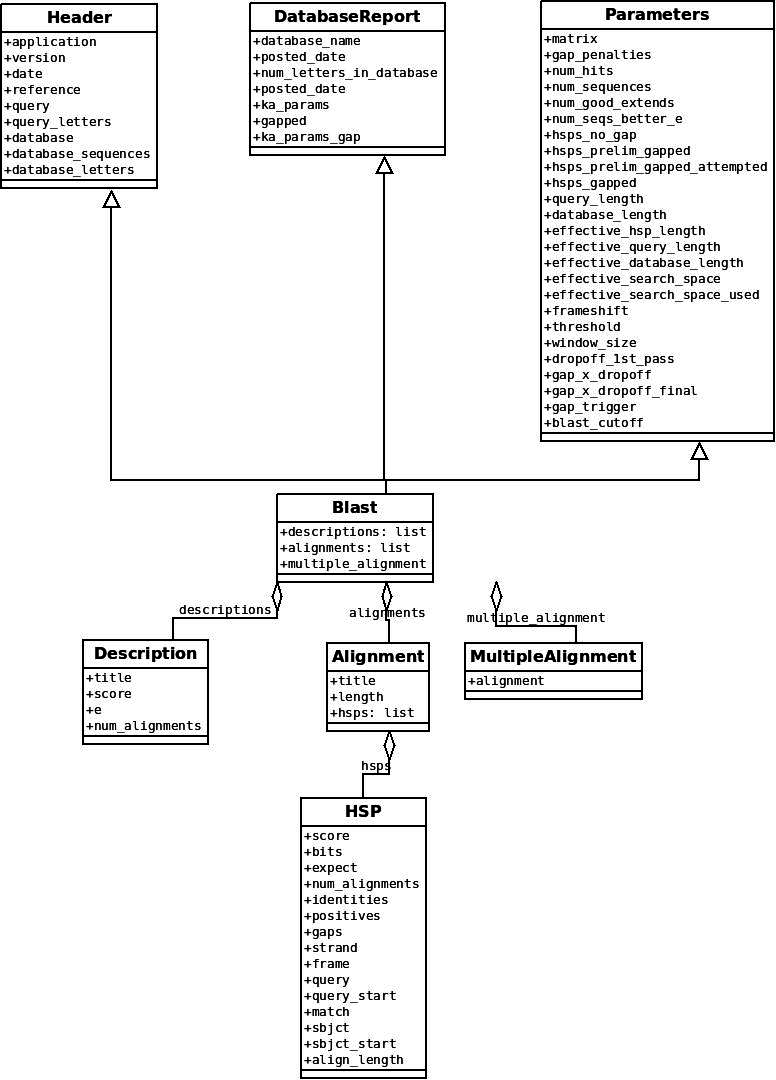
\includegraphics[width=0.8\textwidth]{images/BlastRecord.png}
\caption{Class diagram for the Blast Record class representing all of the info in a BLAST report}
\label{fig:blastrecord}
\end{figure}
\end{latexonly}

The PSIBlast record object is similar, but has support for the rounds that are used in the iteration steps of PSIBlast. The class diagram for PSIBlast is shown in Figure~\ref{fig:psiblastrecord}.

\begin{htmlonly}
\label{fig:psiblastrecord}
\imgsrc[width=650, height=750]{images/PSIBlastRecord.png}
\end{htmlonly}

\begin{latexonly}
\begin{figure}[htbp]
\centering
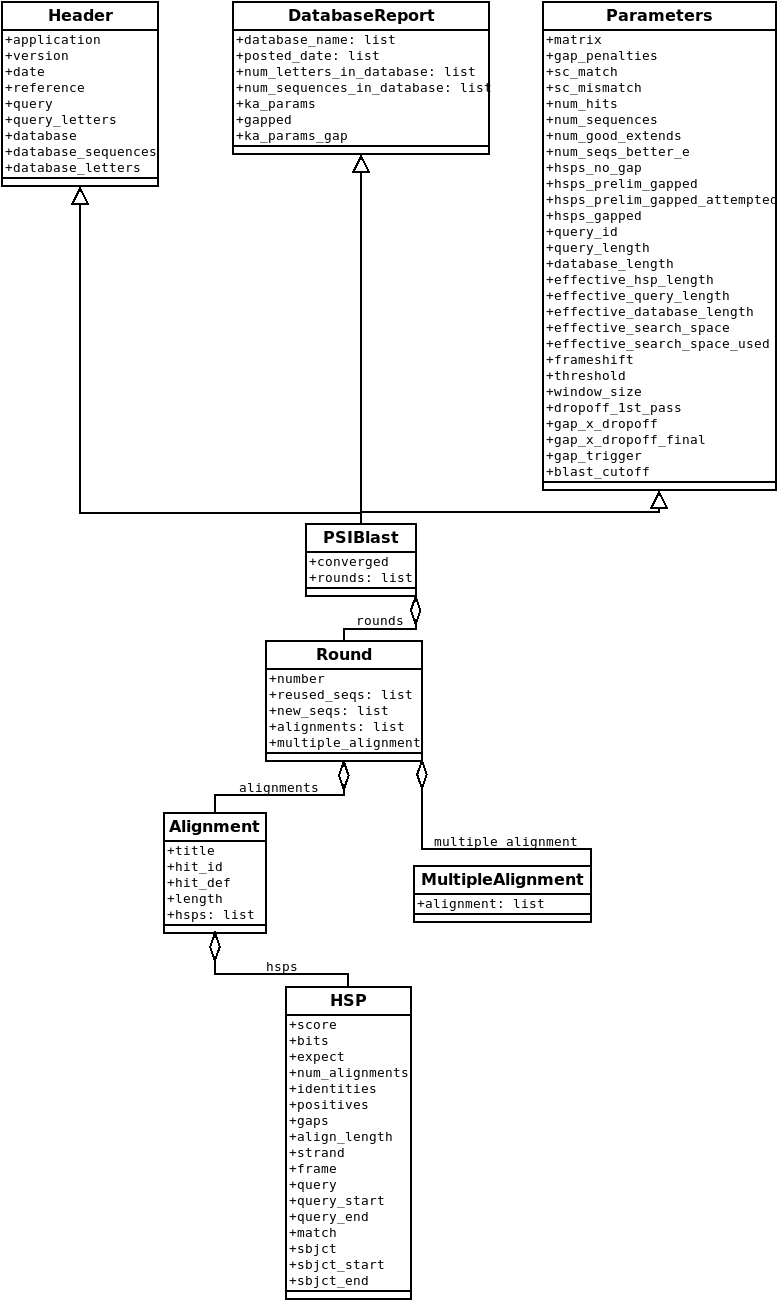
\includegraphics[width=0.8\textwidth]{images/PSIBlastRecord.png}
\caption{Class diagram for the PSIBlast Record class.}
\label{fig:psiblastrecord}
\end{figure}
\end{latexonly}

\section{Deprecated BLAST parsers}
\label{sec:parsing-blast-deprecated}

Older versions of Biopython had parsers for BLAST output in plain text or HTML
format. Over the years, we discovered that it is very hard to maintain these
parsers in working order. Basically, any small change to the BLAST output in
newly released BLAST versions tends to cause the plain text and HTML parsers
to break. We therefore recommend parsing BLAST output in XML format, as
described in section~\ref{sec:parsing-blast}.

Depending on which BLAST versions or programs you're using, our plain text BLAST parser may or may not work. Use it at your own risk!

\subsection{Parsing plain-text BLAST output}

The plain text BLAST parser is located in \verb|Bio.Blast.NCBIStandalone|.

As with the XML parser, we need to have a handle object that we can pass to the parser. The handle must implement the \verb|readline()| method and do this properly. The common ways to get such a handle are to either use the provided \verb|blastall| or \verb|blastpgp| functions to run the local blast, or to run a local blast via the command line, and then do something like the following:

\begin{verbatim}
>>> result_handle = open("my_file_of_blast_output.txt")
\end{verbatim}

Well, now that we've got a handle (which we'll call \verb|result_handle|),
we are ready to parse it. This can be done with the following code:

\begin{verbatim}
>>> from Bio.Blast import NCBIStandalone
>>> blast_parser = NCBIStandalone.BlastParser()
>>> blast_record = blast_parser.parse(result_handle)
\end{verbatim}

This will parse the BLAST report into a Blast Record class (either a Blast or a PSIBlast record, depending on what you are parsing) so that you can extract the information from it. In our case, let's just use print out a quick summary of all of the alignments greater than some threshold value.

\begin{verbatim}
>>> E_VALUE_THRESH = 0.04
>>> for alignment in blast_record.alignments:
...     for hsp in alignment.hsps:
...         if hsp.expect < E_VALUE_THRESH:
...             print '****Alignment****'
...             print 'sequence:', alignment.title
...             print 'length:', alignment.length
...             print 'e value:', hsp.expect
...             print hsp.query[0:75] + '...'
...             print hsp.match[0:75] + '...'
...             print hsp.sbjct[0:75] + '...'
\end{verbatim}

If you also read the section~\ref{sec:parsing-blast} on parsing BLAST XML output, you'll notice that the above code is identical to what is found in that section. Once you parse something into a record class you can deal with it independent of the format of the original BLAST info you were parsing. Pretty snazzy!

Sure, parsing one record is great, but I've got a BLAST file with tons of records -- how can I parse them all? Well, fear not, the answer lies in the very next section.

\subsection{Parsing a plain-text BLAST file full of BLAST runs}

We can do this using the blast iterator. To set up an iterator, we first set up a parser, to parse our blast reports in Blast Record objects:

\begin{verbatim}
>>> from Bio.Blast import NCBIStandalone
>>> blast_parser = NCBIStandalone.BlastParser()
\end{verbatim}

Then we will assume we have a handle to a bunch of blast records, which we'll call \verb|result_handle|. Getting a handle is described in full detail above in the blast parsing sections.

Now that we've got a parser and a handle, we are ready to set up the iterator with the following command:

\begin{verbatim}
>>> blast_iterator = NCBIStandalone.Iterator(result_handle, blast_parser)
\end{verbatim}

The second option, the parser, is optional. If we don't supply a parser, then the iterator will just return the raw BLAST reports one at a time.

Now that we've got an iterator, we start retrieving blast records (generated by our parser) using \verb|next()|:

\begin{verbatim}
>>> blast_record = blast_iterator.next()
\end{verbatim}

Each call to next will return a new record that we can deal with. Now we can iterate through this records and generate our old favorite, a nice little blast report:

\begin{verbatim}
>>> for blast_record in blast_iterator:
...     E_VALUE_THRESH = 0.04
...     for alignment in blast_record.alignments:
...         for hsp in alignment.hsps:
...             if hsp.expect < E_VALUE_THRESH:
...                 print '****Alignment****'
...                 print 'sequence:', alignment.title
...                 print 'length:', alignment.length
...                 print 'e value:', hsp.expect
...                 if len(hsp.query) > 75:
...                     dots = '...'
...                 else:
...                     dots = ''
...                 print hsp.query[0:75] + dots
...                 print hsp.match[0:75] + dots
...                 print hsp.sbjct[0:75] + dots
\end{verbatim}

%Notice that \verb|b_iterator.next()| will return \verb|None| when it runs out of records to parse, so it is easy to iterate through the entire file with a while loop that checks for the existence of a record.

The iterator allows you to deal with huge blast records without any memory problems, since things are read in one at a time. I have parsed tremendously huge files without any problems using this.

%TODO - Remove this or update it for BLAST XML parser
\subsection{Finding a bad record somewhere in a huge plain-text BLAST file}

One really ugly problem that happens to me is that I'll be parsing a huge blast file for a while, and the parser will bomb out with a ValueError. This is a serious problem, since you can't tell if the ValueError is due to a parser problem, or a problem with the BLAST. To make it even worse, you have no idea where the parse failed, so you can't just ignore the error, since this could be ignoring an important data point.

We used to have to make a little script to get around this problem, but the \verb|Bio.Blast| module now includes a \verb|BlastErrorParser| which really helps make this easier. The \verb|BlastErrorParser| works very similar to the regular \verb|BlastParser|, but it adds an extra layer of work by catching ValueErrors that are generated by the parser, and attempting to diagnose the errors.

Let's take a look at using this parser -- first we define the file we are going to parse and the file to write the problem reports to:

\begin{verbatim}
>>> import os
>>> blast_file = os.path.join(os.getcwd(), "blast_out", "big_blast.out")
>>> error_file = os.path.join(os.getcwd(), "blast_out", "big_blast.problems")
\end{verbatim}

Now we want to get a \verb|BlastErrorParser|:

\begin{verbatim}
>>> from Bio.Blast import NCBIStandalone
>>> error_handle = open(error_file, "w")
>>> blast_error_parser = NCBIStandalone.BlastErrorParser(error_handle)
\end{verbatim}

Notice that the parser take an optional argument of a handle. If a handle is passed, then the parser will write any blast records which generate a ValueError to this handle. Otherwise, these records will not be recorded.

Now we can use the \verb|BlastErrorParser| just like a regular blast parser. Specifically, we might want to make an iterator that goes through our blast records one at a time and parses them with the error parser:

\begin{verbatim}
>>> result_handle = open(blast_file)
>>> iterator = NCBIStandalone.Iterator(result_handle, blast_error_parser)
\end{verbatim}

We can read these records one a time, but now we can catch and deal with errors that are due to problems with Blast (and not with the parser itself):

\begin{verbatim}
>>> try:
...     next_record = iterator.next()
... except NCBIStandalone.LowQualityBlastError, info:
...     print "LowQualityBlastError detected in id %s" % info[1]
\end{verbatim}

The \verb|.next()| method is normally called indirectly via a \verb|for|-loop.
Right now the \verb|BlastErrorParser| can generate the following errors:

\begin{itemize}
  \item \verb|ValueError| -- This is the same error generated by the regular BlastParser, and is due to the parser not being able to parse a specific file. This is normally either due to a bug in the parser, or some kind of discrepancy between the version of BLAST you are using and the versions the parser is able to handle.

  \item \verb|LowQualityBlastError| -- When BLASTing a sequence that is of really bad quality (for example, a short sequence that is basically a stretch of one nucleotide), it seems that Blast ends up masking out the entire sequence and ending up with nothing to parse. In this case it will produce a truncated report that causes the parser to generate a ValueError. \verb|LowQualityBlastError| is reported in these cases. This error returns an info item with the following information:
  \begin{itemize}
    \item \verb|item[0]| -- The error message
    \item \verb|item[1]| -- The id of the input record that caused the error. This is really useful if you want to record all of the records that are causing problems.
  \end{itemize}
\end{itemize}

As mentioned, with each error generated, the BlastErrorParser will write the offending record to the specified \verb|error_handle|. You can then go ahead and look and these and deal with them as you see fit. Either you will be able to debug the parser with a single blast report, or will find out problems in your blast runs. Either way, it will definitely be a useful experience!

Hopefully the \verb|BlastErrorParser| will make it much easier to debug and deal with large Blast files.

\section{Dealing with PSI-BLAST}

You can run the standalone version of PSI-BLAST (the legacy NCBI command line
tool \verb|blastpgp|, or its replacement \verb|psiblast|) using the wrappers
in \verb|Bio.Blast.Applications| module.

At the time of writing, the NCBI do not appear to support tools running a
PSI-BLAST search via the internet.

Note that the \verb|Bio.Blast.NCBIXML| parser can read the XML output from
current versions of PSI-BLAST, but information like which sequences in each
iteration is new or reused isn't present in the XML file.
If you care about this information you may have more joy with the plain text
output and the \verb|PSIBlastParser| in \verb|Bio.Blast.NCBIStandalone|.

\section{Dealing with RPS-BLAST}

You can run the standalone version of RPS-BLAST (either the legacy NCBI
command line tool \verb|rpsblast|, or its replacement with the same name)
using the wrappers in \verb|Bio.Blast.Applications| module.

At the time of writing, the NCBI do not appear to support tools running an
RPS-BLAST search via the internet.

You can use the \verb|Bio.Blast.NCBIXML| parser to read the XML output from
current versions of RPS-BLAST.


\chapter{BLAST and other sequence search tools (\textit{experimental code})}
\label{chapter:searchio}

\emph{WARNING}: This chapter of the Tutorial describes an \emph{experimental}
module in Biopython. It is being included in Biopython and documented
here in  the tutorial in a pre-final state to allow a period of feedback
and refinement before we declare it stable. Until then the details will
probably change, and any scripts using the current \verb|Bio.SearchIO|
would need to be updated. Please keep this in mind! For stable code
working with NCBI BLAST, please continue to use Bio.Blast described
in the preceding Chapter~\ref{chapter:blast}.

Biological sequence identification is an integral part of bioinformatics.
Several tools are available for this, each with their own algorithms and
approaches, such as BLAST (arguably the most popular), FASTA, HMMER, and many
more. In general, these tools usually use your sequence to search a database of
potential matches. With the growing number of known sequences (hence the
growing number of potential matches), interpreting the results becomes
increasingly hard as there could be hundreds or even thousands of potential
matches. In this scenario, interpreting the results manually is out of the
question. Moreover, you often need to work with several sequence search tools,
each with its own statistics, conventions, and output format. Imagine how
daunting it would be when you need to work with multiple sequences using
multiple search tools.

We know this too well ourselves, which is why we created the \verb|Bio.SearchIO|
submodule in Biopython. \verb|Bio.SearchIO| allows you to extract information
from your search results in a convenient way, while also dealing with the
different standards and conventions used by different search tools.
The name \verb|SearchIO| is a homage to BioPerl's module of the same name.

In this chapter, we'll go through the main features of \verb|Bio.SearchIO| to
show what it can do for you. We'll use two popular search tools along the way:
BLAST and BLAT. They are used merely for illustrative purposes, and you should
be able to adapt the workflow to any other search tools supported by
\verb|Bio.SearchIO| in a breeze. You're very welcome to follow along with the
search output files we'll be using. The BLAST output file can be downloaded
here, and the BLAT output file here. Both output files were generated using
this sequence:
%TODO - Add the missing links above.

\begin{verbatim}
>mystery_seq
CCCTCTACAGGGAAGCGCTTTCTGTTGTCTGAAAGAAAAGAAAGTGCTTCCTTTTAGAGGG
\end{verbatim}

The BLAST result is an XML file generated using blastn against the NCBI
\verb|refseq_rna| database. For BLAT, the sequence database was the February 2009
\verb|hg19| human genome draft and the output format is PSL.

We'll start from an introduction to the \verb|Bio.SearchIO| object model. The
model is the representation of your search results, thus it is core to
\verb|Bio.SearchIO| itself. After that, we'll see the main methods in
\verb|Bio.SearchIO|, from the ones that reads in your search output files to
the ones that can write new files.

Now that we're all set let's go to the first step: introducing the core
object model.

\section{The SearchIO object model}
\label{sec:searchio-model}

Despite the wildly differing output styles among many sequence search tools,
it turns out that their underlying concept is similar:

\begin{itemize}
\item The output file may contain results from one or more search queries.
\item In each search query, you will see one or more hits from the given
search database.
\item In each database hit, you will see one or more regions containing the
actual sequence alignment between your query sequence and the database
sequence.
\item Some programs like BLAT or Exonerate may further split these regions into
several alignment fragments (or blocks in BLAT and possibly exons in
exonerate). This is not something you always see, as programs like BLAST and
HMMER do not do this.
\end{itemize}

Realizing this generality, we decided use it as base for creating the
\verb|Bio.SearchIO| object model. The object model consists of a nested
hierarchy of Python objects, each one representing one concept outlined above.
These objects are:

\begin{itemize}
\item \verb|QueryResult|, to represent a single search query.
\item \verb|Hit|, to represent a single database hit. \verb|Hit| objects are
    contained within \verb|QueryResult| and in each \verb|QueryResult| there is
    zero or more \verb|Hit| objects.
\item \verb|HSP| (short for high-scoring pair), to represent region(s) of
    significant alignments between query and hit sequences. \verb|HSP| objects
    are contained within \verb|Hit| objects and each \verb|Hit| has one or more
    \verb|HSP| objects.
\item \verb|HSPFragment|, to represent a single contiguous alignment between
    query and hit sequences. \verb|HSPFragment| objects are contained within
    \verb|HSP| objects. Most sequence search tools like BLAST and HMMER unify
    \verb|HSP| and \verb|HSPFragment| objects as each \verb|HSP| will only have
    a single \verb|HSPFragment|. However there are tools like BLAT and Exonerate
    that produce \verb|HSP| containing multiple \verb|HSPFragment|. Don't worry
    if this seems a tad confusing now, we'll elaborate more on these two objects
    later on.
\end{itemize}

These four objects are the ones you will interact with when you use
\verb|Bio.SearchIO|. They are created using one of the main \verb|Bio.SearchIO|
methods: \verb|read|, \verb|parse|, \verb|index|, or \verb|index_db|. The
details of these methods are provided in later sections. For this section, we'll
only be using read and parse so what you need to know is that read and parse
behave similarly to their \verb|Bio.SeqIO| and \verb|Bio.AlignIO| counterparts:

\begin{itemize}
\item \verb|read| is used for search output files with a single query and
    returns a \verb|QueryResult| object
\item \verb|parse| is used for search output files with multiple queries and
    returns a generator that yields \verb|QueryResult| objects
\end{itemize}

With that settled, let's start probing each \verb|Bio.SearchIO| object,
beginning with \verb|QueryResult|.

\subsection{QueryResult}
\label{sec:searchio-qresult}

The QueryResult object represents a single search query and contains zero or
more Hit objects. Let's see what it looks like using the BLAST file we have:

%doctest ../Tests/Tutorial
\begin{verbatim}
>>> from Bio import SearchIO
>>> blast_qresult = SearchIO.read('my_blast.xml', 'blast-xml')
>>> print blast_qresult
Program: blastn (2.2.27+)
  Query: 42291 (61)
         mystery_seq
 Target: refseq_rna
   Hits: ----  -----  ----------------------------------------------------------
            #  # HSP  ID + description                                          
         ----  -----  ----------------------------------------------------------
            0      1  gi|262205317|ref|NR_030195.1|  Homo sapiens microRNA 52...
            1      1  gi|301171311|ref|NR_035856.1|  Pan troglodytes microRNA...
            2      1  gi|270133242|ref|NR_032573.1|  Macaca mulatta microRNA ...
            3      2  gi|301171322|ref|NR_035857.1|  Pan troglodytes microRNA...
            4      1  gi|301171267|ref|NR_035851.1|  Pan troglodytes microRNA...
            5      2  gi|262205330|ref|NR_030198.1|  Homo sapiens microRNA 52...
            6      1  gi|262205302|ref|NR_030191.1|  Homo sapiens microRNA 51...
            7      1  gi|301171259|ref|NR_035850.1|  Pan troglodytes microRNA...
            8      1  gi|262205451|ref|NR_030222.1|  Homo sapiens microRNA 51...
            9      2  gi|301171447|ref|NR_035871.1|  Pan troglodytes microRNA...
           10      1  gi|301171276|ref|NR_035852.1|  Pan troglodytes microRNA...
           11      1  gi|262205290|ref|NR_030188.1|  Homo sapiens microRNA 51...
           12      1  gi|301171354|ref|NR_035860.1|  Pan troglodytes microRNA...
           13      1  gi|262205281|ref|NR_030186.1|  Homo sapiens microRNA 52...
           14      2  gi|262205298|ref|NR_030190.1|  Homo sapiens microRNA 52...
           15      1  gi|301171394|ref|NR_035865.1|  Pan troglodytes microRNA...
           16      1  gi|262205429|ref|NR_030218.1|  Homo sapiens microRNA 51...
           17      1  gi|262205423|ref|NR_030217.1|  Homo sapiens microRNA 52...
           18      1  gi|301171401|ref|NR_035866.1|  Pan troglodytes microRNA...
           19      1  gi|270133247|ref|NR_032574.1|  Macaca mulatta microRNA ...
           20      1  gi|262205309|ref|NR_030193.1|  Homo sapiens microRNA 52...
           21      2  gi|270132717|ref|NR_032716.1|  Macaca mulatta microRNA ...
           22      2  gi|301171437|ref|NR_035870.1|  Pan troglodytes microRNA...
           23      2  gi|270133306|ref|NR_032587.1|  Macaca mulatta microRNA ...
           24      2  gi|301171428|ref|NR_035869.1|  Pan troglodytes microRNA...
           25      1  gi|301171211|ref|NR_035845.1|  Pan troglodytes microRNA...
           26      2  gi|301171153|ref|NR_035838.1|  Pan troglodytes microRNA...
           27      2  gi|301171146|ref|NR_035837.1|  Pan troglodytes microRNA...
           28      2  gi|270133254|ref|NR_032575.1|  Macaca mulatta microRNA ...
           29      2  gi|262205445|ref|NR_030221.1|  Homo sapiens microRNA 51...
           ~~~
           97      1  gi|356517317|ref|XM_003527287.1|  PREDICTED: Glycine ma...
           98      1  gi|297814701|ref|XM_002875188.1|  Arabidopsis lyrata su...
           99      1  gi|397513516|ref|XM_003827011.1|  PREDICTED: Pan panisc...
\end{verbatim}

We've just begun to scratch the surface of the object model, but you can see that
there's already some useful information. By invoking \verb|print| on the
\verb|QueryResult| object, you can see:

\begin{itemize}
\item The program name and version (blastn version 2.2.27+)
\item The query ID, description, and its sequence length (ID is 42291,
    description is `mystery\_seq', and it is 61 nucleotides long)
\item The target database to search against (refseq\_rna)
\item A quick overview of the resulting hits. For our query sequence, there are
    100 potential hits (numbered 0--99 in the table). For each hit, we can also see
    how many HSPs it contains, its ID, and a snippet of its description. Notice
    here that \verb|Bio.SearchIO| truncates the hit table overview, by showing
    only hits numbered 0--29, and then 97--99.
\end{itemize}

Now let's check our BLAT results using the same procedure as above:

%cont-doctest
\begin{verbatim}
>>> blat_qresult = SearchIO.read('my_blat.psl', 'blat-psl')
>>> print blat_qresult
Program: blat (<unknown version>)
  Query: mystery_seq (61)
         <unknown description>
 Target: <unknown target>
   Hits: ----  -----  ----------------------------------------------------------
            #  # HSP  ID + description                                          
         ----  -----  ----------------------------------------------------------
            0     17  chr19  <unknown description>                              
\end{verbatim}

You'll immediately notice that there are some differences. Some of these are
caused by the way PSL format stores its details, as you'll see. The rest are
caused by the genuine program and target database differences between our BLAST
and BLAT searches:

\begin{itemize}
\item The program name and version. \verb|Bio.SearchIO| knows that the program
    is BLAT, but in the output file there is no information regarding the
    program version so it defaults to `<unknown version>'.
\item The query ID, description, and its sequence length. Notice here that these
    details is slightly different from the ones we see in BLAST. The ID is
    `mystery\_seq' instead of 42991, there is no known description, but the query
    length is still 61. This is actually a difference introduced by the file
    formats themselves. BLAST sometimes creates its own query IDs and uses your
    original ID as the sequence description.
\item The target database is not known, as it is not stated in the BLAT output
    file.
\item And finally, the list of hits we have is completely different. Here, we
    see that our query sequence only hits the `chr19' database entry, but in it
    we see 17 HSP regions. This should not be surprising however, given that we
    are using a different program on a different target database.
\end{itemize}

All the details you saw when invoking the \verb|print| method can be accessed
individually using Python's object attribute access notation (a.k.a. the dot
notation). There are also other format-specific attributes that you can access
using the same method.

%cont-doctest
\begin{verbatim}
>>> print "%s %s" % (blast_qresult.program, blast_qresult.version)
blastn 2.2.27+
>>> print "%s %s" % (blat_qresult.program, blat_qresult.version)
blat <unknown version>
>>> blast_qresult.param_evalue_threshold    # blast-xml specific
10.0
\end{verbatim}

For a complete list of accessible attributes, you can check each format-specific
documentation.

Having looked at using \verb|print| on \verb|QueryResult| objects, let's drill
down deeper. What exactly is a \verb|QueryResult|? In terms of Python objects,
\verb|QueryResult| is a hybrid between Python's built-in list and dictionary. In
other words, it is a container object with all the convenient features of lists
and dictionaries.

Like Python lists and dictionaries, \verb|QueryResult| objects are iterable.
Each iteration returns a \verb|Hit| object:

\begin{verbatim}
>>> for hit in blast_qresult:
...     hit
Hit(id='gi|262205317|ref|NR_030195.1|', query_id='42291', 1 hsps)
Hit(id='gi|301171311|ref|NR_035856.1|', query_id='42291', 1 hsps)
Hit(id='gi|270133242|ref|NR_032573.1|', query_id='42291', 1 hsps)
Hit(id='gi|301171322|ref|NR_035857.1|', query_id='42291', 2 hsps)
Hit(id='gi|301171267|ref|NR_035851.1|', query_id='42291', 1 hsps)
...
\end{verbatim}

To check how many items (hits) a \verb|QueryResult| has, you can simply invoke
Python's \verb|len| method:

%cont-doctest
\begin{verbatim}
>>> len(blast_qresult)
100
>>> len(blat_qresult)
1
\end{verbatim}

Like Python lists, you can retrieve items (hits) from a \verb|QueryResult| using
the slice notation:

%cont-doctest
\begin{verbatim}
>>> blast_qresult[0]        # retrieves the top hit
Hit(id='gi|262205317|ref|NR_030195.1|', query_id='42291', 1 hsps)
>>> blast_qresult[-1]       # retrieves the last hit
Hit(id='gi|397513516|ref|XM_003827011.1|', query_id='42291', 1 hsps)
\end{verbatim}

To retrieve multiple hits, you can slice \verb|QueryResult| objects using the
slice notation as well. In this case, the slice will return a new
\verb|QueryResult| object containing only the sliced hits:

%cont-doctest
\begin{verbatim}
>>> blast_slice = blast_qresult[:3]     # slices the first three hits
>>> print blast_slice
Program: blastn (2.2.27+)
  Query: 42291 (61)
         mystery_seq
 Target: refseq_rna
   Hits: ----  -----  ----------------------------------------------------------
            #  # HSP  ID + description                                          
         ----  -----  ----------------------------------------------------------
            0      1  gi|262205317|ref|NR_030195.1|  Homo sapiens microRNA 52...
            1      1  gi|301171311|ref|NR_035856.1|  Pan troglodytes microRNA...
            2      1  gi|270133242|ref|NR_032573.1|  Macaca mulatta microRNA ...
\end{verbatim}

Like Python dictionaries, you can also retrieve hits using the hit's ID. This is
particularly useful if you know a given hit ID exists within a search query
results:

%cont-doctest
\begin{verbatim}
>>> blast_qresult['gi|262205317|ref|NR_030195.1|']
Hit(id='gi|262205317|ref|NR_030195.1|', query_id='42291', 1 hsps)
\end{verbatim}

You can also get a full list of \verb|Hit| objects using \verb|hits| and a full
list of \verb|Hit| IDs using \verb|hit_keys|:

\begin{verbatim}
>>> blast_qresult.hits
[...]       # list of all hits
>>> blast_qresult.hit_keys
[...]       # list of all hit IDs
\end{verbatim}

What if you just want to check whether a particular hit is present in the query
results? You can do a simple Python membership test using the \verb|in| keyword:

%cont-doctest
\begin{verbatim}
>>> 'gi|262205317|ref|NR_030195.1|' in blast_qresult
True
>>> 'gi|262205317|ref|NR_030194.1|' in blast_qresult
False
\end{verbatim}

Sometimes, knowing whether a hit is present is not enough; you also want to know
the rank of the hit. Here, the \verb|index| method comes to the rescue:

%cont-doctest
\begin{verbatim}
>>> blast_qresult.index('gi|301171437|ref|NR_035870.1|')
22
\end{verbatim}

Remember that we're using Python's indexing style here, which is zero-based.
This means our hit above is ranked at no. 23, not 22.

Also, note that the hit rank you see here is based on the native hit ordering
present in the original search output file. Different search tools may have
order these hits based on different criteria.

If the native hit ordering doesn't suit your taste, you can use the \verb|sort|
method of the \verb|QueryResult| object. It is very similar to Python's
\verb|list.sort| method, with the addition of an option to create a new sorted
\verb|QueryResult| object or not.

Here is an example of using \verb|QueryResult.sort| to sort the hits based on
each hit's full sequence length. For this particular sort, we'll set the
\verb|in_place| flag to \verb|False| so that sorting will return a new
\verb|QueryResult| object and leave our initial object unsorted. We'll also set
the \verb|reverse| flag to \verb|True| so that we're doing a descending sort.

%cont-doctest
\begin{verbatim}
>>> for hit in blast_qresult[:5]:   # id and sequence length of the first five hits
...     print hit.id, hit.seq_len
...
gi|262205317|ref|NR_030195.1| 61
gi|301171311|ref|NR_035856.1| 60
gi|270133242|ref|NR_032573.1| 85
gi|301171322|ref|NR_035857.1| 86
gi|301171267|ref|NR_035851.1| 80

>>> sort_key = lambda hit: hit.seq_len
>>> sorted_qresult = blast_qresult.sort(key=sort_key, reverse=True, in_place=False)
>>> for hit in sorted_qresult[:5]:
...     print hit.id, hit.seq_len
...
gi|397513516|ref|XM_003827011.1| 6002
gi|390332045|ref|XM_776818.2| 4082
gi|390332043|ref|XM_003723358.1| 4079
gi|356517317|ref|XM_003527287.1| 3251
gi|356543101|ref|XM_003539954.1| 2936
\end{verbatim}

The advantage of having the \verb|in_place| flag here is that we're preserving
the native ordering, so we can come back to it later on in case we need it.
You should note that this is not the default behavior of
\verb|QueryResult.sort|, however, which is why we needed to set the flag to
\verb|True| explicitly.

At this point, you've known enough about \verb|QueryResult| objects to make it
work for you. But before we go on to the next object in the \verb|Bio.SearchIO|
model, let's take a look at two more sets of methods that could make it even
easier to work with \verb|QueryResult| objects: the \verb|filter| and \verb|map|
methods.

If you're familiar with Python's list comprehensions, generator expressions
or the built in \verb|filter| and \verb|map| functions,
you'll know how useful they are for working with list-like objects (if you're
not, check them out!). You can use these built in methods to manipulate
\verb|QueryResult| objects, but you'll end up with regular Python lists and lose
the ability to do more interesting manipulations.

That's why, \verb|QueryResult| objects provide its own flavor of
\verb|filter| and \verb|map| methods. Analogous to \verb|filter|, there are
\verb|hit_filter| and \verb|hsp_filter| methods. As their name implies, these
methods filter its \verb|QueryResult| object either on its \verb|Hit| objects
or \verb|HSP| objects. Similarly, analogous to \verb|map|, \verb|QueryResult|
objects also provide the \verb|hit_map| and \verb|hsp_map| methods. These
methods apply a given function to all hits or HSPs in a \verb|QueryResult|
object, respectively.

Let's see these methods in action, beginning with \verb|hit_filter|. This method
accepts a callback function that checks whether a given \verb|Hit| object passes
the condition you set or not. In other words, the function must accept as its
argument a single \verb|Hit| object and returns \verb|True| or \verb|False|.

Here is an example of using \verb|hit_filter| to filter out \verb|Hit| objects
that only have one HSP:

%cont-doctest
\begin{verbatim}
>>> filter_func = lambda hit: len(hit.hsps) > 1     # the callback function
>>> len(blast_qresult)      # no. of hits before filtering
100
>>> filtered_qresult = blast_qresult.hit_filter(filter_func)
>>> len(filtered_qresult)   # no. of hits after filtering
37
>>> for hit in filtered_qresult[:5]:    # quick check for the hit lengths
...     print hit.id, len(hit.hsps)
gi|301171322|ref|NR_035857.1| 2
gi|262205330|ref|NR_030198.1| 2
gi|301171447|ref|NR_035871.1| 2
gi|262205298|ref|NR_030190.1| 2
gi|270132717|ref|NR_032716.1| 2
\end{verbatim}

\verb|hsp_filter| works the same as \verb|hit_filter|, only instead of looking
at the \verb|Hit| objects, it performs filtering on the \verb|HSP| objects in
each hits.

As for the \verb|map| methods, they too accept a callback function as their
arguments. However, instead of returning \verb|True| or \verb|False|, the
callback function must return the modified \verb|Hit| or \verb|HSP| object
(depending on whether you're using \verb|hit_map| or \verb|hsp_map|).

Let's see an example where we're using \verb|hit_map| to rename the hit IDs:

%cont-doctest
\begin{verbatim}
>>> def map_func(hit):
...     hit.id = hit.id.split('|')[3]   # renames 'gi|301171322|ref|NR_035857.1|' to 'NR_035857.1'
...     return hit
...
>>> mapped_qresult = blast_qresult.hit_map(map_func)
>>> for hit in mapped_qresult[:5]:
...     print hit.id
NR_030195.1
NR_035856.1
NR_032573.1
NR_035857.1
NR_035851.1
\end{verbatim}

Again, \verb|hsp_map| works the same as \verb|hit_map|, but on \verb|HSP|
objects instead of \verb|Hit| objects.

\subsection{Hit}
\label{sec:searchio-hit}

\verb|Hit| objects represent all query results from a single database entry.
They are the second-level container in the \verb|Bio.SearchIO| object hierarchy.
You've seen that they are contained by \verb|QueryResult| objects, but they
themselves contain \verb|HSP| objects.

Let's see what they look like, beginning with our BLAST search:

%doctest ../Tests/Tutorial
\begin{verbatim}
>>> from Bio import SearchIO
>>> blast_qresult = SearchIO.read('my_blast.xml', 'blast-xml')
>>> blast_hit = blast_qresult[3]    # fourth hit from the query result
\end{verbatim}
%HACK: because Py2.5 in windows output floating points slightly different
\begin{verbatim}
>>> print blast_hit
Query: 42291
       mystery_seq
  Hit: gi|301171322|ref|NR_035857.1| (86)
       Pan troglodytes microRNA mir-520c (MIR520C), microRNA
 HSPs: ----  --------  ---------  ------  ---------------  ---------------------
          #   E-value  Bit score    Span      Query range              Hit range
       ----  --------  ---------  ------  ---------------  ---------------------
          0   8.9e-20     100.47      60           [1:61]                [13:73]
          1   3.3e-06      55.39      60           [0:60]                [13:73]
\end{verbatim}

You see that we've got the essentials covered here:

\begin{itemize}
\item The query ID and description is present. A hit is always tied to a query,
    so we want to keep track of the originating query as well. These values can
    be accessed from a hit using the \verb|query_id| and
    \verb|query_description| attributes.
\item We also have the unique hit ID, description, and full sequence lengths.
    They can be accessed using \verb|id|, \verb|description|, and
    \verb|seq_len|, respectively.
\item Finally, there's a table containing quick information about the HSPs this
    hit contains. In each row, we've got the important HSP details listed: the
    HSP index, its e-value, its bit score, its span (the alignment length
    including gaps), its query coordinates, and its hit coordinates.
\end{itemize}

Now let's contrast this with the BLAT search. Remember that in the BLAT search we
had one hit with 17 HSPs.

%cont-doctest
\begin{verbatim}
>>> blat_qresult = SearchIO.read('my_blat.psl', 'blat-psl')
>>> blat_hit = blat_qresult[0]      # the only hit
>>> print blat_hit
Query: mystery_seq
       <unknown description>
  Hit: chr19 (59128983)
       <unknown description>
 HSPs: ----  --------  ---------  ------  ---------------  ---------------------
          #   E-value  Bit score    Span      Query range              Hit range
       ----  --------  ---------  ------  ---------------  ---------------------
          0         ?          ?       ?           [0:61]    [54204480:54204541]
          1         ?          ?       ?           [0:61]    [54233104:54264463]
          2         ?          ?       ?           [0:61]    [54254477:54260071]
          3         ?          ?       ?           [1:61]    [54210720:54210780]
          4         ?          ?       ?           [0:60]    [54198476:54198536]
          5         ?          ?       ?           [0:61]    [54265610:54265671]
          6         ?          ?       ?           [0:61]    [54238143:54240175]
          7         ?          ?       ?           [0:60]    [54189735:54189795]
          8         ?          ?       ?           [0:61]    [54185425:54185486]
          9         ?          ?       ?           [0:60]    [54197657:54197717]
         10         ?          ?       ?           [0:61]    [54255662:54255723]
         11         ?          ?       ?           [0:61]    [54201651:54201712]
         12         ?          ?       ?           [8:60]    [54206009:54206061]
         13         ?          ?       ?          [10:61]    [54178987:54179038]
         14         ?          ?       ?           [8:61]    [54212018:54212071]
         15         ?          ?       ?           [8:51]    [54234278:54234321]
         16         ?          ?       ?           [8:61]    [54238143:54238196]
\end{verbatim}

Here, we've got a similar level of detail as with the BLAST hit we saw earlier.
There are some differences worth explaining, though:

\begin{itemize}
\item The e-value and bit score column values. As BLAT HSPs do not have e-values
    and bit scores, the display defaults to `?'.
\item What about the span column? The span values is meant to display the
    complete alignment length, which consists of all residues and any gaps that
    may be present. The PSL format do not have this information readily available
    and \verb|Bio.SearchIO| does not attempt to try guess what it is, so we get a
    `?' similar to the e-value and bit score columns.
\end{itemize}

In terms of Python objects, \verb|Hit| behaves almost the same as Python lists,
but contain \verb|HSP| objects exclusively. If you're familiar with lists, you
should encounter no difficulties working with the \verb|Hit| object. 

Just like Python lists, \verb|Hit| objects are iterable, and each iteration
returns one \verb|HSP| object it contains:

%cont-doctest
\begin{verbatim}
>>> for hsp in blast_hit:
...     hsp
HSP(hit_id='gi|301171322|ref|NR_035857.1|', query_id='42291', 1 fragments)
HSP(hit_id='gi|301171322|ref|NR_035857.1|', query_id='42291', 1 fragments)
\end{verbatim}

You can invoke \verb|len| on a \verb|Hit| to see how many \verb|HSP| objects it
has:

%cont-doctest
\begin{verbatim}
>>> len(blast_hit)
2
>>> len(blat_hit)
17
\end{verbatim}

You can use the slice notation on \verb|Hit| objects, whether to retrieve single
\verb|HSP| or multiple \verb|HSP| objects. Like \verb|QueryResult|, if you slice
for multiple \verb|HSP|, a new \verb|Hit| object will be returned containing
only the sliced \verb|HSP| objects:

%cont-doctest
\begin{verbatim}
>>> blat_hit[0]                 # retrieve single items
HSP(hit_id='chr19', query_id='mystery_seq', 1 fragments)
>>> sliced_hit = blat_hit[4:9]  # retrieve multiple items
>>> len(sliced_hit)
5
>>> print sliced_hit
Query: mystery_seq
       <unknown description>
  Hit: chr19 (59128983)
       <unknown description>
 HSPs: ----  --------  ---------  ------  ---------------  ---------------------
          #   E-value  Bit score    Span      Query range              Hit range
       ----  --------  ---------  ------  ---------------  ---------------------
          0         ?          ?       ?           [0:60]    [54198476:54198536]
          1         ?          ?       ?           [0:61]    [54265610:54265671]
          2         ?          ?       ?           [0:61]    [54238143:54240175]
          3         ?          ?       ?           [0:60]    [54189735:54189795]
          4         ?          ?       ?           [0:61]    [54185425:54185486]
\end{verbatim}

You can also sort the \verb|HSP| inside a \verb|Hit|, using the exact same
arguments like the sort method you saw in the \verb|QueryResult| object.

And finally, there are also the \verb|filter| and \verb|map| methods you can use
on \verb|Hit| objects. Unlike in the \verb|QueryResult| object, \verb|Hit|
objects only have one variant of \verb|filter| (\verb|Hit.filter|) and one
variant of \verb|map| (\verb|Hit.map|). Both of \verb|Hit.filter| and
\verb|Hit.map| work on the \verb|HSP| objects a \verb|Hit| has.

\subsection{HSP}
\label{sec:searchio-hsp}

\verb|HSP| (high-scoring pair) represents region(s) in the hit sequence that
contains significant alignment(s) to the query sequence. It contains the actual
match between your query sequence and a database entry. As this match is
determined by the sequence search tool's algorithms, the \verb|HSP| object
contains the bulk of the statistics computed by the search tool. This also makes
the distinction between \verb|HSP| objects from different search tools more
apparent compared to the differences you've seen in \verb|QueryResult| or
\verb|Hit| objects.

Let's see some examples from our BLAST and BLAT searches. We'll look at the
BLAST HSP first:

%doctest ../Tests/Tutorial
\begin{verbatim}
>>> from Bio import SearchIO
>>> blast_qresult = SearchIO.read('my_blast.xml', 'blast-xml')
>>> blast_hsp = blast_qresult[0][0]    # first hit, first hsp
\end{verbatim}
%HACK: because Py2.5 in windows output floating points slightly different
\begin{verbatim}
>>> print blast_hsp
      Query: 42291 mystery_seq
        Hit: gi|262205317|ref|NR_030195.1| Homo sapiens microRNA 520b (MIR520...
Query range: [0:61] (1)
  Hit range: [0:61] (1)
Quick stats: evalue 4.9e-23; bitscore 111.29
  Fragments: 1 (61 columns)
     Query - CCCTCTACAGGGAAGCGCTTTCTGTTGTCTGAAAGAAAAGAAAGTGCTTCCTTTTAGAGGG
             |||||||||||||||||||||||||||||||||||||||||||||||||||||||||||||
       Hit - CCCTCTACAGGGAAGCGCTTTCTGTTGTCTGAAAGAAAAGAAAGTGCTTCCTTTTAGAGGG
\end{verbatim}

Just like \verb|QueryResult| and \verb|Hit|, invoking \verb|print| on an
\verb|HSP| shows its general details:
\begin{itemize}
\item There are the query and hit IDs and descriptions. We need these to
    identify our \verb|HSP|.
\item We've also got the matching range of the query and hit sequences. The
    slice notation we're using here is an indication that the range is displayed
    using Python's indexing style (zero-based, half open). The number inside the
    parenthesis denotes the strand. In this case, both sequences have the plus
    strand.
\item Some quick statistics are available: the e-value and bitscore.
\item There is information about the HSP fragments. Ignore this for now; it will
    be explained later on.
\item And finally, we have the query and hit sequence alignment itself.
\end{itemize}

These details can be accessed on their own using the dot notation, just like in
\verb|QueryResult| and \verb|Hit|:

%cont-doctest
\begin{verbatim}
>>> blast_hsp.query_range
(0, 61)
\end{verbatim}
%hack! since float display may be different across versions
\begin{verbatim}
>>> blast_hsp.evalue
4.91307e-23
\end{verbatim}

They're not the only attributes available, though. \verb|HSP| objects come with
a default set of properties that makes it easy to probe for their various
details. Here are some examples:

%cont-doctest
\begin{verbatim}
>>> blast_hsp.hit_start         # start coordinate of the hit sequence
0
>>> blast_hsp.query_span        # how many residues in the query sequence
61
>>> blast_hsp.aln_span          # how long the alignment is
61
\end{verbatim}

Check out the \verb|HSP| documentation for a full list of these predefined
properties.

Furthermore, each sequence search tool usually computes its own statistics /
details for its \verb|HSP| objects. For example, an XML BLAST search also
outputs the number of gaps and identical residues. These attributes can be
accessed like so:

%cont-doctest
\begin{verbatim}
>>> blast_hsp.gap_num       # number of gaps
0
>>> blast_hsp.ident_num     # number of identical residues
61
\end{verbatim}

These details are format-specific; they may not be present in other formats.
To see which details are available for a given sequence search tool, you
should check the format's documentation in \verb|Bio.SearchIO|. Alternatively,
you may also use \verb|.__dict__.keys()| for a quick list of what's available:

\begin{verbatim}
>>> blast_hsp.__dict__.keys()
['bitscore', 'evalue', 'ident_num', 'gap_num', 'bitscore_raw', 'pos_num', '_items']
\end{verbatim}

Finally, you may have noticed that the \verb|query| and \verb|hit| attributes
of our HSP are not just regular strings:

%cont-doctest
\begin{verbatim}
>>> blast_hsp.query
SeqRecord(seq=Seq('CCCTCTACAGGGAAGCGCTTTCTGTTGTCTGAAAGAAAAGAAAGTGCTTCCTTT...GGG', DNAAlphabet()), id='42291', name='aligned query sequence', description='mystery_seq', dbxrefs=[])
>>> blast_hsp.hit
SeqRecord(seq=Seq('CCCTCTACAGGGAAGCGCTTTCTGTTGTCTGAAAGAAAAGAAAGTGCTTCCTTT...GGG', DNAAlphabet()), id='gi|262205317|ref|NR_030195.1|', name='aligned hit sequence', description='Homo sapiens microRNA 520b (MIR520B), microRNA', dbxrefs=[])
\end{verbatim}

They are \verb|SeqRecord| objects you saw earlier in
Section~\ref{chapter:SeqRecord}! This means that you can do all sorts of
interesting things you can do with \verb|SeqRecord| objects on \verb|HSP.query|
and/or \verb|HSP.hit|. 

It probably should not surprise you that the \verb|HSP| object has an
\verb|alignment| property made up by the \verb|MultipleSeqAlignment| object:

%cont-doctest
\begin{verbatim}
>>> print blast_hsp.aln
DNAAlphabet() alignment with 2 rows and 61 columns
CCCTCTACAGGGAAGCGCTTTCTGTTGTCTGAAAGAAAAGAAAG...GGG 42291
CCCTCTACAGGGAAGCGCTTTCTGTTGTCTGAAAGAAAAGAAAG...GGG gi|262205317|ref|NR_030195.1|
\end{verbatim}

Having probed the BLAST HSP, let's now take a look at HSPs from our BLAT
results for a different kind of HSP. As usual, we'll begin by invoking
\verb|print| on it:

%cont-doctest
\begin{verbatim}
>>> blat_qresult = SearchIO.read('my_blat.psl', 'blat-psl')
>>> blat_hsp = blat_qresult[0][0]       # first hit, first hsp
>>> print blat_hsp
      Query: mystery_seq <unknown description>
        Hit: chr19 <unknown description>
Query range: [0:61] (1)
  Hit range: [54204480:54204541] (1)
Quick stats: evalue ?; bitscore ?
  Fragments: 1 (? columns)
\end{verbatim}

Some of the outputs you may have already guessed. We have the query and hit IDs
and descriptions and the sequence coordinates. Values for evalue and bitscore is
`?' as BLAT HSPs do not have these attributes. But The biggest difference here
is that you don't see any sequence alignments displayed. If you look closer, PSL
formats themselves do not have any hit or query sequences, so
\verb|Bio.SearchIO| won't create any sequence or alignment objects. What happens
if you try to access \verb|HSP.query|, \verb|HSP.hit|, or \verb|HSP.aln|?
You'll get the default values for these attributes, which is \verb|None|:

%cont-doctest
\begin{verbatim}
>>> blat_hsp.hit is None
True
>>> blat_hsp.query is None
True
>>> blat_hsp.aln is None
True
\end{verbatim}

This does not affect other attributes, though. For example, you can still
access the length of the query or hit alignment. Despite not displaying any
attributes, the PSL format still have this information so \verb|Bio.SearchIO|
can extract them:

%cont-doctest
\begin{verbatim}
>>> blat_hsp.query_span     # length of query match
61
>>> blat_hsp.hit_span       # length of hit match
61
\end{verbatim}

Other format-specific attributes are still present as well:

%cont-doctest
\begin{verbatim}
>>> blat_hsp.score          # PSL score
61
>>> blat_hsp.mismatch_num   # the mismatch column
0
\end{verbatim}

So far so good? Things get more interesting when you look at another `variant'
of HSP present in our BLAT results. You might recall that in BLAT searches,
sometimes we get our results separated into `blocks'. These blocks are
essentially alignment fragments that may have some intervening sequence between
them.

Let's take a look at a BLAT HSP that contains multiple blocks to see how
\verb|Bio.SearchIO| deals with this:

%cont-doctest
\begin{verbatim}
>>> blat_hsp2 = blat_qresult[0][1]      # first hit, second hsp
>>> print blat_hsp2
      Query: mystery_seq <unknown description>
        Hit: chr19 <unknown description>
Query range: [0:61] (1)
  Hit range: [54233104:54264463] (1)
Quick stats: evalue ?; bitscore ?
  Fragments: ---  --------------  ----------------------  ----------------------
               #            Span             Query range               Hit range
             ---  --------------  ----------------------  ----------------------
               0               ?                  [0:18]     [54233104:54233122]
               1               ?                 [18:61]     [54264420:54264463]
\end{verbatim}

What's happening here? We still some essential details covered: the IDs and
descriptions, the coordinates, and the quick statistics are similar to what
you've seen before. But the fragments detail is all different. Instead of
showing `Fragments: 1', we now have a table with two data rows.

This is how \verb|Bio.SearchIO| deals with HSPs having multiple fragments. As
mentioned before, an HSP alignment may be separated by intervening sequences
into fragments. The intervening sequences are not part of the query-hit match,
so they should not be considered part of query nor hit sequence. However, they
do affect how we deal with sequence coordinates, so we can't ignore them.

Take a look at the hit coordinate of the HSP above. In the \verb|Hit range:| field,
we see that the coordinate is \verb|[54233104:54264463]|. But looking at the
table rows, we see that not the entire region spanned by this coordinate matches
our query. Specifically, the intervening region spans from \verb|54233122| to
\verb|54264420|.

Why then, is the query coordinates seem to be contiguous, you ask? This is
perfectly fine. In this case it means that the query match is contiguous (no
intervening regions), while the hit match is not.

All these attributes are accessible from the HSP directly, by the way:

%cont-doctest
\begin{verbatim}
>>> blat_hsp2.hit_range         # hit start and end coordinates of the entire HSP
(54233104, 54264463)
>>> blat_hsp2.hit_range_all     # hit start and end coordinates of each fragment
[(54233104, 54233122), (54264420, 54264463)]
>>> blat_hsp2.hit_span          # hit span of the entire HSP
31359
>>> blat_hsp2.hit_span_all      # hit span of each fragment
[18, 43]
>>> blat_hsp2.hit_inter_ranges  # start and end coordinates of intervening regions in the hit sequence
[(54233122, 54264420)]
>>> blat_hsp2.hit_inter_spans   # span of intervening regions in the hit sequence
[31298]
\end{verbatim}

Most of these attributes are not readily available from the PSL file we have,
but \verb|Bio.SearchIO| calculates them for you on the fly when you ask for
them. All it needs are the start and end coordinates of each fragment.

What about the \verb|query|, \verb|hit|, and \verb|aln| attributes? If the
HSP has multiple fragments, you won't be able to use these attributes as they
only fetch single \verb|SeqRecord| or \verb|MultipleSeqAlignment| objects.
However, you can use their \verb|*_all| counterparts: \verb|query_all|,
\verb|hit_all|, and \verb|aln_all|. These properties will return a list containing
\verb|SeqRecord| or \verb|MultipleSeqAlignment| objects from each of the HSP
fragment. There are other attributes that behave similarly, i.e. they only work
for HSPs with one fragment. Check out the \verb|HSP| documentation for a full
list.

Finally, to check whether you have multiple fragments or not, you can use the
\verb|is_fragmented| property like so:

%cont-doctest
\begin{verbatim}
>>> blat_hsp2.is_fragmented     # BLAT HSP with 2 fragments
True
>>> blat_hsp.is_fragmented      # BLAT HSP from earlier, with one fragment
False
\end{verbatim}

Before we move on, you should also know that we can use the slice notation on
\verb|HSP| objects, just like \verb|QueryResult| or \verb|Hit| objects. When
you use this notation, you'll get an \verb|HSPFragment| object in return, the
last component of the object model.

\subsection{HSPFragment}
\label{sec:searchio-hspfragment}

\verb|HSPFragment| represents a single, contiguous match between the query and
hit sequences. You could consider it the core of the object model and search
result, since it is the presence of these fragments that determine whether your
search have results or not.

In most cases, you don't have to deal with \verb|HSPFragment| objects directly
since not that many sequence search tools fragment their HSPs. When you do have
to deal with them, what you should remember is that \verb|HSPFragment| objects
were written with simplicity in mind. In most cases, they only contain
attributes directly related to sequences: strands, reading frames, alphabets,
coordinates, the sequences themselves, and their IDs and descriptions.

These attributes are readily shown when you invoke \verb|print| on an
\verb|HSPFragment|. Here's an example, taken from our BLAST search:

%doctest ../Tests/Tutorial
\begin{verbatim}
>>> from Bio import SearchIO
>>> blast_qresult = SearchIO.read('my_blast.xml', 'blast-xml')
>>> blast_frag = blast_qresult[0][0][0]    # first hit, first hsp, first fragment
>>> print blast_frag
      Query: 42291 mystery_seq
        Hit: gi|262205317|ref|NR_030195.1| Homo sapiens microRNA 520b (MIR520...
Query range: [0:61] (1)
  Hit range: [0:61] (1)
  Fragments: 1 (61 columns)
     Query - CCCTCTACAGGGAAGCGCTTTCTGTTGTCTGAAAGAAAAGAAAGTGCTTCCTTTTAGAGGG
             |||||||||||||||||||||||||||||||||||||||||||||||||||||||||||||
       Hit - CCCTCTACAGGGAAGCGCTTTCTGTTGTCTGAAAGAAAAGAAAGTGCTTCCTTTTAGAGGG
\end{verbatim}

At this level, the BLAT fragment looks quite similar to the BLAST fragment, save
for the query and hit sequences which are not present:

%cont-doctest
\begin{verbatim}
>>> blat_qresult = SearchIO.read('my_blat.psl', 'blat-psl')
>>> blat_frag = blat_qresult[0][0][0]    # first hit, first hsp, first fragment
>>> print blat_frag
      Query: mystery_seq <unknown description>
        Hit: chr19 <unknown description>
Query range: [0:61] (1)
  Hit range: [54204480:54204541] (1)
  Fragments: 1 (? columns)
\end{verbatim}

In all cases, these attributes are accessible using our favorite dot notation.
Some examples:

%cont-doctest
\begin{verbatim}
>>> blast_frag.query_start      # query start coordinate
0
>>> blast_frag.hit_strand       # hit sequence strand
1
>>> blast_frag.hit              # hit sequence, as a SeqRecord object
SeqRecord(seq=Seq('CCCTCTACAGGGAAGCGCTTTCTGTTGTCTGAAAGAAAAGAAAGTGCTTCCTTT...GGG', DNAAlphabet()), id='gi|262205317|ref|NR_030195.1|', name='aligned hit sequence', description='Homo sapiens microRNA 520b (MIR520B), microRNA', dbxrefs=[])
\end{verbatim}

\section{A note about standards and conventions}
\label{sec:searchio-standards}

Before we move on to the main functions, there is something you ought to know
about the standards \verb|Bio.SearchIO| uses. If you've worked with multiple
sequence search tools, you might have had to deal with the many different ways
each program deals with things like sequence coordinates. It might not have been
a pleasant experience as these search tools usually have their own standards.
For example, one tools might use one-based coordinates, while the other uses
zero-based coordinates. Or, one program might reverse the start and end
coordinates if the strand is minus, while others don't. In short, these often
creates unnecessary mess that we must deal with.

We realize this problem ourselves and we intend to address it in
\verb|Bio.SearchIO|. After all, one of the goals of \verb|Bio.SearchIO| is to
create a common, easy to use interface to deal with various search output files.
This means creating standards that extend beyond the object model you just saw.

Now, you might complain, "Not another standard!". Well, eventually we have to
choose one convention or the other, so this is necessary. Plus, we're not
creating something entirely new here; just adopting a standard we think is best
for a Python programmer (it is Biopython, after all).

There are three implicit standards that you can expect when working with
\verb|Bio.SearchIO|:

\begin{itemize}
\item The first one pertains to sequence coordinates. In \verb|Bio.SearchIO|,
    all sequence coordinates follows Python's coordinate style: zero-based and
    half open. For example, if in a BLAST XML output file the start and end
    coordinates of an HSP are 10 and 28, they would become 9 and 28 in
    \verb|Bio.SearchIO|. The start coordinate becomes 9 because Python indices
    start from zero, while the end coordinate remains 28 as Python slices omit
    the last item in an interval.
\item The second is on sequence coordinate orders. In \verb|Bio.SearchIO|, start
    coordinates are always less than or equal to end coordinates. This isn't
    always the case with all sequence search tools, as some of them have larger
    start coordinates when the sequence strand is minus.
\item The last one is on strand and reading frame values. For strands, there are
    only four valid choices: \verb|1| (plus strand), \verb|-1| (minus strand),
    \verb|0| (protein sequences), and \verb|None| (no strand). For reading
    frames, the valid choices are integers from \verb|-3| to \verb|3| and
    \verb|None|.
\end{itemize}

Note that these standards only exist in \verb|Bio.SearchIO| objects. If you
write \verb|Bio.SearchIO| objects into an output format, \verb|Bio.SearchIO|
will use the format's standard for the output. It does not force its standard
over to your output file.

\section{Reading search output files}
\label{sec:searchio-input}

There are two functions you can use for reading search output files into
\verb|Bio.SearchIO| objects: \verb|read| and \verb|parse|. They're essentially
similar to \verb|read| and \verb|parse| functions in other submodules like
\verb|Bio.SeqIO| or \verb|Bio.AlignIO|. In both cases, you need to supply the
search output file name and the file format name, both as Python strings. You
can check the documentation for a list of format names \verb|Bio.SearchIO|
recognizes.

\verb|Bio.SearchIO.read| is used for reading search output files with only one
query and returns a \verb|QueryResult| object. You've seen \verb|read| used in
our previous examples. What you haven't seen is that \verb|read| may also accept
additional keyword arguments, depending on the file format.

Here are some examples. In the first one, we use \verb|read| just like
previously to read a BLAST tabular output file. In the second one, we use a
keyword argument to modify so it parses the BLAST tabular variant with comments
in it:

%doctest ../Tests/Blast
\begin{verbatim}
>>> from Bio import SearchIO
>>> qresult = SearchIO.read('tab_2226_tblastn_003.txt', 'blast-tab')
>>> qresult
QueryResult(id='gi|16080617|ref|NP_391444.1|', 3 hits)
>>> qresult2 = SearchIO.read('tab_2226_tblastn_007.txt', 'blast-tab', comments=True)
>>> qresult2
QueryResult(id='gi|16080617|ref|NP_391444.1|', 3 hits)
\end{verbatim}

These keyword arguments differs among file formats. Check the format
documentation to see if it has keyword arguments that modifies its parser's
behavior.

As for the \verb|Bio.SearchIO.parse|, it is used for reading search output
files with any number of queries. The function returns a generator object that
yields a \verb|QueryResult| object in each iteration. Like
\verb|Bio.SearchIO.read|, it also accepts format-specific keyword arguments:

%doctest ../Tests/Blast
\begin{verbatim}
>>> from Bio import SearchIO
>>> qresults = SearchIO.parse('tab_2226_tblastn_001.txt', 'blast-tab')
>>> for qresult in qresults:
...     print qresult.id
gi|16080617|ref|NP_391444.1|
gi|11464971:4-101
>>> qresults2 = SearchIO.parse('tab_2226_tblastn_005.txt', 'blast-tab', comments=True)
>>> for qresult in qresults2:
...     print qresult.id
random_s00
gi|16080617|ref|NP_391444.1|
gi|11464971:4-101
\end{verbatim}

\section{Dealing with large search output files with indexing}
\label{sec:searchio-index}

Sometimes, you're handed a search output file containing hundreds or thousands
of queries that you need to parse. You can of course use
\verb|Bio.SearchIO.parse| for this file, but that would be grossly inefficient
if you need to access only a few of the queries. This is because \verb|parse|
will parse all queries it sees before it reaches the query you want.

In this case, the ideal choice would be to index the file using
\verb|Bio.SearchIO.index| or \verb|Bio.SearchIO.index_db|. If the names sound
familiar it's because you've seen them before in  Section~\ref{sec:SeqIO-index}.
These functions also behave similarly to their \verb|Bio.SeqIO| counterparts,
with the addition of format-specific keyword arguments.

Here are some examples. You can use \verb|index| with just the filename and
format name:

%doctest ../Tests/Blast
\begin{verbatim}
>>> from Bio import SearchIO
>>> idx = SearchIO.index('tab_2226_tblastn_001.txt', 'blast-tab')
>>> sorted(idx.keys())
['gi|11464971:4-101', 'gi|16080617|ref|NP_391444.1|']
>>> idx['gi|16080617|ref|NP_391444.1|']
QueryResult(id='gi|16080617|ref|NP_391444.1|', 3 hits)
\end{verbatim}

Or also with the format-specific keyword argument:

%cont-doctest
\begin{verbatim}
>>> idx = SearchIO.index('tab_2226_tblastn_005.txt', 'blast-tab', comments=True)
>>> sorted(idx.keys())
['gi|11464971:4-101', 'gi|16080617|ref|NP_391444.1|', 'random_s00']
>>> idx['gi|16080617|ref|NP_391444.1|']
QueryResult(id='gi|16080617|ref|NP_391444.1|', 3 hits)
\end{verbatim}

Or with the \verb|key_function| argument, as in \verb|Bio.SeqIO|:

%cont-doctest
\begin{verbatim}
>>> key_function = lambda id: id.upper()    # capitalizes the keys
>>> idx = SearchIO.index('tab_2226_tblastn_001.txt', 'blast-tab', key_function=key_function)
>>> sorted(idx.keys())
['GI|11464971:4-101', 'GI|16080617|REF|NP_391444.1|']
>>> idx['GI|16080617|REF|NP_391444.1|']
QueryResult(id='gi|16080617|ref|NP_391444.1|', 3 hits)
\end{verbatim}

\verb|Bio.SearchIO.index_db| works like as \verb|index|, only it writes the
query offsets into an SQLite database file.

\section{Writing and converting search output files}
\label{sec:searchio-write}

It is occasionally useful to be able to manipulate search results from an output
file and write it again to a new file. \verb|Bio.SearchIO| provides a
\verb|write| function that lets you do exactly this. It takes as its arguments
an iterable returning \verb|QueryResult| objects, the output filename to write
to, the format name to write to, and optionally some format-specific keyword
arguments. It returns a four-item tuple, which denotes the number or
\verb|QueryResult|, \verb|Hit|, \verb|HSP|, and \verb|HSPFragment| objects that
were written.

\begin{verbatim}
>>> from Bio import SearchIO
>>> qresults = SearchIO.parse('mirna.xml', 'blast-xml')     # read XML file
>>> SearchIO.write(qresults, 'results.tab', 'blast-tab')    # write to tabular file
(3, 239, 277, 277)
\end{verbatim}

You should note different file formats require different attributes of the
\verb|QueryResult|, \verb|Hit|, \verb|HSP| and \verb|HSPFragment| objects. If
these attributes are not present, writing won't work. In other words, you can't
always write to the output format that you want. For example, if you read a
BLAST XML file, you wouldn't be able to write the results to a PSL file as PSL
files require attributes not calculated by BLAST (e.g. the number of repeat
matches). You can always set these attributes manually, if you really want to
write to PSL, though.

Like \verb|read|, \verb|parse|, \verb|index|, and \verb|index_db|, \verb|write|
also accepts format-specific keyword arguments. Check out the documentation for
a complete list of formats \verb|Bio.SearchIO| can write to and their arguments.

Finally, \verb|Bio.SearchIO| also provides a \verb|convert| function, which is
simply a shortcut for \verb|Bio.SearchIO.parse| and \verb|Bio.SearchIO.write|.
Using the convert function, our example above would be:

\begin{verbatim}
>>> from Bio import SearchIO
>>> SearchIO.convert('mirna.xml', 'blast-xml', 'results.tab', 'blast-tab')
(3, 239, 277, 277)
\end{verbatim}

As \verb|convert| uses \verb|write|, it is only limited to format conversions
that have all the required attributes. Here, the BLAST XML file provides all the
default values a BLAST tabular file requires, so it works just fine. However,
other format conversions are less likely to work since you need to manually
assign the required attributes first.

\chapter{Accessing NCBI's Entrez databases}
\label{chapter:entrez}

Entrez (\url{http://www.ncbi.nlm.nih.gov/Entrez}) is a data retrieval system that provides users access to NCBI's databases such as PubMed, GenBank, GEO, and many others. You can access Entrez from a web browser to manually enter queries, or you can use Biopython's \verb+Bio.Entrez+ module for programmatic access to Entrez. The latter allows you for example to search PubMed or download GenBank records from within a Python script.

The \verb+Bio.Entrez+ module makes use of the Entrez Programming Utilities (also known as EUtils), consisting of eight tools that are described in detail on NCBI's page at \url{http://www.ncbi.nlm.nih.gov/entrez/utils/}.
Each of these tools corresponds to one Python function in the \verb+Bio.Entrez+ module, as described in the sections below. This module makes sure that the correct URL is used for the queries, and that not more than one request is made every three seconds, as required by NCBI.

The output returned by the Entrez Programming Utilities is typically in XML format. To parse such output, you have several options:
\begin{enumerate}
  \item Use \verb+Bio.Entrez+'s parser to parse the XML output into a Python object;
  \item Use the DOM (Document Object Model) parser in Python's standard library;
  \item Use the SAX (Simple API for XML) parser in Python's standard library;
  \item Read the XML output as raw text, and parse it by string searching and manipulation.
\end{enumerate}
For the DOM and SAX parsers, see the Python documentation. The parser in \verb+Bio.Entrez+ is discussed below.

NCBI uses DTD (Document Type Definition) files to describe the structure of the information contained in XML files. Most of the DTD files used by NCBI are included in the Biopython distribution. The \verb+Bio.Entrez+ parser makes use of the DTD files when parsing an XML file returned by NCBI Entrez.

Occasionally, you may find that the DTD file associated with a specific XML file is missing in the Biopython distribution. In particular, this may happen when NCBI updates its DTD files. If this happens, \verb+Entrez.read+ will show a warning message with the name and URL of the missing DTD file. The parser will proceed to access the missing DTD file through the internet, allowing the parsing of the XML file to continue.  However, the parser is much faster if the DTD file is available locally. For this purpose, please download the DTD file from the URL in the warning message and place it in the directory \verb+...site-packages/Bio/Entrez/DTDs+, containing the other DTD files.  If you don't have write access to this directory, you can also place the DTD file in \verb+~/.biopython/Bio/Entrez/DTDs+, where \verb+~+ represents your home directory. Since this directory is read before the directory \verb+...site-packages/Bio/Entrez/DTDs+, you can also put newer versions of DTD files there if the ones in \verb+...site-packages/Bio/Entrez/DTDs+ become outdated. Alternatively, if you installed Biopython from source, you can add the DTD file to the source code's \verb+Bio/Entrez/DTDs+ directory, and reinstall Biopython. This will install the new DTD file in the correct location together with the other DTD files.

The Entrez Programming Utilities can also generate output in other formats, such as the Fasta or GenBank file formats for sequence databases, or the MedLine format for the literature database, discussed in Section~\ref{sec:entrez-specialized-parsers}.

\section{Entrez Guidelines}
\label{sec:entrez-guidelines}
Before using Biopython to access the NCBI's online resources (via \verb|Bio.Entrez| or some of the other modules), please read the
\href{http://www.ncbi.nlm.nih.gov/books/NBK25497/#chapter2.Usage_Guidelines_and_Requiremen}{NCBI's Entrez User Requirements}.
If the NCBI finds you are abusing their systems, they can and will ban your access! 

To paraphrase:

\begin{itemize}
\item For any series of more than 100 requests, do this at weekends or outside USA peak times.  This is up to you to obey.
\item Use the \url{http://eutils.ncbi.nlm.nih.gov} address, not the standard NCBI Web address.  Biopython uses this web address.
\item Make no more than three requests every seconds (relaxed from at most one request every three seconds in early 2009).  This is automatically enforced by Biopython.
\item Use the optional email parameter so the NCBI can contact you if there is a problem.  You can either explicitly set this as a parameter with each call to Entrez (e.g. include {\tt email="A.N.Other@example.com"} in the argument list), or as of Biopython 1.48, you can set a global email address:
\begin{verbatim}
>>> from Bio import Entrez
>>> Entrez.email = "A.N.Other@example.com"
\end{verbatim}
{\tt Bio.Entrez} will then use this email address with each call to Entrez.  The {\tt example.com} address is a reserved domain name specifically for documentation (RFC 2606).  Please DO NOT use a random email -- it's better not to give an email at all. The email parameter will be mandatory from June 1, 2010. In case of excessive usage, NCBI will attempt to contact a user at the e-mail address provided prior to blocking access to the E-utilities.
\item If you are using Biopython within some larger software suite, use the tool parameter to specify this.  You can either explicitly set the tool name as a parameter with each call to Entrez (e.g. include {\tt tool="MyLocalScript"} in the argument list), or as of Biopython 1.54, you can set a global tool name:
\begin{verbatim}
>>> from Bio import Entrez
>>> Entrez.tool = "MyLocalScript"
\end{verbatim}
The tool parameter will default to Biopython.
\item For large queries, the NCBI also recommend using their session history feature (the WebEnv session cookie string, see Section~\ref{sec:entrez-webenv}).  This is only slightly more complicated.
\end{itemize}

In conclusion, be sensible with your usage levels.  If you plan to download lots of data, consider other options.  For example, if you want easy access to all the human genes, consider fetching each chromosome by FTP as a GenBank file, and importing these into your own BioSQL database (see Section~\ref{sec:BioSQL}).

\section{EInfo: Obtaining information about the Entrez databases}
\label{sec:entrez-einfo}
EInfo provides field index term counts, last update, and available links for each of NCBI's databases. In addition, you can use EInfo to obtain a list of all database names accessible through the Entrez utilities:
\begin{verbatim}
>>> from Bio import Entrez
>>> Entrez.email = "A.N.Other@example.com"     # Always tell NCBI who you are
>>> handle = Entrez.einfo()
>>> result = handle.read()
\end{verbatim}
The variable \verb+result+ now contains a list of databases in XML format:
\begin{verbatim}
>>> print result
<?xml version="1.0"?>
<!DOCTYPE eInfoResult PUBLIC "-//NLM//DTD eInfoResult, 11 May 2002//EN"
 "http://www.ncbi.nlm.nih.gov/entrez/query/DTD/eInfo_020511.dtd">
<eInfoResult>
<DbList>
        <DbName>pubmed</DbName>
        <DbName>protein</DbName>
        <DbName>nucleotide</DbName>
        <DbName>nuccore</DbName>
        <DbName>nucgss</DbName>
        <DbName>nucest</DbName>
        <DbName>structure</DbName>
        <DbName>genome</DbName>
        <DbName>books</DbName>
        <DbName>cancerchromosomes</DbName>
        <DbName>cdd</DbName>
        <DbName>gap</DbName>
        <DbName>domains</DbName>
        <DbName>gene</DbName>
        <DbName>genomeprj</DbName>
        <DbName>gensat</DbName>
        <DbName>geo</DbName>
        <DbName>gds</DbName>
        <DbName>homologene</DbName>
        <DbName>journals</DbName>
        <DbName>mesh</DbName>
        <DbName>ncbisearch</DbName>
        <DbName>nlmcatalog</DbName>
        <DbName>omia</DbName>
        <DbName>omim</DbName>
        <DbName>pmc</DbName>
        <DbName>popset</DbName>
        <DbName>probe</DbName>
        <DbName>proteinclusters</DbName>
        <DbName>pcassay</DbName>
        <DbName>pccompound</DbName>
        <DbName>pcsubstance</DbName>
        <DbName>snp</DbName>
        <DbName>taxonomy</DbName>
        <DbName>toolkit</DbName>
        <DbName>unigene</DbName>
        <DbName>unists</DbName>
</DbList>
</eInfoResult>
\end{verbatim}

Since this is a fairly simple XML file, we could extract the information it contains simply by string searching. Using \verb+Bio.Entrez+'s parser instead, we can directly parse this XML file into a Python object:
\begin{verbatim}
>>> from Bio import Entrez
>>> handle = Entrez.einfo()
>>> record = Entrez.read(handle)
\end{verbatim}
Now \verb+record+ is a dictionary with exactly one key:
\begin{verbatim}
>>> record.keys()
[u'DbList']
\end{verbatim}
The values stored in this key is the list of database names shown in the XML above:
\begin{verbatim}
>>> record["DbList"]
['pubmed', 'protein', 'nucleotide', 'nuccore', 'nucgss', 'nucest',
 'structure', 'genome', 'books', 'cancerchromosomes', 'cdd', 'gap',
 'domains', 'gene', 'genomeprj', 'gensat', 'geo', 'gds', 'homologene',
 'journals', 'mesh', 'ncbisearch', 'nlmcatalog', 'omia', 'omim', 'pmc',
 'popset', 'probe', 'proteinclusters', 'pcassay', 'pccompound',
 'pcsubstance', 'snp', 'taxonomy', 'toolkit', 'unigene', 'unists']
\end{verbatim}

For each of these databases, we can use EInfo again to obtain more information:
\begin{verbatim}
>>> handle = Entrez.einfo(db="pubmed")
>>> record = Entrez.read(handle)
>>> record["DbInfo"]["Description"]
'PubMed bibliographic record'
>>> record["DbInfo"]["Count"]
'17989604'
>>> record["DbInfo"]["LastUpdate"]
'2008/05/24 06:45'
\end{verbatim}
Try \verb+record["DbInfo"].keys()+ for other information stored in this record.
One of the most useful is a list of possible search fields for use with ESearch:

\begin{verbatim}
>>> for field in record["DbInfo"]["FieldList"]:
...     print "%(Name)s, %(FullName)s, %(Description)s" % field
ALL, All Fields, All terms from all searchable fields
UID, UID, Unique number assigned to publication
FILT, Filter, Limits the records
TITL, Title, Words in title of publication
WORD, Text Word, Free text associated with publication
MESH, MeSH Terms, Medical Subject Headings assigned to publication
MAJR, MeSH Major Topic, MeSH terms of major importance to publication
AUTH, Author, Author(s) of publication
JOUR, Journal, Journal abbreviation of publication
AFFL, Affiliation, Author's institutional affiliation and address
...
\end{verbatim}

That's a long list, but indirectly this tells you that for the PubMed
database, you can do things like \texttt{Jones[AUTH]} to search the
author field, or \texttt{Sanger[AFFL]} to restrict to authors at the
Sanger Centre. This can be very handy - especially if you are not so
familiar with a particular database.

\section{ESearch: Searching the Entrez databases}
\label{sec:entrez-esearch}
To search any of these databases, we use \verb+Bio.Entrez.esearch()+. For example, let's search in PubMed for publications related to Biopython:
\begin{verbatim}
>>> from Bio import Entrez
>>> Entrez.email = "A.N.Other@example.com"     # Always tell NCBI who you are
>>> handle = Entrez.esearch(db="pubmed", term="biopython")
>>> record = Entrez.read(handle)
>>> record["IdList"]
['19304878', '18606172', '16403221', '16377612', '14871861', '14630660', '12230038']
\end{verbatim}
In this output, you see seven PubMed IDs (including 19304878 which is the PMID for the Biopython application note), which can be retrieved by EFetch (see section \ref{sec:efetch}).

You can also use ESearch to search GenBank. Here we'll do a quick
search for the \emph{matK} gene in \emph{Cypripedioideae} orchids
(see Section~\ref{sec:entrez-einfo} about EInfo for one way to
find out which fields you can search in each Entrez database):

\begin{verbatim}
>>> handle = Entrez.esearch(db="nucleotide",term="Cypripedioideae[Orgn] AND matK[Gene]")
>>> record = Entrez.read(handle)
>>> record["Count"]
'25'
>>> record["IdList"]
['126789333', '37222967', '37222966', '37222965', ..., '61585492']
\end{verbatim}

\noindent Each of the IDs (126789333, 37222967, 37222966, \ldots) is a GenBank identifier.
See section~\ref{sec:efetch} for information on how to actually download these GenBank records.

Note that instead of a species name like \texttt{Cypripedioideae[Orgn]}, you can restrict the search using an NCBI taxon identifier, here this would be \texttt{txid158330[Orgn]}.  This isn't currently documented on the ESearch help page - the NCBI explained this in reply to an email query.  You can often deduce the search term formatting by playing with the Entrez web interface.  For example, including \texttt{complete[prop]} in a genome search restricts to just completed genomes.

As a final example, let's get a list of computational journal titles:
\begin{verbatim}
>>> handle = Entrez.esearch(db="journals", term="computational")
>>> record = Entrez.read(handle)
>>> record["Count"]
'16'
>>> record["IdList"]
['30367', '33843', '33823', '32989', '33190', '33009', '31986',
 '34502', '8799', '22857', '32675', '20258', '33859', '32534',
 '32357', '32249']
\end{verbatim}
Again, we could use EFetch to obtain more information for each of these journal IDs.

ESearch has many useful options --- see the \href{http://www.ncbi.nlm.nih.gov/entrez/query/static/esearch\_help.html}{ESearch help page} for more information.

\section{EPost: Uploading a list of identifiers}
EPost uploads a list of UIs for use in subsequent search strategies; see the
\href{http://www.ncbi.nlm.nih.gov/entrez/query/static/epost\_help.html}{EPost help page} for more information. It is available from Biopython through
the \verb+Bio.Entrez.epost()+ function.

To give an example of when this is useful, suppose you have a long list of IDs
you want to download using EFetch (maybe sequences, maybe citations --
anything). When you make a  request with EFetch your list of IDs, the database
etc, are all turned into a long URL sent to the server.  If your list of IDs is
long, this URL gets long, and long URLs can break (e.g. some proxies don't
cope well).

Instead, you can break this up into two steps, first uploading the list of IDs
using EPost (this uses an ``HTML post'' internally, rather than an ``HTML get'',
getting round the long URL problem).  With the history support, you can then
refer to this long list of IDs, and download the associated data with EFetch.

Let's look at a simple example to see how EPost works -- uploading some PubMed identifiers:
\begin{verbatim}
>>> from Bio import Entrez
>>> Entrez.email = "A.N.Other@example.com"     # Always tell NCBI who you are
>>> id_list = ["19304878", "18606172", "16403221", "16377612", "14871861", "14630660"]
>>> print Entrez.epost("pubmed", id=",".join(id_list)).read()
<?xml version="1.0"?>
<!DOCTYPE ePostResult PUBLIC "-//NLM//DTD ePostResult, 11 May 2002//EN"
 "http://www.ncbi.nlm.nih.gov/entrez/query/DTD/ePost_020511.dtd">
<ePostResult>
	<QueryKey>1</QueryKey>
	<WebEnv>NCID_01_206841095_130.14.22.101_9001_1242061629</WebEnv>
</ePostResult>
\end{verbatim}
\noindent The returned XML includes two important strings, \verb|QueryKey| and \verb|WebEnv| which together define your history session.
You would extract these values for use with another Entrez call such as EFetch:
\begin{verbatim}
>>> from Bio import Entrez
>>> Entrez.email = "A.N.Other@example.com"     # Always tell NCBI who you are
>>> id_list = ["19304878", "18606172", "16403221", "16377612", "14871861", "14630660"]
>>> search_results = Entrez.read(Entrez.epost("pubmed", id=",".join(id_list)))
>>> webenv = search_results["WebEnv"]
>>> query_key = search_results["QueryKey"] 
\end{verbatim}
\noindent Section~\ref{sec:entrez-webenv} shows how to use the history feature.

\section{ESummary: Retrieving summaries from primary IDs}
ESummary retrieves document summaries from a list of primary IDs (see the  \href{http://www.ncbi.nlm.nih.gov/entrez/query/static/esummary\_help.html}{ESummary help page} for more information). In Biopython, ESummary is available as \verb+Bio.Entrez.esummary()+. Using the search result above, we can for example find out more about the journal with ID 30367:
\begin{verbatim}
>>> from Bio import Entrez
>>> Entrez.email = "A.N.Other@example.com"     # Always tell NCBI who you are
>>> handle = Entrez.esummary(db="journals", id="30367")
>>> record = Entrez.read(handle)
>>> record[0]["Id"]
'30367'
>>> record[0]["Title"]
'Computational biology and chemistry'
>>> record[0]["Publisher"]
'Pergamon,'
\end{verbatim}

\section{EFetch: Downloading full records from Entrez}
\label{sec:efetch}

EFetch is what you use when you want to retrieve a full record from Entrez.
This covers several possible databases, as described on the main \href{http://eutils.ncbi.nlm.nih.gov/entrez/query/static/efetch_help.html}{EFetch Help page}.

For most of their databases, the NCBI support several different file formats. Requesting a specific file format from Entrez using \verb|Bio.Entrez.efetch()| requires specifying the \verb|rettype| and/or \verb|retmode| optional arguments.  The different combinations are described for each database type on the pages linked to on \href{http://www.ncbi.nlm.nih.gov/entrez/query/static/efetch_help.html}{NCBI efetch webpage} (e.g. \href{http://eutils.ncbi.nlm.nih.gov/corehtml/query/static/efetchlit_help.html}{literature}, \href{http://eutils.ncbi.nlm.nih.gov/corehtml/query/static/efetchseq_help.html}{sequences} and \href{http://eutils.ncbi.nlm.nih.gov/corehtml/query/static/efetchtax_help.html}{taxonomy}).

One common usage is downloading sequences in the FASTA or GenBank/GenPept plain text formats (which can then be parsed with \verb|Bio.SeqIO|, see Sections~\ref{sec:SeqIO_GenBank_Online} and~\ref{sec:efetch}). From the \emph{Cypripedioideae} example above, we can download GenBank record 186972394 using \verb+Bio.Entrez.efetch+:

\begin{verbatim}
>>> from Bio import Entrez
>>> Entrez.email = "A.N.Other@example.com"     # Always tell NCBI who you are
>>> handle = Entrez.efetch(db="nucleotide", id="186972394", rettype="gb", retmode="text")
>>> print handle.read()
LOCUS       EU490707                1302 bp    DNA     linear   PLN 05-MAY-2008
DEFINITION  Selenipedium aequinoctiale maturase K (matK) gene, partial cds;
            chloroplast.
ACCESSION   EU490707
VERSION     EU490707.1  GI:186972394
KEYWORDS    .
SOURCE      chloroplast Selenipedium aequinoctiale
  ORGANISM  Selenipedium aequinoctiale
            Eukaryota; Viridiplantae; Streptophyta; Embryophyta; Tracheophyta;
            Spermatophyta; Magnoliophyta; Liliopsida; Asparagales; Orchidaceae;
            Cypripedioideae; Selenipedium.
REFERENCE   1  (bases 1 to 1302)
  AUTHORS   Neubig,K.M., Whitten,W.M., Carlsward,B.S., Blanco,M.A.,
            Endara,C.L., Williams,N.H. and Moore,M.J.
  TITLE     Phylogenetic utility of ycf1 in orchids
  JOURNAL   Unpublished
REFERENCE   2  (bases 1 to 1302)
  AUTHORS   Neubig,K.M., Whitten,W.M., Carlsward,B.S., Blanco,M.A.,
            Endara,C.L., Williams,N.H. and Moore,M.J.
  TITLE     Direct Submission
  JOURNAL   Submitted (14-FEB-2008) Department of Botany, University of
            Florida, 220 Bartram Hall, Gainesville, FL 32611-8526, USA
FEATURES             Location/Qualifiers
     source          1..1302
                     /organism="Selenipedium aequinoctiale"
                     /organelle="plastid:chloroplast"
                     /mol_type="genomic DNA"
                     /specimen_voucher="FLAS:Blanco 2475"
                     /db_xref="taxon:256374"
     gene            <1..>1302
                     /gene="matK"
     CDS             <1..>1302
                     /gene="matK"
                     /codon_start=1
                     /transl_table=11
                     /product="maturase K"
                     /protein_id="ACC99456.1"
                     /db_xref="GI:186972395"
                     /translation="IFYEPVEIFGYDNKSSLVLVKRLITRMYQQNFLISSVNDSNQKG
                     FWGHKHFFSSHFSSQMVSEGFGVILEIPFSSQLVSSLEEKKIPKYQNLRSIHSIFPFL
                     EDKFLHLNYVSDLLIPHPIHLEILVQILQCRIKDVPSLHLLRLLFHEYHNLNSLITSK
                     KFIYAFSKRKKRFLWLLYNSYVYECEYLFQFLRKQSSYLRSTSSGVFLERTHLYVKIE
                     HLLVVCCNSFQRILCFLKDPFMHYVRYQGKAILASKGTLILMKKWKFHLVNFWQSYFH
                     FWSQPYRIHIKQLSNYSFSFLGYFSSVLENHLVVRNQMLENSFIINLLTKKFDTIAPV
                     ISLIGSLSKAQFCTVLGHPISKPIWTDFSDSDILDRFCRICRNLCRYHSGSSKKQVLY
                     RIKYILRLSCARTLARKHKSTVRTFMRRLGSGLLEEFFMEEE"
ORIGIN      
        1 attttttacg aacctgtgga aatttttggt tatgacaata aatctagttt agtacttgtg
       61 aaacgtttaa ttactcgaat gtatcaacag aattttttga tttcttcggt taatgattct
      121 aaccaaaaag gattttgggg gcacaagcat tttttttctt ctcatttttc ttctcaaatg
      181 gtatcagaag gttttggagt cattctggaa attccattct cgtcgcaatt agtatcttct
      241 cttgaagaaa aaaaaatacc aaaatatcag aatttacgat ctattcattc aatatttccc
      301 tttttagaag acaaattttt acatttgaat tatgtgtcag atctactaat accccatccc
      361 atccatctgg aaatcttggt tcaaatcctt caatgccgga tcaaggatgt tccttctttg
      421 catttattgc gattgctttt ccacgaatat cataatttga atagtctcat tacttcaaag
      481 aaattcattt acgccttttc aaaaagaaag aaaagattcc tttggttact atataattct
      541 tatgtatatg aatgcgaata tctattccag tttcttcgta aacagtcttc ttatttacga
      601 tcaacatctt ctggagtctt tcttgagcga acacatttat atgtaaaaat agaacatctt
      661 ctagtagtgt gttgtaattc ttttcagagg atcctatgct ttctcaagga tcctttcatg
      721 cattatgttc gatatcaagg aaaagcaatt ctggcttcaa agggaactct tattctgatg
      781 aagaaatgga aatttcatct tgtgaatttt tggcaatctt attttcactt ttggtctcaa
      841 ccgtatagga ttcatataaa gcaattatcc aactattcct tctcttttct ggggtatttt
      901 tcaagtgtac tagaaaatca tttggtagta agaaatcaaa tgctagagaa ttcatttata
      961 ataaatcttc tgactaagaa attcgatacc atagccccag ttatttctct tattggatca
     1021 ttgtcgaaag ctcaattttg tactgtattg ggtcatccta ttagtaaacc gatctggacc
     1081 gatttctcgg attctgatat tcttgatcga ttttgccgga tatgtagaaa tctttgtcgt
     1141 tatcacagcg gatcctcaaa aaaacaggtt ttgtatcgta taaaatatat acttcgactt
     1201 tcgtgtgcta gaactttggc acggaaacat aaaagtacag tacgcacttt tatgcgaaga
     1261 ttaggttcgg gattattaga agaattcttt atggaagaag aa
//
\end{verbatim}

The arguments \verb+rettype="gb"+ and \verb+retmode="text"+ let us download this record in the GenBank format.

Note that until Easter 2009, the Entrez EFetch API let you use ``genbank'' as the
return type, however the NCBI now insist on using the official return types of
``gb'' or ``gbwithparts'' (or ``gp'' for proteins) as described on online.
Also not that until Feb 2012, the Entrez EFetch API would default to returning
plain text files, but now defaults to XML.

Alternatively, you could for example use \verb+rettype="fasta"+ to get the Fasta-format; see the \href{http://www.ncbi.nlm.nih.gov/entrez/query/static/efetchseq\_help.html}{EFetch Sequences Help page} for other options. Remember -- the available formats depend on which database you are downloading from - see the main \href{http://eutils.ncbi.nlm.nih.gov/entrez/query/static/efetch\_help.html}{EFetch Help page}.

If you fetch the record in one of the formats accepted by \verb+Bio.SeqIO+ (see Chapter~\ref{chapter:Bio.SeqIO}), you could directly parse it into a \verb+SeqRecord+:

\begin{verbatim}
>>> from Bio import Entrez, SeqIO
>>> handle = Entrez.efetch(db="nucleotide", id="186972394",rettype="gb", retmode="text")
>>> record = SeqIO.read(handle, "genbank")
>>> handle.close()
>>> print record
ID: EU490707.1
Name: EU490707
Description: Selenipedium aequinoctiale maturase K (matK) gene, partial cds; chloroplast.
Number of features: 3
...
Seq('ATTTTTTACGAACCTGTGGAAATTTTTGGTTATGACAATAAATCTAGTTTAGTA...GAA', IUPACAmbiguousDNA())
\end{verbatim}

Note that a more typical use would be to save the sequence data to a local file, and \emph{then} parse it with \verb|Bio.SeqIO|.  This can save you having to re-download the same file repeatedly while working on your script, and places less load on the NCBI's servers.  For example:

\begin{verbatim}
import os
from Bio import SeqIO
from Bio import Entrez
Entrez.email = "A.N.Other@example.com"     # Always tell NCBI who you are
filename = "gi_186972394.gbk"
if not os.path.isfile(filename):
    # Downloading...
    net_handle = Entrez.efetch(db="nucleotide",id="186972394",rettype="gb", retmode="text")
    out_handle = open(filename, "w")
    out_handle.write(net_handle.read())
    out_handle.close()
    net_handle.close()
    print "Saved"

print "Parsing..."
record = SeqIO.read(filename, "genbank")
print record
\end{verbatim}

To get the output in XML format, which you can parse using the \verb+Bio.Entrez.read()+ function, use \verb+retmode="xml"+:

\begin{verbatim}
>>> from Bio import Entrez
>>> handle = Entrez.efetch(db="nucleotide", id="186972394", retmode="xml")
>>> record = Entrez.read(handle)
>>> handle.close()
>>> record[0]["GBSeq_definition"] 
'Selenipedium aequinoctiale maturase K (matK) gene, partial cds; chloroplast'
>>> record[0]["GBSeq_source"] 
'chloroplast Selenipedium aequinoctiale'
\end{verbatim}

So, that dealt with sequences. For examples of parsing file formats specific to the other databases (e.g. the \verb+MEDLINE+ format used in PubMed), see Section~\ref{sec:entrez-specialized-parsers}.

If you want to perform a search with \verb|Bio.Entrez.esearch()|, and then download the records with \verb|Bio.Entrez.efetch()|, you should use the WebEnv history feature -- see Section~\ref{sec:entrez-webenv}.

\section{ELink: Searching for related items in NCBI Entrez}
\label{sec:elink}

ELink, available from Biopython as \verb+Bio.Entrez.elink()+, can be used to find related items in the NCBI Entrez databases. For example, you can us this to find nucleotide entries for an entry in the gene database,
and other cool stuff.

Let's use ELink to find articles related to the Biopython application note published in \textit{Bioinformatics} in 2009. The PubMed ID of this article is 19304878:

\begin{verbatim}
>>> from Bio import Entrez
>>> Entrez.email = "A.N.Other@example.com"
>>> pmid = "19304878"
>>> record = Entrez.read(Entrez.elink(dbfrom="pubmed", id=pmid))
\end{verbatim}

The \verb+record+ variable consists of a Python list, one for each database in which we searched. Since we specified only one PubMed ID to search for, \verb+record+ contains only one item. This item is a dictionary containing information about our search term, as well as all the related items that were found:

\begin{verbatim}
>>> record[0]["DbFrom"]
'pubmed'
>>> record[0]["IdList"]
['19304878']
\end{verbatim}

The \verb+"LinkSetDb"+ key contains the search results, stored as a list consisting of one item for each target database. In our search results, we only find hits in the PubMed database (although sub-divided into categories):

\begin{verbatim}
>>> len(record[0]["LinkSetDb"])
5
>>> for linksetdb in record[0]["LinkSetDb"]:
...     print linksetdb["DbTo"], linksetdb["LinkName"], len(linksetdb["Link"])
... 
pubmed pubmed_pubmed 110
pubmed pubmed_pubmed_combined 6
pubmed pubmed_pubmed_five 6
pubmed pubmed_pubmed_reviews 5
pubmed pubmed_pubmed_reviews_five 5
\end{verbatim}

The actual search results are stored as under the \verb+"Link"+ key. In total, 110 items were found under
standard search.
Let's now at the first search result:
\begin{verbatim}
>>> record[0]["LinkSetDb"][0]["Link"][0]
{u'Id': '19304878'}
\end{verbatim}

\noindent This is the article we searched for, which doesn't help us much, so let's look at the second search result:

\begin{verbatim}
>>> record[0]["LinkSetDb"][0]["Link"][1]
{u'Id': '14630660'}
\end{verbatim}

\noindent This paper, with PubMed ID 14630660, is about the Biopython PDB parser.

We can use a loop to print out all PubMed IDs:
\begin{verbatim}
>>> for link in record[0]["LinkSetDb"][0]["Link"] : print link["Id"]
19304878
14630660
18689808
17121776
16377612
12368254
......
\end{verbatim}

Now that was nice, but personally I am often more interested to find out if a paper has been cited.
Well, ELink can do that too -- at least for journals in Pubmed Central (see Section~\ref{sec:elink-citations}).

For help on ELink, see the \href{http://www.ncbi.nlm.nih.gov/entrez/query/static/elink\_help.html}{ELink help page}.
There is an entire sub-page just for the \href{http://eutils.ncbi.nlm.nih.gov/corehtml/query/static/entrezlinks.html}{link names}, describing how different databases can be cross referenced.

\section{EGQuery: Global Query - counts for search terms}
EGQuery provides counts for a search term in each of the Entrez databases (i.e. a global query). This is particularly useful to find out how many items your search terms would find in each database without actually performing lots of separate searches with ESearch (see the example in \ref{subsec:entrez_example_genbank} below).

In this example, we use \verb+Bio.Entrez.egquery()+ to obtain the counts for ``Biopython'':

\begin{verbatim}
>>> from Bio import Entrez
>>> Entrez.email = "A.N.Other@example.com"     # Always tell NCBI who you are
>>> handle = Entrez.egquery(term="biopython")
>>> record = Entrez.read(handle)
>>> for row in record["eGQueryResult"]: print row["DbName"], row["Count"]
...
pubmed 6
pmc 62
journals 0
...
\end{verbatim}
See the \href{http://www.ncbi.nlm.nih.gov/entrez/query/static/egquery\_help.html}{EGQuery help page} for more information.

\section{ESpell: Obtaining spelling suggestions}
ESpell retrieves spelling suggestions. In this example, we use \verb+Bio.Entrez.espell()+ to obtain the correct spelling of Biopython:

\begin{verbatim}
>>> from Bio import Entrez
>>> Entrez.email = "A.N.Other@example.com"     # Always tell NCBI who you are
>>> handle = Entrez.espell(term="biopythooon")
>>> record = Entrez.read(handle)
>>> record["Query"]
'biopythooon'
>>> record["CorrectedQuery"]
'biopython'
\end{verbatim}
See the \href{http://www.ncbi.nlm.nih.gov/entrez/query/static/espell\_help.html}{ESpell help page} for more information.
The main use of this is for GUI tools to provide automatic suggestions for search terms.

\section{Parsing huge Entrez XML files}

The \verb+Entrez.read+ function reads the entire XML file returned by Entrez into a single Python object, which is kept in memory. To parse Entrez XML files too large to fit in memory, you can use the function \verb+Entrez.parse+. This is a generator function that reads records in the XML file one by one. This function is only useful if the XML file reflects a Python list object (in other words, if \verb+Entrez.read+ on a computer with infinite memory resources would return a Python list).

For example, you can download the entire Entrez Gene database for a given organism as a file from NCBI's ftp site. These files can be very large. As an example, on September 4, 2009, the file \verb+Homo_sapiens.ags.gz+, containing the Entrez Gene database for human, had a size of 116576 kB. This file, which is in the \verb+ASN+ format, can be converted into an XML file using NCBI's \verb+gene2xml+ program (see NCBI's ftp site for more information):

\begin{verbatim}
gene2xml -b T -i Homo_sapiens.ags -o Homo_sapiens.xml
\end{verbatim}

The resulting XML file has a size of 6.1 GB. Attempting \verb+Entrez.read+ on this file will result in a \verb+MemoryError+ on many computers.

The XML file \verb+Homo_sapiens.xml+ consists of a list of Entrez gene records, each corresponding to one Entrez gene in human. \verb+Entrez.parse+ retrieves these gene records one by one. You can then print out or store the relevant information in each record by iterating over the records. For example, this script iterates over the Entrez gene records and prints out the gene numbers and names for all current genes:

\begin{verbatim}
>>> from Bio import Entrez
>>> handle = open("Homo_sapiens.xml")
>>> records = Entrez.parse(handle)

>>> for record in records:
...     status = record['Entrezgene_track-info']['Gene-track']['Gene-track_status']
...     if status.attributes['value']=='discontinued':
...         continue
...     geneid = record['Entrezgene_track-info']['Gene-track']['Gene-track_geneid']
...     genename = record['Entrezgene_gene']['Gene-ref']['Gene-ref_locus']
...     print geneid, genename
\end{verbatim}

This will print:
\begin{verbatim}
1 A1BG
2 A2M
3 A2MP
8 AA
9 NAT1
10 NAT2
11 AACP
12 SERPINA3
13 AADAC
14 AAMP
15 AANAT
16 AARS
17 AAVS1
...
\end{verbatim}


\section{Handling errors}

Three things can go wrong when parsing an XML file:
\begin{itemize}
\item The file may not be an XML file to begin with;
\item The file may end prematurely or otherwise be corrupted;
\item The file may be correct XML, but contain items that are not represented in the associated DTD.
\end{itemize}

The first case occurs if, for example, you try to parse a Fasta file as if it were an XML file:
\begin{verbatim}
>>> from Bio import Entrez
>>> handle = open("NC_005816.fna") # a Fasta file
>>> record = Entrez.read(handle)
Traceback (most recent call last):
  File "<stdin>", line 1, in <module>
  File "/usr/local/lib/python2.7/site-packages/Bio/Entrez/__init__.py", line 257, in read
    record = handler.read(handle)
  File "/usr/local/lib/python2.7/site-packages/Bio/Entrez/Parser.py", line 164, in read
    raise NotXMLError(e)
Bio.Entrez.Parser.NotXMLError: Failed to parse the XML data (syntax error: line 1, column 0). Please make sure that the input data are in XML format.
\end{verbatim}
Here, the parser didn't find the \verb|<?xml ...| tag with which an XML file is supposed to start, and therefore decides (correctly) that the file is not an XML file.

When your file is in the XML format but is corrupted (for example, by ending prematurely), the parser will raise a CorruptedXMLError.
Here is an example of an XML file that ends prematurely:
\begin{verbatim}
<?xml version="1.0"?>
<!DOCTYPE eInfoResult PUBLIC "-//NLM//DTD eInfoResult, 11 May 2002//EN" "http://www.ncbi.nlm.nih.gov/entrez/query/DTD/eInfo_020511.dtd">
<eInfoResult>
<DbList>
        <DbName>pubmed</DbName>
        <DbName>protein</DbName>
        <DbName>nucleotide</DbName>
        <DbName>nuccore</DbName>
        <DbName>nucgss</DbName>
        <DbName>nucest</DbName>
        <DbName>structure</DbName>
        <DbName>genome</DbName>
        <DbName>books</DbName>
        <DbName>cancerchromosomes</DbName>
        <DbName>cdd</DbName>
\end{verbatim}
which will generate the following traceback:
\begin{verbatim}
>>> Entrez.read(handle)
Traceback (most recent call last):
  File "<stdin>", line 1, in <module>
  File "/usr/local/lib/python2.7/site-packages/Bio/Entrez/__init__.py", line 257, in read
    record = handler.read(handle)
  File "/usr/local/lib/python2.7/site-packages/Bio/Entrez/Parser.py", line 160, in read
    raise CorruptedXMLError(e)
Bio.Entrez.Parser.CorruptedXMLError: Failed to parse the XML data (no element found: line 16, column 0). Please make sure that the input data are not corrupted.

>>>
\end{verbatim}
Note that the error message tells you at what point in the XML file the error was detected.

The third type of error occurs if the XML file contains tags that do not have a description in the corresponding DTD file. This is an example of such an XML file:

\begin{verbatim}
<?xml version="1.0"?>
<!DOCTYPE eInfoResult PUBLIC "-//NLM//DTD eInfoResult, 11 May 2002//EN" "http://www.ncbi.nlm.nih.gov/entrez/query/DTD/eInfo_020511.dtd">
<eInfoResult>
        <DbInfo>
        <DbName>pubmed</DbName>
        <MenuName>PubMed</MenuName>
        <Description>PubMed bibliographic record</Description>
        <Count>20161961</Count>
        <LastUpdate>2010/09/10 04:52</LastUpdate>
        <FieldList>
                <Field>
...
                </Field>
        </FieldList>
        <DocsumList>
                <Docsum>
                        <DsName>PubDate</DsName>
                        <DsType>4</DsType>
                        <DsTypeName>string</DsTypeName>
                </Docsum>
                <Docsum>
                        <DsName>EPubDate</DsName>
...
        </DbInfo>
</eInfoResult>
\end{verbatim}

In this file, for some reason the tag \verb|<DocsumList>| (and several others) are not listed in the DTD file \verb|eInfo_020511.dtd|, which is specified on the second line as the DTD for this XML file. By default, the parser will stop and raise a ValidationError if it cannot find some tag in the DTD:

\begin{verbatim}
>>> from Bio import Entrez
>>> handle = open("einfo3.xml")
>>> record = Entrez.read(handle)
Traceback (most recent call last):
  File "<stdin>", line 1, in <module>
  File "/usr/local/lib/python2.7/site-packages/Bio/Entrez/__init__.py", line 257, in read
    record = handler.read(handle)
  File "/usr/local/lib/python2.7/site-packages/Bio/Entrez/Parser.py", line 154, in read
    self.parser.ParseFile(handle)
  File "/usr/local/lib/python2.7/site-packages/Bio/Entrez/Parser.py", line 246, in startElementHandler
    raise ValidationError(name)
Bio.Entrez.Parser.ValidationError: Failed to find tag 'DocsumList' in the DTD. To skip all tags that are not represented in the DTD, please call Bio.Entrez.read or Bio.Entrez.parse with validate=False.
\end{verbatim}
Optionally, you can instruct the parser to skip such tags instead of raising a ValidationError. This is done by calling \verb|Entrez.read| or \verb|Entrez.parse| with the argument \verb|validate| equal to False:
\begin{verbatim}
>>> from Bio import Entrez
>>> handle = open("einfo3.xml")
>>> record = Entrez.read(handle,validate=False)
>>>
\end{verbatim}
Of course, the information contained in the XML tags that are not in the DTD are not present in the record returned by \verb|Entrez.read|.


\section{Specialized parsers}
\label{sec:entrez-specialized-parsers}

The \verb|Bio.Entrez.read()| function can parse most (if not all) XML output returned by Entrez. Entrez typically allows you to retrieve records in other formats, which may have some advantages compared to the XML format in terms of readability (or download size).

To request a specific file format from Entrez using \verb|Bio.Entrez.efetch()| requires specifying the \verb|rettype| and/or \verb|retmode| optional arguments.  The different combinations are described for each database type on the \href{http://www.ncbi.nlm.nih.gov/entrez/query/static/efetch_help.html}{NCBI efetch webpage}.

One obvious case is you may prefer to download sequences in the FASTA or GenBank/GenPept plain text formats (which can then be parsed with \verb|Bio.SeqIO|, see Sections~\ref{sec:SeqIO_GenBank_Online} and~\ref{sec:efetch}).  For the literature databases, Biopython contains a parser for the \verb+MEDLINE+ format used in PubMed.

\subsection{Parsing Medline records}
\label{subsec:entrez-and-medline}
You can find the Medline parser in \verb+Bio.Medline+. Suppose we want to parse the file \verb+pubmed_result1.txt+, containing one Medline record. You can find this file in Biopython's \verb+Tests\Medline+ directory. The file looks like this:

\begin{verbatim}
PMID- 12230038
OWN - NLM
STAT- MEDLINE
DA  - 20020916
DCOM- 20030606
LR  - 20041117
PUBM- Print
IS  - 1467-5463 (Print)
VI  - 3
IP  - 3
DP  - 2002 Sep
TI  - The Bio* toolkits--a brief overview.
PG  - 296-302
AB  - Bioinformatics research is often difficult to do with commercial software. The
      Open Source BioPerl, BioPython and Biojava projects provide toolkits with
...
\end{verbatim}
We first open the file and then parse it:
%doctest ../Tests/Medline
\begin{verbatim}
>>> from Bio import Medline
>>> input = open("pubmed_result1.txt")
>>> record = Medline.read(input)
\end{verbatim}
The \verb+record+ now contains the Medline record as a Python dictionary:
%cont-doctest
\begin{verbatim}
>>> record["PMID"]
'12230038'
\end{verbatim}
%TODO - doctest wrapping?
\begin{verbatim}
>>> record["AB"]
'Bioinformatics research is often difficult to do with commercial software.
The Open Source BioPerl, BioPython and Biojava projects provide toolkits with
multiple functionality that make it easier to create customised pipelines or
analysis. This review briefly compares the quirks of the underlying languages
and the functionality, documentation, utility and relative advantages of the
Bio counterparts, particularly from the point of view of the beginning
biologist programmer.'
\end{verbatim}
The key names used in a Medline record can be rather obscure; use
\begin{verbatim}
>>> help(record)
\end{verbatim}
for a brief summary.

To parse a file containing multiple Medline records, you can use the \verb+parse+ function instead:
%doctest ../Tests/Medline
\begin{verbatim}
>>> from Bio import Medline
>>> input = open("pubmed_result2.txt")
>>> records = Medline.parse(input)
>>> for record in records:
...     print record["TI"]
A high level interface to SCOP and ASTRAL implemented in python.
GenomeDiagram: a python package for the visualization of large-scale genomic data.
Open source clustering software.
PDB file parser and structure class implemented in Python.
\end{verbatim}

Instead of parsing Medline records stored in files, you can also parse Medline records downloaded by \verb+Bio.Entrez.efetch+. For example, let's look at all Medline records in PubMed related to Biopython:
\begin{verbatim}
>>> from Bio import Entrez
>>> Entrez.email = "A.N.Other@example.com"     # Always tell NCBI who you are
>>> handle = Entrez.esearch(db="pubmed",term="biopython")
>>> record = Entrez.read(handle)
>>> record["IdList"]
['19304878', '18606172', '16403221', '16377612', '14871861', '14630660', '12230038']
\end{verbatim}
We now use \verb+Bio.Entrez.efetch+ to download these Medline records:
\begin{verbatim}
>>> idlist = record["IdList"]
>>> handle = Entrez.efetch(db="pubmed",id=idlist,rettype="medline",retmode="text")
\end{verbatim}
Here, we specify \verb+rettype="medline", retmode="text"+ to obtain the Medline records in plain-text Medline format. Now we use \verb+Bio.Medline+ to parse these records:
\begin{verbatim}
>>> from Bio import Medline
>>> records = Medline.parse(handle)
>>> for record in records:
...     print record["AU"]
['Cock PJ', 'Antao T', 'Chang JT', 'Chapman BA', 'Cox CJ', 'Dalke A', ..., 'de Hoon MJ']
['Munteanu CR', 'Gonzalez-Diaz H', 'Magalhaes AL']
['Casbon JA', 'Crooks GE', 'Saqi MA']
['Pritchard L', 'White JA', 'Birch PR', 'Toth IK']
['de Hoon MJ', 'Imoto S', 'Nolan J', 'Miyano S']
['Hamelryck T', 'Manderick B']
['Mangalam H']
\end{verbatim}

For comparison, here we show an example using the XML format:
\begin{verbatim}
>>> idlist = record["IdList"]
>>> handle = Entrez.efetch(db="pubmed",id=idlist,rettype="medline",retmode="xml")
>>> records = Entrez.read(handle)
>>> for record in records:
...     print record["MedlineCitation"]["Article"]["ArticleTitle"]
Biopython: freely available Python tools for computational molecular biology and
 bioinformatics.
Enzymes/non-enzymes classification model complexity based on composition, sequence,
 3D and topological indices.
A high level interface to SCOP and ASTRAL implemented in python.
GenomeDiagram: a python package for the visualization of large-scale genomic data.
Open source clustering software.
PDB file parser and structure class implemented in Python.
The Bio* toolkits--a brief overview.
\end{verbatim}

Note that in both of these examples, for simplicity we have naively combined ESearch and EFetch.
In this situation, the NCBI would expect you to use their history feature,
as illustrated in Section~\ref{sec:entrez-webenv}.


\subsection{Parsing GEO records}

GEO (\href{http://www.ncbi.nlm.nih.gov/geo/}{Gene Expression Omnibus})
is a data repository of high-throughput gene expression and hybridization
array data. The \verb|Bio.Geo| module can be used to parse GEO-formatted
data.

The following code fragment shows how to parse the example GEO file
\verb|GSE16.txt| into a record and print the record:

\begin{verbatim}
>>> from Bio import Geo
>>> handle = open("GSE16.txt")
>>> records = Geo.parse(handle)
>>> for record in records:
...     print record
\end{verbatim}

You can search the ``gds'' database (GEO datasets) with ESearch:

\begin{verbatim}
>>> from Bio import Entrez
>>> Entrez.email = "A.N.Other@example.com" # Always tell NCBI who you are
>>> handle = Entrez.esearch(db="gds",term="GSE16")
>>> record = Entrez.read(handle)
>>> record["Count"]
2
>>> record["IdList"]
['200000016', '100000028']
\end{verbatim}

From the Entrez website, UID ``200000016'' is GDS16 while the other hit
``100000028'' is for the associated platform, GPL28.  Unfortunately, at the
time of writing the NCBI don't seem to support downloading GEO files using
Entrez (not as XML, nor in the \textit{Simple Omnibus Format in Text} (SOFT)
format).

However, it is actually pretty straight forward to download the GEO files by FTP
from \url{ftp://ftp.ncbi.nih.gov/pub/geo/} instead.  In this case you might want
\url{ftp://ftp.ncbi.nih.gov/pub/geo/DATA/SOFT/by_series/GSE16/GSE16_family.soft.gz}
(a compressed file, see the Python module gzip).

\subsection{Parsing UniGene records}

UniGene is an NCBI database of the transcriptome, with each UniGene record showing the set of transcripts that are associated with a particular gene in a specific organism. A typical UniGene record looks like this:

\begin{verbatim}
ID          Hs.2
TITLE       N-acetyltransferase 2 (arylamine N-acetyltransferase)
GENE        NAT2
CYTOBAND    8p22
GENE_ID     10
LOCUSLINK   10
HOMOL       YES
EXPRESS      bone| connective tissue| intestine| liver| liver tumor| normal| soft tissue/muscle tissue tumor| adult
RESTR_EXPR   adult
CHROMOSOME  8
STS         ACC=PMC310725P3 UNISTS=272646
STS         ACC=WIAF-2120 UNISTS=44576
STS         ACC=G59899 UNISTS=137181
...
STS         ACC=GDB:187676 UNISTS=155563
PROTSIM     ORG=10090; PROTGI=6754794; PROTID=NP_035004.1; PCT=76.55; ALN=288
PROTSIM     ORG=9796; PROTGI=149742490; PROTID=XP_001487907.1; PCT=79.66; ALN=288
PROTSIM     ORG=9986; PROTGI=126722851; PROTID=NP_001075655.1; PCT=76.90; ALN=288
...
PROTSIM     ORG=9598; PROTGI=114619004; PROTID=XP_519631.2; PCT=98.28; ALN=288

SCOUNT      38
SEQUENCE    ACC=BC067218.1; NID=g45501306; PID=g45501307; SEQTYPE=mRNA
SEQUENCE    ACC=NM_000015.2; NID=g116295259; PID=g116295260; SEQTYPE=mRNA
SEQUENCE    ACC=D90042.1; NID=g219415; PID=g219416; SEQTYPE=mRNA
SEQUENCE    ACC=D90040.1; NID=g219411; PID=g219412; SEQTYPE=mRNA
SEQUENCE    ACC=BC015878.1; NID=g16198419; PID=g16198420; SEQTYPE=mRNA
SEQUENCE    ACC=CR407631.1; NID=g47115198; PID=g47115199; SEQTYPE=mRNA
SEQUENCE    ACC=BG569293.1; NID=g13576946; CLONE=IMAGE:4722596; END=5'; LID=6989; SEQTYPE=EST; TRACE=44157214
...
SEQUENCE    ACC=AU099534.1; NID=g13550663; CLONE=HSI08034; END=5'; LID=8800; SEQTYPE=EST
//
\end{verbatim}

This particular record shows the set of transcripts (shown in the \verb+SEQUENCE+ lines) that originate from the human gene NAT2, encoding en N-acetyltransferase. The \verb+PROTSIM+ lines show proteins with significant similarity to NAT2, whereas the \verb+STS+ lines show the corresponding sequence-tagged sites in the genome.

To parse UniGene files, use the \verb+Bio.UniGene+ module:
\begin{verbatim}
>>> from Bio import UniGene
>>> input = open("myunigenefile.data")
>>> record = UniGene.read(input)
\end{verbatim}

The \verb+record+ returned by \verb+UniGene.read+ is a Python object with attributes corresponding to the fields in the UniGene record. For example,
\begin{verbatim}
>>> record.ID
"Hs.2"
>>> record.title
"N-acetyltransferase 2 (arylamine N-acetyltransferase)"
\end{verbatim}

The \verb+EXPRESS+ and \verb+RESTR_EXPR+ lines are stored as Python lists of strings:
\begin{verbatim}
['bone', 'connective tissue', 'intestine', 'liver', 'liver tumor', 'normal', 'soft tissue/muscle tissue tumor', 'adult']
\end{verbatim}

Specialized objects are returned for the \verb+STS+, \verb+PROTSIM+, and \verb+SEQUENCE+ lines, storing the keys shown in each line as attributes:
\begin{verbatim}
>>> record.sts[0].acc
'PMC310725P3'
>>> record.sts[0].unists
'272646'
\end{verbatim}
and similarly for the \verb+PROTSIM+ and \verb+SEQUENCE+ lines.

To parse a file containing more than one UniGene record, use the \verb+parse+ function in \verb+Bio.UniGene+:

\begin{verbatim}
>>> from Bio import UniGene
>>> input = open("unigenerecords.data")
>>> records = UniGene.parse(input)
>>> for record in records:
...     print record.ID
\end{verbatim}

\section{Using a proxy}

Normally you won't have to worry about using a proxy, but if this is an issue
on your network here is how to deal with it.  Internally, \verb|Bio.Entrez|
uses the standard Python library \verb|urllib| for accessing the NCBI servers.
This will check an environment variable called \verb|http_proxy| to configure
any simple proxy automatically.  Unfortunately this module does not support
the use of proxies which require authentication.

You may choose to set the \verb|http_proxy| environment variable once (how you
do this will depend on your operating system).  Alternatively you can set this
within Python at the start of your script, for example:

\begin{verbatim}
import os
os.environ["http_proxy"] = "http://proxyhost.example.com:8080"
\end{verbatim}

\noindent See the \href{http://www.python.org/doc/lib/module-urllib.html}
{urllib documentation} for more details.

\section{Examples}
\label{sec:entrez_examples}

\subsection{PubMed and Medline}
\label{subsec:pub_med}

If you are in the medical field or interested in human issues (and many times even if you are not!), PubMed (\url{http://www.ncbi.nlm.nih.gov/PubMed/}) is an excellent source of all kinds of goodies. So like other things, we'd like to be able to grab information from it and use it in Python scripts.

In this example, we will query PubMed for all articles having to do with orchids (see section~\ref{sec:orchids} for our motivation). We first check how many of such articles there are:

\begin{verbatim}
>>> from Bio import Entrez
>>> Entrez.email = "A.N.Other@example.com"     # Always tell NCBI who you are
>>> handle = Entrez.egquery(term="orchid")
>>> record = Entrez.read(handle)
>>> for row in record["eGQueryResult"]:
...     if row["DbName"]=="pubmed":
...         print row["Count"]
463
\end{verbatim}

Now we use the \verb+Bio.Entrez.efetch+ function to download the PubMed IDs of these 463 articles:
\begin{verbatim}
>>> handle = Entrez.esearch(db="pubmed", term="orchid", retmax=463)
>>> record = Entrez.read(handle)
>>> idlist = record["IdList"]
>>> print idlist
\end{verbatim}


This returns a Python list containing all of the PubMed IDs of articles related to orchids:
\begin{verbatim}
['18680603', '18665331', '18661158', '18627489', '18627452', '18612381',
'18594007', '18591784', '18589523', '18579475', '18575811', '18575690',
...
\end{verbatim}

Now that we've got them, we obviously want to get the corresponding Medline records and extract the information from them. Here, we'll download the Medline records in the Medline flat-file format, and use the \verb+Bio.Medline+ module to parse them:
\begin{verbatim}
>>> from Bio import Medline
>>> handle = Entrez.efetch(db="pubmed", id=idlist, rettype="medline",
                           retmode="text")
>>> records = Medline.parse(handle)
\end{verbatim}

NOTE - We've just done a separate search and fetch here, the NCBI much prefer you to take advantage of their history support in this situation.  See Section~\ref{sec:entrez-webenv}.

Keep in mind that \verb+records+ is an iterator, so you can iterate through the records only once. If you want to save the records, you can convert them to a list:
\begin{verbatim}
>>> records = list(records)
\end{verbatim}

Let's now iterate over the records to print out some information about each record:
\begin{verbatim}
>>> for record in records:
...     print "title:", record.get("TI", "?")
...     print "authors:", record.get("AU", "?")
...     print "source:", record.get("SO", "?")
...     print
\end{verbatim}

The output for this looks like:
\begin{verbatim}
title: Sex pheromone mimicry in the early spider orchid (ophrys sphegodes):
patterns of hydrocarbons as the key mechanism for pollination by sexual
deception [In Process Citation]
authors: ['Schiestl FP', 'Ayasse M', 'Paulus HF', 'Lofstedt C', 'Hansson BS',
'Ibarra F', 'Francke W']
source: J Comp Physiol [A] 2000 Jun;186(6):567-74
\end{verbatim}

Especially interesting to note is the list of authors, which is returned as a standard Python list. This makes it easy to manipulate and search using standard Python tools. For instance, we could loop through a whole bunch of entries searching for a particular author with code like the following:
\begin{verbatim}
>>> search_author = "Waits T"

>>> for record in records:
...     if not "AU" in record:
...         continue
...     if search_author in record["AU"]:
...         print "Author %s found: %s" % (search_author, record["SO"])
\end{verbatim}

Hopefully this section gave you an idea of the power and flexibility of the Entrez and Medline interfaces and how they can be used together.

\subsection{Searching, downloading, and parsing Entrez Nucleotide records}
\label{subsec:entrez_example_genbank}

Here we'll show a simple example of performing a remote Entrez query. In section~\ref{sec:orchids} of the parsing examples, we talked about using NCBI's Entrez website to search the NCBI nucleotide databases for info on Cypripedioideae, our friends the lady slipper orchids. Now, we'll look at how to automate that process using a Python script. In this example, we'll just show how to connect, get the results, and parse them, with the Entrez module doing all of the work.

First, we use EGQuery to find out the number of results we will get before actually downloading them.  EGQuery will tell us how many search results were found in each of the databases, but for this example we are only interested in nucleotides:
\begin{verbatim}
>>> from Bio import Entrez
>>> Entrez.email = "A.N.Other@example.com"     # Always tell NCBI who you are
>>> handle = Entrez.egquery(term="Cypripedioideae")
>>> record = Entrez.read(handle)
>>> for row in record["eGQueryResult"]:
...     if row["DbName"]=="nuccore":
...         print row["Count"]
814
\end{verbatim}

So, we expect to find 814 Entrez Nucleotide records (this is the number I obtained in 2008; it is likely to increase in the future). If you find some ridiculously high number of hits, you may want to reconsider if you really want to download all of them, which is our next step:
\begin{verbatim}
>>> from Bio import Entrez
>>> handle = Entrez.esearch(db="nucleotide", term="Cypripedioideae", retmax=814)
>>> record = Entrez.read(handle)
\end{verbatim}

Here, \verb+record+ is a Python dictionary containing the search results and some auxiliary information. Just for information, let's look at what is stored in this dictionary:
\begin{verbatim}
>>> print record.keys()
[u'Count', u'RetMax', u'IdList', u'TranslationSet', u'RetStart', u'QueryTranslation']
\end{verbatim}
First, let's check how many results were found:
\begin{verbatim}
>>> print record["Count"]
'814'
\end{verbatim}
which is the number we expected. The 814 results are stored in \verb+record['IdList']+:
\begin{verbatim}
>>> print len(record["IdList"])
814
\end{verbatim}
Let's look at the first five results:
\begin{verbatim}
>>> print record["IdList"][:5]
['187237168', '187372713', '187372690', '187372688', '187372686']
\end{verbatim}

\label{sec:entrez-batched-efetch}
We can download these records using \verb+efetch+.
While you could download these records one by one, to reduce the load on NCBI's servers, it is better to fetch a bunch of records at the same time, shown below.
However, in this situation you should ideally be using the history feature described later in Section~\ref{sec:entrez-webenv}.

\begin{verbatim}
>>> idlist = ",".join(record["IdList"][:5])
>>> print idlist
187237168,187372713,187372690,187372688,187372686
>>> handle = Entrez.efetch(db="nucleotide", id=idlist, retmode="xml")
>>> records = Entrez.read(handle)
>>> print len(records)
5
\end{verbatim}
Each of these records corresponds to one GenBank record.
\begin{verbatim}
>>> print records[0].keys()
[u'GBSeq_moltype', u'GBSeq_source', u'GBSeq_sequence',
 u'GBSeq_primary-accession', u'GBSeq_definition', u'GBSeq_accession-version',
 u'GBSeq_topology', u'GBSeq_length', u'GBSeq_feature-table',
 u'GBSeq_create-date', u'GBSeq_other-seqids', u'GBSeq_division',
 u'GBSeq_taxonomy', u'GBSeq_references', u'GBSeq_update-date',
 u'GBSeq_organism', u'GBSeq_locus', u'GBSeq_strandedness']

>>> print records[0]["GBSeq_primary-accession"]
DQ110336

>>> print records[0]["GBSeq_other-seqids"]
['gb|DQ110336.1|', 'gi|187237168']

>>> print records[0]["GBSeq_definition"]
Cypripedium calceolus voucher Davis 03-03 A maturase (matR) gene, partial cds;
mitochondrial

>>> print records[0]["GBSeq_organism"]
Cypripedium calceolus
\end{verbatim}

You could use this to quickly set up searches -- but for heavy usage, see Section~\ref{sec:entrez-webenv}.

\subsection{Searching, downloading, and parsing GenBank records}
\label{sec:entrez-search-fetch-genbank}

The GenBank record format is a very popular method of holding information about sequences, sequence features, and other associated sequence information. The format is a good way to get information from the NCBI databases at \url{http://www.ncbi.nlm.nih.gov/}.

In this example we'll show how to query the NCBI databases,to retrieve the records from the query, and then parse them using \verb+Bio.SeqIO+  - something touched on in Section~\ref{sec:SeqIO_GenBank_Online}.
For simplicity, this example \emph{does not} take advantage of the WebEnv history feature -- see Section~\ref{sec:entrez-webenv} for this.

First, we want to make a query and find out the ids of the records to retrieve. Here we'll do a quick search for one of our favorite organisms, \emph{Opuntia} (prickly-pear cacti). We can do quick search and get back the GIs (GenBank identifiers) for all of the corresponding records. First we check how many records there are:

\begin{verbatim}
>>> from Bio import Entrez
>>> Entrez.email = "A.N.Other@example.com"     # Always tell NCBI who you are
>>> handle = Entrez.egquery(term="Opuntia AND rpl16")
>>> record = Entrez.read(handle)
>>> for row in record["eGQueryResult"]:
...     if row["DbName"]=="nuccore":
...         print row["Count"]
...
9
\end{verbatim}
Now we download the list of GenBank identifiers:
\begin{verbatim}
>>> handle = Entrez.esearch(db="nuccore", term="Opuntia AND rpl16")
>>> record = Entrez.read(handle)
>>> gi_list = record["IdList"]
>>> gi_list
['57240072', '57240071', '6273287', '6273291', '6273290', '6273289', '6273286',
'6273285', '6273284']
\end{verbatim}

Now we use these GIs to download the GenBank records - note that with older versions of Biopython you had to supply a comma separated list of GI numbers to Entrez, as of Biopython 1.59 you can pass a list and this is converted for you:

\begin{verbatim}
>>> gi_str = ",".join(gi_list)
>>> handle = Entrez.efetch(db="nuccore", id=gi_str, rettype="gb", retmode="text")
\end{verbatim}

If you want to look at the raw GenBank files, you can read from this handle and print out the result:

\begin{verbatim}
>>> text = handle.read()
>>> print text
LOCUS       AY851612                 892 bp    DNA     linear   PLN 10-APR-2007
DEFINITION  Opuntia subulata rpl16 gene, intron; chloroplast.
ACCESSION   AY851612
VERSION     AY851612.1  GI:57240072
KEYWORDS    .
SOURCE      chloroplast Austrocylindropuntia subulata
  ORGANISM  Austrocylindropuntia subulata
            Eukaryota; Viridiplantae; Streptophyta; Embryophyta; Tracheophyta;
            Spermatophyta; Magnoliophyta; eudicotyledons; core eudicotyledons;
            Caryophyllales; Cactaceae; Opuntioideae; Austrocylindropuntia.
REFERENCE   1  (bases 1 to 892)
  AUTHORS   Butterworth,C.A. and Wallace,R.S.
...
\end{verbatim}

In this case, we are just getting the raw records. To get the records in a more Python-friendly form, we can use \verb+Bio.SeqIO+ to parse the GenBank data into \verb|SeqRecord| objects, including \verb|SeqFeature| objects (see Chapter~\ref{chapter:Bio.SeqIO}):

\begin{verbatim}
>>> from Bio import SeqIO
>>> handle = Entrez.efetch(db="nuccore", id=gi_str, rettype="gb", retmode="text")
>>> records = SeqIO.parse(handle, "gb")
\end{verbatim}

\noindent We can now step through the records and look at the information we are interested in:
\begin{verbatim}
>>> for record in records: 
>>> ...    print "%s, length %i, with %i features" \
>>> ...           % (record.name, len(record), len(record.features))
AY851612, length 892, with 3 features
AY851611, length 881, with 3 features
AF191661, length 895, with 3 features
AF191665, length 902, with 3 features
AF191664, length 899, with 3 features
AF191663, length 899, with 3 features
AF191660, length 893, with 3 features
AF191659, length 894, with 3 features
AF191658, length 896, with 3 features
\end{verbatim}

Using these automated query retrieval functionality is a big plus over doing things by hand.   Although the module should obey the NCBI's max three queries per second rule, the NCBI have other recommendations like avoiding peak hours.  See Section~\ref{sec:entrez-guidelines}.
In particular, please note that for simplicity, this example does not use the WebEnv history feature.  You should use this for any non-trivial search and download work, see Section~\ref{sec:entrez-webenv}.

Finally, if plan to repeat your analysis, rather than downloading the files from the NCBI and parsing them immediately (as shown in this example), you should just download the records \emph{once} and save them to your hard disk, and then parse the local file.

\subsection{Finding the lineage of an organism}

Staying with a plant example, let's now find the lineage of the Cypripedioideae orchid family. First, we search the Taxonomy database for Cypripedioideae, which yields exactly one NCBI taxonomy identifier:
\begin{verbatim}
>>> from Bio import Entrez
>>> Entrez.email = "A.N.Other@example.com"     # Always tell NCBI who you are
>>> handle = Entrez.esearch(db="Taxonomy", term="Cypripedioideae")
>>> record = Entrez.read(handle)
>>> record["IdList"]
['158330']
>>> record["IdList"][0]
'158330'
\end{verbatim}
Now, we use \verb+efetch+ to download this entry in the Taxonomy database, and then parse it:
\begin{verbatim}
>>> handle = Entrez.efetch(db="Taxonomy", id="158330", retmode="xml")
>>> records = Entrez.read(handle)
\end{verbatim}
Again, this record stores lots of information:
\begin{verbatim}
>>> records[0].keys()
[u'Lineage', u'Division', u'ParentTaxId', u'PubDate', u'LineageEx',
 u'CreateDate', u'TaxId', u'Rank', u'GeneticCode', u'ScientificName',
 u'MitoGeneticCode', u'UpdateDate']
\end{verbatim}
We can get the lineage directly from this record:
\begin{verbatim}
>>> records[0]["Lineage"]
'cellular organisms; Eukaryota; Viridiplantae; Streptophyta; Streptophytina;
 Embryophyta; Tracheophyta; Euphyllophyta; Spermatophyta; Magnoliophyta;
 Liliopsida; Asparagales; Orchidaceae'
\end{verbatim}

The record data contains much more than just the information shown here - for example look under \texttt{"LineageEx"} instead of \texttt{"Lineage"} and you'll get the NCBI taxon identifiers of the lineage entries too.

\section{Using the history and WebEnv}
\label{sec:entrez-webenv}

Often you will want to make a series of linked queries.  Most typically,
running a search, perhaps refining the search, and then retrieving detailed
search results.  You \emph{can} do this by making a series of separate calls
to Entrez.  However, the NCBI prefer you to take advantage of their history
support - for example combining ESearch and EFetch.

Another typical use of the history support would be to combine EPost and
EFetch.  You use EPost to upload a list of identifiers, which starts a new
history session.  You then download the records with EFetch by referring
to the session (instead of the identifiers).

\subsection{Searching for and downloading sequences using the history}
Suppose we want to search and download all the \textit{Opuntia} rpl16
nucleotide sequences, and store them in a FASTA file.  As shown in
Section~\ref{sec:entrez-search-fetch-genbank}, we can naively combine
\verb|Bio.Entrez.esearch()| to get a list of GI numbers, and then call
\verb|Bio.Entrez.efetch()| to download them all.

However, the approved approach is to run the search with the history
feature.  Then, we can fetch the results by reference to the search
results - which the NCBI can anticipate and cache.

To do this, call \verb|Bio.Entrez.esearch()| as normal, but with the
additional argument of \verb|usehistory="y"|,

\begin{verbatim}
>>> from Bio import Entrez
>>> Entrez.email = "history.user@example.com"
>>> search_handle = Entrez.esearch(db="nucleotide",term="Opuntia[orgn] and rpl16",
                                   usehistory="y")
>>> search_results = Entrez.read(search_handle)
>>> search_handle.close()
\end{verbatim}

\noindent When you get the XML output back, it will still include the usual search results:

\begin{verbatim}
>>> gi_list = search_results["IdList"]
>>> count = int(search_results["Count"])
>>> assert count == len(gi_list)
\end{verbatim}

\noindent However, you also get given two additional pieces of information, the {\tt WebEnv} session cookie, and the {\tt QueryKey}:

\begin{verbatim}
>>> webenv = search_results["WebEnv"]
>>> query_key = search_results["QueryKey"] 
\end{verbatim}

Having stored these values in variables {\tt session\_cookie} and {\tt query\_key} we can use them as parameters to \verb|Bio.Entrez.efetch()| instead of giving the GI numbers as identifiers.  

While for small searches you might be OK downloading everything at once, it is better to download in batches.  You use the {\tt retstart} and {\tt retmax} parameters to specify which range of search results you want returned (starting entry using zero-based counting, and maximum number of results to return).  For example,

\begin{verbatim}
batch_size = 3
out_handle = open("orchid_rpl16.fasta", "w")
for start in range(0,count,batch_size):
    end = min(count, start+batch_size)
    print "Going to download record %i to %i" % (start+1, end)
    fetch_handle = Entrez.efetch(db="nucleotide", rettype="fasta", retmode="text",
                                 retstart=start, retmax=batch_size,
                                 webenv=webenv, query_key=query_key)
    data = fetch_handle.read()
    fetch_handle.close()
    out_handle.write(data)
out_handle.close()
\end{verbatim}

\noindent For illustrative purposes, this example downloaded the FASTA records in batches of three.  Unless you are downloading genomes or chromosomes, you would normally pick a larger batch size.

\subsection{Searching for and downloading abstracts using the history}
Here is another history example, searching for papers published in the last year about the \textit{Opuntia}, and then downloading them into a file in MedLine format:

\begin{verbatim}
from Bio import Entrez
Entrez.email = "history.user@example.com"
search_results = Entrez.read(Entrez.esearch(db="pubmed",
                                            term="Opuntia[ORGN]",
                                            reldate=365, datetype="pdat",
                                            usehistory="y"))
count = int(search_results["Count"])
print "Found %i results" % count

batch_size = 10
out_handle = open("recent_orchid_papers.txt", "w")
for start in range(0,count,batch_size):
    end = min(count, start+batch_size)
    print "Going to download record %i to %i" % (start+1, end)
    fetch_handle = Entrez.efetch(db="pubmed",
                                 rettype="medline", retmode="text",
                                 retstart=start, retmax=batch_size,
                                 webenv=search_results["WebEnv"],
                                 query_key=search_results["QueryKey"])
    data = fetch_handle.read()
    fetch_handle.close()
    out_handle.write(data)
out_handle.close()
\end{verbatim}

\noindent At the time of writing, this gave 28 matches - but because this is a date dependent search, this will of course vary.  As described in Section~\ref{subsec:entrez-and-medline} above, you can then use \verb|Bio.Medline| to parse the saved records.

\subsection{Searching for citations}
\label{sec:elink-citations}

Back in Section~\ref{sec:elink} we mentioned ELink can be used to search for citations of a given paper.
Unfortunately this only covers journals indexed for PubMed Central
(doing it for all the journals in PubMed would mean a lot more work for the NIH).
Let's try this for the Biopython PDB parser paper, PubMed ID 14630660:

\begin{verbatim}
>>> from Bio import Entrez
>>> Entrez.email = "A.N.Other@example.com"
>>> pmid = "14630660"
>>> results = Entrez.read(Entrez.elink(dbfrom="pubmed", db="pmc",
...                                    LinkName="pubmed_pmc_refs", from_uid=pmid))
>>> pmc_ids = [link["Id"] for link in results[0]["LinkSetDb"][0]["Link"]]
>>> pmc_ids
['2744707', '2705363', '2682512', ..., '1190160']
\end{verbatim}

Great - eleven articles. But why hasn't the Biopython application note been
found (PubMed ID 19304878)? Well, as you might have guessed from the variable
names, there are not actually PubMed IDs, but PubMed Central IDs. Our
application note is the third citing paper in that list, PMCID 2682512.

So, what if (like me) you'd rather get back a list of PubMed IDs? Well we
can call ELink again to translate them. This becomes a two step process,
so by now you should expect to use the history feature to accomplish it
(Section~\ref{sec:entrez-webenv}).

But first, taking the more straightforward approach of making a second
(separate) call to ELink:

\begin{verbatim}
>>> results2 = Entrez.read(Entrez.elink(dbfrom="pmc", db="pubmed", LinkName="pmc_pubmed",
...                                     from_uid=",".join(pmc_ids)))
>>> pubmed_ids = [link["Id"] for link in results2[0]["LinkSetDb"][0]["Link"]]
>>> pubmed_ids
['19698094', '19450287', '19304878', ..., '15985178']
\end{verbatim}

\noindent This time you can immediately spot the Biopython application note
as the third hit (PubMed ID 19304878).

Now, let's do that all again but with the history \ldots
\textit{TODO}.

And finally, don't forget to include your \emph{own} email address in the Entrez calls.

\chapter{Swiss-Prot and ExPASy}
\label{chapter:swiss_prot}

\section{Parsing Swiss-Prot files}

Swiss-Prot (\url{http://www.expasy.org/sprot}) is a hand-curated database of protein sequences.  Biopython can parse the ``plain text'' Swiss-Prot file format, which is still used for the UniProt Knowledgebase which combined Swiss-Prot, TrEMBL and PIR-PSD.  We do not (yet) support the UniProtKB XML file format.

\subsection{Parsing Swiss-Prot records}

In Section~\ref{sec:SeqIO_ExPASy_and_SwissProt}, we described how to extract the sequence of a Swiss-Prot record as a \verb|SeqRecord| object. Alternatively, you can store the Swiss-Prot record in a \verb|Bio.SwissProt.Record| object, which in fact stores the complete information contained in the Swiss-Prot record. In this Section, we describe how to extract \verb|Bio.SwissProt.Record| objects from a Swiss-Prot file.

To parse a Swiss-Prot record, we first get a handle to a Swiss-Prot record. There are several ways to do so, depending on where and how the Swiss-Prot record is stored:
\begin{itemize}
\item Open a Swiss-Prot file locally: \newline
\verb|>>> handle = open("myswissprotfile.dat")|
\item Open a gzipped Swiss-Prot file:
\begin{verbatim}
>>> import gzip
>>> handle = gzip.open("myswissprotfile.dat.gz")
\end{verbatim}
\item Open a Swiss-Prot file over the internet:
\begin{verbatim}
>>> import urllib
>>> handle = urllib.urlopen("http://www.somelocation.org/data/someswissprotfile.dat")
\end{verbatim}
\item Open a Swiss-Prot file over the internet from the ExPASy database
(see section \ref{subsec:expasy_swissprot}):
\begin{verbatim}
>>> from Bio import ExPASy
>>> handle = ExPASy.get_sprot_raw(myaccessionnumber)
\end{verbatim}
\end{itemize}
The key point is that for the parser, it doesn't matter how the handle was created, as long as it points to data in the Swiss-Prot format.

We can use \verb+Bio.SeqIO+ as described in Section~\ref{sec:SeqIO_ExPASy_and_SwissProt} to get file format agnostic \verb|SeqRecord| objects.  Alternatively, we can use \verb+Bio.SwissProt+ get \verb|Bio.SwissProt.Record| objects, which are a much closer match to the underlying file format.

To read one Swiss-Prot record from the handle, we use the function \verb|read()|:
\begin{verbatim}
>>> from Bio import SwissProt
>>> record = SwissProt.read(handle)
\end{verbatim}
This function should be used if the handle points to exactly one Swiss-Prot record. It raises a \verb|ValueError| if no Swiss-Prot record was found, and also if more than one record was found.

We can now print out some information about this record:
\begin{verbatim}
>>> print record.description
'RecName: Full=Chalcone synthase 3; EC=2.3.1.74; AltName: Full=Naringenin-chalcone synthase 3;'
>>> for ref in record.references:
...     print "authors:", ref.authors
...     print "title:", ref.title
...
authors: Liew C.F., Lim S.H., Loh C.S., Goh C.J.;
title: "Molecular cloning and sequence analysis of chalcone synthase cDNAs of
Bromheadia finlaysoniana.";
>>> print record.organism_classification
['Eukaryota', 'Viridiplantae', 'Streptophyta', 'Embryophyta', ..., 'Bromheadia']
\end{verbatim}

To parse a file that contains more than one Swiss-Prot record, we use the \verb|parse| function instead. This function allows us to iterate over the records in the file.

For example, let's parse the full Swiss-Prot database and collect all the descriptions.
You can download this from the \href{ftp://ftp.expasy.org/databases/uniprot/current_release/knowledgebase/complete/uniprot_sprot.dat.gz}{ExPAYs FTP site} as a single gzipped-file \verb|uniprot_sprot.dat.gz| (about 300MB).  This is a compressed file containing a single file, \verb|uniprot_sprot.dat| (over 1.5GB).

As described at the start of this section, you can use the Python library \verb|gzip| to open and uncompress a \texttt{.gz} file, like this:

\begin{verbatim}
>>> import gzip
>>> handle = gzip.open("uniprot_sprot.dat.gz")
\end{verbatim}

However, uncompressing a large file takes time, and each time you open the file for reading in this way, it has to be decompressed on the fly.  So, if you can spare the disk space you'll save time in the long run if you first decompress the file to disk, to get the \verb|uniprot_sprot.dat| file inside.  Then you can open the file for reading as usual:

\begin{verbatim}
>>> handle = open("uniprot_sprot.dat")
\end{verbatim}

As of June 2009, the full Swiss-Prot database downloaded from ExPASy contained 468851 Swiss-Prot records.  One concise way to build up a list of the record descriptions is with a list comprehension: 
\begin{verbatim}
>>> from Bio import SwissProt
>>> handle = open("uniprot_sprot.dat")
>>> descriptions = [record.description for record in SwissProt.parse(handle)]
>>> len(descriptions)
468851
>>> descriptions[:5]
['RecName: Full=Protein MGF 100-1R;',
 'RecName: Full=Protein MGF 100-1R;',
 'RecName: Full=Protein MGF 100-1R;',
 'RecName: Full=Protein MGF 100-1R;',
 'RecName: Full=Protein MGF 100-2L;']

\end{verbatim}

Or, using a for loop over the record iterator:
\begin{verbatim}
>>> from Bio import SwissProt
>>> descriptions = []
>>> handle = open("uniprot_sprot.dat")
>>> for record in SwissProt.parse(handle):
...     descriptions.append(record.description)
...
>>> len(descriptions)
468851
\end{verbatim}

Because this is such a large input file, either way takes about eleven minutes on my new desktop computer (using the uncompressed \verb|uniprot_sprot.dat| file as input).

It is equally easy to extract any kind of information you'd like from Swiss-Prot records. To see the members of a Swiss-Prot record, use
\begin{verbatim}
>>> dir(record)
['__doc__', '__init__', '__module__', 'accessions', 'annotation_update',
'comments', 'created', 'cross_references', 'data_class', 'description',
'entry_name', 'features', 'gene_name', 'host_organism', 'keywords',
'molecule_type', 'organelle', 'organism', 'organism_classification',
'references', 'seqinfo', 'sequence', 'sequence_length',
'sequence_update', 'taxonomy_id']
\end{verbatim}

\subsection{Parsing the Swiss-Prot keyword and category list}

Swiss-Prot also distributes a file \verb+keywlist.txt+, which lists the keywords and categories used in Swiss-Prot. The file contains entries in the following form:

\begin{verbatim}
ID   2Fe-2S.
AC   KW-0001
DE   Protein which contains at least one 2Fe-2S iron-sulfur cluster: 2 iron
DE   atoms complexed to 2 inorganic sulfides and 4 sulfur atoms of
DE   cysteines from the protein.
SY   Fe2S2; [2Fe-2S] cluster; [Fe2S2] cluster; Fe2/S2 (inorganic) cluster;
SY   Di-mu-sulfido-diiron; 2 iron, 2 sulfur cluster binding.
GO   GO:0051537; 2 iron, 2 sulfur cluster binding
HI   Ligand: Iron; Iron-sulfur; 2Fe-2S.
HI   Ligand: Metal-binding; 2Fe-2S.
CA   Ligand.
//
ID   3D-structure.
AC   KW-0002
DE   Protein, or part of a protein, whose three-dimensional structure has
DE   been resolved experimentally (for example by X-ray crystallography or
DE   NMR spectroscopy) and whose coordinates are available in the PDB
DE   database. Can also be used for theoretical models.
HI   Technical term: 3D-structure.
CA   Technical term.
//
ID   3Fe-4S.
...
\end{verbatim}

The entries in this file can be parsed by the \verb+parse+ function in the \verb+Bio.SwissProt.KeyWList+ module. Each entry is then stored as a \verb+Bio.SwissProt.KeyWList.Record+, which is a Python dictionary.

\begin{verbatim}
>>> from Bio.SwissProt import KeyWList
>>> handle = open("keywlist.txt")
>>> records = KeyWList.parse(handle)
>>> for record in records:
...     print record['ID']
...     print record['DE']
\end{verbatim}

This prints
\begin{verbatim}
2Fe-2S.
Protein which contains at least one 2Fe-2S iron-sulfur cluster: 2 iron atoms
complexed to 2 inorganic sulfides and 4 sulfur atoms of cysteines from the
protein.
...
\end{verbatim}

\section{Parsing Prosite records}

Prosite is a database containing protein domains, protein families, functional sites, as well as the patterns and profiles to recognize them. Prosite was developed in parallel with Swiss-Prot. In Biopython, a Prosite record is represented by the \verb|Bio.ExPASy.Prosite.Record| class, whose members correspond to the different fields in a Prosite record.

In general, a Prosite file can contain more than one Prosite records. For example, the full set of Prosite records, which can be downloaded as a single file (\verb|prosite.dat|) from the \href{ftp://ftp.expasy.org/databases/prosite/prosite.dat}{ExPASy FTP site}, contains 2073 records (version 20.24 released on 4 December 2007). To parse such a file, we again make use of an iterator:

\begin{verbatim}
>>> from Bio.ExPASy import Prosite
>>> handle = open("myprositefile.dat")
>>> records = Prosite.parse(handle)
\end{verbatim}

We can now take the records one at a time and print out some information. For example, using the file containing the complete Prosite database, we'd find
\begin{verbatim}
>>> from Bio.ExPASy import Prosite
>>> handle = open("prosite.dat")
>>> records = Prosite.parse(handle)
>>> record = records.next()
>>> record.accession
'PS00001'
>>> record.name
'ASN_GLYCOSYLATION'
>>> record.pdoc
'PDOC00001'
>>> record = records.next()
>>> record.accession
'PS00004'
>>> record.name
'CAMP_PHOSPHO_SITE'
>>> record.pdoc
'PDOC00004'
>>> record = records.next()
>>> record.accession
'PS00005'
>>> record.name
'PKC_PHOSPHO_SITE'
>>> record.pdoc
'PDOC00005'
\end{verbatim}
and so on. If you're interested in how many Prosite records there are, you could use
\begin{verbatim}
>>> from Bio.ExPASy import Prosite
>>> handle = open("prosite.dat")
>>> records = Prosite.parse(handle)
>>> n = 0
>>> for record in records: n+=1
...
>>> print n
2073
\end{verbatim}

To read exactly one Prosite from the handle, you can use the \verb|read| function:
\begin{verbatim}
>>> from Bio.ExPASy import Prosite
>>> handle = open("mysingleprositerecord.dat")
>>> record = Prosite.read(handle)
\end{verbatim}
This function raises a ValueError if no Prosite record is found, and also if more than one Prosite record is found.

\section{Parsing Prosite documentation records}

In the Prosite example above, the \verb|record.pdoc| accession numbers \verb|'PDOC00001'|, \verb|'PDOC00004'|, \verb|'PDOC00005'| and so on refer to Prosite documentation. The Prosite documentation records are available from ExPASy as individual files, and as one file (\verb|prosite.doc|) containing all Prosite documentation records.

We use the parser in \verb|Bio.ExPASy.Prodoc| to parse Prosite documentation records. For example, to create a list of all accession numbers of Prosite documentation record, you can use

\begin{verbatim}
>>> from Bio.ExPASy import Prodoc
>>> handle = open("prosite.doc")
>>> records = Prodoc.parse(handle)
>>> accessions = [record.accession for record in records]
\end{verbatim}

Again a \verb|read()| function is provided to read exactly one Prosite documentation record from the handle.

\section{Parsing Enzyme records}

ExPASy's Enzyme database is a repository of information on enzyme nomenclature. A typical Enzyme record looks as follows:

\begin{verbatim}
ID   3.1.1.34
DE   Lipoprotein lipase.
AN   Clearing factor lipase.
AN   Diacylglycerol lipase.
AN   Diglyceride lipase.
CA   Triacylglycerol + H(2)O = diacylglycerol + a carboxylate.
CC   -!- Hydrolyzes triacylglycerols in chylomicrons and very low-density
CC       lipoproteins (VLDL).
CC   -!- Also hydrolyzes diacylglycerol.
PR   PROSITE; PDOC00110;
DR   P11151, LIPL_BOVIN ;  P11153, LIPL_CAVPO ;  P11602, LIPL_CHICK ;
DR   P55031, LIPL_FELCA ;  P06858, LIPL_HUMAN ;  P11152, LIPL_MOUSE ;
DR   O46647, LIPL_MUSVI ;  P49060, LIPL_PAPAN ;  P49923, LIPL_PIG   ;
DR   Q06000, LIPL_RAT   ;  Q29524, LIPL_SHEEP ;
//
\end{verbatim}

In this example, the first line shows the EC (Enzyme Commission) number of lipoprotein lipase (second line). Alternative names of lipoprotein lipase are "clearing factor lipase", "diacylglycerol lipase", and "diglyceride lipase" (lines 3 through 5). The line starting with "CA" shows the catalytic activity of this enzyme. Comment lines start with "CC". The "PR" line shows references to the Prosite Documentation records, and the "DR" lines show references to Swiss-Prot records. Not of these entries are necessarily present in an Enzyme record.

In Biopython, an Enzyme record is represented by the \verb|Bio.ExPASy.Enzyme.Record| class. This record derives from a Python dictionary and has keys corresponding to the two-letter codes used in Enzyme files. To read an Enzyme file containing one Enzyme record, use the \verb+read+ function in \verb|Bio.ExPASy.Enzyme|:

%doctest ../Tests/Enzymes
\begin{verbatim}
>>> from Bio.ExPASy import Enzyme
>>> handle = open("lipoprotein.txt")
>>> record = Enzyme.read(handle)
>>> record["ID"]
'3.1.1.34'
>>> record["DE"]
'Lipoprotein lipase.'
>>> record["AN"]
['Clearing factor lipase.', 'Diacylglycerol lipase.', 'Diglyceride lipase.']
>>> record["CA"]
'Triacylglycerol + H(2)O = diacylglycerol + a carboxylate.'
>>> record["PR"]
['PDOC00110']
\end{verbatim}
%TODO - line wrapping?
\begin{verbatim}
>>> record["CC"]
['Hydrolyzes triacylglycerols in chylomicrons and very low-density lipoproteins
(VLDL).', 'Also hydrolyzes diacylglycerol.']
>>> record["DR"]
[['P11151', 'LIPL_BOVIN'], ['P11153', 'LIPL_CAVPO'], ['P11602', 'LIPL_CHICK'],
['P55031', 'LIPL_FELCA'], ['P06858', 'LIPL_HUMAN'], ['P11152', 'LIPL_MOUSE'],
['O46647', 'LIPL_MUSVI'], ['P49060', 'LIPL_PAPAN'], ['P49923', 'LIPL_PIG'],
['Q06000', 'LIPL_RAT'], ['Q29524', 'LIPL_SHEEP']]
\end{verbatim}
The \verb+read+ function raises a ValueError if no Enzyme record is found, and also if more than one Enzyme record is found.

The full set of Enzyme records can be downloaded as a single file (\verb|enzyme.dat|) from the \href{ftp://ftp.expasy.org/databases/enzyme/enzyme.dat}{ExPASy FTP site}, containing 4877 records (release of 3 March 2009). To parse such a file containing multiple Enzyme records, use the \verb+parse+ function in \verb+Bio.ExPASy.Enzyme+ to obtain an iterator:

\begin{verbatim}
>>> from Bio.ExPASy import Enzyme
>>> handle = open("enzyme.dat")
>>> records = Enzyme.parse(handle)
\end{verbatim}

We can now iterate over the records one at a time. For example, we can make a list of all EC numbers for which an Enzyme record is available:
\begin{verbatim}
>>> ecnumbers = [record["ID"] for record in records]
\end{verbatim}

\section{Accessing the ExPASy server}

Swiss-Prot, Prosite, and Prosite documentation records can be downloaded from the ExPASy web server at \url{http://www.expasy.org}. Six kinds of queries are available from ExPASy:
\begin{description}
\item[get\_prodoc\_entry]To download a Prosite documentation record in HTML format
\item[get\_prosite\_entry]To download a Prosite record in HTML format
\item[get\_prosite\_raw]To download a Prosite or Prosite documentation record in raw format
\item[get\_sprot\_raw]To download a Swiss-Prot record in raw format
\item[sprot\_search\_ful]To search for a Swiss-Prot record
\item[sprot\_search\_de]To search for a Swiss-Prot record
\end{description}
To access this web server from a Python script, we use the \verb|Bio.ExPASy| module.

\subsection{Retrieving a Swiss-Prot record}
\label{subsec:expasy_swissprot}

Let's say we are looking at chalcone synthases for Orchids (see section~\ref{sec:orchids} for some justification for looking for interesting things about orchids). Chalcone synthase is involved in flavanoid biosynthesis in plants, and flavanoids make lots of cool things like pigment colors and UV protectants. 

If you do a search on Swiss-Prot, you can find three orchid proteins for Chalcone Synthase, id numbers O23729, O23730, O23731. Now, let's write a script which grabs these, and parses out some interesting information.

First, we grab the records, using the \verb|get_sprot_raw()| function of \verb|Bio.ExPASy|. This function is very nice since you can feed it an id and get back a handle to a raw text record (no html to mess with!). We can the use \verb|Bio.SwissProt.read| to pull out the Swiss-Prot record, or \verb|Bio.SeqIO.read| to get a SeqRecord. The following code accomplishes what I just wrote:

\begin{verbatim}
>>> from Bio import ExPASy
>>> from Bio import SwissProt

>>> accessions = ["O23729", "O23730", "O23731"]
>>> records = []

>>> for accession in accessions:
...     handle = ExPASy.get_sprot_raw(accession)
...     record = SwissProt.read(handle)
...     records.append(record)
\end{verbatim}

If the accession number you provided to \verb|ExPASy.get_sprot_raw| does not exist, then \verb|SwissProt.read(handle)| will raise a \verb|ValueError|. You can catch \verb|ValueException| exceptions to detect invalid accession numbers:

\begin{verbatim}
>>> for accession in accessions:
...     handle = ExPASy.get_sprot_raw(accession)
...     try:
...         record = SwissProt.read(handle)
...     except ValueException:
...         print "WARNING: Accession %s not found" % accession
...     records.append(record)
\end{verbatim}

\subsection{Searching Swiss-Prot}

Now, you may remark that I knew the records' accession numbers
beforehand. Indeed, \verb|get_sprot_raw()| needs either the entry name
or an accession number. When you don't have them handy, you can use
one of the \verb|sprot_search_de()| or \verb|sprot_search_ful()|
functions.

\verb|sprot_search_de()| searches in the ID, DE, GN, OS and OG lines;
\verb|sprot_search_ful()| searches in (nearly) all the fields. They
are detailed on
\url{http://www.expasy.org/cgi-bin/sprot-search-de} and
\url{http://www.expasy.org/cgi-bin/sprot-search-ful}
respectively. Note that they don't search in TrEMBL by default
(argument \verb|trembl|). Note also that they return html pages;
however, accession numbers are quite easily extractable:

\begin{verbatim}
>>> from Bio import ExPASy
>>> import re

>>> handle = ExPASy.sprot_search_de("Orchid Chalcone Synthase")
>>> # or:
>>> # handle = ExPASy.sprot_search_ful("Orchid and {Chalcone Synthase}")
>>> html_results = handle.read()
>>> if "Number of sequences found" in html_results:
...     ids = re.findall(r'HREF="/uniprot/(\w+)"', html_results)
... else:
...     ids = re.findall(r'href="/cgi-bin/niceprot\.pl\?(\w+)"', html_results)
\end{verbatim}

\subsection{Retrieving Prosite and Prosite documentation records}

Prosite and Prosite documentation records can be retrieved either in HTML format, or in raw format. To parse Prosite and Prosite documentation records with Biopython, you should retrieve the records in raw format. For other purposes, however, you may be interested in these records in HTML format.

To retrieve a Prosite or Prosite documentation record in raw format, use \verb|get_prosite_raw()|. For example, to download a Prosite record and print it out in raw text format, use

\begin{verbatim}
>>> from Bio import ExPASy
>>> handle = ExPASy.get_prosite_raw('PS00001')
>>> text = handle.read()
>>> print text
\end{verbatim}

To retrieve a Prosite record and parse it into a \verb|Bio.Prosite.Record| object, use

\begin{verbatim}
>>> from Bio import ExPASy
>>> from Bio import Prosite
>>> handle = ExPASy.get_prosite_raw('PS00001')
>>> record = Prosite.read(handle)
\end{verbatim}

The same function can be used to retrieve a Prosite documentation record and parse it into a \verb|Bio.ExPASy.Prodoc.Record| object:

\begin{verbatim}
>>> from Bio import ExPASy
>>> from Bio.ExPASy import Prodoc
>>> handle = ExPASy.get_prosite_raw('PDOC00001')
>>> record = Prodoc.read(handle)
\end{verbatim}

For non-existing accession numbers, \verb|ExPASy.get_prosite_raw| returns a handle to an emptry string. When faced with an empty string, \verb|Prosite.read| and \verb|Prodoc.read| will raise a ValueError. You can catch these exceptions to detect invalid accession numbers.

The functions \verb|get_prosite_entry()| and \verb|get_prodoc_entry()| are used to download Prosite and Prosite documentation records in HTML format. To create a web page showing one Prosite record, you can use

\begin{verbatim}
>>> from Bio import ExPASy
>>> handle = ExPASy.get_prosite_entry('PS00001')
>>> html = handle.read()
>>> output = open("myprositerecord.html", "w")
>>> output.write(html)
>>> output.close()
\end{verbatim}

and similarly for a Prosite documentation record:

\begin{verbatim}
>>> from Bio import ExPASy
>>> handle = ExPASy.get_prodoc_entry('PDOC00001')
>>> html = handle.read()
>>> output = open("myprodocrecord.html", "w")
>>> output.write(html)
>>> output.close()
\end{verbatim}

For these functions, an invalid accession number returns an error message in HTML format.

\section{Scanning the Prosite database}

\href{http://www.expasy.org/tools/scanprosite/}{ScanProsite} allows you to scan protein sequences online against the Prosite database by providing a UniProt or PDB sequence identifier or the sequence itself. For more information about ScanProsite, please see the \href{http://www.expasy.org/tools/scanprosite/scanprosite-doc.html}{ScanProsite documentation} as well as the \href{http://www.expasy.org/tools/scanprosite/ScanPrositeREST.html}{documentation for programmatic access of ScanProsite}.

You can use Biopython's \verb+Bio.ExPASy.ScanProsite+ module to scan the Prosite database from Python. This module both helps you to access ScanProsite programmatically, and to parse the results returned by ScanProsite. To scan for Prosite patterns in the following protein sequence:

\begin{verbatim}
MEHKEVVLLLLLFLKSGQGEPLDDYVNTQGASLFSVTKKQLGAGSIEECAAKCEEDEEFT
CRAFQYHSKEQQCVIMAENRKSSIIIRMRDVVLFEKKVYLSECKTGNGKNYRGTMSKTKN
\end{verbatim}

you can use the following code:

\begin{verbatim}
>>> sequence = "MEHKEVVLLLLLFLKSGQGEPLDDYVNTQGASLFSVTKKQLGAGSIEECAAKCEEDEEFT
CRAFQYHSKEQQCVIMAENRKSSIIIRMRDVVLFEKKVYLSECKTGNGKNYRGTMSKTKN"
>>> from Bio.ExPASy import ScanProsite
>>> handle = ScanProsite.scan(seq=sequence)
\end{verbatim}

By executing \verb+handle.read()+, you can obtain the search results in raw XML format. Instead, let's use \verb+Bio.ExPASy.ScanProsite.read+ to parse the raw XML into a Python object:

\begin{verbatim}
>>> result = ScanProsite.read(handle)
>>> type(result)
<class 'Bio.ExPASy.ScanProsite.Record'>
\end{verbatim}

A \verb+Bio.ExPASy.ScanProsite.Record+ object is derived from a list, with each element in the list storing one ScanProsite hit. This object also stores the number of hits, as well as the number of search sequences, as returned by ScanProsite. This ScanProsite search resulted in six hits:

\begin{verbatim}
>>> result.n_seq
1
>>> result.n_match
6
>>> len(result)
6
>>> result[0]
{'signature_ac': u'PS50948', 'level': u'0', 'stop': 98, 'sequence_ac': u'USERSEQ1', 'start': 16, 'score': u'8.873'}
>>> result[1]
{'start': 37, 'stop': 39, 'sequence_ac': u'USERSEQ1', 'signature_ac': u'PS00005'}
>>> result[2]
{'start': 45, 'stop': 48, 'sequence_ac': u'USERSEQ1', 'signature_ac': u'PS00006'}
>>> result[3]
{'start': 60, 'stop': 62, 'sequence_ac': u'USERSEQ1', 'signature_ac': u'PS00005'}
>>> result[4]
{'start': 80, 'stop': 83, 'sequence_ac': u'USERSEQ1', 'signature_ac': u'PS00004'}
>>> result[5]
{'start': 106, 'stop': 111, 'sequence_ac': u'USERSEQ1', 'signature_ac': u'PS00008'}
\end{verbatim}

Other ScanProsite parameters can be passed as keyword arguments; see the \href{http://www.expasy.org/tools/scanprosite/ScanPrositeREST.html}{documentation for programmatic access of ScanProsite} for more information. As an example, passing \verb+lowscore=1+ to include matches with low level scores lets use find one additional hit:

\begin{verbatim}
>>> handle = ScanProsite.scan(seq=sequence, lowscore=1)
>>> result = ScanProsite.read(handle)
>>> result.n_match
7
\end{verbatim}

\chapter{Going 3D: The PDB module}

Biopython also allows you to explore the extensive realm of macromolecular structure.
Biopython comes with a PDBParser class that produces a Structure object. The Structure object
can be used to access the atomic data in the file in a convenient manner.

%Note the \verb|Bio.PDB| module requires Numerical Python (numpy) to be installed.

\section{Structure representation}

A macromolecular structure is represented using a structure, model chain,
residue, atom (or SMCRA) hierarchy.
\begin{htmlonly}
The figure below
\end{htmlonly}
\begin{latexonly}
Figure~\ref{fig:smcra}
\end{latexonly}
shows a UML
class diagram of the SMCRA data structure.  Such a data structure is not
necessarily best suited for the representation of the macromolecular content of
a structure, but it is absolutely necessary for a good interpretation of the
data present in a file that describes the structure (typically a PDB or MMCIF
file). If this hierarchy cannot represent the contents of a structure file, it
is fairly certain that the file contains an error or at least does not describe
the structure unambiguously. If a SMCRA data structure cannot be generated,
there is reason to suspect a problem. Parsing a PDB file can thus be used to
detect likely problems. We will give several examples of this in section
\ref{problem structures}.

\begin{htmlonly}
\imgsrc[width=650, height=750]{images/smcra.png}
\label{fig:smcra}
\end{htmlonly}

\begin{latexonly}
\begin{figure}[htbp]
\centering
\includegraphics[width=0.8\textwidth]{images/smcra.png}
\caption{UML diagram of the SMCRA data structure
used to represent a macromolecular structure.}
\label{fig:smcra}
\end{figure}
\end{latexonly}

Structure, Model, Chain and Residue are all subclasses of the Entity base class.
The Atom class only (partly) implements the Entity interface (because an Atom
does not have children).

For each Entity subclass, you can extract a child by using a unique id for that
child as a key (e.g. you can extract an Atom object from a Residue object by
using an atom name string as a key, you can extract a Chain object from a Model
object by using its chain identifier as a key).

Disordered atoms and residues are represented by DisorderedAtom and DisorderedResidue
classes, which are both subclasses of the DisorderedEntityWrapper base class.
They hide the complexity associated with disorder and behave exactly as Atom
and Residue objects.

In general, a child Entity object (i.e. Atom, Residue, Chain, Model) can be
extracted from its parent (i.e. Residue, Chain, Model, Structure, respectively)
by using an id as a key.

\begin{verbatim}
child_entity=parent_entity[child_id]
\end{verbatim}

You can also get a list of all child Entities of a parent Entity object. Note
that this list is sorted in a specific way (e.g. according to chain identifier
for Chain objects in a Model object).

\begin{verbatim}
child_list=parent_entity.get_list()
\end{verbatim}

You can also get the parent from a child.

\begin{verbatim}
parent_entity=child_entity.get_parent()
\end{verbatim}

At all levels of the SMCRA hierarchy, you can also extract a \emph{full id}.
The full id is a tuple containing all id's starting from the top object (Structure)
down to the current object. A full id for a Residue object e.g. is something
like:

\begin{verbatim}
full_id=residue.get_full_id()

print full_id

("1abc", 0, "A", ("", 10, "A"))
\end{verbatim}

This corresponds to:

\begin{itemize}
\item The Structure with id \char`\"{}1abc\char`\"{}
\item The Model with id 0
\item The Chain with id \char`\"{}A\char`\"{}
\item The Residue with id (\char`\"{} \char`\"{}, 10, \char`\"{}A\char`\"{}).
\end{itemize}
The Residue id indicates that the residue is not a hetero-residue (nor a water)
because it has a blank hetero field, that its sequence identifier is 10 and
that its insertion code is \char`\"{}A\char`\"{}.

Some other useful methods:

\begin{verbatim}
# get the entity's id

entity.get_id()

# check if there is a child with a given id

entity.has_id(entity_id)

# get number of children

nr_children=len(entity)
\end{verbatim}

It is possible to delete, rename, add, etc. child entities from a parent entity,
but this does not include any sanity checks (e.g. it is possible to add two
residues with the same id to one chain). This really should be done via a nice
Decorator class that includes integrity checking, but you can take a look at
the code (Entity.py) if you want to use the raw interface.

\subsection{Structure}

The Structure object is at the top of the hierarchy. Its id is a user given
string. The Structure contains a number of Model children. Most crystal structures
(but not all) contain a single model, while NMR structures typically consist
of several models. Disorder in crystal structures of large parts of molecules
can also result in several models.

\subsubsection{Constructing a Structure object}

A Structure object is produced by a PDBParser object:

\begin{verbatim}
from Bio.PDB.PDBParser import PDBParser

p=PDBParser(PERMISSIVE=1)

structure_id="1fat"

filename="pdb1fat.ent"

s=p.get_structure(structure_id, filename)
\end{verbatim}

The {\tt PERMISSIVE} flag indicates that a number of common problems (see \ref{problem structures})
associated with PDB files will be ignored (but note that some atoms and/or residues
will be missing). If the flag is not present a {\tt PDBConstructionException}
will be generated during the parse operation.

\subsubsection{Header and trailer}

You can extract the header and trailer (simple lists of strings) of the PDB
file from the PDBParser object with the {\tt get\_header} and {\tt get\_trailer}
methods.

\subsection{Model}

The id of the Model object is an integer, which is derived from the position
of the model in the parsed file (they are automatically numbered starting from
0). The Model object stores a list of Chain children.

\subsubsection{Example}

Get the first model from a Structure object.

\begin{verbatim}
first_model=structure[0]
\end{verbatim}

\subsection{Chain}

The id of a Chain object is derived from the chain identifier in the structure
file, and can be any string. Each Chain in a Model object has a unique id. The
Chain object stores a list of Residue children.

\subsubsection{Example}

Get the Chain object with identifier {}``A{}'' from a Model object.

\begin{verbatim}
chain_A=model["A"]
\end{verbatim}

\subsection{Residue}

Unsurprisingly, a Residue object stores a set of Atom children. In addition,
it also contains a string that specifies the residue name (e.g. {}``ASN{}'')
and the segment identifier of the residue (well known to X-PLOR users, but not
used in the construction of the SMCRA data structure).

The id of a Residue object is composed of three parts: the hetero field (hetfield),
the sequence identifier (resseq) and the insertion code (icode).

The hetero field is a string : it is {}``W{}'' for waters, {}``H\_{}'' followed
by the residue name (e.g. {}``H\_FUC{}'') for other hetero residues and blank
for standard amino and nucleic acids. This scheme is adopted for reasons described
in section \ref{hetero probems}.

The second field in the Residue id is the sequence identifier, an integer describing
the position of the residue in the chain.

The third field is a string, consisting of the insertion code. The insertion
code is sometimes used to preserve a certain desirable residue numbering scheme.
A Ser 80 insertion mutant (inserted e.g. between a Thr 80 and an Asn 81 residue)
could e.g. have sequence identifiers and insertion codes as followed: Thr 80
A, Ser 80 B, Asn 81. In this way the residue numbering scheme stays in tune
with that of the wild type structure.

Let's give some examples. Asn 10 with a blank insertion code would have residue
id {\tt ('' '', 10, '' '')}. Water 10 would have residue id {\tt (``W``, 10, `` ``)}.
A glucose molecule (a hetero residue with residue name GLC) with sequence identifier
10 would have residue id {\tt (''H\_GLC'', 10, '' '')}. In this way, the three
residues (with the same insertion code and sequence identifier) can be part
of the same chain because their residue id's are distinct.

In most cases, the hetflag and insertion code fields will be blank, e.g. {\tt ('' '', 10, '' '')}.
In these cases, the sequence identifier can be used as a shortcut for the full
id:

\begin{verbatim}
# use full id

res10=chain[("", 10, "")]

# use shortcut

res10=chain[10]
\end{verbatim}

Each Residue object in a Chain object should have a unique id. However, disordered
residues are dealt with in a special way, as described in section \ref{point mutations}.

A Residue object has a number of additional methods:

\begin{verbatim}
r.get_resname()		# return residue name, e.g. "ASN"
r.get_segid()		# return the SEGID, e.g. "CHN1"
\end{verbatim}

\subsection{Atom}

The Atom object stores the data associated with an atom, and has no children.
The id of an atom is its atom name (e.g. {}``OG{}'' for the side chain oxygen
of a Ser residue). An Atom id needs to be unique in a Residue. Again, an exception
is made for disordered atoms, as described in section \ref{disordered atoms}.

In a PDB file, an atom name consists of 4 chars, typically with leading and
trailing spaces. Often these spaces can be removed for ease of use (e.g. an
amino acid C\( \alpha  \) atom is labeled {}``.CA.{}'' in a PDB file, where
the dots represent spaces). To generate an atom name (and thus an atom id) the
spaces are removed, unless this would result in a name collision in a Residue
(i.e. two Atom objects with the same atom name and id). In the latter case,
the atom name including spaces is tried. This situation can e.g. happen when
one residue contains atoms with names {}``.CA.{}'' and {}``CA..{}'', although
this is not very likely.

The atomic data stored includes the atom name, the atomic coordinates (including
standard deviation if present), the B factor (including anisotropic B factors
and standard deviation if present), the altloc specifier and the full atom name
including spaces. Less used items like the atom element number or the atomic
charge sometimes specified in a PDB file are not stored.

An Atom object has the following additional methods:

\begin{verbatim}
a.get_name()       # atom name (spaces stripped, e.g. "CA")
a.get_id()         # id (equals atom name)
a.get_coord()      # atomic coordinates
a.get_bfactor()    # B factor
a.get_occupancy()  # occupancy
a.get_altloc()     # alternative location specifie
a.get_sigatm()     # std. dev. of atomic parameters
a.get_siguij()     # std. dev. of anisotropic B factor
a.get_anisou()     # anisotropic B factor
a.get_fullname()   # atom name (with spaces, e.g. ".CA.")
\end{verbatim}

To represent the atom coordinates, siguij, anisotropic B factor and sigatm Numpy
arrays are used.

\section{Disorder}

\subsection{General approach\label{disorder problems}}

Disorder should be dealt with from two points of view: the atom and the residue
points of view. In general, we have tried to encapsulate all the complexity that
arises from disorder. If you just want to loop over all C\( \alpha  \) atoms,
you do not care that some residues have a disordered side chain. On the other
hand it should also be possible to represent disorder completely in the data
structure. Therefore, disordered atoms or residues are stored in special objects
that behave as if there is no disorder. This is done by only representing a
subset of the disordered atoms or residues. Which subset is picked (e.g. which
of the two disordered OG side chain atom positions of a Ser residue is used)
can be specified by the user.

\subsection{Disordered atoms\label{disordered atoms}}

Disordered atoms are represented by ordinary Atom objects, but all Atom objects
that represent the same physical atom are stored in a DisorderedAtom object.
Each Atom object in a DisorderedAtom object can be uniquely indexed using its
altloc specifier. The DisorderedAtom object forwards all uncaught method calls
to the selected Atom object, by default the one that represents the atom
with the highest occupancy. The user can of course change the selected Atom
object, making use of its altloc specifier. In this way atom disorder is represented
correctly without much additional complexity. In other words, if you are not
interested in atom disorder, you will not be bothered by it.

Each disordered atom has a characteristic altloc identifier. You can specify
that a DisorderedAtom object should behave like the Atom object associated with
a specific altloc identifier:

\begin{verbatim}
atom.disordered_select("A")		# select altloc A atom

print atom.get_altloc()
"A"

atom.disordered_select("B")	   	# select altloc B atom
print atom.get_altloc()
"B"
\end{verbatim}

\subsection{Disordered residues}

\subsubsection{Common case}

The most common case is a residue that contains one or more disordered atoms.
This is evidently solved by using DisorderedAtom objects to represent the disordered
atoms, and storing the DisorderedAtom object in a Residue object just like ordinary
Atom objects. The DisorderedAtom will behave exactly like an ordinary atom (in
fact the atom with the highest occupancy) by forwarding all uncaught method
calls to one of the Atom objects (the selected Atom object) it contains.

\subsubsection{Point mutations\label{point mutations}}

A special case arises when disorder is due to a point mutation, i.e. when two
or more point mutants of a polypeptide are present in the crystal. An example
of this can be found in PDB structure 1EN2.

Since these residues belong to a different residue type (e.g. let's say Ser
60 and Cys 60) they should not be stored in a single Residue object as in the
common case. In this case, each residue is represented by one Residue object,
and both Residue objects are stored in a DisorderedResidue object.

The DisorderedResidue object forwards all uncaught methods to the selected Residue
object (by default the last Residue object added), and thus behaves like an
ordinary residue. Each Residue object in a DisorderedResidue object can be uniquely
identified by its residue name. In the above example, residue Ser 60 would have
id {}``SER{}'' in the DisorderedResidue object, while residue Cys 60 would
have id {}``CYS{}''. The user can select the active Residue object in a DisorderedResidue
object via this id.

\section{Hetero residues}

\subsection{Associated problems\label{hetero probems}}

A common problem with hetero residues is that several hetero and non-hetero
residues present in the same chain share the same sequence identifier (and insertion
code). Therefore, to generate a unique id for each hetero residue, waters and
other hetero residues are treated in a different way.

Remember that Residue object have the tuple (hetfield, resseq, icode) as id.
The hetfield is blank ({}`` {}``) for amino and nucleic acids, and a string
for waters and other hetero residues. The content of the hetfield is explained
below.

\subsection{Water residues}

The hetfield string of a water residue consists of the letter {}``W{}''. So
a typical residue id for a water is ({}``W{}'', 1, {}`` {}``).

\subsection{Other hetero residues}

The hetfield string for other hetero residues starts with {}``H\_{}'' followed
by the residue name. A glucose molecule e.g. with residue name {}``GLC{}''
would have hetfield {}``H\_GLC{}''. It's residue id could e.g. be ({}``H\_GLC{}'',
1, {}`` {}``).

\section{Some random usage examples}

Parse a PDB file, and extract some Model, Chain, Residue and Atom objects.

\begin{verbatim}
from Bio.PDB.PDBParser import PDBParser

parser=PDBParser()

structure=parser.get_structure("test", "1fat.pdb")
model=structure[0]
chain=model["A"]
residue=chain[1]
atom=residue["CA"]
\end{verbatim}

Extract a hetero residue from a chain (e.g. a glucose (GLC) moiety with resseq
10).

\begin{verbatim}
residue_id=("H_GLC", 10, " ")
residue=chain[residue_id]
\end{verbatim}

Print all hetero residues in chain.

\begin{verbatim}
for residue in chain.get_list():
	residue_id=residue.get_id()
	hetfield=residue_id[0]
	if hetfield[0]=="H":
		print residue_id
\end{verbatim}

Print out the coordinates of all CA atoms in a structure with B factor greater
than 50.

\begin{verbatim}
for model in structure.get_list():
  for chain in model.get_list():
    for residue in chain.get_list():
      if residue.has_id("CA"):
        ca=residue["CA"]
        if ca.get_bfactor()>50.0:
          print ca.get_coord()
\end{verbatim}

Print out all the residues that contain disordered atoms.

\begin{verbatim}
for model in structure.get_list():
  for chain in model.get_list():
    for residue in chain.get_list():
      if residue.is_disordered():
        resseq=residue.get_id()[1]
        resname=residue.get_resname()
        model_id=model.get_id()
        chain_id=chain.get_id()
        print model_id, chain_id, resname, resseq
\end{verbatim}

Loop over all disordered atoms, and select all atoms with altloc A (if present).
This will make sure that the SMCRA data structure will behave as if only the
atoms with altloc A are present.

\begin{verbatim}
for model in structure.get_list():
  for chain in model.get_list():
    for residue in chain.get_list():
      if residue.is_disordered():
        for atom in residue.get_list():
          if atom.is_disordered():
            if atom.disordered_has_id("A"):
              atom.disordered_select("A")
\end{verbatim}

Suppose that a chain has a point mutation at position 10, consisting of a Ser
and a Cys residue. Make sure that residue 10 of this chain behaves as the Cys
residue.

\begin{verbatim}
residue=chain[10]
residue.disordered_select("CYS")
\end{verbatim}

\section{Common problems in PDB files}

\subsection{Examples\label{problem structures}}

The PDBParser/Structure class was tested on about 800 structures (each belonging
to a unique SCOP superfamily). This takes about 20 minutes, or on average 1.5
seconds per structure. Parsing the structure of the large ribosomal subunit
(1FKK), which contains about 64000 atoms, takes 10 seconds on a 1000 MHz PC.

Three exceptions were generated in cases where an unambiguous data structure
could not be built. In all three cases, the likely cause is an error in the
PDB file that should be corrected. Generating an exception in these cases
is much better than running the chance of incorrectly describing
the structure in a data structure.

\subsubsection{Duplicate residues}

One structure contains two amino acid residues in one chain with the same sequence
identifier (resseq 3) and icode. Upon inspection it was found that this chain
contains the residues Thr A3, \ldots{}, Gly A202, Leu A3, Glu A204. Clearly,
Leu A3 should be Leu A203. A couple of similar situations exist for structure
1FFK (which e.g. contains Gly B64, Met B65, Glu B65, Thr B67, i.e. residue Glu
B65 should be Glu B66).

\subsubsection{Duplicate atoms}

Structure 1EJG contains a Ser/Pro point mutation in chain A at position 22.
In turn, Ser 22 contains some disordered atoms. As expected, all atoms belonging
to Ser 22 have a non-blank altloc specifier (B or C). All atoms of Pro 22 have
altloc A, except the N atom which has a blank altloc. This generates an exception,
because all atoms belonging to two residues at a point mutation should have
non-blank altloc. It turns out that this atom is probably shared by Ser and
Pro 22, as Ser 22 misses the N atom. Again, this points to a problem in the
file: the N atom should be present in both the Ser and the Pro residue, in both
cases associated with a suitable altloc identifier.

\subsection{Automatic correction}

Some errors are quite common and can be easily corrected without much risk of
making a wrong interpretation. These cases are listed below.

\subsubsection{A blank altloc for a disordered atom}

Normally each disordered atom should have a non-blank altloc identifier. However,
there are many structures that do not follow this convention, and have a blank
and a non-blank identifier for two disordered positions of the same atom. This
is automatically interpreted in the right way.

\subsubsection{Broken chains}

Sometimes a structure contains a list of residues belonging to chain A, followed
by residues belonging to chain B, and again followed by residues belonging to
chain A, i.e. the chains are {}``broken{}''. This is correctly interpreted.

\subsection{Fatal errors}

Sometimes a PDB file cannot be unambiguously interpreted. Rather than guessing
and risking a mistake, an exception is generated, and the user is expected to
correct the PDB file. These cases are listed below.

\subsubsection{Duplicate residues}

All residues in a chain should have a unique id. This id is generated based
on:

\begin{itemize}
\item The sequence identifier (resseq).
\item The insertion code (icode).
\item The hetfield string ({}``W{}'' for waters and {}``H\_{}'' followed by the
residue name for other hetero residues)
\item The residue names of the residues in the case of point mutations (to store the
Residue objects in a DisorderedResidue object).
\end{itemize}
If this does not lead to a unique id something is quite likely wrong, and an
exception is generated.

\subsubsection{Duplicate atoms}

All atoms in a residue should have a unique id. This id is generated based on:

\begin{itemize}
\item The atom name (without spaces, or with spaces if a problem arises).
\item The altloc specifier.
\end{itemize}
If this does not lead to a unique id something is quite likely wrong, and an
exception is generated.

\section{Other features}

There are also some tools to analyze a crystal structure. Tools
exist to superimpose two coordinate sets (SVDSuperimposer), to extract
polypeptides from a structure (Polypeptide), to perform neighbor lookup
(NeighborSearch) and to write out PDB files (PDBIO). The neighbor lookup
is done using a KD tree module written in C++. It is very fast and also
includes a fast method to find all point pairs within a certain distance
of each other.

A Polypeptide object is simply a UserList of Residue objects. You can
construct a list of Polypeptide objects from a Structure object as follows:

\begin{verbatim}
model_nr=1
polypeptide_list=build_peptides(structure, model_nr)

for polypeptide in polypeptide_list:
    print polypeptide
\end{verbatim}

The Polypeptide objects are always created from a single
Model (in this case model 1).

\chapter{Bio.PopGen: Population genetics}

Bio.PopGen is a new Biopython module supporting population genetics,
available in Biopython 1.44 onwards.

The medium term objective for the module is to support widely used data
formats, applications and databases. This module is currently under intense
development and support for new features should appear at a rather fast pace.
Unfortunately this might also entail some instability on the API, especially
if you are using a development version. APIs that are made available on
our official public releases should be much more stable.

\section{GenePop}

GenePop (\url{http://genepop.curtin.edu.au/}) is a popular population
genetics software package supporting Hardy-Weinberg tests, linkage
desiquilibrium, population diferentiation, basic statistics, $F_{st}$ and
migration estimates, among others. GenePop does not supply sequence
based statistics as it doesn't handle sequence data.
The GenePop file format is supported by a wide range of other population
genetic software applications, thus making it a relevant format in the
population genetics field.

Bio.PopGen provides a parser and generator of GenePop file format.
Utilities to manipulate the content of a record are also provided.
Here is an example on how to read a GenePop file (you can find
example GenePop data files in the Test/PopGen directory of Biopython):

\begin{verbatim}
from Bio.PopGen import GenePop

handle = open("example.gen")
rec = GenePop.read(handle)
handle.close()
\end{verbatim}

This will read a file called example.gen and parse it. If you
do print rec, the record will be output again, in GenePop format.

The most important information in rec will be the loci names and
population information (but there is more -- use help(GenePop.Record)
to check the API documentation). Loci names can be found on rec.loci\_list.
Population information can be found on rec.populations.
Populations is a list with one element per population. Each element is itself
a list of individuals, each individual is a pair composed by individual
name and a list of alleles (2 per marker), here is an example for
rec.populations:

\begin{verbatim}
[
    [
        ('Ind1', [(1, 2),    (3, 3), (200, 201)],
        ('Ind2', [(2, None), (3, 3), (None, None)],
    ],
    [
        ('Other1', [(1, 1),  (4, 3), (200, 200)],
    ]
]
\end{verbatim}

So we have two populations, the first with two individuals, the
second with only one. The first individual of the first
population is called Ind1, allelic information for each of
the 3 loci follows. Please note that for any locus, information
might be missing (see as an example, Ind2 above).

A few utility functions to manipulate GenePop records are made
available, here is an example:

\begin{verbatim}
from Bio.PopGen import GenePop

#Imagine that you have loaded rec, as per the code snippet above...

rec.remove_population(pos)
#Removes a population from a record, pos is the population position in
#  rec.populations, remember that it starts on position 0.
#  rec is altered.

rec.remove_locus_by_position(pos)
#Removes a locus by its position, pos is the locus position in
#  rec.loci_list, remember that it starts on position 0.
#  rec is altered.

rec.remove_locus_by_name(name)
#Removes a locus by its name, name is the locus name as in
#  rec.loci_list. If the name doesn't exist the function fails
#  silently.
#  rec is altered.

rec_loci = rec.split_in_loci()
#Splits a record in loci, that is, for each loci, it creates a new
#  record, with a single loci and all populations.
#  The result is returned in a dictionary, being each key the locus name.
#  The value is the GenePop record.
#  rec is not altered.

rec_pops =  rec.split_in_pops(pop_names)
#Splits a record in populations, that is, for each population, it creates
#  a new record, with a single population and all loci.
#  The result is returned in a dictionary, being each key
#  the population name. As population names are not available in GenePop,
#  they are passed in array (pop_names).
#  The value of each dictionary entry is the GenePop record.
#  rec is not altered.
\end{verbatim}

GenePop does not support population names, a limitation which can be
cumbersome at times. Functionality to enable population names is currently
being planned for Biopython. These extensions won't break compatibility in
any way with the standard format.  In the medium term, we would also like to
support the GenePop web service.

\section{Coalescent simulation}

A coalescent simulation is a backward model of population genetics with relation to
time. A simulation of ancestry is done until the Most Recent Common Ancestor (MRCA) is found.
This ancestry relationship starting on the MRCA and ending on the current generation
sample is sometimes called a genealogy. Simple cases assume a population of constant
size in time, haploidy, no population structure, and simulate the alleles of a single
locus under no selection pressure.

Coalescent theory is used in many fields like selection detection, estimation of
demographic parameters of real populations or disease gene mapping.

The strategy followed in the Biopython implementation of the coalescent was not
to create a new, built-in, simulator from scratch but to use an existing one,
SIMCOAL2 (\url{http://cmpg.unibe.ch/software/simcoal2/}). SIMCOAL2 allows for,
among others, population structure, multiple demographic events, simulation
of multiple types of loci (SNPs, sequences, STRs/microsatellites and RFLPs)
with recombination, diploidy multiple chromosomes or ascertainment bias. Notably
SIMCOAL2 doesn't support any selection model. We recommend reading SIMCOAL2's
documentation, available in the link above.

The input for SIMCOAL2 is a file specifying the desired demography and genome,
the output is a set of files (typically around 1000) with the simulated genomes
of a sample of individuals per subpopulation. This set of files can be used
in many ways, like to compute confidence intervals where which certain
statistics (e.g., $F_{st}$ or Tajima D) are expected to lie. Real population
genetics datasets statistics can then be compared to those confidence intervals.

Biopython coalescent code allows to create demographic scenarios and genomes and
to run SIMCOAL2.

\subsection{Creating scenarios}

Creating a scenario involves both creating a demography and a chromosome structure.
In many cases (e.g. when doing Approximate Bayesian Computations -- ABC) it is
important to test many parameter variations (e.g. vary the effective population size,
$N_e$, between 10, 50, 500 and 1000 individuals). The code provided allows for
the simulation of scenarios with different demographic parameters very easily.

Below we see how we can create scenarios and then how simulate them.

\subsubsection{Demography}

A few predefined demographies are built-in, all have two shared parameters: sample size
(called sample\_size on the template, see below for its use) per deme and deme size, i.e.
subpopulation size (pop\_size). All demographies are available as templates where all
parameters can be varied, each template has a system name. The prefedined
demographies/templates are:

\begin{description}
\item[Single population, constant size] The standard parameters are enough to specify
it. Template name: simple.
\item[Single population, bottleneck] As seen on figure \ref{fig:bottle}. The parameters
are current population size (pop\_size on template ne3 on figure), time of expansion,
given as the generation in the past when it occurred (expand\_gen), 
effective population size during bottleneck (ne2), time of contraction
(contract\_gen) and original size in the remote past (ne3). Template name: bottle.
\item[Island model] The typical island model. The total number of demes is specified
by total\_demes and the migration rate by mig. Template name island.
\item[Stepping stone model - 1 dimension] The stepping stone model in 1 dimension,
extremes disconnected. The total number of demes is total\_demes, migration rate
is mig. Template name is ssm\_1d.
\item[Stepping stone model - 2 dimensions] The stepping stone model in 2 dimensions,
extremes disconnected. The parameters are x for the horizontal dimension and y
for the vertical (being the total number of demes x times y), migration rate is mig.
Template name is ssm\_2d.
\end{description}

\begin{htmlonly}
\label{fig:bottle}
\imgsrc{images/bottle.png}
\end{htmlonly}

\begin{latexonly}
\begin{figure}[htbp]
\centering
\includegraphics{images/bottle.png}
\caption{A bottleneck}
\label{fig:bottle}
\end{figure}
\end{latexonly}

In our first example, we will generate a template for a single population, constant size
model with a sample size of 30 and a deme size of 500. The code for this is:

\begin{verbatim}
from Bio.PopGen.SimCoal.Template import generate_simcoal_from_template

generate_simcoal_from_template('simple',
    [(1, [('SNP', [24, 0.0005, 0.0])])],
    [('sample_size', [30]),
    ('pop_size', [100])])
\end{verbatim}

Executing this code snippet will generate a file on the current directory called
simple\_100\_300.par this file can be given as input to SIMCOAL2 to simulate the
demography (below we will see how Biopython can take care of calling SIMCOAL2).

This code consists of a single function call, let's discuss it parameter by parameter.

The first parameter is the template id (from the list above). We are using the id
'simple' which is the template for a single population of constant size along time.

The second parameter is the chromosome structure. Please ignore it for now, it will be
explained in the next section.

The third parameter is a list of all required parameters (recall that the simple model
only needs sample\_size and pop\_size) and possible values (in this case each
parameter only has a possible value).

Now, let's consider an example where we want to generate several island models, and we
are interested in varying the number of demes: 10, 50 and 100 with a migration
rate of 1\%. Sample size and deme
size will be the same as before. Here is the code:


\begin{verbatim}
from Bio.PopGen.SimCoal.Template import generate_simcoal_from_template

generate_simcoal_from_template('island',
    [(1, [('SNP', [24, 0.0005, 0.0])])],
    [('sample_size', [30]),
    ('pop_size', [100]),
    ('mig', [0.01]),
    ('total_demes', [10, 50, 100])])
\end{verbatim}

In this case, 3 files will be generated: island\_100\_0.01\_100\_30.par,
island\_10\_0.01\_100\_30.par and island\_50\_0.01\_100\_30.par. Notice the
rule to make file names: template name, followed by parameter values in
reverse order.

A few, arguably more esoteric template demographies exist (please check the
Bio/PopGen/SimCoal/data directory on Biopython source tree). Furthermore it is possible
for the user to create new templates. That functionality will be discussed in a future
version of this document.

\subsubsection{Chromosome structure}

We strongly recommend reading SIMCOAL2 documentation to understand the full potential
available in modeling chromosome structures. In this subsection we only discuss how
to implement chromosome structures using the Biopython interface, not the underlying
SIMCOAL2 capabilities.

We will start by implementing a single chromosome, with 24 SNPs with
a recombination rate immediately on the right of each locus of 0.0005 and a
minimum frequency of the minor allele of 0. This will be specified by the
following list (to be passed as second parameter to the function
generate\_simcoal\_from\_template):

\begin{verbatim}
[(1, [('SNP', [24, 0.0005, 0.0])])]
\end{verbatim}

This is actually the chromosome structure used in the above examples.


The chromosome structure is represented by a list of chromosomes,
each chromosome (i.e., each element in the list)
is composed by a tuple (a pair): the first element
is the number of times the chromosome is to be repeated (as there
might be interest in repeating the same chromosome many times).
The second element is a list of the actual components of the chromosome.
Each element is again a pair, the first member is the locus type and
the second element the parameters for that locus type. Confused?
Before showing more examples let's review the example above: We have
a list with one element (thus one chromosome), the chromosome is
a single instance (therefore not to be repeated), it is composed
of 24 SNPs, with a recombination rate of 0.0005 between each
consecutive SNP, the minimum frequency of the minor allele is
0.0 (i.e, it can be absent from a certain population).

Let's see a more complicated example:

\begin{verbatim}
[
  (5, [
       ('SNP', [24, 0.0005, 0.0])
      ]
  ),
  (2, [
       ('DNA', [10, 0.0, 0.00005, 0.33]),
       ('RFLP', [1, 0.0, 0.0001]),
       ('MICROSAT', [1, 0.0, 0.001, 0.0, 0.0])
      ]
  )
]
\end{verbatim}

We start by having 5 chromosomes with the same structure as
above (i.e., 24 SNPs). We then have 2 chromosomes which
have a DNA sequence with 10 nucleotides, 0.0 recombination rate,
0.0005 mutation rate, and a transition rate of 0.33. Then we
have an RFLP with 0.0 recombination rate to the next locus and
a 0.0001 mutation rate. Finally we have a microsatellite (or STR),
with 0.0 recombination rate to the next locus (note, that as this
is a single microsatellite which has no loci following, this
recombination rate here is irrelevant), with a mutation rate
of 0.001, geometric parameter of 0.0 and a range constraint
of 0.0 (for information about this parameters please consult
the SIMCOAL2 documentation, you can use them to simulate
various mutation models, including the typical  -- for microsatellites --
stepwise mutation model among others).


\subsection{Running SIMCOAL2}

We now discuss how to run SIMCOAL2 from inside Biopython. It is required
that the binary for SIMCOAL2 is called simcoal2 (or simcoal2.exe on Windows
based platforms), please note that the typical name when downloading the
program is in the format simcoal2\_x\_y. As such, when installing SIMCOAL2
you will need to rename of the downloaded executable so that Biopython can
find it.

It is possible to run SIMCOAL2 on files that were not generated using the method
above (e.g., writing a parameter file by hand), but we will show an
example by creating a model using the framework presented above.

\begin{verbatim}
from Bio.PopGen.SimCoal.Template import generate_simcoal_from_template
from Bio.PopGen.SimCoal.Controller import SimCoalController


generate_simcoal_from_template('simple',
    [
      (5, [
           ('SNP', [24, 0.0005, 0.0])
          ]
      ),
      (2, [
           ('DNA', [10, 0.0, 0.00005, 0.33]),
           ('RFLP', [1, 0.0, 0.0001]),
           ('MICROSAT', [1, 0.0, 0.001, 0.0, 0.0])
          ]
      )
    ],
    [('sample_size', [30]),
    ('pop_size', [100])])

ctrl = SimCoalController('.')
ctrl.run_simcoal('simple_100_30.par', 50)
\end{verbatim}

The lines of interest are the last two (plus the new import).
Firstly a controller for the
application is created. The directory where the binary is located has
to be specified.

The simulator is then run on the last line: we know, from the rules explained
above, that the input file name is simple\_100\_30.par for the
simulation parameter file created. We then specify
that we want to run 50 independent simulations, by default Biopython
requests a simulation of diploid data, but a third parameter can
be added to simulate haploid data (adding as a parameter the
string '0'). SIMCOAL2 will now run (please
note that this can take quite a lot of time) and will create a directory
with the simulation results. The results can now be analysed (typically
studying the data with Arlequin3). In the future Biopython might support
reading the Arlequin3 format and thus allowing for the analysis of SIMCOAL2
data inside Biopython.


\section{Other applications}

Here we discuss interfaces and utilities to deal with population genetics'
applications which arguably have a smaller user base.

\subsection{FDist: Detecting selection and molecular adaptation}

FDist is a selection detection application suite based on computing
(i.e. simulating) a ``neutral'' confidence interval based on $F_{st}$ and
heterozygosity. Markers (which can be SNPs, microsatellites, AFLPs
among others) which lie outside the ``neutral'' interval are to be
considered as possible candidates for being under selection.

FDist is mainly used when the number of markers is considered enough
to estimate an average $F_{st}$, but not enough to either have outliers
calculated from the dataset directly or, with even more markers for
which the relative positions in the genome are known, to use
approaches based on, e.g., Extended Haplotype Heterozygosity (EHH).

The typical usage pattern for FDist is as follows:

\begin{enumerate}
\item Import a dataset from an external format into FDist format.
\item Compute average $F_{st}$. This is done by datacal inside FDist.
\item Simulate ``neutral'' markers based on the
    average $F_{st}$ and expected number of total populations.
    This is the core operation, done by fdist inside FDist.
\item Calculate the confidence interval, based on the desired
    confidence boundaries (typically 95\% or 99\%). This is done by
    cplot and is mainly used to plot the interval.
\item Assess each marker status against the simulation ``neutral''
    confidence interval. Done
    by pv. This is used to detect the outlier status of each marker
    against the simulation.
\end{enumerate}

We will now discuss each step with illustrating example code
(for this example to work FDist binaries have to be on the
executable PATH).

The FDist data format is application specific and is not used at
all by other applications, as such you will probably have to convert
your data for use with FDist. Biopython can help you do this.
Here is an example converting from GenePop format to FDist format
(along with imports that will be needed on examples further below):

\begin{verbatim}
from Bio.PopGen import GenePop
from Bio.PopGen import FDist
from Bio.PopGen.FDist import Controller
from Bio.PopGen.FDist.Utils import convert_genepop_to_fdist

gp_rec = GenePop.read(open("example.gen"))
fd_rec = convert_genepop_to_fdist(gp_rec)
in_file = open("infile", "w")
in_file.write(str(fd_rec))
in_file.close()
\end{verbatim}

In this code we simply parse a GenePop file and convert it to a FDist
record.

Printing an FDist record will generate
a string that can be directly saved to a file and supplied to FDist. FDist
requires the input file to be called infile, therefore we save the record on
a file with that name.

The most important fields on a FDist record are: num\_pops, the number of
populations; num\_loci, the number of loci and loci\_data with the marker
data itself. Most probably the details of the record are of no interest
to the user, as the record only purpose is to be passed to FDist.

The next step is to calculate the average $F_{st}$ of the dataset (along
with the sample size):

\begin{verbatim}
ctrl = Controller.FDistController()
fst, samp_size = ctrl.run_datacal()
\end{verbatim}

On the first line we create an object to control the call of  FDist
suite, this object will be used further on in order to call other
suite applications.

On the second line we call the datacal application which computes the
average $F_{st}$
and the sample size. It is worth noting that the $F_{st}$ computed by
datacal is a \emph{variation} of Weir and Cockerham's $\theta$.

We can now call the main fdist application in order to simulate neutral
markers.

\begin{verbatim}
sim_fst = ctrl.run_fdist(npops = 15, nsamples = fd_rec.num_pops, fst = fst,
    sample_size = samp_size, mut = 0, num_sims = 40000)
\end{verbatim}

\begin{description}
\item[npops] Number of populations existing in nature. This is really a
    ``guestimate''. Has to be lower than 100.
\item[nsamples] Number of populations sampled, has to be lower than npops.
\item[fst] Average $F_{st}$.
\item[sample\_size] Average number of individuals sampled on each population.
\item[mut] Mutation model: 0 - Infinite alleles; 1 - Stepwise mutations
\item[num\_sims] Number of simulations to perform. Typically a number around
    40000 will be OK, but if you get a confidence interval that looks sharp
    (this can be detected when plotting the confidence interval computed
    below) the value can be increased (a suggestion would be steps of 10000
    simulations).
\end{description}

The confusion in wording between number of samples and sample size
stems from the original application.

A file named out.dat will be created with the simulated heterozygosities
and $F_{st}$s, it will have as many lines as the number of simulations
requested.

Note that fdist returns the average $F_{st}$ that it was \emph{capable} of
simulating, for more details about this issue please read below the paragraph
on approximating the desired average $F_{st}$.

The next (optional) step is to calculate the confidence interval:

\begin{verbatim}
cpl_interval = ctrl.run_cplot(ci=0.99)
\end{verbatim}

You can only call cplot after having run fdist.

This will calculate the confidence intervals (99\% in this case)
for a previous fdist run. A list of quadruples is returned. The
first element represents the heterozygosity, the second the lower
bound of $F_{st}$ confidence interval for that heterozygosity,
the third the average and the fourth the upper bound. This can
be used to trace the confidence interval contour. This list
is also written to a file, out.cpl.

The main purpose of this step is return a set of points which can
be easily used to plot a confidence interval. It can be skipped
if the objective is only to assess the status of each marker against
the simulation, which is the next step...

\begin{verbatim}
pv_data = ctrl.run_pv()
\end{verbatim}

You can only call cplot after having run datacal and fdist.

This will use the simulated markers to assess the status of each
individual real marker. A list, in the same order than the loci\_list
that is on the FDist record (which is in the same order that the GenePop
record) is returned. Each element in the list is a quadruple, the
fundamental member of each quadruple is the last element (regarding the
other elements, please refer to the pv documentation -- for the
sake of simplicity we will not discuss them here) which returns the
probability of the simulated $F_{st}$ being lower than the marker $F_{st}$.
Higher values would indicate a stronger candidate for positive selection,
lower values a candidate for balancing selection, and intermediate values
a possible neutral marker. What is ``higher'', ``lower'' or ``intermediate''
is really a subjective issue, but taking a ``confidence interval'' approach
and considering a 95\% confidence interval, ``higher'' would be between 0.95
and 1.0, ``lower'' between 0.0 and 0.05 and ``intermediate'' between 0.05 and
0.95.

\subsubsection{Approximating the desired average $F_{st}$}

Fdist tries to approximate the desired average $F_{st}$ by doing a
coalescent simulation using migration rates based on the formula

\[ N_{m} = \frac{1 - F_{st}}{4F_{st}} \]

This formula assumes a few premises like an infinite number of populations.

In practice, when the number of populations is low, the mutation model
is stepwise and the sample size increases, fdist will not be able to
simulate an acceptable approximate average $F_{st}$.

To address that, a function is provided to iteratively approach the desired
value by running several fdists in sequence. This approach is computationally
more intensive than running a single fdist run, but yields good results.
The following code runs fdist approximating the desired $F_{st}$:

\begin{verbatim}
sim_fst = ctrl.run_fdist_force_fst(npops = 15, nsamples = fd_rec.num_pops,
    fst = fst, sample_size = samp_size, mut = 0, num_sims = 40000,
    limit = 0.05)
\end{verbatim}

The only new optional parameter, when comparing with run\_fdist, is limit
which is the desired maximum error. run\_fdist can (and probably should)
be safely replaced with run\_fdist\_force\_fst.

\subsubsection{Final notes}

The process to determine the average $F_{st}$ can be more sophisticated than
the one presented here. For more information we refer you to the FDist
README file. Biopython's code can be used to implement more sophisticated
approaches.

\section{Future Developments}

The most desired future developments would be the ones you add yourself ;) .

That being said, already existing fully functional code is currently being
incorporated in Bio.PopGen, that code covers the applications FDist and
SimCoal2, the HapMap and UCSC Table Browser databases and some simple statistics
like $F_{st}$, or allele counts.

\chapter{Phylogenetics with Bio.Phylo}
\label{sec:Phylo}

The Bio.Phylo module was introduced in Biopython 1.54. Following the lead of SeqIO and AlignIO,
it aims to provide a common way to work with phylogenetic trees independently of the source data
format, as well as a consistent API for I/O operations.

Bio.Phylo is described in an open-access BMC Bioinformatics article
by Talevich et al.~(2012) \cite{talevich2012}, which you might also find
helpful.

\section{Demo: What's in a Tree?}

To get acquainted with the module, let's start with a tree that we've already constructed, and
inspect it a few different ways.  Then we'll colorize the branches, to use a special phyloXML
feature, and finally save it.

In a terminal, create a simple Newick file using your favorite text editor:

\begin{verbatim}
% cat > simple.dnd <<EOF
> (((A,B),(C,D)),(E,F,G));
> EOF
\end{verbatim}

This tree has no branch lengths, only a topology and labelled terminals. (If you have a real
tree file available, you can follow this demo using that instead.)

Launch the Python interpreter of your choice:

\begin{verbatim}
% ipython -pylab
\end{verbatim}

For interactive work, launching the IPython interpreter with the \verb|-pylab| flag enables
\textbf{matplotlib} integration, so graphics will pop up automatically. We'll use that during
this demo.

Now, within Python, read the tree file, giving the file name and the name of the format.

\begin{verbatim}
>>> from Bio import Phylo
>>> tree = Phylo.read("simple.dnd", "newick")
\end{verbatim}

Printing the tree object as a string gives us a look at the entire object hierarchy.

\begin{verbatim}
>>> print tree

Tree(weight=1.0, rooted=False, name="")
    Clade(branch_length=1.0)
        Clade(branch_length=1.0)
            Clade(branch_length=1.0)
                Clade(branch_length=1.0, name="A")
                Clade(branch_length=1.0, name="B")
            Clade(branch_length=1.0)
                Clade(branch_length=1.0, name="C")
                Clade(branch_length=1.0, name="D")
        Clade(branch_length=1.0)
            Clade(branch_length=1.0, name="E")
            Clade(branch_length=1.0, name="F")
            Clade(branch_length=1.0, name="G")
\end{verbatim}

The \texttt{Tree} object contains global information about the tree, such as whether it's
rooted or unrooted. It has one root clade, and under that, it's nested lists of clades all the
way down to the tips.

The function \verb|draw_ascii| creates a simple ASCII-art (plain text) dendrogram.  This is a
convenient visualization for interactive exploration, in case better graphical tools aren't
available.

\begin{verbatim}
>>> Phylo.draw_ascii(tree)
                                                    ________________________ A
                           ________________________|
                          |                        |________________________ B
  ________________________|
 |                        |                         ________________________ C
 |                        |________________________|
_|                                                 |________________________ D
 |
 |                         ________________________ E
 |                        |
 |________________________|________________________ F
                          |
                          |________________________ G

\end{verbatim}

If you have \textbf{matplotlib} or \textbf{pylab} installed, you can create a graphic
using the \verb|draw| function (see Fig. \ref{fig:phylo-simple-draw}):

\begin{verbatim}
>>> tree.rooted = True
>>> Phylo.draw(tree)
\end{verbatim}

\begin{htmlonly}
\imgsrc[width=666, height=530]{images/phylo-simple-draw.png}
\label{fig:phylo-simple-draw}
\end{htmlonly}

\begin{latexonly}
\begin{figure}[htb]
\centering
\includegraphics[width=0.7\textwidth]{images/phylo-simple-draw.png}
\caption{A rooted tree drawn with {\tt Phylo.draw}.}
\label{fig:phylo-simple-draw}
\end{figure}
\end{latexonly}


\subsection{Coloring branches within a tree}

The functions \verb|draw| and \verb|draw_graphviz| support the display of different
colors and branch widths in a tree.
As of Biopython 1.59, the \verb|color| and \verb|width| attributes are available on the
basic Clade object and there's nothing extra required to use them.
Both attributes refer to the branch leading the given clade, and apply recursively, so
all descendent branches will also inherit the assigned width and color values during
display.

In earlier versions of Biopython, these were special features of PhyloXML trees, and
using the attributes required first converting the tree to a subclass of the basic tree
object called Phylogeny, from the Bio.Phylo.PhyloXML module.

In Biopython 1.55 and later, this is a convenient tree method:

\begin{verbatim}
>>> tree = tree.as_phyloxml()
\end{verbatim}

In Biopython 1.54, you can accomplish the same thing with one extra import:

\begin{verbatim}
>>> from Bio.Phylo.PhyloXML import Phylogeny
>>> tree = Phylogeny.from_tree(tree)
\end{verbatim}

Note that the file formats Newick and Nexus don't support branch colors or widths, so
if you use these attributes in Bio.Phylo, you will only be able to save the values in
PhyloXML format. (You can still save a tree as Newick or Nexus, but the color and width
values will be skipped in the output file.)

Now we can begin assigning colors.
First, we'll color the root clade gray.  We can do that by assigning the 24-bit color
value as an RGB triple, an HTML-style hex string, or the name of one of the predefined
colors.

\begin{verbatim}
>>> tree.root.color = (128, 128, 128)
\end{verbatim}

Or:

\begin{verbatim}
>>> tree.root.color = "#808080"
\end{verbatim}

Or:

\begin{verbatim}
>>> tree.root.color = "gray"
\end{verbatim}

Colors for a clade are treated as cascading down through the entire clade, so when we colorize
the root here, it turns the whole tree gray.  We can override that by assigning a different
color lower down on the tree.

Let's target the most recent common ancestor (MRCA) of the nodes named ``E'' and ``F''.  The
\verb|common_ancestor| method returns a reference to that clade in the original tree, so when
we color that clade ``salmon'', the color will show up in the original tree.

\begin{verbatim}
>>> mrca = tree.common_ancestor({"name": "E"}, {"name": "F"})
>>> mrca.color = "salmon"
\end{verbatim}

If we happened to know exactly where a certain clade is in the tree, in terms of nested list
entries, we can jump directly to that position in the tree by indexing it.  Here, the index
\verb|[0,1]| refers to the second child of the first child of the root.

\begin{verbatim}
>>> tree.clade[0,1].color = "blue"
\end{verbatim}

Finally, show our work (see Fig. \ref{fig:phylo-color-draw}):

\begin{verbatim}
>>> Phylo.draw(tree)
\end{verbatim}

\begin{htmlonly}
\imgsrc[width=666, height=530]{images/phylo-color-draw.png}
\label{fig:phylo-color-draw}
\end{htmlonly}

\begin{latexonly}
\begin{figure}[htb]
\centering
\includegraphics[width=0.7\textwidth]{images/phylo-color-draw.png}
\caption{A colorized tree drawn with {\tt Phylo.draw}.}
\label{fig:phylo-color-draw}
\end{figure}
\end{latexonly}

Note that a clade's color includes the branch leading to that clade, as well as its
descendents. The common ancestor of E and F turns out to be just under the root, and with this
coloring we can see exactly where the root of the tree is.

My, we've accomplished a lot! Let's take a break here and save our work.  Call the
\texttt{write} function with a file name or handle --- here we use standard output, to see what
would be written --- and the format \texttt{phyloxml}.  PhyloXML saves the colors we assigned,
so you can open this phyloXML file in another tree viewer like Archaeopteryx, and the colors
will show up there, too.

\begin{verbatim}
>>> import sys
>>> Phylo.write(tree, sys.stdout, "phyloxml")

<phy:phyloxml xmlns:phy="http://www.phyloxml.org">
  <phy:phylogeny rooted="true">
    <phy:clade>
      <phy:branch_length>1.0</phy:branch_length>
      <phy:color>
        <phy:red>128</phy:red>
        <phy:green>128</phy:green>
        <phy:blue>128</phy:blue>
      </phy:color>
      <phy:clade>
        <phy:branch_length>1.0</phy:branch_length>
        <phy:clade>
          <phy:branch_length>1.0</phy:branch_length>
          <phy:clade>
            <phy:name>A</phy:name>
            ...
\end{verbatim}

The rest of this chapter covers the core functionality of Bio.Phylo in greater detail. For more
examples of using Bio.Phylo, see the cookbook page on Biopython.org:

\url{http://biopython.org/wiki/Phylo_cookbook}

\section{I/O functions}

Like SeqIO and AlignIO, Phylo handles file input and output through four functions:
\verb|parse|, \verb|read|, \verb|write| and \verb|convert|.

The \verb|read| function parses a single tree in the given file and returns it. Careful; it
will raise an error if the file contains more than one tree, or no trees.

\begin{verbatim}
>>> from Bio import Phylo
>>> tree = Phylo.read("Tests/Nexus/int_node_labels.nwk", "newick")
>>> print tree
\end{verbatim}

(Example files are available in the \texttt{Tests/Nexus/} and \texttt{Tests/PhyloXML/}
directories of the Biopython distribution.)

To handle multiple (or an unknown number of) trees, use the \verb|parse| function iterates
through each of the trees in the given file: 

\begin{verbatim}
>>> trees = Phylo.parse("Tests/PhyloXML/phyloxml_examples.xml", "phyloxml")
>>> for tree in trees:
...     print tree
\end{verbatim}

Write a tree or iterable of trees back to file with the \verb|write| function:

\begin{verbatim}
>>> trees = list(Phylo.parse("phyloxml_examples.xml", "phyloxml"))
>>> tree1 = trees[0]
>>> others = trees[1:]
>>> Phylo.write(tree1, "tree1.xml", "phyloxml")
1
>>> Phylo.write(others, "other_trees.xml", "phyloxml")
12
\end{verbatim}

Convert files between any of the supported formats with the \verb|convert| function:

\begin{verbatim}
>>> Phylo.convert("tree1.xml", "phyloxml", "tree1.dnd", "newick")
1
>>> Phylo.convert("other_trees.xml", "phyloxml", "other_trees.nex", 'nexus")
12
\end{verbatim}

To use strings as input or output instead of actual files, use \verb|StringIO| as you would
with SeqIO and AlignIO:

%doctest
\begin{verbatim}
>>> from Bio import Phylo
>>> from StringIO import StringIO
>>> handle = StringIO("(((A,B),(C,D)),(E,F,G));")
>>> tree = Phylo.read(handle, "newick")
\end{verbatim}


\section{View and export trees}

The simplest way to get an overview of a \verb|Tree| object is to \verb|print| it:

\begin{verbatim}
>>> tree = Phylo.read("Tests/PhyloXML/example.xml", "phyloxml")
>>> print tree
Phylogeny(rooted='True', description='phyloXML allows to use either a "branch_length"
attribute...', name='example from Prof. Joe Felsenstein's book "Inferring Phyl...')
    Clade()
        Clade(branch_length='0.06')
            Clade(branch_length='0.102', name='A')
            Clade(branch_length='0.23', name='B')
        Clade(branch_length='0.4', name='C')
\end{verbatim}

This is essentially an outline of the object hierarchy Biopython uses to represent a tree. But
more likely, you'd want to see a drawing of the tree. There are three functions to do this.

As we saw in the demo, \verb|draw_ascii| prints an ascii-art drawing of the tree (a
rooted phylogram) to standard output, or an open file handle if given. Not all of the
available information about the tree is shown, but it provides a way to quickly view the
tree without relying on any external dependencies.

\begin{verbatim}
>>> tree = Phylo.read("example.xml", "phyloxml")
>>> Phylo.draw_ascii(tree)
             __________________ A
  __________|
_|          |___________________________________________ B
 |
 |___________________________________________________________________________ C

\end{verbatim}

The \verb|draw| function draws a more attractive image using the matplotlib
library. See the API documentation for details on the arguments it accepts to
customize the output.

\begin{verbatim}
>>> tree = Phylo.read("example.xml", "phyloxml")
>>> Phylo.draw(tree, branch_labels=lambda c: c.branch_length)
\end{verbatim}

\begin{htmlonly}
\imgsrc[width=701, height=465]{images/phylo-draw-example.png}
\label{fig:phylo-draw-example}
\end{htmlonly}

\begin{latexonly}
\begin{figure}[tbp]
\centering
\includegraphics[width=0.7\textwidth]{images/phylo-draw-example.png}
\caption{A simple rooted tree plotted with the {\tt draw} function.}
\label{fig:phylo-draw-example}
\end{figure}
\end{latexonly}


\verb|draw_graphviz| draws an unrooted cladogram, but requires that you have Graphviz,
PyDot or PyGraphviz, NetworkX, and matplotlib (or pylab) installed. Using the same example as
above, and the \verb|dot| program included with Graphviz, let's draw a rooted tree (see
Fig.~\ref{fig:phylo-dot}):

\begin{verbatim}
>>> tree = Phylo.read("example.xml", "phyloxml")
>>> Phylo.draw_graphviz(tree, prog='dot')
>>> import pylab
>>> pylab.show()                    # Displays the tree in an interactive viewer
>>> pylab.savefig('phylo-dot.png')  # Creates a PNG file of the same graphic
\end{verbatim}

\begin{htmlonly}
\imgsrc[width=400, height=312]{images/phylo-dot.png}
\label{fig:phylo-dot}
\end{htmlonly}

\begin{latexonly}
\begin{figure}[tbp]
\centering
\includegraphics[width=0.5\textwidth]{images/phylo-dot.png}
\caption{A simple rooted tree drawn with {\tt draw\_graphviz}, using {\tt dot} for node
layout.}
\label{fig:phylo-dot}
\end{figure}
\end{latexonly}

(Tip: If you execute IPython with the \verb|-pylab| option, calling \verb|draw_graphviz| causes
the matplotlib viewer to launch automatically without manually calling \verb|show()|.)

This exports the tree object to a NetworkX graph, uses Graphviz to lay out the nodes, and
displays it using matplotlib. 
There are a number of keyword arguments that can modify the resulting diagram, including
most of those accepted by the NetworkX functions \verb|networkx.draw| and
\verb|networkx.draw_graphviz|.

The display is also affected by the \verb|rooted| attribute of the given tree object.
Rooted trees are shown with a ``head'' on each branch indicating direction (see
Fig.~\ref{fig:phylo-rooted}):

\begin{verbatim}
>>> tree = Phylo.read("simple.dnd", "newick")
>>> tree.rooted = True
>>> Phylo.draw_graphiz(tree)
\end{verbatim}

\begin{htmlonly}
\imgsrc[width=432, height=368]{images/phylo-rooted.png}
\label{fig:phylo-rooted}
\end{htmlonly}

The ``prog'' argument specifies the Graphviz engine used for layout. The default,
\verb|twopi|, behaves well for any size tree, reliably avoiding crossed branches. The
\verb|neato| program may draw more attractive moderately-sized trees, but sometimes will
cross branches (see Fig.~\ref{fig:phylo-color}). The \verb|dot| program may be useful
with small trees, but tends to do surprising things with the layout of larger trees.

\begin{latexonly}
\begin{figure}[ptb]
\centering
\includegraphics[width=0.45\textwidth]{images/phylo-rooted.png}
\caption{A rooted tree drawn with {\tt draw\_graphviz}.
Since we rooted the tree, we can see the root must be along the branch with two
directional ``heads''.
}
\label{fig:phylo-rooted}
\end{figure}
\begin{figure}[ptb]
\centering
\includegraphics[width=0.5\textwidth]{images/phylo-color.png}
\caption{A colorized tree drawn with {\tt draw\_graphviz}, using {\tt neato} for node layout.}
\label{fig:phylo-color}
\end{figure}
\end{latexonly}

\begin{verbatim}
>>> Phylo.draw_graphviz(tree, prog="neato")
\end{verbatim}

\begin{htmlonly}
\imgsrc[width=499, height=348]{images/phylo-color.png}
\label{fig:phylo-color}
\end{htmlonly}

This viewing mode is particularly handy for exploring larger trees, because the matplotlib
viewer can zoom in on a selected region, thinning out a cluttered graphic.
\begin{latexonly}
%Can't reference unless inside a figure
(See Figs.~\ref{fig:phylo-apaf}, \ref{fig:phylo-apaf-zoom}).
\end{latexonly}

\begin{verbatim}
>>> tree = Phylo.read("apaf.xml", "phyloxml")
>>> Phylo.draw_graphviz(tree, prog="neato", node_size=0)
\end{verbatim}

\begin{htmlonly}
\imgsrc[width=519, height=400]{images/phylo-apaf.png}
\label{fig:phylo-apaf}
\imgsrc[width=506, height=400]{images/phylo-apaf-zoom.png}
\label{fig:phylo-apaf-zoom}
\end{htmlonly}

\begin{latexonly}
  \begin{figure}[tbp]
    \centering
    \includegraphics[width=0.65\textwidth]{images/phylo-apaf.png} \\
    \caption{A larger tree, using {\tt neato} for layout.}
    \label{fig:phylo-apaf}
  \end{figure}
  \begin{figure}[btp]
    \centering
    \includegraphics[width=0.6\textwidth]{images/phylo-apaf-zoom.png}
    \caption{A zoomed-in portion of the same tree as Fig.~\ref{fig:phylo-apaf}.}
    \label{fig:phylo-apaf-zoom}
  \end{figure}
\end{latexonly}

Note that branch lengths are not displayed accurately, because Graphviz ignores them when
creating the node layouts. The branch lengths are retained when exporting a tree as a NetworkX
graph object (\verb|to_networkx|), however.

See the Phylo page on the Biopython wiki (\url{http://biopython.org/wiki/Phylo}) for
descriptions and examples of the more advanced functionality in \verb|draw_ascii|,
\verb|draw_graphviz| and \verb|to_networkx|.


\section{Using Tree and Clade objects}

The \verb|Tree| objects produced by \verb|parse| and \verb|read| are containers for recursive
sub-trees, attached to the \verb|Tree| object at the \verb|root| attribute (whether or not the
phylogenic tree is actually considered rooted). A \verb|Tree| has globally applied information
for the phylogeny, such as rootedness, and a reference to a single \verb|Clade|; a
\verb|Clade| has node- and clade-specific information, such as branch length, and a list of
its own descendent \verb|Clade| instances, attached at the \verb|clades| attribute.

So there is a distinction between \verb|tree| and \verb|tree.root|. In practice, though, you
rarely need to worry about it. To smooth over the difference, both \verb|Tree| and
\verb|Clade| inherit from \verb|TreeMixin|, which contains the implementations for methods
that would be commonly used to search, inspect or modify a tree or any of its clades. This
means that almost all of the methods supported by \verb|tree| are also available on
\verb|tree.root| and any clade below it. (\verb|Clade| also has a \verb|root| property, which
returns the clade object itself.)

% TODO - use dia to make a class diagram like images/smcra.png

\subsection{Search and traversal methods}

For convenience, we provide a couple of simplified methods that return all external or internal
nodes directly as a list:

\begin{description}
  \item[\texttt{get\_terminals}] makes a list of all of this tree's terminal (leaf) nodes.
  \item[\texttt{get\_nonterminals}] makes a list of all of this tree's nonterminal (internal)
    nodes.
\end{description}

These both wrap a method with full control over tree traversal, \verb|find_clades|. Two more
traversal methods, \verb|find_elements| and \verb|find_any|, rely on the same core
functionality and accept the same arguments, which we'll call a ``target specification'' for
lack of a better description. These specify which objects in the tree will be matched and
returned during iteration. The first argument can be any of the following types:

\begin{itemize}
  \item A \textbf{TreeElement instance}, which tree elements will match by identity --- so
    searching with a Clade instance as the target will find that clade in the tree;

  \item A \textbf{string}, which matches tree elements' string representation --- in
    particular, a clade's \verb|name| \textit{(added in Biopython 1.56)};

  \item A \textbf{class} or \textbf{type}, where every tree element of the same type (or
    sub-type) will be matched;

  \item A \textbf{dictionary} where keys are tree element attributes and values are matched to the
    corresponding attribute of each tree element. This one gets even more elaborate:

    \begin{itemize}
      \item If an \texttt{int} is given, it matches numerically equal attributes, e.g. 1 will
        match 1 or 1.0

      \item If a boolean is given (True or False), the corresponding attribute value is
        evaluated as a boolean and checked for the same

      \item \texttt{None} matches \texttt{None}

      \item If a string is given, the value is treated as a regular expression (which must
        match the whole string in the corresponding element attribute, not just a prefix).  A
        given string without special regex characters will match string attributes exactly, so
        if you don't use regexes, don't worry about it.  For example, in a tree with clade
        names Foo1, Foo2 and Foo3, \verb|tree.find_clades({"name": "Foo1"})| matches Foo1,
        \verb|{"name": "Foo.*"}| matches all three clades, and \verb|{"name": "Foo"}| doesn't
        match anything.

    \end{itemize}

    Since floating-point arithmetic can produce some strange behavior, we don't support
    matching \texttt{float}s directly. Instead, use the boolean \texttt{True} to match every
    element with a nonzero value in the specified attribute, then filter on that attribute
    manually with an inequality (or exact number, if you like living dangerously).

    If the dictionary contains multiple entries, a matching element must match each of the
    given attribute values --- think ``and'', not ``or''.

  \item A \textbf{function} taking a single argument (it will be applied to each element in the
    tree), returning True or False. For convenience, LookupError, AttributeError and ValueError
    are silenced, so this provides another safe way to search for floating-point values in the
    tree, or some more complex characteristic.

\end{itemize}

After the target, there are two optional keyword arguments:

\begin{description}
  \item[terminal] --- A boolean value to select for or against terminal clades (a.k.a. leaf
    nodes): True searches for only terminal clades, False for non-terminal (internal) clades,
    and the default, None, searches both terminal and non-terminal clades, as well as any tree
    elements lacking the \verb|is_terminal| method.

  \item[order] --- Tree traversal order: \texttt{"preorder"} (default) is depth-first search,
    \texttt{"postorder"} is DFS with child nodes preceding parents, and \texttt{"level"} is
    breadth-first search.

\end{description}

Finally, the methods accept arbitrary keyword arguments which are treated the same way as a
dictionary target specification: keys indicate the name of the element attribute to search for,
and the argument value (string, integer, None or boolean) is compared to the value of each
attribute found. If no keyword arguments are given, then any TreeElement types are matched.
The code for this is generally shorter than passing a dictionary as the target specification:
\verb|tree.find_clades({"name": "Foo1"})| can be shortened to
\verb|tree.find_clades(name="Foo1")|.

(In Biopython 1.56 or later, this can be even shorter: \verb|tree.find_clades("Foo1")|)

% TODO -- introduce these / segue and clean up the descriptions

Now that we've mastered target specifications, here are the methods used to traverse a tree:

\begin{description}
  \item[\texttt{find\_clades}]
    Find each clade containing a matching element. That is, find each element as with
    \verb|find_elements|, but return the corresponding clade object. (This is usually what you
    want.)

    The result is an iterable through all matching objects, searching depth-first by default.
    This is not necessarily the same order as the elements appear in the Newick, Nexus or XML
    source file!

  \item[\texttt{find\_elements}]
    Find all tree elements matching the given attributes, and return the matching elements
    themselves. Simple Newick trees don't have complex sub-elements, so this behaves the same
    as \verb|find_clades| on them. PhyloXML trees often do have complex objects attached to
    clades, so this method is useful for extracting those.

  \item[\texttt{find\_any}]
    Return the first element found by \verb|find_elements()|, or None. This is also useful for
    checking whether any matching element exists in the tree, and can be used in a conditional.

\end{description}

Two more methods help navigating between nodes in the tree:

\begin{description}
  \item[\texttt{get\_path}]
    List the clades directly between the tree root (or current clade) and the given target.
    Returns a list of all clade objects along this path, ending with the given target, but
    excluding the root clade.

  \item[\texttt{trace}]
    List of all clade object between two targets in this tree. Excluding start, including
    finish.

\end{description}

\subsection{Information methods}

These methods provide information about the whole tree (or any clade).

\begin{description}
  \item[\texttt{common\_ancestor}]
    Find the most recent common ancestor of all the given targets. (This will be a Clade object). 
    If no target is given, returns the root of the current clade (the one this method is called
    from); if 1 target is given, this returns the target itself.  However, if any of the
    specified targets are not found in the current tree (or clade), an exception is raised.

  \item[\texttt{count\_terminals}]
    Counts the number of terminal (leaf) nodes within the tree.

  \item[\texttt{depths}]
    Create a mapping of tree clades to depths. The result is a dictionary where the keys are
    all of the Clade instances in the tree, and the values are the distance from the root to
    each clade (including terminals). By default the distance is the cumulative branch length
    leading to the clade, but with the \verb|unit_branch_lengths=True| option, only the number
    of branches (levels in the tree) is counted.

  \item[\texttt{distance}]
    Calculate the sum of the branch lengths between two targets.  If only one target is
    specified, the other is the root of this tree.

  \item[\texttt{total\_branch\_length}]
    Calculate the sum of all the branch lengths in this tree. This is usually just called the
    ``length'' of the tree in phylogenetics, but we use a more explicit name to avoid confusion
    with Python terminology.

\end{description}

The rest of these methods are boolean checks:

\begin{description}
  \item[\texttt{is\_bifurcating}]
    True if the tree is strictly bifurcating; i.e. all nodes have either 2 or 0 children
    (internal or external, respectively). The root may have 3 descendents and still be
    considered part of a bifurcating tree.

  \item[\texttt{is\_monophyletic}]
    Test if all of the given targets comprise a complete subclade --- i.e., there
    exists a clade such that its terminals are the same set as the given targets. The targets
    should be terminals of the tree. For convenience, this method returns the common ancestor
    (MCRA) of the targets if they are monophyletic (instead of the value \verb|True|), and
    \verb|False| otherwise.

  \item[\texttt{is\_parent\_of}] True if target is a descendent of this tree --- not required
    to be a direct descendent. To check direct descendents of a clade, simply use list
    membership testing: \verb|if subclade in clade: ...|

  \item[\texttt{is\_preterminal}] True if all direct descendents are terminal; False if any
    direct descendent is not terminal.

\end{description}


\subsection{Modification methods}

These methods modify the tree in-place. If you want to keep the original tree intact, make a
complete copy of the tree first, using Python's \texttt{copy} module:

\begin{verbatim}
tree = Phylo.read('example.xml', 'phyloxml')
import copy
newtree = copy.deepcopy(tree)
\end{verbatim}

\begin{description}
  \item[\texttt{collapse}]
    Deletes the target from the tree, relinking its children to its parent.

  \item[\texttt{collapse\_all}]
    Collapse all the descendents of this tree, leaving only terminals. Branch lengths are
    preserved, i.e. the distance to each terminal stays the same. With a target specification
    (see above), collapses only the internal nodes matching the specification.

  \item[\texttt{ladderize}]
    Sort clades in-place according to the number of terminal nodes.  Deepest clades are placed
    last by default. Use \verb|reverse=True| to sort clades deepest-to-shallowest.

  \item[\texttt{prune}]
    Prunes a terminal clade from the tree.  If taxon is from a bifurcation, the connecting node
    will be collapsed and its branch length added to remaining terminal node. This might no
    longer be a meaningful value.

  \item[\texttt{root\_with\_outgroup}]
    Reroot this tree with the outgroup clade containing the given targets, i.e. the common
    ancestor of the outgroup. This method is only available on Tree objects, not Clades.

    If the outgroup is identical to self.root, no change occurs. If the outgroup clade is
    terminal (e.g. a single terminal node is given as the outgroup), a new bifurcating root
    clade is created with a 0-length branch to the given outgroup. Otherwise, the internal node
    at the base of the outgroup becomes a trifurcating root for the whole tree. If the original
    root was bifurcating, it is dropped from the tree.

    In all cases, the total branch length of the tree stays the same.

  \item[\texttt{root\_at\_midpoint}]
    Reroot this tree at the calculated midpoint between the two most distant
    tips of the tree. (This uses \verb|root_with_outgroup| under the hood.)

  \item[\texttt{split}]
    Generate \textit{n} (default 2) new descendants. In a species tree, this is a speciation
    event.  New clades have the given \verb|branch_length| and the same name as this clade's
    root plus an integer suffix (counting from 0) --- for example, splitting a clade named
    ``A'' produces the sub-clades ``A0'' and ``A1''.

\end{description}

See the Phylo page on the Biopython wiki (\url{http://biopython.org/wiki/Phylo}) for
more examples of using the available methods.


\subsection{Features of PhyloXML trees}
\label{sec:PhyloXML}

The phyloXML file format includes fields for annotating trees with additional data types and
visual cues.

% TODO
% annotations -- see wiki and epydoc pages
%     - on wiki, discuss each class

See the PhyloXML page on the Biopython wiki (\url{http://biopython.org/wiki/PhyloXML}) for
descriptions and examples of using the additional annotation features provided by PhyloXML.


% The object hierarchy still looks and behaves similarly:

% \begin{verbatim}
% >>> print tree

% Phylogeny(rooted=True, name="")
%     Clade(branch_length=1.0)
%         Clade(branch_length=1.0)
%             Clade(branch_length=1.0)
%                 Clade(branch_length=1.0, name="A")
%                 Clade(branch_length=1.0, name="B")
%             Clade(branch_length=1.0)
%                 Clade(branch_length=1.0, name="C")
%                 Clade(branch_length=1.0, name="D")
%         Clade(branch_length=1.0)
%             Clade(branch_length=1.0, name="E")
%             Clade(branch_length=1.0, name="F")
%             Clade(branch_length=1.0, name="G")
% \end{verbatim}

\section{Running external applications}
\label{sec:PhyloApps}

While Bio.Phylo doesn't infer trees from alignments itself, there are third-party
programs available that do. These are supported through the module
\texttt{Bio.Phylo.Applications}, using the same general framework as
\texttt{Bio.Emboss.Applications}, \texttt{Bio.Align.Applications} and others.

Biopython 1.58 introduced a wrapper for PhyML
(\url{http://www.atgc-montpellier.fr/phyml/}). The program accepts an input alignment in
\texttt{phylip-relaxed} format (that's Phylip format, but without the 10-character limit
on taxon names) and a variety of options. A quick example:

\begin{verbatim}
>>> from Bio import Phylo
>>> from Bio.Phylo.Applications import PhymlCommandline
>>> cmd = PhymlCommandline(input='Tests/Phylip/random.phy')
>>> out_log, err_log = cmd()
\end{verbatim}

This generates a tree file and a stats file with the names
[\textit{input~filename}]\verb|_phyml_tree.txt| and
[\textit{input~filename}]\verb|_phyml_stats.txt|. The tree file is in Newick format:

\begin{verbatim}
>>> tree = Phylo.read('Tests/Phylip/random.phy_phyml_tree.txt', 'newick')
>>> Phylo.draw_ascii(tree)
\end{verbatim}

A similar wrapper for RAxML (\url{http://sco.h-its.org/exelixis/software.html})
was added in Biopython 1.60.

Note that some popular Phylip programs, including \texttt{dnaml} and \texttt{protml},
are already available through the EMBOSS wrappers in \texttt{Bio.Emboss.Applications} if
you have the Phylip extensions to EMBOSS installed on your system.
See Section~\ref{sec:alignment-tools} for some examples and clues on how to use
programs like these.


\section{PAML integration}
\label{sec:PhyloPAML}

Biopython 1.58 brought support for PAML
(\url{http://abacus.gene.ucl.ac.uk/software/paml.html}), a suite of programs for
phylogenetic analysis by maximum likelihood. Currently the programs codeml, baseml and 
yn00 are implemented. Due to PAML's usage of control files rather than command line 
arguments to control runtime options, usage of this wrapper strays from the format of 
other application wrappers in Biopython. 

A typical workflow would be to initialize a PAML object, specifying an alignment file, a
tree file, an output file and a working directory. Next, runtime options are set via the
\texttt{set\_options()} method or by reading an existing control file. Finally, the
program is run via the \texttt{run()} method and the output file is automatically parsed
to a results dictionary.

Here is an example of typical usage of codeml:
\begin{verbatim}
>>> from Bio.Phylo.PAML import codeml
>>> cml = codeml.Codeml()
>>> cml.alignment = "Tests/PAML/alignment.phylip"
>>> cml.tree = "Tests/PAML/species.tree"
>>> cml.out_file = "results.out"
>>> cml.working_dir = "./scratch"
>>> cml.set_options(seqtype=1,
...         verbose=0,
...         noisy=0,
...         RateAncestor=0,
...         model=0,
...         NSsites=[0, 1, 2],
...         CodonFreq=2,
...         cleandata=1,
...         fix_alpha=1,
...         kappa=4.54006)
>>> results = cml.run()
>>> ns_sites = results.get("NSsites")
>>> m0 = ns_sites.get(0)
>>> m0_params = m0.get("parameters")
>>> print m0_params.get("omega")
\end{verbatim}

Existing output files may be parsed as well using a module's \texttt{read()} function:
\begin{verbatim}
>>> results = codeml.read("Tests/PAML/Results/codeml/codeml_NSsites_all.out")
>>> print results.get("lnL max")
\end{verbatim}

Detailed documentation for this new module currently lives on the Biopython wiki:
\url{http://biopython.org/wiki/PAML}

\section{Future plans}
\label{sec:PhyloFuture}

Bio.Phylo is under active development. Here are some features we might add in future
releases:

\begin{description}
  \item[New methods] 
    Generally useful functions for operating on Tree or Clade objects appear on the Biopython
    wiki first, so that casual users can test them and decide if they're useful before we add
    them to Bio.Phylo:

    \url{http://biopython.org/wiki/Phylo_cookbook}

  \item[Bio.Nexus port]
    Much of this module was written during Google Summer of Code 2009, under the auspices of
    NESCent, as a project to implement Python support for the phyloXML data format (see
    \ref{sec:PhyloXML}). Support for Newick and Nexus formats was added by porting part of the
    existing Bio.Nexus module to the new classes used by Bio.Phylo.

    Currently, Bio.Nexus contains some useful features that have not yet been ported to
    Bio.Phylo classes --- notably, calculating a consensus tree. If you find some functionality
    lacking in Bio.Phylo, try poking throught Bio.Nexus to see if it's there instead.

  \item[NeXML support]  
    Within the next few releases, we intend to add support for another file format, NeXML. This
    is unlikely to change the basic object hierarchy substantially, but could inspire some
    additions to the attributes of existing classes.

  \item[String representations] 
    The string representations of some objects could change in future releases; we're
    still determining which ``informal'' representations are most useful most often. To
    future-proof your code against this, we recommend using the attributes of objects
    directly (e.g.  \verb|my_clade.name|) rather than automatic string conversion
    (\verb|str(my_clade)|) in scripts that require a consistent result.

\end{description}

We're open to any suggestions for improving the functionality and usability of this module;
just let us know on the mailing list or our bug database.

\chapter{Sequence motif analysis using Bio.motifs}

This chapter gives an overview of the functionality of the
\verb|Bio.motifs| package included in Biopython distribution. It is intended
for people who are involved in analysis of sequence motif, so I'll
assume that you are familiar with basic notions of motif analysis. In
case something is unclear, please look into Section~\ref{sec:links}
for some relevant links.

Most of this chapter describes the new \verb|Bio.motifs| package included
in Biopython 1.61 onwards, which is replacing the older \verb|Bio.Motif| package
introduced with Biopython 1.50, which was in turn based on two older former
Biopython modules, \verb|Bio.AlignAce| and \verb|Bio.MEME|. It provides
most of their functionality with a unified motif object implementation.

Speaking of other libraries, if you are reading this you might be
interested in the \href{http://fraenkel.mit.edu/TAMO/}{TAMO}, another python library
designed to deal with sequence motifs. It supports more \emph{de-novo}
motif finders, but it is not a part of Biopython and has some restrictions
on commercial use.

\section{Motif objects}
\label{sec:object}

Since we are interested in motif analysis, we need to take a look at
\verb|Motif| objects in the first place. For that we need to import 
the Bio.motifs library:
%doctest ../Tests/Motif
\begin{verbatim}
>>> from Bio import motifs
\end{verbatim}
and we can start creating our first motif objects. We can either create
a \verb+Motif+ object from a list of instances of the motif, or we can
obtain a \verb+Motif+ object by parsing a file from a motif database
or motif finding software.

\subsection{Creating a motif from instances}

Suppose we have these instances of a DNA motif:
%cont-doctest
\begin{verbatim}
>>> from Bio.Seq import Seq
>>> instances = [Seq("TACAA"),
...              Seq("TACGC"),
...              Seq("TACAC"),
...              Seq("TACCC"),
...              Seq("AACCC"),
...              Seq("AATGC"),
...              Seq("AATGC"),
...             ]
\end{verbatim}
then we can create a Motif object as follows:
%cont-doctest
\begin{verbatim}
>>> m = motifs.create(instances)
\end{verbatim}
The instances are saved in an attribute \verb+m.instances+, which is essentially a Python list with some added functionality, as described below.
Printing out the Motif object shows the instances from which it was constructed:
%cont-doctest
\begin{verbatim}
>>> print m
TACAA
TACGC
TACAC
TACCC
AACCC
AATGC
AATGC
<BLANKLINE>
\end{verbatim}
The length of the motif defined as the sequence length, which should be the same for all instances:
%cont-doctest
\begin{verbatim}
>>> len(m)
5
\end{verbatim}
The Motif object has an attribute \verb+.counts+ containing the counts of each
nucleotide at each position. Printing this counts matrix shows it in an easily readable format:
%cont-doctest
\begin{verbatim}
>>> print m.counts
        0      1      2      3      4
A:   3.00   7.00   0.00   2.00   1.00
C:   0.00   0.00   5.00   2.00   6.00
G:   0.00   0.00   0.00   3.00   0.00
T:   4.00   0.00   2.00   0.00   0.00
<BLANKLINE>
\end{verbatim}

You can access these counts as a dictionary:
%cont-doctest
\begin{verbatim}
>>> m.counts['A']
[3, 7, 0, 2, 1]
\end{verbatim}
but you can also think of it as a 2D array with the nucleotide as the first
dimension and the position as the second dimension:
%cont-doctest
\begin{verbatim}
>>> m.counts['T',0]
4
>>> m.counts['T',2]
2
>>> m.counts['T',3]
0
\end{verbatim}
You can also directly access columns of the counts matrix
%Don't doctest this as dictionary order is platform dependent:
\begin{verbatim}
>>> m.counts[:,3]
{'A': 2, 'C': 2, 'T': 0, 'G': 3}
\end{verbatim}
Instead of the nucleotide itself, you can also use the index of the nucleotide
in the sorted letters in the alphabet of the motif:
%cont-doctest
\begin{verbatim}
>>> m.alphabet
IUPACUnambiguousDNA()
>>> m.alphabet.letters
'GATC'
>>> sorted(m.alphabet.letters)
['A', 'C', 'G', 'T']
>>> m.counts['A',:]
(3, 7, 0, 2, 1)
>>> m.counts[0,:]
(3, 7, 0, 2, 1)
\end{verbatim}
The motif has an associated consensus sequence, defined as the sequence of
letters along the positions of the motif for which the largest value in the 
corresponding columns of the \verb+.counts+ matrix is obtained:
%cont-doctest
\begin{verbatim}
>>> m.consensus
Seq('TACGC', IUPACUnambiguousDNA())
\end{verbatim}
as well as an anticonsensus sequence, corresponding to the smallest values in
the columns of the \verb+.counts+ matrix:
%cont-doctest
\begin{verbatim}
>>> m.anticonsensus
Seq('GGGTG', IUPACUnambiguousDNA())
\end{verbatim}
You can also ask for a degenerate consensus sequence, in which ambiguous
nucleotides are used for positions where there are multiple nucleotides with
high counts:
%cont-doctest
\begin{verbatim}
>>> m.degenerate_consensus
Seq('WACVC', IUPACAmbiguousDNA())
\end{verbatim}
Here, W and R follow the IUPAC nucleotide ambiguity codes: W is either A or T, and V is A, C, or G \cite{cornish1985}. The degenerate consensus sequence is constructed followed the rules specified by Cavener \cite{cavener1987}.

We can also get the reverse complement of a motif:
%cont-doctest
\begin{verbatim}
>>> r = m.reverse_complement()
>>> r.consensus
Seq('GCGTA', IUPACUnambiguousDNA())
>>> r.degenerate_consensus
Seq('GBGTW', IUPACAmbiguousDNA())
>>> print r
TTGTA
GCGTA
GTGTA
GGGTA
GGGTT
GCATT
GCATT
<BLANKLINE>
\end{verbatim}

The reverse complement and the degenerate consensus sequence are
only defined for DNA motifs.

\subsection{Reading motifs}
\label{sec:io}

Creating motifs from instances by hand is a bit boring, so it's
useful to have some I/O functions for reading and writing
motifs. There are no really well established standards for storing
motifs, but there's a couple of formats which are more used than
others. The most important distinction is whether the motif
representation is based on instances or on some version of PWM matrix.

\subsubsection*{JASPAR}
One of the most popular motif databases \href{http://jaspar.genereg.net}{JASPAR}
 stores motifs either as a list of instances, or as a frequency matrix.
As an example, these are the beginning and ending lines of the JASPAR \verb+Arnt.sites+ file showing known binding sites of the mouse helix-loop-helix transcription factor Arnt:
\begin{verbatim}
>MA0004 ARNT    1
CACGTGatgtcctc
>MA0004 ARNT    2
CACGTGggaggtac
>MA0004 ARNT    3
CACGTGccgcgcgc
...
>MA0004 ARNT    18
AACGTGacagccctcc
>MA0004 ARNT    19
AACGTGcacatcgtcc
>MA0004 ARNT    20
aggaatCGCGTGc
\end{verbatim}
The parts of the sequence in capital letters are the motif instances that were found to align to each other.

We can create a \verb+Motif+ object from these instances as follows:
%cont-doctest
\begin{verbatim}
>>> from Bio import motifs
>>> arnt = motifs.read(open("Arnt.sites"), "sites")
\end{verbatim}
The instances from which this motif was created is stored in the \verb+.instances+ property:
%cont-doctest
\begin{verbatim}
>>> print arnt.instances[:3]
[Seq('CACGTG', IUPACUnambiguousDNA()), Seq('CACGTG', IUPACUnambiguousDNA()), Seq('CACGTG', IUPACUnambiguousDNA())]
>>> for instance in arnt.instances:
...     print instance
... 
CACGTG
CACGTG
CACGTG
CACGTG
CACGTG
CACGTG
CACGTG
CACGTG
CACGTG
CACGTG
CACGTG
CACGTG
CACGTG
CACGTG
CACGTG
AACGTG
AACGTG
AACGTG
AACGTG
CGCGTG
\end{verbatim}
The counts matrix of this motif is automatically calculated from the instances:
%cont-doctest
\begin{verbatim}
>>> print arnt.counts
        0      1      2      3      4      5
A:   4.00  19.00   0.00   0.00   0.00   0.00
C:  16.00   0.00  20.00   0.00   0.00   0.00
G:   0.00   1.00   0.00  20.00   0.00  20.00
T:   0.00   0.00   0.00   0.00  20.00   0.00
<BLANKLINE>
\end{verbatim}

The JASPAR database also makes motifs available directly as a count matrix,
without the instances from which it was created.
For example, this is the JASPAR file \verb+SRF.pfm+ containing the count
matrix for the human SRF transcription factor:
\begin{verbatim}
 2  9  0  1 32  3 46  1 43 15  2  2
 1 33 45 45  1  1  0  0  0  1  0  1
39  2  1  0  0  0  0  0  0  0 44 43
 4  2  0  0 13 42  0 45  3 30  0  0
\end{verbatim}
We can create a motif for this count matrix as follows:
%cont-doctest
\begin{verbatim}
>>> srf = motifs.read(open("SRF.pfm"),"pfm")
>>> print srf.counts
        0      1      2      3      4      5      6      7      8      9     10     11
A:   2.00   9.00   0.00   1.00  32.00   3.00  46.00   1.00  43.00  15.00   2.00   2.00
C:   1.00  33.00  45.00  45.00   1.00   1.00   0.00   0.00   0.00   1.00   0.00   1.00
G:  39.00   2.00   1.00   0.00   0.00   0.00   0.00   0.00   0.00   0.00  44.00  43.00
T:   4.00   2.00   0.00   0.00  13.00  42.00   0.00  45.00   3.00  30.00   0.00   0.00
<BLANKLINE>
\end{verbatim}
As this motif was created from the counts matrix directly, it has no instances associated with it:
%cont-doctest
\begin{verbatim}
>>> print srf.instances
None
\end{verbatim}
We can now ask for the consensus sequence of these two motifs:
%cont-doctest
\begin{verbatim}
>>> print arnt.counts.consensus
CACGTG
>>> print srf.counts.consensus
GCCCATATATGG
\end{verbatim}

\subsubsection*{MEME}

MEME \cite{bailey1994} is a tool for discovering motifs in a group of related DNA or protein sequences. It takes as input a group of DNA or protein sequences and outputs as many motifs as requested. Therefore, in contrast to JASPAR files, MEME output files typically contain multiple motifs. This is an example

At the top of an output file generated by MEME shows some background information about the MEME and the version of MEME used:
\begin{verbatim}
********************************************************************************
MEME - Motif discovery tool
********************************************************************************
MEME version 3.0 (Release date: 2004/08/18 09:07:01)
...
\end{verbatim}
Further down, the input set of training sequences is recapitulated:
\begin{verbatim}
********************************************************************************
TRAINING SET
********************************************************************************
DATAFILE= INO_up800.s
ALPHABET= ACGT
Sequence name            Weight Length  Sequence name            Weight Length
-------------            ------ ------  -------------            ------ ------
CHO1                     1.0000    800  CHO2                     1.0000    800
FAS1                     1.0000    800  FAS2                     1.0000    800
ACC1                     1.0000    800  INO1                     1.0000    800
OPI3                     1.0000    800
********************************************************************************
\end{verbatim}
and the exact command line that was used:
\begin{verbatim}
********************************************************************************
COMMAND LINE SUMMARY
********************************************************************************
This information can also be useful in the event you wish to report a
problem with the MEME software.

command: meme -mod oops -dna -revcomp -nmotifs 2 -bfile yeast.nc.6.freq INO_up800.s
...
\end{verbatim}
Next is detailed information on each motif that was found:
\begin{verbatim}
********************************************************************************
MOTIF  1        width =   12   sites =   7   llr = 95   E-value = 2.0e-001
********************************************************************************
--------------------------------------------------------------------------------
        Motif 1 Description
--------------------------------------------------------------------------------
Simplified        A  :::9:a::::3:
pos.-specific     C  ::a:9:11691a
probability       G  ::::1::94:4:
matrix            T  aa:1::9::11:
\end{verbatim}
To parse this file (stored as \verb+meme.dna.oops.txt+), use
%cont-doctest
\begin{verbatim}
>>> handle = open("meme.dna.oops.txt")
>>> record = motifs.parse(handle, "meme")
>>> handle.close()
\end{verbatim}
The \verb+motifs.parse+ command reads the complete file directly, so you can
close the file after calling \verb+motifs.parse+.
The header information is stored in attributes:
%cont-doctest
\begin{verbatim}
>>> record.version
'3.0'
>>> record.datafile
'INO_up800.s'
>>> record.command
'meme -mod oops -dna -revcomp -nmotifs 2 -bfile yeast.nc.6.freq INO_up800.s'
>>> record.alphabet
IUPACUnambiguousDNA()
>>> record.sequences
['CHO1', 'CHO2', 'FAS1', 'FAS2', 'ACC1', 'INO1', 'OPI3']
\end{verbatim}
The record is an object of the \verb+Bio.motifs.meme.Record+ class.
The class inherits from list, and you can think of \verb+record+ as a list of Motif objects:
%cont-doctest
\begin{verbatim}
>>> len(record)
2
>>> motif = record[0]
>>> print motif.consensus
TTCACATGCCGC
>>> print motif.degenerate_consensus
TTCACATGSCNC
\end{verbatim}
In addition to these generic motif attributes, each motif also stores its
specific information as calculated by MEME. For example,
%cont-doctest
\begin{verbatim}
>>> motif.num_occurrences
7
>>> motif.length
12
>>> evalue = motif.evalue
>>> print "%3.1g" % evalue
0.2
>>> motif.name
'Motif 1'
\end{verbatim}
In addition to using an index into the record, as we did above, you can also find it by its name:
%cont-doctest
\begin{verbatim}
>>> motif = record['Motif 1']
\end{verbatim}
Each motif has an attribute \verb+.instances+ with the sequence instances in which the motif was found, providing some information on each instance
%cont-doctest
\begin{verbatim}
>>> len(motif.instances)
7
>>> motif.instances[0]
Instance('TTCACATGCCGC', IUPACUnambiguousDNA())
>>> motif.instances[0].motif_name
'Motif 1'
>>> motif.instances[0].sequence_name
'INO1'
>>> motif.instances[0].start
620
>>> motif.instances[0].strand
'-'
>>> motif.instances[0].length
12
>>> pvalue = motif.instances[0].pvalue
\end{verbatim}
%Sadly Python 2.5 on Windows gives 1.85e-008 breaking doctest:
\begin{verbatim}
>>> print "%5.3g" % pvalue
1.85e-08
\end{verbatim}

\subsubsection*{MAST}

\subsubsection*{TRANSFAC}

TRANSFAC is a manually curated database of transcription factors, together with their genomic binding sites and DNA binding profiles \cite{matys2003}. While the file format used in the TRANSFAC database is nowadays also used by others, we will refer to it as the TRANSFAC file format.

A minimal file in the TRANSFAC format looks as follows:
\begin{verbatim}
ID  motif1
P0      A      C      G      T
01      1      2      2      0      S
02      2      1      2      0      R
03      3      0      1      1      A
04      0      5      0      0      C
05      5      0      0      0      A
06      0      0      4      1      G
07      0      1      4      0      G
08      0      0      0      5      T
09      0      0      5      0      G
10      0      1      2      2      K
11      0      2      0      3      Y
12      1      0      3      1      G
//
\end{verbatim}
This file shows the frequency matrix of motif \verb+motif1+ of 12 nucleotides.
In general, one file in the TRANSFAC format can contain multiple motifs. For
example, this is the contents of the example TRANSFAC file \verb+transfac.dat+:
\begin{verbatim}
VV  EXAMPLE January 15, 2013
XX
//
ID  motif1
P0      A      C      G      T
01      1      2      2      0      S
02      2      1      2      0      R
03      3      0      1      1      A
...
11      0      2      0      3      Y
12      1      0      3      1      G
//
ID  motif2
P0      A      C      G      T
01      2      1      2      0      R
02      1      2      2      0      S
...
09      0      0      0      5      T
10      0      2      0      3      Y
//
\end{verbatim}
To parse a TRANSFAC file, use
%cont-doctest
\begin{verbatim}
>>> handle = open("transfac.dat")
>>> record = motifs.parse(handle, "TRANSFAC")
>>> handle.close()
\end{verbatim}
The overall version number, if available, is stored as \verb+record.version+:
%cont-doctest
\begin{verbatim}
>>> record.version
'EXAMPLE January 15, 2013'
\end{verbatim}

Each motif in \verb+record+ is in instance of the \verb+Bio.motifs.transfac.Motif+ class, which inherits both from the \verb+Bio.motifs.Motif+ class and from a Python dictionary. The dictionary uses the two-letter keys to store any additional information about the motif:
%cont-doctest
\begin{verbatim}
>>> motif = record[0]
>>> motif.degenerate_consensus # Using the Bio.motifs.Motif method
Seq('SRACAGGTGKYG', IUPACAmbiguousDNA())
>>> motif['ID'] # Using motif as a dictionary
'motif1'
\end{verbatim}

TRANSFAC files are typically much more elaborate than this example, containing lots of additional information about the motif. Table \ref{table:transfaccodes} lists the two-letter field codes that are commonly found in TRANSFAC files:
\begin{table}[h]
\label{table:transfaccodes}
\begin{center}
\caption{Fields commonly found in TRANSFAC files}
\begin{tabular}{|l|l||}
\verb+AC+ & Accession number \\
\verb+AS+ & Accession numbers, secondary \\
\verb+BA+ & Statistical basis \\
\verb+BF+ & Binding factors \\
\verb+BS+ & Factor binding sites underlying the matrix \\
\verb+CC+ & Comments \\
\verb+CO+ & Copyright notice \\
\verb+DE+ & Short factor description \\
\verb+DR+ & External databases \\
\verb+DT+ & Date created/updated \\
\verb+HC+ & Subfamilies \\
\verb+HP+ & Superfamilies \\
\verb+ID+ & Identifier \\
\verb+NA+ & Name of the binding factor \\
\verb+OC+ & Taxonomic classification \\
\verb+OS+ & Species/Taxon \\
\verb+OV+ & Older version \\
\verb+PV+ & Preferred version \\
\verb+TY+ & Type \\
\verb+XX+ & Empty line; these are not stored in the Record. \\
\end{tabular}
\end{center}
\end{table}

Each motif also has an attribute \verb+.references+ containing the references associated with the motif, using these two-letter keys:

\begin{table}[h]
\begin{center}
\caption{Fields used to store references in TRANSFAC files}
\begin{tabular}{|l|l||}
\verb+RN+ & Reference number \\
\verb+RA+ & Reference authors \\
\verb+RL+ & Reference data \\
\verb+RT+ & Reference title \\
\verb+RX+ & PubMed ID \\
\end{tabular}
\end{center}
\end{table}

Printing the motifs writes them out in their native TRANSFAC format:
%cont-doctest
\begin{verbatim}
>>> print record
VV  EXAMPLE January 15, 2013
XX
//
ID  motif1
XX
P0      A      C      G      T
01      1      2      2      0      S
02      2      1      2      0      R
03      3      0      1      1      A
04      0      5      0      0      C
05      5      0      0      0      A
06      0      0      4      1      G
07      0      1      4      0      G
08      0      0      0      5      T
09      0      0      5      0      G
10      0      1      2      2      K
11      0      2      0      3      Y
12      1      0      3      1      G
XX
//
ID  motif2
XX
P0      A      C      G      T
01      2      1      2      0      R
02      1      2      2      0      S
03      0      5      0      0      C
04      3      0      1      1      A
05      0      0      4      1      G
06      5      0      0      0      A
07      0      1      4      0      G
08      0      0      5      0      G
09      0      0      0      5      T
10      0      2      0      3      Y
XX
//
<BLANKLINE>
\end{verbatim}
You can export the motifs in the TRANSFAC format by capturing this output
in a string and saving it in a file:
\begin{verbatim}
>>> text = str(record)
>>> handle = open("mytransfacfile.dat", 'w')
>>> handle.write(text)
>>> handle.close()
\end{verbatim}

\subsection{Writing motifs}
Speaking of exporting, let's look at export functions in general.
To export a motif in the JASPAR \verb+.pfm+ format, use
%the tabs in the output confuse doctest; don't test
\begin{verbatim}
>>> print m.format("pfm")
3       7       0       2       1
0       0       5       2       6
0       0       0       3       0
4       0       2       0       0
<BLANKLINE>
\end{verbatim}

To write the motif in a TRANSFAC-like matrix format, use
%cont-doctest
\begin{verbatim}
>>> print m.format("transfac")
P0      A      C      G      T
01      3      0      0      4      W
02      7      0      0      0      A
03      0      5      0      2      C
04      2      2      3      0      V
05      1      6      0      0      C
XX
//
<BLANKLINE>
\end{verbatim}

To write out multiple motifs, you can use \verb+motifs.write+.
This function can be used regardless of whether the motifs originated from a TRANSFAC file. For example,
%cont-doctest
\begin{verbatim}
>>> two_motifs = [arnt, srf]
>>> print motifs.write(two_motifs, 'transfac')
P0      A      C      G      T
01      4     16      0      0      C
02     19      0      1      0      A
03      0     20      0      0      C
04      0      0     20      0      G
05      0      0      0     20      T
06      0      0     20      0      G
XX
//
P0      A      C      G      T
01      2      1     39      4      G
02      9     33      2      2      C
03      0     45      1      0      C
04      1     45      0      0      C
05     32      1      0     13      A
06      3      1      0     42      T
07     46      0      0      0      A
08      1      0      0     45      T
09     43      0      0      3      A
10     15      1      0     30      T
11      2      0     44      0      G
12      2      1     43      0      G
XX
//
<BLANKLINE>
\end{verbatim}

\subsection{Creating a sequence logo}
If we have internet access, we can create a \href{http://weblogo.berkeley.edu}{weblogo}:
\begin{verbatim}
>>> arnt.weblogo("Arnt.png")
\end{verbatim}
We should get our logo saved as a png in the specified file.

\section{Position-Weight Matrices}

The \verb+.counts+ attribute of a Motif object shows how often each nucleotide appeared at each position along the alignment. We can normalize this matrix by dividing by the number of instances in the alignment, resulting in the probability of each nucleotide at each position along the alignment. We refer to these probabilities as the position-weight matrix. However, beware that in the literature this term may also be used to refer to the position-specific scoring matrix, which we discuss below.

Usually, pseudocounts are added to each position before normalizing. This avoids overfitting of the position-weight matrix to the limited number of motif instances in the alignment, and can also prevent probabilities from becoming zero. To add a fixed pseudocount to all nucleotides at all positions, specify a number for the \verb+pseudocounts+ argument:
%cont-doctest
\begin{verbatim}
>>> pwm = m.counts.normalize(pseudocounts=0.5)
>>> print pwm
        0      1      2      3      4
A:   0.39   0.83   0.06   0.28   0.17
C:   0.06   0.06   0.61   0.28   0.72
G:   0.06   0.06   0.06   0.39   0.06
T:   0.50   0.06   0.28   0.06   0.06
<BLANKLINE>
\end{verbatim}
Alternatively, \verb+pseudocounts+ can be a dictionary specifying the pseudocounts for each nucleotide. For example, as the GC content of the human genome is about 40\%, you may want to choose the pseudocounts accordingly:
%cont-doctest
\begin{verbatim}
>>> pwm = m.counts.normalize(pseudocounts={'A':0.6, 'C': 0.4, 'G': 0.4, 'T': 0.6})
>>> print pwm
        0      1      2      3      4
A:   0.40   0.84   0.07   0.29   0.18
C:   0.04   0.04   0.60   0.27   0.71
G:   0.04   0.04   0.04   0.38   0.04
T:   0.51   0.07   0.29   0.07   0.07
<BLANKLINE>
\end{verbatim}
The position-weight matrix has its own methods to calculate the consensus, anticonsensus, and degenerate consensus sequences:
%cont-doctest
\begin{verbatim}
>>> pwm.consensus
Seq('TACGC', IUPACUnambiguousDNA())
>>> pwm.anticonsensus
Seq('GGGTG', IUPACUnambiguousDNA())
>>> pwm.degenerate_consensus
Seq('WACNC', IUPACAmbiguousDNA())
\end{verbatim}
Note that due to the pseudocounts, the degenerate consensus sequence calculated from the position-weight matrix is slightly different from the degenerate consensus sequence calculated from the instances in the motif:
%cont-doctest
\begin{verbatim}
>>> m.degenerate_consensus
Seq('WACVC', IUPACAmbiguousDNA())
\end{verbatim}
The reverse complement of the position-weight matrix can be calculated directly from the \verb+pwm+:
%cont-doctest
\begin{verbatim}
>>> rpwm = pwm.reverse_complement()
>>> print rpwm
        0      1      2      3      4
A:   0.07   0.07   0.29   0.07   0.51
C:   0.04   0.38   0.04   0.04   0.04
G:   0.71   0.27   0.60   0.04   0.04
T:   0.18   0.29   0.07   0.84   0.40
<BLANKLINE>
\end{verbatim}

\section{Position-Specific Scoring Matrices}

Using the background distribution and PWM with pseudo-counts added,
it's easy to compute the log-odds ratios, telling us what are the log
odds of a particular symbol to be coming from a motif against the
background. We can use the \verb|.log_odds()| method on the position-weight
matrix:
%cont-doctest
\begin{verbatim}
>>> pssm = pwm.log_odds()
>>> print pssm
        0      1      2      3      4
A:   0.68   1.76  -1.91   0.21  -0.49
C:  -2.49  -2.49   1.26   0.09   1.51
G:  -2.49  -2.49  -2.49   0.60  -2.49
T:   1.03  -1.91   0.21  -1.91  -1.91
<BLANKLINE>
\end{verbatim}
Here we can see positive values for symbols more frequent in the motif
than in the background and negative for symbols more frequent in the
background. $0.0$ means that it's equally likely to see a symbol in the
background and in the motif.

This assumes that A, C, G, and T are equally likely in the background. To
calculate the position-specific scoring matrix against a background with
unequal probabilities for A, C, G, T, use the \verb+background+ argument.
For example, against a background with a 40\% GC content, use
%cont-doctest
\begin{verbatim}
>>> background = {'A':0.3,'C':0.2,'G':0.2,'T':0.3}
>>> pssm = pwm.log_odds(background)
>>> print pssm
        0      1      2      3      4
A:   0.42   1.49  -2.17  -0.05  -0.75
C:  -2.17  -2.17   1.58   0.42   1.83
G:  -2.17  -2.17  -2.17   0.92  -2.17
T:   0.77  -2.17  -0.05  -2.17  -2.17
<BLANKLINE>
\end{verbatim}

The maximum and minimum score obtainable from the PSSM are stored in the
\verb+.max+ and \verb+.min+ properties:
%cont-doctest
\begin{verbatim}
>>> print "%4.2f" % pssm.max
6.59
>>> print "%4.2f" % pssm.min
-10.85
\end{verbatim}

The mean and standard deviation of the PSSM scores with respect to a specific
background are calculated by the \verb+.mean+ and \verb+.std+ methods.
%cont-doctest
\begin{verbatim}
>>> mean = pssm.mean(background)
>>> std = pssm.std(background)
>>> print "mean = %0.2f, standard deviation = %0.2f" % (mean, std)
mean = 3.21, standard deviation = 2.59
\end{verbatim}
A uniform background is used if \verb+background+ is not specified.
The mean is particularly important, as its value is equal to the 
Kullback-Leibler divergence or relative entropy, and is a measure for the
information content of the motif compared to the background. As in Biopython
the base-2 logarithm is used in the calculation of the log-odds scores, the
information content has units of bits.

The \verb+.reverse_complement+, \verb+.consensus+, \verb+.anticonsensus+, and
\verb+.degenerate_consensus+ methods can be applied directly to PSSM objects.

\section{Searching for instances}
\label{sec:search}

The most frequent use for a motif is to find its instances in some
sequence. For the sake of this section, we will use an artificial sequence like this:

%cont-doctest
\begin{verbatim}
>>> test_seq=Seq("TACACTGCATTACAACCCAAGCATTA",m.alphabet)
>>> len(test_seq)
26
\end{verbatim}

\subsection{Searching for exact matches}

The simplest way to find instances, is to look for exact matches of
the true instances of the motif:
%cont-doctest
\begin{verbatim}
>>> for pos,seq in m.instances.search(test_seq):
...     print pos, seq
... 
0 TACAC
10 TACAA
13 AACCC
\end{verbatim}
We can do the same with the reverse complement (to find instances on the complementary strand):
%cont-doctest
\begin{verbatim}
>>> for pos,seq in r.instances.search(test_seq):
...     print pos, seq
... 
6 GCATT
20 GCATT
\end{verbatim}

\subsection{Searching for matches using the PSSM score}

It's just as easy to look for positions, giving rise to high log-odds scores against our motif:
%cont-doctest
\begin{verbatim}
>>> for position, score in pssm.search(test_seq, threshold=3.0):
...     print "Position %d: score = %5.3f" % (position, score)
... 
Position 0: score = 5.622
Position -20: score = 4.601
Position 10: score = 3.037
Position 13: score = 5.738
Position -6: score = 4.601
\end{verbatim}
The negative positions refer to instances of the motif found on the
reverse strand of the test sequence, and follow the Python convention
on negative indices. Therefore, the instance of the motif at \verb|pos|
is located at \verb|test_seq[pos:pos+len(m)]| both for positive and for
negative values of \verb|pos|.

You may notice the threshold parameter, here set arbitrarily to
$3.0$. This is in $log_2$, so we are now looking only for words, which
are eight times more likely to occur under the motif model than in the
background. The default threshold is $0.0$, which selects everything
that looks more like the motif than the background.

You can also calculate the scores at all positions along the sequence:
%Don't use a doc test for this as the spacing can differ
\begin{verbatim}
>>> pssm.calculate(test_seq)
array([  5.62230396,  -5.6796999 ,  -3.43177247,   0.93827754,
        -6.84962511,  -2.04066086, -10.84962463,  -3.65614533,
        -0.03370807,  -3.91102552,   3.03734159,  -2.14918518,
        -0.6016975 ,   5.7381525 ,  -0.50977498,  -3.56422281,
        -8.73414803,  -0.09919716,  -0.6016975 ,  -2.39429784,
       -10.84962463,  -3.65614533], dtype=float32)
\end{verbatim}
In general, this is the fastest way to calculate PSSM scores.
The scores returned by \verb+pssm.calculate+ are for the forward strand
only. To obtain the scores on the reverse strand, you can take the reverse
complement of the PSSM:
\begin{verbatim}
>>> rpssm = pssm.reverse_complement()
>>> rpssm.calculate(test_seq)
array([ -9.43458748,  -3.06172252,  -7.18665981,  -7.76216221,
        -2.04066086,  -4.26466274,   4.60124254,  -4.2480607 ,
        -8.73414803,  -2.26503372,  -6.49598789,  -5.64668512,
        -8.73414803, -10.84962463,  -4.82356262,  -4.82356262,
        -5.64668512,  -8.73414803,  -4.15613794,  -5.6796999 ,
         4.60124254,  -4.2480607 ], dtype=float32)
\end{verbatim}

\subsection{Selecting a score threshold}

If you want to use a less arbitrary way of selecting thresholds, you
can explore the distribution of PSSM scores. Since the space for a score
distribution grows exponentially with motif length, we are using an
approximation with a given precision to keep computation cost manageable:
%cont-doctest
\begin{verbatim}
>>> distribution = pssm.distribution(background=background, precision=10**4)
\end{verbatim}
The \verb+distribution+ object can be used to determine a number of different thresholds.
We can specify the requested false-positive rate (probability of ``finding'' a motif instance in background generated sequence):
%cont-doctest
\begin{verbatim}
>>> threshold = distribution.threshold_fpr(0.01)
>>> print "%5.3f" % threshold
4.009
\end{verbatim}
or the false-negative rate (probability of ``not finding'' an instance generated from the motif):
%cont-doctest
\begin{verbatim}
>>> threshold = distribution.threshold_fnr(0.1)
>>> print "%5.3f" % threshold
-0.510
\end{verbatim}
or a threshold (approximately) satisfying some relation between the false-positive rate and the false-negative rate ($\frac{\textrm{fnr}}{\textrm{fpr}}\simeq t$):
%cont-doctest
\begin{verbatim}
>>> threshold = distribution.threshold_balanced(1000)
>>> print "%5.3f" % threshold
6.241
\end{verbatim}
or a threshold satisfying (roughly) the equality between the
false-positive rate and the $-log$ of the information content (as used
in patser software by Hertz and Stormo):
%cont-doctest
\begin{verbatim}
>>> threshold = distribution.threshold_patser()
>>> print "%5.3f" % threshold
0.346
\end{verbatim}

For example, in case of our motif, you can get the threshold giving
you exactly the same results (for this sequence) as searching for
instances with balanced threshold with rate of $1000$.
%cont-doctest
\begin{verbatim}
>>> threshold = distribution.threshold_fpr(0.01)
>>> print "%5.3f" % threshold
4.009
>>> for position, score in pssm.search(test_seq,threshold=threshold):
...     print "Position %d: score = %5.3f" % (position, score)
... 
Position 0: score = 5.622
Position -20: score = 4.601
Position 13: score = 5.738
Position -6: score = 4.601
\end{verbatim}

\section{Each motif object has an associated Position-Specific Scoring Matrix}

To facilitate searching for potential TFBSs using PSSMs, both the position-weight matrix and the position-specific scoring matrix are associated with each motif. Using the Arnt motif as an example:
%TODO - Start a new doctest here?
%cont-doctest
\begin{verbatim}
>>> from Bio import motifs
>>> handle = open("Arnt.sites")
>>> motif = motifs.read(handle, 'sites')
>>> print motif.counts
        0      1      2      3      4      5
A:   4.00  19.00   0.00   0.00   0.00   0.00
C:  16.00   0.00  20.00   0.00   0.00   0.00
G:   0.00   1.00   0.00  20.00   0.00  20.00
T:   0.00   0.00   0.00   0.00  20.00   0.00
<BLANKLINE>
>>> print motif.pwm
        0      1      2      3      4      5
A:   0.20   0.95   0.00   0.00   0.00   0.00
C:   0.80   0.00   1.00   0.00   0.00   0.00
G:   0.00   0.05   0.00   1.00   0.00   1.00
T:   0.00   0.00   0.00   0.00   1.00   0.00
<BLANKLINE>
\end{verbatim}
%Can't use next bit in doctest, Windows Python 2.5 and 2.6 put -1.$ not -inf
\begin{verbatim}
>>> print motif.pssm
        0      1      2      3      4      5
A:  -0.32   1.93   -inf   -inf   -inf   -inf
C:   1.68   -inf   2.00   -inf   -inf   -inf
G:   -inf  -2.32   -inf   2.00   -inf   2.00
T:   -inf   -inf   -inf   -inf   2.00   -inf
<BLANKLINE>
\end{verbatim}
The negative infinities appear here because the corresponding entry in the frequency matrix is 0, and we are using zero pseudocounts by default:
%cont-doctest
\begin{verbatim}
>>> for letter in "ACGT":
...     print "%s: %4.2f" % (letter, motif.pseudocounts[letter])
...
A: 0.00
C: 0.00
G: 0.00
T: 0.00
\end{verbatim}
If you change the \verb+.pseudocounts+ attribute, the position-frequency matrix and the position-specific scoring matrix are recalculated automatically:
%cont-doctest
\begin{verbatim}
>>> motif.pseudocounts = 3.0
>>> for letter in "ACGT":
...     print "%s: %4.2f" % (letter, motif.pseudocounts[letter])
...
A: 3.00
C: 3.00
G: 3.00
T: 3.00
\end{verbatim}
%Can't use this in doctest, Windows Python 2.5 and 2.6 give G/1 as 0.13 not 0.12
%TODO - Check why...
\begin{verbatim}
>>> print motif.pwm
        0      1      2      3      4      5
A:   0.22   0.69   0.09   0.09   0.09   0.09
C:   0.59   0.09   0.72   0.09   0.09   0.09
G:   0.09   0.12   0.09   0.72   0.09   0.72
T:   0.09   0.09   0.09   0.09   0.72   0.09
<BLANKLINE>
\end{verbatim}
%cont-doctest
\begin{verbatim}
>>> print motif.pssm
        0      1      2      3      4      5
A:  -0.19   1.46  -1.42  -1.42  -1.42  -1.42
C:   1.25  -1.42   1.52  -1.42  -1.42  -1.42
G:  -1.42  -1.00  -1.42   1.52  -1.42   1.52
T:  -1.42  -1.42  -1.42  -1.42   1.52  -1.42
<BLANKLINE>
\end{verbatim}
You can also set the \verb+.pseudocounts+ to a dictionary over the four nucleotides if you want to use different pseudocounts for them. Setting \verb+motif.pseudocounts+ to \verb+None+ resets it to its default value of zero.

The position-specific scoring matrix depends on the background distribution, which is uniform by default:
%cont-doctest
\begin{verbatim}
>>> for letter in "ACGT":
...     print "%s: %4.2f" % (letter, motif.background[letter])
...
A: 0.25
C: 0.25
G: 0.25
T: 0.25
\end{verbatim}
Again, if you modify the background distribution, the position-specific scoring matrix is recalculated:
%cont-doctest
\begin{verbatim}
>>> motif.background = {'A': 0.2, 'C': 0.3, 'G': 0.3, 'T': 0.2}
>>> print motif.pssm
        0      1      2      3      4      5
A:   0.13   1.78  -1.09  -1.09  -1.09  -1.09
C:   0.98  -1.68   1.26  -1.68  -1.68  -1.68
G:  -1.68  -1.26  -1.68   1.26  -1.68   1.26
T:  -1.09  -1.09  -1.09  -1.09   1.85  -1.09
<BLANKLINE>
\end{verbatim}
Setting \verb+motif.background+ to \verb+None+ resets it to a uniform distribution:
%cont-doctest
\begin{verbatim}
>>> motif.background = None
>>> for letter in "ACGT":
...     print "%s: %4.2f" % (letter, motif.background[letter])
...
A: 0.25
C: 0.25
G: 0.25
T: 0.25
\end{verbatim}
If you set \verb+motif.background+ equal to a single value, it will be interpreted as the GC content:
%cont-doctest
\begin{verbatim}
>>> motif.background = 0.8
>>> for letter in "ACGT":
...     print "%s: %4.2f" % (letter, motif.background[letter])
...
A: 0.10
C: 0.40
G: 0.40
T: 0.10
\end{verbatim}
Note that you can now calculate the mean of the PSSM scores over the background against which it was computed:
%cont-doctest
\begin{verbatim}
>>> print "%f" % motif.pssm.mean(motif.background)
4.703928
\end{verbatim}
as well as its standard deviation:
%cont-doctest
\begin{verbatim}
>>> print "%f" % motif.pssm.std(motif.background)
3.290900
\end{verbatim}
and its distribution:
%cont-doctest
\begin{verbatim}
>>> distribution = motif.pssm.distribution(background=motif.background)
>>> threshold = distribution.threshold_fpr(0.01)
>>> print "%f" % threshold
3.854375
\end{verbatim}

Note that the position-weight matrix and the position-specific scoring matrix are recalculated each time you call \verb+motif.pwm+ or \verb+motif.pssm+, respectively. If speed is an issue and you want to use the PWM or PSSM repeatedly, you can save them as a variable, as in
\begin{verbatim}
>>> pssm = motif.pssm
\end{verbatim}

\section{Comparing motifs}
\label{sec:comp}
Once we have more than one motif, we might want to compare them.

Before we start comparing motifs, I should point out that motif
boundaries are usually quite arbitrary. This means we often need
to compare motifs of different lengths, so comparison needs to involve
some kind of alignment.  This means we have to take into account two things:
\begin{itemize}
\item alignment of motifs
\item some function to compare aligned motifs
\end{itemize}
To align the motifs, we use ungapped alignment of PSSMs and substitute zeros
for any missing columns at the beginning and end of the matrices. This means
that effectively we are using the background distribution for columns missing
from the PSSM.
The distance function then returns the minimal distance between motifs, as
well as the corresponding offset in their alignment.

To give an exmaple, let us first load another motif,
which is similar to our test motif \verb|m|:
%TODO - Start a new doctest here?
%cont-doctest
\begin{verbatim}
>>> m_reb1 = motifs.read(open("REB1.pfm"), "pfm")
>>> m_reb1.consensus
Seq('GTTACCCGG', IUPACUnambiguousDNA())
>>> print m_reb1.counts
        0      1      2      3      4      5      6      7      8
A:  30.00   0.00   0.00 100.00   0.00   0.00   0.00   0.00  15.00
C:  10.00   0.00   0.00   0.00 100.00 100.00 100.00   0.00  15.00
G:  50.00   0.00   0.00   0.00   0.00   0.00   0.00  60.00  55.00
T:  10.00 100.00 100.00   0.00   0.00   0.00   0.00  40.00  15.00
<BLANKLINE>
\end{verbatim}

To make the motifs comparable, we choose the same values for the pseudocounts and the background distribution as our motif \verb|m|:
%cont-doctest
\begin{verbatim}
>>> m_reb1.pseudocounts = {'A':0.6, 'C': 0.4, 'G': 0.4, 'T': 0.6}
>>> m_reb1.background = {'A':0.3,'C':0.2,'G':0.2,'T':0.3}
>>> pssm_reb1 = m_reb1.pssm
>>> print pssm_reb1
        0      1      2      3      4      5      6      7      8
A:   0.00  -5.67  -5.67   1.72  -5.67  -5.67  -5.67  -5.67  -0.97
C:  -0.97  -5.67  -5.67  -5.67   2.30   2.30   2.30  -5.67  -0.41
G:   1.30  -5.67  -5.67  -5.67  -5.67  -5.67  -5.67   1.57   1.44
T:  -1.53   1.72   1.72  -5.67  -5.67  -5.67  -5.67   0.41  -0.97
<BLANKLINE>
\end{verbatim}
We'll compare these motifs using the Pearson correlation.
Since we want it to resemble a distance measure, we actually take
$1-r$, where $r$ is the Pearson correlation coefficient (PCC):
%cont-doctest
\begin{verbatim}
>>> distance, offset = pssm.dist_pearson(pssm_reb1)
>>> print "distance = %5.3g" % distance
distance = 0.239
>>> print offset
-2
\end{verbatim}
This means that the best PCC between motif \verb|m| and  \verb|m_reb1| is obtained with the following alignment:
\begin{verbatim}
m:      bbTACGCbb
m_reb1: GTTACCCGG
\end{verbatim}
where \verb|b| stands for background distribution. The PCC itself is
roughly $1-0.239=0.761$.

\section{\emph{De novo} motif finding}
\label{sec:find}

Currently, biopython has only limited support for \emph{de novo} motif
finding. Namely, we support running and parsing of AlignAce and
MEME. Since the number of motif finding tools is growing rapidly, 
contributions of new parsers are welcome. 

\subsection{MEME}
\label{sec:meme}

Let's assume, you have run MEME on sequences of your choice with your
favorite parameters and saved the output in the file
\verb|meme.out|. You can retrieve the motifs reported by MEME by
running the following piece of code:

%doctest ../Tests/Motif
\begin{verbatim}
>>> from Bio import motifs
>>> motifsM = motifs.parse(open("meme.out"), "meme")
\end{verbatim}
\begin{verbatim}
>>> motifsM
[<Bio.motifs.meme.Motif object at 0xc356b0>]
\end{verbatim}

Besides the most wanted list of motifs, the result object contains more useful information, accessible through properties with self-explanatory names:
\begin{itemize}
\item \verb|.alphabet|
\item \verb|.datafile|
\item \verb|.sequence_names|
\item \verb|.version|
\item \verb|.command|
\end{itemize}

The motifs returned by the MEME Parser can be treated exactly like regular
Motif objects (with instances), they also provide some extra
functionality, by adding additional information about the instances. 

%cont-doctest
\begin{verbatim}
>>> motifsM[0].consensus
Seq('CTCAATCGTA', IUPACUnambiguousDNA())
>>> motifsM[0].instances[0].sequence_name
'SEQ10;'
>>> motifsM[0].instances[0].start
3
>>> motifsM[0].instances[0].strand
'+'
\end{verbatim}
\begin{verbatim}
>>> motifsM[0].instances[0].pvalue
8.71e-07
\end{verbatim}


\subsection{AlignAce}
\label{sec:alignace}

We can do very similar things with the AlignACE program. Assume, you have
your output in the file \verb|alignace.out|. You can parse your output
with the following code:

%cont-doctest
\begin{verbatim}
>>> from Bio import motifs
>>> motifsA = motifs.parse(open("alignace.out"),"alignace")
\end{verbatim}

Again, your motifs behave as they should:
%cont-doctest
\begin{verbatim}
>>> motifsA[0].consensus
Seq('TCTACGATTGAG', IUPACUnambiguousDNA())
\end{verbatim}

In fact you can even see, that AlignAce found a very similar motif as
MEME. It is just a longer version of a reverse complement of the MEME
motif:
%cont-doctest
\begin{verbatim}
>>> motifsM[0].reverse_complement().consensus
Seq('TACGATTGAG', IUPACUnambiguousDNA())
\end{verbatim}

If you have AlignAce installed on the same machine, you can also run
it directly from Biopython. A short example of how this can be done is
shown below (other parameters can be specified as keyword parameters):

\begin{verbatim}
>>> command="/opt/bin/AlignACE"
>>> input_file="test.fa"
>>> from Bio.motifs.applications import AlignAceCommandline
>>> cmd = AlignAceCommandline(cmd=command,input=input_file,gcback=0.6,numcols=10)
>>> stdout,stderr= cmd()
\end{verbatim}

Since AlignAce prints all of its output to standard output, you can get
to your motifs by parsing the first part of the result:
\begin{verbatim}
>>> motifs = motifs.parse(stdout,"alignace")
\end{verbatim}



\section{Useful links }
\label{sec:links}


\begin{itemize}
\item \href{http://en.wikipedia.org/wiki/Sequence_motif}{Sequence motif} in wikipedia
\item \href{http://en.wikipedia.org/wiki/Position_weight_matrix}{PWM} in wikipedia
\item \href{http://en.wikipedia.org/wiki/Consensus_sequence}{Consensus sequence} in wikipedia
\item \href{http://bio.cs.washington.edu/assessment/}{Comparison of different motif finding programs} 
\end{itemize}

\section{Obsolete Bio.Motif module}

The rest of this chapter above describes the \verb|Bio.motifs| package included
in Biopython 1.61 onwards, which is replacing the older \verb|Bio.Motif| package
introduced with Biopython 1.50, which was in turn based on two older former
Biopython modules, \verb|Bio.AlignAce| and \verb|Bio.MEME|.

To allow for a smooth transition, the older \verb|Bio.Motif| package will be
maintained in parallel with its replacement \verb|Bio.motifs| at least two more
releases, and at least one year.

\subsection{Motif objects}

%TODO - turn these into doctests...
Since we are interested in motif analysis, we need to take a look at
\verb|Motif| objects in the first place. For that we need to import 
the Motif library:
%doctest
\begin{verbatim}
>>> from Bio import Motif
\end{verbatim}
and we can start creating our first motif objects. Let's create a DNA motif:
%cont-doctest
\begin{verbatim}
>>> from Bio.Alphabet import IUPAC
>>> m = Motif.Motif(alphabet=IUPAC.unambiguous_dna)
\end{verbatim}
This is for now just an empty container, so let's add some sequences to our newly created motif:
%cont-doctest
\begin{verbatim}
>>> from Bio.Seq import Seq
>>> m.add_instance(Seq("TATAA",m.alphabet))
>>> m.add_instance(Seq("TATTA",m.alphabet))
>>> m.add_instance(Seq("TATAA",m.alphabet))
>>> m.add_instance(Seq("TATAA",m.alphabet))
\end{verbatim}
Now we have a full \verb|Motif| instance, so we can try to get some
basic information about it. Let's start with length and consensus
sequence:
%cont-doctest
\begin{verbatim}
>>> len(m)
5
>>> m.consensus()
Seq('TATAA', IUPACUnambiguousDNA())
\end{verbatim}
In case of DNA motifs, we can also get a reverse complement of a motif:
%>>> m.reverse_complement()
%<Bio.Motif.Motif.Motif object at 0xb39890>
%cont-doctest
\begin{verbatim}
>>> m.reverse_complement().consensus()
Seq('TTATA', IUPACUnambiguousDNA())
>>> for i in m.reverse_complement().instances:
...     print i
TTATA
TAATA
TTATA
TTATA
\end{verbatim}

We can also calculate the information content of a motif with a simple call:
%cont-doctest
\begin{verbatim}
>>> print "%0.2f" % m.ic()
5.27
\end{verbatim}
This gives us a number of bits of information provided by the motif,
which tells us how much differs from background.

The most common representation of a motif is a PWM (Position Weight
Matrix). It summarizes the probabilities of finding any symbol (in
this case nucleotide) in any position of a motif. It can be computed by calling the \verb|.pwm()| method:
\begin{verbatim}
>>> m.pwm()
[{'A': 0.05, 'C': 0.05, 'T': 0.85, 'G': 0.05}, 
 {'A': 0.85, 'C': 0.05, 'T': 0.05, 'G': 0.05}, 
 {'A': 0.05, 'C': 0.05, 'T': 0.85, 'G': 0.05}, 
 {'A': 0.65, 'C': 0.05, 'T': 0.25, 'G': 0.05}, 
 {'A': 0.85, 'C': 0.05, 'T': 0.05, 'G': 0.05}]
\end{verbatim}
The probabilities in the motif's PWM are based on the counts in the
instances, but we can see, that even though there were no Gs and no Cs
in the instances, we still have non-zero probabilities assigned to
them. These come from pseudo-counts which are, roughly speaking, a
commonly used way to acknowledge the incompleteness of our knowledge
and avoid technical problems with calculating logarithms of $0$.

We can control the way that pseudo-counts are added with two
properties of Motif objects \verb|.background| is the probability
distribution over all symbols in the alphabet that we assume represents background, non-motif sequences (usually based on the GC content of the respective
genome). It is by default set to a uniform distribution upon creation of a motif:
\begin{verbatim}
>>> m.background  
{'A': 0.25, 'C': 0.25, 'T': 0.25, 'G': 0.25}
\end{verbatim}
The other parameter is \verb|.beta|, which states the amount of
pseudo-counts we should add to the PWM. By default it is set to $1.0$,
%cont-doctest
\begin{verbatim}
>>> m.beta
1.0
\end{verbatim}
so that the total input of pseudo-counts is equal to that of one instance. 

Using the background distribution and pwm with pseudo-counts added,
it's easy to compute the log-odds ratios, telling us what are the log
odds of a particular symbol to be coming from a motif against the
background. We can use the \verb|.log_odds()| method:

\begin{verbatim}
 >>> m.log_odds() 
[{'A': -2.3219280948873622, 
  'C': -2.3219280948873622, 
  'T': 1.7655347463629771, 
  'G': -2.3219280948873622}, 
 {'A': 1.7655347463629771, 
  'C': -2.3219280948873622, 
  'T': -2.3219280948873622, 
  'G': -2.3219280948873622}, 
 {'A': -2.3219280948873622, 
  'C': -2.3219280948873622, 
  'T': 1.7655347463629771, 
  'G': -2.3219280948873622}, 
 {'A': 1.3785116232537298, 
  'C': -2.3219280948873622, 
  'T': 0.0, 
  'G': -2.3219280948873622}, 
 {'A': 1.7655347463629771, 
  'C': -2.3219280948873622, 
  'T': -2.3219280948873622, 
  'G': -2.3219280948873622}
]
\end{verbatim}
Here we can see positive values for symbols more frequent in the motif
than in the background and negative for symbols more frequent in the
background. $0.0$ means that it's equally likely to see a symbol in
background and in the motif (e.g. `T' in the second-last position).

\subsubsection{Reading and writing}

Creating motifs from instances by hand is a bit boring, so it's
useful to have some I/O functions for reading and writing
motifs. There are no really well established standards for storing
motifs, but there's a couple of formats which are more used than
others. The most important distinction is whether the motif
representation is based on instances or on some version of PWM matrix.
On of the most popular motif databases \href{http://jaspar.genereg.net}{JASPAR}
 stores motifs in both formats, so
let's look at how we can import JASPAR motifs from instances:
%doctest ../Tests/Motif
\begin{verbatim}
>>> from Bio import Motif
>>> arnt = Motif.read(open("Arnt.sites"),"jaspar-sites")
\end{verbatim}
and from a count matrix:
%cont-doctest
\begin{verbatim}
>>> srf = Motif.read(open("SRF.pfm"),"jaspar-pfm")
\end{verbatim}

The \verb|arnt| and \verb|srf| motifs can both do the same things for
us, but they use different internal representations of the motif. We
can tell that by inspecting the \verb|has_counts| and
\verb|has_instances| properties:
%cont-doctest
\begin{verbatim}
>>> arnt.has_instances
True
>>> srf.has_instances
False
>>> srf.has_counts
True
\end{verbatim}
%TODO - sort order and formatting for doctest?
\begin{verbatim}
>>> srf.counts
{'A': [2, 9, 0, 1, 32, 3, 46, 1, 43, 15, 2, 2],
 'C': [1, 33, 45, 45, 1, 1, 0, 0, 0, 1, 0, 1],
 'G': [39, 2, 1, 0, 0, 0, 0, 0, 0, 0, 44, 43],
 'T': [4, 2, 0, 0, 13, 42, 0, 45, 3, 30, 0, 0]}
\end{verbatim}

There are conversion functions, which can help us convert between
different representations:
\begin{verbatim}
>>> arnt.make_counts_from_instances()
{'A': [8, 38, 0, 0, 0, 0],
 'C': [32, 0, 40, 0, 0, 0],
 'G': [0, 2, 0, 40, 0, 40],
 'T': [0, 0, 0, 0, 40, 0]}

>>> srf.make_instances_from_counts()
[Seq('GGGAAAAAAAGG', IUPACUnambiguousDNA()),
 Seq('GGCCAAATAAGG', IUPACUnambiguousDNA()),
 Seq('GACCAAATAAGG', IUPACUnambiguousDNA()),
....
\end{verbatim}
The important thing to remember here is that the method
\verb|make_instances_from_counts()| creates fake instances, because
usually there are very many possible sets of instances which give rise
to the same pwm, and if we have only the count matrix, we cannot
reconstruct the original one. This does not make any difference if we
are using the PWM as the representation of the motif, but one should
be careful with exporting instances from count-based motifs.

Speaking of exporting, let's look at export functions. We can export to fasta:
\begin{verbatim}
>>> print m.format("fasta")
>instance0
TATAA
>instance1
TATTA
>instance2
TATAA
>instance3
TATAA
\end{verbatim}
or to TRANSFAC-like matrix format (used by some motif processing software)
\begin{verbatim}
>>> print m.format("transfac")
XX
TY Motif
ID 
BF undef
P0 G A T C
01 0 0 4 0
02 0 4 0 0
03 0 0 4 0
04 0 3 1 0
05 0 4 0 0
XX
\end{verbatim}

Finally, if we have internet access, we can create a \href{http://weblogo.berkeley.edu}{weblogo}:
\begin{verbatim}
>>> arnt.weblogo("Arnt.png")
\end{verbatim}
We should get our logo saved as a png in the specified file.

\subsection{Searching for instances}

The most frequent use for a motif is to find its instances in some
sequence. For the sake of this section, we will use an artificial sequence like this:

\begin{verbatim}
test_seq=Seq("TATGATGTAGTATAATATAATTATAA",m.alphabet)
\end{verbatim}

The simplest way to find instances, is to look for exact matches of
the true instances of the motif:
\begin{verbatim}
>>> for pos,seq in m.search_instances(test_seq):
...     print pos,seq.tostring()
... 
10 TATAA
15 TATAA
21 TATAA
\end{verbatim}
We can do the same with the reverse complement (to find instances on the complementary strand):
\begin{verbatim}
>>> for pos,seq in m.reverse_complement().search_instances(test_seq):
...     print pos,seq.tostring()
... 
12 TAATA
20 TTATA
\end{verbatim}

It's just as easy to look for positions, giving rise to high log-odds scores against our motif:
\begin{verbatim}
>>> for pos,score in m.search_pwm(test_seq,threshold=5.0):
...     print pos,score
... 
10 8.44065060871
-12 7.06213898545
15 8.44065060871
-20 8.44065060871
21 8.44065060871
\end{verbatim}
You may notice the threshold parameter, here set arbitrarily to
$5.0$. This is in $log_2$, so we are now looking only for words, which
are 32 times more likely to occur under the motif model than in the
background. The default threshold is $0.0$, which selects everything
that looks more like the motif than the background.

If you want to use a less arbitrary way of selecting thresholds, you
can explore the \verb|Motif.score_distribution| class implementing an
distribution of scores for a given motif. Since the space for a score
distribution grows exponentially with motif length, we are using an
approximation with a given precision to keep computation cost manageable:
\begin{verbatim}
>>> sd = Motif.score_distribution(m,precision=10**4)
\end{verbatim}
The sd object can be used to determine a number of different thresholds.

We can specify the requested false-positive rate (probability of ``finding'' a motif instance in background generated sequence):
\begin{verbatim}
>>> sd.threshold_fpr(0.01)
4.3535838726139886
\end{verbatim}

or the false-negative rate (probability of ``not finding'' an instance generated from the motif):
\begin{verbatim}
>>> sd.threshold_fnr(0.1)
0.26651713652234044
\end{verbatim}

or a threshold (approximately) satisfying some relation between fpr
and fnr $\frac{fnr}{fpr}\simeq t$:
\begin{verbatim}
>>> sd.threshold_balanced(1000)
8.4406506087056368
\end{verbatim}

or a threshold satisfying (roughly) the equality between the
false-positive rate and the $-log$ of the information content (as used
in patser software by Hertz and Stormo).

For example, in case of our motif, you can get the threshold giving
you exactly the same results (for this sequence) as searching for
instances with balanced threshold with rate of $1000$.
\begin{verbatim}
>>> for pos,score in m.search_pwm(test_seq,threshold=sd.threshold_balanced(1000)):
...     print pos,score
... 
10 8.44065060871
15 8.44065060871
-20 8.44065060871
21 8.44065060871
\end{verbatim}

\subsection{Comparing motifs}
Once we have more than one motif, we might want to compare them. For
that, we have currently three different methods of \verb|Bio.Motif|
objects.

Before we start comparing motifs, I should point out that motif
boundaries are usually quite arbitrary. This means, that we often need
to compare motifs of different lengths, so comparison needs to involve
some kind of alignment.  This means, that we have to take into account two things:
\begin{itemize}
\item alignment of motifs
\item some function to compare aligned motifs
\end{itemize}
In \verb|Bio.Motif| we have 3 different functions for motif
comparison, which are based on the same idea behind motif alignment,
but use different functions to compare aligned motifs. Briefly
speaking, we are using ungapped alignment of PWMs and substitute the
missing columns at the beginning and end of the matrices with
background distribution. All three comparison functions are written in
such a way, that they can be interpreted as distance measures, however
only one (\verb|dist_dpq|) satisfies the triangle inequality. All of
them return the minimal distance and the corresponding offset between
motifs.

To show how these functions work, let us first load another motif,
which is similar to our test motif \verb|m|:
\begin{verbatim}
>>> ubx=Motif.read(open("Ubx.pfm"),"jaspar-pfm")
<Bio.Motif.Motif.Motif object at 0xc29b90>
>>> ubx.consensus()
Seq('TAAT', IUPACUnambiguousDNA())
\end{verbatim}

The first function we'll use to compare these motifs is based on
Pearson correlation. Since we want it to resemble a distance
measure, we actually take $1-r$, where $r$ is the Pearson correlation
coefficient (PCC):
\begin{verbatim}
>>> m.dist_pearson(ubx)
(0.41740393308237722, 2)
\end{verbatim}
This means, that the best PCC between motif \verb|m| and  \verb|Ubx| is obtained with the following alignment:
\begin{verbatim}
bbTAAT
TATAAb
\end{verbatim}
where \verb|b| stands for background distribution. The PCC itself is
roughly $1-0.42=0.58$. If we try the reverse complement of the Ubx motif:

\begin{verbatim}
>>> m.dist_pearson(ubx.reverse_complement())
(0.25784180151584823, 1)
\end{verbatim}
We can see that the PCC is better (almost $0.75$), and the alignment is also different:
\begin{verbatim}
bATTA
TATAA
\end{verbatim}

There are two other functions: \verb|dist_dpq|, which is a true metric (satisfying traingle inequality) based on the Kullback-Leibler divergence 
\begin{verbatim}
>>> m.dist_dpq(ubx.reverse_complement())
(0.49292358382899853, 1)
\end{verbatim}

and the \verb|dist_product| method, which is based on the product of
probabilities which can be interpreted as the probability of
independently generating the same instance by both motifs.

\begin{verbatim}
>>> m.dist_product(ubx.reverse_complement())
(0.16224587301064275, 1)
\end{verbatim}

\subsection{\emph{De novo} motif finding}

Currently, biopython has only limited support for \emph{de novo} motif
finding. Namely, we support running and parsing of AlignAce and
MEME. Since the number of motif finding tools is growing rapidly, 
contributions of new parsers are welcome. 

\subsubsection{MEME}

Let's assume, you have run MEME on sequences of your choice with your
favorite parameters and saved the output in the file
\verb|meme.out|. You can retrieve the motifs reported by MEME by
running the following piece of code:

\begin{verbatim}
>>> motifsM = list(Motif.parse(open("meme.out"),"MEME"))
>>> motifsM
[<Bio.Motif.MEMEMotif.MEMEMotif object at 0xc356b0>]
\end{verbatim}

Besides the most wanted list of motifs, the result object contains more useful information, accessible through properties with self-explanatory names:
\begin{itemize}
\item \verb|.alphabet|
\item \verb|.datafile|
\item \verb|.sequence_names|
\item \verb|.version|
\item \verb|.command|
\end{itemize}

The motifs returned by MEMEParser can be treated exactly like regular
Motif objects (with instances), they also provide some extra
functionality, by adding additional information about the instances. 

\begin{verbatim}
>>> motifsM[0].consensus()
Seq('CTCAATCGTA', IUPACUnambiguousDNA())

>>> motifsM[0].instances[0].pvalue
8.71e-07
>>> motifsM[0].instances[0].sequence_name
'SEQ10;'
>>> motifsM[0].instances[0].start
3
>>> motifsM[0].instances[0].strand
'+'
\end{verbatim}


\subsubsection{AlignAce}

We can do very similar things with AlignACE program. Assume, you have
your output in the file \verb|alignace.out|. You can parse your output
with the following code:

\begin{verbatim}
>>> motifsA=list(Motif.parse(open("alignace.out"),"AlignAce"))
\end{verbatim}

Again, your motifs behave as they should:
\begin{verbatim}
>>> motifsA[0].consensus()
Seq('TCTACGATTGAG', IUPACUnambiguousDNA())
\end{verbatim}

In fact you can even see, that AlignAce found a very similar motif as
MEME, it is just a longer version of a reverse complement of MEME
motif:
\begin{verbatim}
>>> motifsM[0].reverse_complement().consensus()
Seq('TACGATTGAG', IUPACUnambiguousDNA())
\end{verbatim}

If you have AlignAce installed on the same machine, you can also run
it directly from Biopython. Short example of how this can be done is
shown below (other parameters can be specified as keyword parameters):

\begin{verbatim}
>>> command="/opt/bin/AlignACE"
>>> input_file="test.fa"
>>> from Bio.Motif.Applications import AlignAceCommandline
>>> cmd = AlignAceCommandline(cmd=command,input=input_file,gcback=0.6,numcols=10)
>>> stdout,stderr= cmd()
\end{verbatim}

Since AlignAce prints all its output to standard output, you can get
to your motifs by parsing the first part of the result:
\begin{verbatim}
motifs=list(Motif.parse(stdout,"AlignAce"))
\end{verbatim}


\chapter{Cluster analysis}

Cluster analysis is the grouping of items into clusters based on the similarity of the items to each other. In bioinformatics, clustering is widely used in gene expression data analysis to find groups of genes with similar gene expression profiles. This may identify functionally related genes, as well as suggest the function of presently unknown genes.

The Biopython module \verb|Bio.Cluster| provides commonly used clustering algorithms and was designed with the application to gene expression data in mind. However, this module can also be used for cluster analysis of other types of data. \verb|Bio.Cluster| and the underlying C Clustering Library is described by De Hoon \textit{et al.} \cite{dehoon2004}.

The following four clustering approaches are implemented in \verb|Bio.Cluster|:
\begin{itemize}
\item
Hierarchical clustering (pairwise centroid-, single-, complete-, and average-linkage);
\item
$k$-means, $k$-medians, and $k$-medoids clustering;
\item
Self-Organizing Maps;
\item
Principal Component Analysis.
\end{itemize}

\subsection*{Data representation}

The data to be clustered are represented by a $n \times m$ Numerical Python array \verb|data|. Within the context of gene expression data clustering, typically the rows correspond to different genes whereas the columns correspond to different experimental conditions. The clustering algorithms in \verb|Bio.Cluster| can be applied both to rows (genes) and to columns (experiments).

\subsection*{Missing values}

Often in microarray experiments, some of the data values are missing, which is indicated by an additional $n \times m$ Numerical python integer array \verb|mask|. If \verb|mask[i,j]==0|, then \verb|data[i,j]| is missing and is ignored in the analysis.

\subsection*{Random number generator}

The $k$-means/medians/medoids clustering algorithms and Self-Organizing Maps (SOMs) include the use of a random number generator. The uniform random number generator in \verb|Bio.Cluster| is based on the algorithm by L'Ecuyer \cite{lecuyer1988}, while random numbers following the binomial distribution are generated using the BTPE algorithm by Kachitvichyanukul and Schmeiser \cite{kachitvichyanukul1988}. The random number generator is initialized automatically during its first call. As this random number generator uses a combination of two multiplicative linear congruential generators, two (integer) seeds are needed for initialization, for which we use the system-supplied random number generator \verb|rand| (in the C standard library). We initialize this generator by calling \verb|srand| with the epoch time in seconds, and use the first two random numbers generated by \verb|rand| as seeds for the uniform random number generator in \verb|Bio.Cluster|.

\section{Distance functions}
\label{sec:distancefunctions}

In order to cluster items into groups based on their similarity, we should first define what exactly we mean by \emph{similar}. \verb|Bio.Cluster| provides eight distance functions, indicated by a single character, to measure similarity, or conversely, distance:
\begin{itemize}
\item \verb|'e'|:
Euclidean distance;
\item \verb|'b'|:
City-block distance.
\item \verb|'c'|:
Pearson correlation coefficient;
\item \verb|'a'|:
Absolute value of the Pearson correlation coefficient;
\item \verb|'u'|:
Uncentered Pearson correlation (equivalent to the cosine of the angle between two data vectors);
\item \verb|'x'|:
Absolute uncentered Pearson correlation;
\item \verb|'s'|:
Spearman's rank correlation;
\item \verb|'k'|:
Kendall's $\tau$.
\end{itemize}
The first two are true distance functions that satisfy the triangle inequality:
$$d\left(\underline{u},\underline{v}\right) \leq d\left(\underline{u},\underline{w}\right) + d\left(\underline{w},\underline{v}\right) \textrm{ for all } \underline{u}, \underline{v}, \underline{w},$$
and are therefore refered to as \emph{metrics}. In everyday language, this means that the shortest distance between two points is a straight line.

The remaining six distance measures are related to the correlation coefficient, where the distance $d$ is defined in terms of the correlation $r$ by $d=1-r$.  Note that these distance functions are \emph{semi-metrics} that do not satisfy the triangle inequality. For example, for
$$\underline{u}=\left(1,0,-1\right);$$
$$\underline{v}=\left(1,1,0\right);$$
$$\underline{w}=\left(0,1,1\right);$$
we find a Pearson distance
$d\left(\underline{u},\underline{w}\right) = 1.8660$, while
$d\left(\underline{u},\underline{v}\right)+d\left(\underline{v},\underline{w}\right) = 1.6340$.

\subsection*{Euclidean distance}

In \verb|Bio.Cluster|, we define the Euclidean distance as
$$d = {1 \over n} \sum_{i=1}^{n} \left(x_i-y_i\right)^{2}.$$
Only those terms are included in the summation for which both
$x_i$ and $y_i$ are present, and the denominator $n$ is chosen accordingly.
As the expression data $x_i$ and $y_i$ are subtracted directly from each other, we should make sure that the expression data are properly normalized when using the Euclidean distance.

\subsection*{City-block distance}

The city-block distance, alternatively known as the Manhattan distance, is related to the Euclidean distance. Whereas the Euclidean distance corresponds to the length of the shortest path between two points, the city-block distance is the sum of distances along each dimension. As gene expression data tend to have missing values, in \verb|Bio.Cluster| we define the city-block distance as the sum of distances divided by the number of dimensions:
$$d = {1 \over n} \sum_{i=1}^n \left|x_i-y_i\right|.$$
This is equal to the distance you would have to walk between two points in a city, where you have to walk along city blocks. As for the Euclidean distance,
the expression data are subtracted directly from each other, and we should therefore make sure that they are properly normalized.

\subsection*{The Pearson correlation coefficient}

The Pearson correlation coefficient is defined as
$$r = \frac{1}{n} \sum_{i=1}^n \left( \frac{x_i -\bar{x}}{\sigma_x} \right) \left(\frac{y_i -\bar{y}}{\sigma_y} \right),$$
in which
$\bar{x}, \bar{y}$
are the sample mean of $x$ and $y$ respectively, and
$\sigma_x, \sigma_y$
are the sample standard deviation of $x$ and $y$.
The Pearson correlation coefficient is a measure for how well a straight line can be fitted to a scatterplot of $x$ and $y$.
If all the points in the scatterplot lie on a straight line, the Pearson correlation coefficient is either +1 or -1, depending on whether the slope of line is positive or negative. If the Pearson correlation coefficient is equal to zero, there is no correlation between $x$ and $y$.

The \emph{Pearson distance} is then defined as 
$$d_{\textrm{P}} \equiv 1 - r.$$
As the Pearson correlation coefficient lies between -1 and 1, the Pearson distance lies between 0 and 2.

\subsection*{Absolute Pearson correlation}

By taking the absolute value of the Pearson correlation, we find a number between 0 and 1. If the absolute value is 1, all the points in the scatter plot lie on a straight line with either a positive or a negative slope. If the absolute value is equal to zero, there is no correlation between $x$ and $y$.

The corresponding distance is defined as
$$d_{\textrm A} \equiv 1 - \left|r\right|,$$
where $r$ is the Pearson correlation coefficient. As the absolute value of the Pearson correlation coefficient lies between 0 and 1, the corresponding distance lies between 0 and 1 as well.

In the context of gene expression experiments, the absolute correlation is equal to 1 if the gene expression profiles of two genes are either exactly the same or exactly opposite. The absolute correlation coefficient should therefore be used with care.

\subsection*{Uncentered correlation (cosine of the angle)}

In some cases, it may be preferable to use the \emph{uncentered correlation} instead of the regular Pearson correlation coefficient. The uncentered correlation is defined as
$$r_{\textrm U} = \frac{1}{n} \sum_{i=1}^{n} \left(\frac{x_i}{\sigma_x^{(0)}} \right) \left(\frac{y_i}{\sigma_y^{(0)}} \right),$$
where
\begin{eqnarray}
\sigma_x^{(0)} & = & \sqrt{{\frac{1}{n}} \sum_{i=1}^{n}x_i^2}; \nonumber \\
\sigma_y^{(0)} & = & \sqrt{{\frac{1}{n}} \sum_{i=1}^{n}y_i^2}. \nonumber 
\end{eqnarray}
This is the same expression as for the regular Pearson correlation coefficient, except that the sample means
$\bar{x}, \bar{y}$
are set equal to zero. The uncentered correlation may be appropriate if there is a zero reference state. For instance, in the case of gene expression data given in terms of log-ratios, a log-ratio equal to zero corresponds to the green and red signal being equal, which means that the experimental manipulation did not affect the gene expression.

The distance corresponding to the uncentered correlation coefficient is defined as 
$$d_{\mbox{U}} \equiv 1 - r_{\mbox{U}},$$
where
$r_{\mbox{U}}$
is the uncentered correlation.
As the uncentered correlation coefficient lies between -1 and 1, the corresponding distance lies between 0 and 2.

The uncentered correlation is equal to the cosine of the angle of the two data vectors in $n$-dimensional space, and is often referred to as such.

\subsection*{Absolute uncentered correlation}

As for the regular Pearson correlation, we can define a distance measure using the absolute value of the uncentered correlation:
$$d_{\mbox{AU}} \equiv 1 - \left|r_{\mbox{U}}\right|,$$
where
$r_{\mbox{U}}$
is the uncentered correlation coefficient. As the absolute value of the uncentered correlation coefficient lies between 0 and 1, the corresponding distance lies between 0 and 1 as well.

Geometrically, the absolute value of the uncentered correlation is equal to the cosine between the supporting lines of the two data vectors (i.e., the angle without taking the direction of the vectors into consideration).

\subsection*{Spearman rank correlation}

The Spearman rank correlation is an example of a non-parametric similarity measure, and tends to be more robust against outliers than the Pearson correlation.

To calculate the Spearman rank correlation, we replace each data value by their rank if we would order the data in each vector by their value. We then calculate the Pearson correlation between the two rank vectors instead of the data vectors.

As in the case of the Pearson correlation, we can define a distance measure corresponding to the Spearman rank correlation as
$$d_{\mbox{S}} \equiv 1 - r_{\mbox{S}},$$
where
$r_{\mbox{S}}$
is the Spearman rank correlation.

\subsection*{Kendall's $\tau$}

Kendall's $\tau$
is another example of a non-parametric similarity measure. It is similar to the Spearman rank correlation, but instead of the ranks themselves only the relative ranks are used to calculate $\tau$ (see Snedecor \& Cochran \cite{snedecor1989}).

We can define a distance measure corresponding to Kendall's $\tau$
as $$d_{\mbox{K}} \equiv 1 - \tau.$$
As Kendall's $\tau$ is always between -1 and 1, the corresponding distance will be between 0 and 2.

\subsection*{Weighting}

For most of the distance functions available in \verb|Bio.Cluster|, a weight vector can be applied. The weight vector contains weights for the items in the data vector. If the weight for item $i$ is $w_i$, then that item is treated as if it occurred $w_i$ times in the data. The weight do not have to be integers.
For the Spearman rank correlation and Kendall's
$\tau$,
weights do not have a well-defined meaning and are therefore not implemented.

\subsection*{Calculating the distance matrix}
\label{subsec:distancematrix}

The distance matrix is a square matrix with all pairwise distances between the items in \verb|data|, and can be calculated by the function \verb|distancematrix| in the \verb|Bio.Cluster| module:
\begin{verbatim}
>>> from Bio.Cluster import distancematrix
>>> matrix = distancematrix(data)
\end{verbatim}
where the following arguments are defined:
\begin{itemize}
\item \verb|data| (required)\\
Array containing the data for the items.
\item \verb|mask| (default: \verb|None|) \\
Array of integers showing which data are missing. If \verb|mask[i,j]==0|, then \verb|data[i,j]| is missing. If \verb|mask==None|, then all data are present.
\item \verb|weight| (default: \verb|None|) \\
The weights to be used when calculating distances. If \verb|weight==None|, then equal weights are assumed.
\item \verb|transpose| (default: \verb|0|) \\
Determines if the distances between the rows of \verb|data| are to be calculated (\verb|transpose==0|), or between the columns of \verb|data| (\verb|transpose==1|).
\item \verb|dist| (default: \verb|'e'|, Euclidean distance) \\
Defines the distance function to be used (see \ref{sec:distancefunctions}).
\end{itemize}

To save memory, the distance matrix is returned as a list of 1D arrays.
The number of columns in each row is equal to the row number. Hence, the first row has zero elements. An example of the return value is
\begin{verbatim}
[array([]),
 array([1.]),
 array([7., 3.]),
 array([4., 2., 6.])]
\end{verbatim}
This corresponds to the distance matrix
$$
\left(
\begin{array}{cccc}
0 & 1 & 7 & 4  \\
1 & 0 & 3 & 2  \\
7 & 3 & 0 & 6  \\
4 & 2 & 6 & 0
\end{array}
\right).
$$

\section{Calculating cluster properties}

\subsection*{Calculating the cluster centroids}
\label{subsec:clustercentroids}

The centroid of a cluster can be defined either as the mean or as the median of each dimension over all cluster items. The function \verb|clustercentroids| in \verb|Bio.Cluster| can be used to calculate either:

\begin{verbatim}
>>> from Bio.Cluster import clustercentroids
>>> cdata, cmask = clustercentroids(data)
\end{verbatim}
where the following arguments are defined:
\begin{itemize}
\item \verb|data| (required) \\
Array containing the data for the items.
\item \verb|mask| (default: \verb|None|) \\
Array of integers showing which data are missing. If \verb|mask[i,j]==0|, then \verb|data[i,j]| is missing. If \verb|mask==None|, then all data are present.
\item \verb|clusterid| (default: \verb|None|) \\
Vector of integers showing to which cluster each item belongs. If \verb|clusterid| is \verb|None|, then all items are assumed to belong to the same cluster.
\item \verb|method| (default: \verb|'a'|) \\
Specifies whether the arithmetic mean (\verb|method=='a'|) or the median (\verb|method=='m'|) is used to calculate the cluster center.
\item \verb|transpose| (default: \verb|0|) \\
Determines if the centroids of the rows of \verb|data| are to be calculated (\verb|transpose==0|), or the centroids of the columns of \verb|data| (\verb|transpose==1|).
\end{itemize}

This function returns the tuple \verb|(cdata, cmask)|. The centroid data are stored in the 2D Numerical Python array \verb|cdata|, with missing data indicated by the 2D Numerical Python integer array \verb|cmask|.  The dimensions of these arrays are $\left(\textrm{number of clusters}, \textrm{number of columns}\right)$ if \verb|transpose| is \verb|0|, or $\left(\textrm{number of rows}, \textrm{number of clusters}\right)$ if \verb|transpose| is \verb|1|. Each row (if \verb|transpose| is \verb|0|) or column (if \verb|transpose| is \verb|1|) contains the averaged data corresponding to the centroid of each cluster.

\subsection*{Calculating the distance between clusters}

Given a distance function between \emph{items}, we can define the distance between two \emph{clusters} in several ways. The distance between the arithmetic means of the two clusters is used in pairwise centroid-linkage clustering and in $k$-means clustering. In $k$-medoids clustering, the distance between the medians of the two clusters is used instead. The shortest pairwise distance between items of the two clusters is used in pairwise single-linkage clustering, while the longest pairwise distance is used in pairwise maximum-linkage clustering. In pairwise average-linkage clustering, the distance between two clusters is defined as the average over the pairwise distances.

To calculate the distance between two clusters, use
\begin{verbatim}
>>> from Bio.Cluster import clusterdistance
>>> distance = clusterdistance(data)
\end{verbatim}
where the following arguments are defined:
\begin{itemize}
\item \verb|data| (required)\\
Array containing the data for the items.
\item \verb|mask| (default: \verb|None|) \\
Array of integers showing which data are missing. If \verb|mask[i,j]==0|, then \verb|data[i,j]| is missing. If \verb|mask==None|, then all data are present.
\item \verb|weight| (default: \verb|None|) \\
The weights to be used when calculating distances. If \verb|weight==None|, then equal weights are assumed.
\item \verb|index1| (default: \verb|0|) \\
A list containing the indices of the items belonging to the first cluster. A cluster containing only one item $i$ can be represented either as a list \verb|[i]|, or as an integer \verb|i|.
\item \verb|index2| (default: \verb|0|) \\
A list containing the indices of the items belonging to the second cluster. A cluster containing only one items $i$ can be represented either as a list \verb|[i]|, or as an integer \verb|i|.
\item \verb|method| (default: \verb|'a'|) \\
Specifies how the distance between clusters is defined:
\begin{itemize}
\item \verb|'a'|: Distance between the two cluster centroids (arithmetic mean);
\item \verb|'m'|: Distance between the two cluster centroids (median);
\item \verb|'s'|: Shortest pairwise distance between items in the two clusters;
\item \verb|'x'|: Longest pairwise distance between items in the two clusters;
\item \verb|'v'|: Average over the pairwise distances between items in the two clusters.
\end{itemize}
\item \verb|dist| (default: \verb|'e'|, Euclidean distance) \\
Defines the distance function to be used (see \ref{sec:distancefunctions}).
\item \verb|transpose| (default: \verb|0|) \\
If \verb|transpose==0|, calculate the distance between the rows of \verb|data|. If \verb|transpose==1|, calculate the distance between the columns of \verb|data|.
\end{itemize}

\section{Partitioning algorithms}

Partitioning algorithms divide items into $k$ clusters such that the sum of distances over the items to their cluster centers is minimal.
The number of clusters $k$ is specified by the user.
Three partitioning algorithms are available in \verb|Bio.Cluster|:
\begin{itemize}
\item $k$-means clustering
\item $k$-medians clustering
\item $k$-medoids clustering
\end{itemize}
These algorithms differ in how the cluster center is defined. In $k$-means clustering, the cluster center is defined as the mean data vector averaged over all items in the cluster. Instead of the mean, in $k$-medians clustering the median is calculated for each dimension in the data vector. Finally, in $k$-medoids clustering the cluster center is defined as the item which has the smallest sum of distances to the other items in the cluster. This clustering algorithm is suitable for cases in which the distance matrix is known but the original data matrix is not available, for example when clustering proteins based on their structural similarity.

The expectation-maximization (EM) algorithm is used to find this partitioning into $k$ groups.
In the initialization of the EM algorithm, we randomly assign items to clusters. To ensure that no empty clusters are produced, we use the binomial distribution to randomly choose the number of items in each cluster to be one or more. We then randomly permute the cluster assignments to items such that each item has an equal probability to be in any cluster. Each cluster is thus guaranteed to contain at least one item.

We then iterate:
\begin{itemize}
\item Calculate the centroid of each cluster, defined as either the mean, the median, or the medoid of the cluster;
\item Calculate the distances of each item to the cluster centers;
\item For each item, determine which cluster centroid is closest;
\item Reassign each item to its closest cluster, or stop the iteration if no further item reassignments take place.
\end{itemize}

To avoid clusters becoming empty during the iteration, in $k$-means and $k$-medians clustering the algorithm keeps track of the number of items in each cluster, and prohibits the last remaining item in a cluster from being reassigned to a different cluster. For $k$-medoids clustering, such a check is not needed, as the item that functions as the cluster centroid has a zero distance to itself, and will therefore never be closer to a different cluster.

As the initial assignment of items to clusters is done randomly, usually a different clustering solution is found each time the EM algorithm is executed.
To find the optimal clustering solution, the $k$-means algorithm is repeated many times, each time starting from a different initial random clustering. The sum of distances of the items to their cluster center is saved for each run, and the solution with the smallest value of this sum will be returned as the overall clustering solution.

How often the EM algorithm should be run depends on the number of items being clustered. As a rule of thumb, we can consider how often the optimal solution was found; this number is returned by the partitioning algorithms as implemented in this library. If the optimal solution was found many times, it is unlikely that better solutions exist than the one that was found. However, if the optimal solution was found only once, there may well be other solutions with a smaller within-cluster sum of distances. If the number of items is large (more than several hundreds), it may be difficult to find the globally optimal solution.

The EM algorithm terminates when no further reassignments take place.  We noticed that for some sets of initial cluster assignments, the EM algorithm fails to converge due to the same clustering solution reappearing periodically after a small number of iteration steps.  We therefore check for the occurrence of such periodic solutions during the iteration. After a given number of iteration steps, the current clustering result is saved as a reference. By comparing the clustering result after each subsequent iteration step to the reference state, we can determine if a previously encountered clustering result is found. In such a case, the iteration is halted. If after a given number of iterations the reference state has not yet been encountered, the current clustering solution is saved to be used as the new reference state. Initially, ten iteration steps are executed before resaving the reference state. This number of iteration steps is doubled each time, to ensure that periodic behavior with longer periods can also be detected.

\subsection*{$k$-means and $k$-medians}

The $k$-means and $k$-medians algorithms are implemented as the function \verb|kcluster| in \verb|Bio.Cluster|:

\begin{verbatim}
>>> from Bio.Cluster import kcluster
>>> clusterid, error, nfound = kcluster(data)
\end{verbatim}
where the following arguments are defined:
\begin{itemize}
\item \verb|data| (required)\\
Array containing the data for the items.
\item \verb|nclusters| (default: \verb|2|) \\
The number of clusters $k$.
\item \verb|mask| (default: \verb|None|) \\
Array of integers showing which data are missing. If \verb|mask[i,j]==0|, then \verb|data[i,j]| is missing. If \verb|mask==None|, then all data are present.
\item \verb|weight| (default: \verb|None|) \\
The weights to be used when calculating distances. If \verb|weight==None|, then equal weights are assumed.
\item \verb|transpose| (default: \verb|0|) \\
Determines if rows (\verb|transpose| is \verb|0|) or columns (\verb|transpose| is \verb|1|) are to be clustered.
\item \verb|npass| (default: \verb|1|) \\
The number of times the $k$-means/-medians clustering algorithm is performed, each time with a different (random) initial condition. If \verb|initialid| is given, the value of \verb|npass| is ignored and the clustering algorithm is run only once, as it behaves deterministically in that case.
\item \verb|method| (default: \verb|a|) \\
describes how the center of a cluster is found:
\begin{itemize}
\item \verb|method=='a'|: arithmetic mean ($k$-means clustering);
\item \verb|method=='m'|: median ($k$-medians clustering).
\end{itemize}
For other values of \verb|method|, the arithmetic mean is used.
\item \verb|dist| (default: \verb|'e'|, Euclidean distance) \\
Defines the distance function to be used (see \ref{sec:distancefunctions}).
Whereas all eight distance measures are accepted by \verb|kcluster|, from a theoretical viewpoint it is best to use the Euclidean distance for the $k$-means algorithm, and the city-block distance for $k$-medians.
\item \verb|initialid| (default: \verb|None|) \\
Specifies the initial clustering to be used for the EM algorithm. If \verb|initialid==None|, then a different random initial clustering is used for each of the \verb|npass| runs of the EM algorithm. If \verb|initialid| is not \verb|None|, then it should be equal to a 1D array containing the cluster number (between \verb|0| and \verb|nclusters-1|) for each item. Each cluster should contain at least one item. With the initial clustering specified, the EM algorithm is deterministic.
\end{itemize}

This function returns a tuple \verb|(clusterid, error, nfound)|, where \verb|clusterid| is an integer array containing the number of the cluster to which each row or cluster was assigned, \verb|error| is the within-cluster sum of distances for the optimal clustering solution, and \verb|nfound| is the number of times this optimal solution was found.

\subsection*{$k$-medoids clustering}

The \verb+kmedoids+ routine performs $k$-medoids clustering on a given set of items, using the distance matrix and the number of clusters passed by the user:
\begin{verbatim}
>>> from Bio.Cluster import kmedoids
>>> clusterid, error, nfound = kmedoids(distance)
\end{verbatim}
where the following arguments are defined:
, nclusters=2, npass=1, initialid=None)|

\begin{itemize}
\item{\verb|distance|} (required) \\
The matrix containing the distances between the items; this matrix can be specified in three ways:
\begin{itemize}
\item as a 2D Numerical Python array (in which only the left-lower part of the array will be accessed):
\begin{verbatim}
distance = array([[0.0, 1.1, 2.3],
                  [1.1, 0.0, 4.5],
                  [2.3, 4.5, 0.0]])
\end{verbatim}
\item as a 1D Numerical Python array containing consecutively the distances in the left-lower part of the distance matrix:
\begin{verbatim}
distance = array([1.1, 2.3, 4.5])
\end{verbatim}
\item as a list containing the rows of the left-lower part of the distance matrix:
\begin{verbatim}
distance = [array([]|,
            array([1.1]),
            array([2.3, 4.5])
           ]
\end{verbatim}
\end{itemize}
These three expressions correspond to the same distance matrix.
\item \verb|nclusters| (default: \verb|2|) \\
The number of clusters $k$.
\item \verb|npass| (default: \verb|1|) \\
The number of times the $k$-medoids clustering algorithm is performed, each time with a different (random) initial condition. If \verb|initialid| is given, the value of \verb|npass| is ignored, as the clustering algorithm behaves deterministically in that case.
\item \verb|initialid| (default: \verb|None|) \\
Specifies the initial clustering to be used for the EM algorithm. If \verb|initialid==None|, then a different random initial clustering is used for each of the \verb|npass| runs of the EM algorithm. If \verb|initialid| is not \verb|None|, then it should be equal to a 1D array containing the cluster number (between \verb|0| and \verb|nclusters-1|) for each item. Each cluster should contain at least one item. With the initial clustering specified, the EM algorithm is deterministic.
\end{itemize}

This function returns a tuple \verb|(clusterid, error, nfound)|, where \verb|clusterid| is an array containing the number of the cluster to which each item was assigned, \verb|error| is the within-cluster sum of distances for the optimal $k$-medoids clustering solution, and \verb|nfound| is the number of times the optimal solution was found. Note that the cluster number in \verb|clusterid| is defined as the item number of the item representing the cluster centroid.

\section{Hierarchical clustering}

Hierarchical clustering methods are inherently different from the $k$-means clustering method. In hierarchical clustering, the similarity in the expression profile between genes or experimental conditions are represented in the form of a tree structure. This tree structure can be shown graphically by programs such as Treeview and Java Treeview, which has contributed to the popularity of hierarchical clustering in the analysis of gene expression data.

The first step in hierarchical clustering is to calculate the distance matrix, specifying all the distances between the items to be clustered. Next, we create a node by joining the two closest items. Subsequent nodes are created by pairwise joining of items or nodes based on the distance between them, until all items belong to the same node. A tree structure can then be created by retracing which items and nodes were merged. Unlike the EM algorithm, which is used in $k$-means clustering, the complete process of hierarchical clustering is deterministic.

Several flavors of hierarchical clustering exist, which differ in how the distance between subnodes is defined in terms of their members. In \verb|Bio.Cluster|, pairwise single, maximum, average, and centroid linkage are available.

\begin{itemize}
\item
In pairwise single-linkage clustering, the distance between two nodes is defined as the shortest distance among the pairwise distances between the members of the two nodes.
\item
In pairwise maximum-linkage clustering, alternatively known as pairwise complete-linkage clustering, the distance between two nodes is defined as the longest distance among the pairwise distances between the members of the two nodes.
\item
In pairwise average-linkage clustering, the distance between two nodes is defined as the average over all pairwise distances between the items of the two nodes.
\item
In pairwise centroid-linkage clustering, the distance between two nodes is defined as the distance between their centroids. The centroids are calculated by taking the mean over all the items in a cluster. As the distance from each newly formed node to existing nodes and items need to be calculated at each step, the computing time of pairwise centroid-linkage clustering may be significantly longer than for the other hierarchical clustering methods. Another peculiarity is that (for a distance measure based on the Pearson correlation), the distances do not necessarily increase when going up in the clustering tree, and may even decrease. This is caused by an inconsistency between the centroid calculation and the distance calculation when using the Pearson correlation: Whereas the Pearson correlation effectively normalizes the data for the distance calculation, no such normalization occurs for the centroid calculation.
\end{itemize}

For pairwise single-, complete-, and average-linkage clustering, the distance between two nodes can be found directly from the distances between the individual items. Therefore, the clustering algorithm does not need access to the original gene expression data, once the distance matrix is known. For pairwise centroid-linkage clustering, however, the centroids of newly formed subnodes can only be calculated from the original data and not from the distance matrix.

The implementation of pairwise single-linkage hierarchical clustering is based on the SLINK algorithm (R. Sibson, 1973), which is much faster and more memory-efficient than a straightforward implementation of pairwise single-linkage clustering. The clustering result produced by this algorithm is identical to the clustering solution found by the conventional single-linkage algorithm. The single-linkage hierarchical clustering algorithm implemented in this library can be used to cluster large gene expression data sets, for which conventional hierarchical clustering algorithms fail due to excessive memory requirements and running time.

\subsection*{Representing a hierarchical clustering solution}

The result of hierarchical clustering consists of a tree of nodes, in which each node joins two items or subnodes. Usually, we are not only interested in which items or subnodes are joined at each node, but also in their similarity (or distance) as they are joined. To store one node in the hierarchical clustering tree, we make use of the class \verb|Node|, which defined in \verb|Bio.Cluster|. An instance of \verb|Node| has three attributes:
\begin{itemize}
\item \verb|left|
\item \verb|right|
\item \verb|distance|
\end{itemize}
Here, \verb|left| and \verb|right| are integers referring to the two items or subnodes that are joined at this node, and \verb|distance| is the distance between them. The items being clustered are numbered from 0 to $\left(\textrm{number of items} - 1\right)$, while clusters are numbered from -1 to $-\left(\textrm{number of items}-1\right)$.  Note that the number of nodes is one less than the number of items.

To create a new \verb|Node| object, we need to specify \verb|left| and \verb|right|; \verb|distance| is optional.

\begin{verbatim}
>>> from Bio.Cluster import Node
>>> Node(2,3)
(2, 3): 0
>>> Node(2,3,0.91)
(2, 3): 0.91
\end{verbatim}

The attributes \verb|left|, \verb|right|, and \verb|distance| of an existing \verb|Node| object can be modified directly:

\begin{verbatim}
>>> node = Node(4,5)
>>> node.left = 6
>>> node.right = 2
>>> node.distance = 0.73
>>> node
(6, 2): 0.73
\end{verbatim}
An error is raised if \verb|left| and \verb|right| are not integers, or if \verb|distance| cannot be converted to a floating-point value.

The Python class \verb|Tree| represents a full hierarchical clustering solution. A \verb|Tree| object can be created from a list of \verb|Node| objects:

\begin{verbatim}
>>> from Bio.Cluster import Node, Tree
>>> nodes = [Node(1,2,0.2), Node(0,3,0.5), Node(-2,4,0.6), Node(-1,-3,0.9)]
>>> tree = Tree(nodes)
>>> print tree
(1, 2): 0.2
(0, 3): 0.5
(-2, 4): 0.6
(-1, -3): 0.9
\end{verbatim}

The \verb|Tree| initializer checks if the list of nodes is a valid hierarchical clustering result:

\begin{verbatim}
>>> nodes = [Node(1,2,0.2), Node(0,2,0.5)]
>>> Tree(nodes)
Traceback (most recent call last):
  File "<stdin>", line 1, in ?
ValueError: Inconsistent tree
\end{verbatim}

Individual nodes in a \verb|Tree| object can be accessed using square brackets:

\begin{verbatim}
>>> nodes = [Node(1,2,0.2), Node(0,-1,0.5)]
>>> tree = Tree(nodes)
>>> tree[0]
(1, 2): 0.2
>>> tree[1]
(0, -1): 0.5
>>> tree[-1]
(0, -1): 0.5
\end{verbatim}

As a \verb|Tree| object is read-only, we cannot change individual nodes in a \verb|Tree| object. However, we can convert the tree to a list of nodes, modify this list, and create a new tree from this list:

\begin{verbatim}
>>> tree = Tree([Node(1,2,0.1), Node(0,-1,0.5), Node(-2,3,0.9)])
>>> print tree
(1, 2): 0.1
(0, -1): 0.5
(-2, 3): 0.9
>>> nodes = tree[:]
>>> nodes[0] = Node(0,1,0.2)
>>> nodes[1].left = 2
>>> tree = Tree(nodes)
>>> print tree
(0, 1): 0.2
(2, -1): 0.5
(-2, 3): 0.9
\end{verbatim}

This guarantees that any \verb|Tree| object is always well-formed. 

To display a hierarchical clustering solution with visualization programs such as Java Treeview, it is better to scale all node distances such that they are between zero and one. This can be accomplished by calling the \verb|scale| method on an existing \verb|Tree| object:
\begin{verbatim}
>>> tree.scale()
\end{verbatim}
This method takes no arguments, and returns \verb|None|.

After hierarchical clustering, the items can be grouped into $k$ clusters based on the tree structure stored in the \verb|Tree| object by cutting the tree:
\begin{verbatim}
>>> clusterid = tree.cut(nclusters=1)
\end{verbatim}
where \verb|nclusters| (defaulting to \verb|1|) is the desired number of clusters $k$.
This method ignores the top $k-1$ linking events in the tree structure, resulting in $k$ separated clusters of items. The number of clusters $k$ should be positive, and less than or equal to the number of items.
This method returns an array \verb|clusterid| containing the number of the cluster to which each item is assigned.

\subsection*{Performing hierarchical clustering}

To perform hierarchical clustering, use the \verb|treecluster| function in \verb|Bio.Cluster|.
\begin{verbatim}
>>> from Bio.Cluster import treecluster
>>> tree = treecluster(data)
\end{verbatim}
where the following arguments are defined:

\begin{itemize}
\item \verb|data| \\
Array containing the data for the items.
\item \verb|mask| (default: \verb|None|) \\
Array of integers showing which data are missing. If \verb|mask[i,j]==0|, then \verb|data[i,j]| is missing. If \verb|mask==None|, then all data are present.
\item \verb|weight| (default: \verb|None|) \\
The weights to be used when calculating distances. If \verb|weight==None|, then equal weights are assumed.
\item \verb|transpose| (default: \verb|0|) \\
Determines if rows (\verb|transpose==0|) or columns (\verb|transpose==1|) are to be clustered.
\item \verb|method| (default: \verb|'m'|) \\
defines the linkage method to be used:
\begin{itemize}
\item \verb|method=='s'|: pairwise single-linkage clustering
\item \verb|method=='m'|: pairwise maximum- (or complete-) linkage clustering
\item \verb|method=='c'|: pairwise centroid-linkage clustering
\item \verb|method=='a'|: pairwise average-linkage clustering
\end{itemize}
\item \verb|dist| (default: \verb|'e'|, Euclidean distance) \\
Defines the distance function to be used (see \ref{sec:distancefunctions}).
\end{itemize}

To apply hierarchical clustering on a precalculated distance matrix, specify the \verb|distancematrix| argument when calling \verb|treecluster| function instead of the \verb|data| argument:
\begin{verbatim}
>>> from Bio.Cluster import treecluster
>>> tree = treecluster(distancematrix=distance)
\end{verbatim}
In this case, the following arguments are defined:
\begin{itemize}
\item \verb|distancematrix| \\
The distance matrix, which can be specified in three ways:
\begin{itemize}
\item as a 2D Numerical Python array (in which only the left-lower part of the array will be accessed):
\begin{verbatim}
distance = array([[0.0, 1.1, 2.3], 
                  [1.1, 0.0, 4.5],
                  [2.3, 4.5, 0.0]])
\end{verbatim}
\item as a 1D Numerical Python array containing consecutively the distances in the left-lower part of the distance matrix:
\begin{verbatim}
distance = array([1.1, 2.3, 4.5])
\end{verbatim}
\item as a list containing the rows of the left-lower part of the distance matrix:
\begin{verbatim}
distance = [array([]),
            array([1.1]),
            array([2.3, 4.5])
\end{verbatim}
\end{itemize}
These three expressions correspond to the same distance matrix.
As \verb|treecluster| may shuffle the values in the distance matrix as part of the clustering algorithm, be sure to save this array in a different variable before calling \verb|treecluster| if you need it later.
\item \verb|method| \\
The linkage method to be used:
\begin{itemize}
\item \verb|method=='s'|: pairwise single-linkage clustering
\item \verb|method=='m'|: pairwise maximum- (or complete-) linkage clustering
\item \verb|method=='a'|: pairwise average-linkage clustering
\end{itemize}
While pairwise single-, maximum-, and average-linkage clustering can be calculated from the distance matrix alone, pairwise centroid-linkage cannot.
\end{itemize}

When calling \verb|treecluster|, either \verb|data| or \verb|distancematrix| should be \verb|None|.

This function returns a \verb|Tree| object. This object contains $\left(\textrm{number of items} - 1\right)$ nodes, where the number of items is the number of rows if rows were clustered, or the number of columns if columns were clustered. Each node describes a pairwise linking event, where the node attributes \verb|left| and \verb|right| each contain the number of one item or subnode, and \verb|distance| the distance between them. Items are numbered from 0 to $\left(\textrm{number of items} - 1\right)$, while clusters are numbered -1 to $-\left(\textrm{number of items}-1\right)$.

\section{Self-Organizing Maps}

Self-Organizing Maps (SOMs) were invented by Kohonen to describe neural networks (see for instance Kohonen, 1997 \cite{kohonen1997}). Tamayo (1999) first applied Self-Organizing Maps to gene expression data \cite{tamayo1999}.

SOMs organize items into clusters that are situated in some topology. Usually a rectangular topology is chosen. The clusters generated by SOMs are such that neighboring clusters in the topology are more similar to each other than clusters far from each other in the topology.

The first step to calculate a SOM is to randomly assign a data vector to each cluster in the topology. If rows are being clustered, then the number of elements in each data vector is equal to the number of columns.

An SOM is then generated by taking rows one at a time, and finding which cluster in the topology has the closest data vector. The data vector of that cluster, as well as those of the neighboring clusters, are adjusted using the data vector of the row under consideration. The adjustment is given by
$$\Delta \underline{x}_{\textrm{cell}} = \tau \cdot \left(\underline{x}_{\textrm{row}} - \underline{x}_{\textrm{cell}} \right).$$
The parameter
$\tau$
is a parameter that decreases at each iteration step. We have used a simple linear function of the iteration step:
$$\tau = \tau_{\textrm{init}} \cdot \left(1 - {i \over n}\right),$$
$\tau_{\textrm{init}}$
is the initial value of $\tau$ as specified by the user, $i$ is the number of the current iteration step, and $n$ is the total number of iteration steps to be performed. While changes are made rapidly in the beginning of the iteration, at the end of iteration only small changes are made.

All clusters within a radius $R$ are adjusted to the gene under consideration. This radius decreases as the calculation progresses as
$$R = R_{\textrm{max}} \cdot \left(1 - {i \over n}\right),$$
in which the maximum radius is defined as
$$R_{\textrm{max}} = \sqrt{N_x^2 + N_y^2},$$
where
$\left(N_x, N_y\right)$
are the dimensions of the rectangle defining the topology.

The function \verb|somcluster| implements the complete algorithm to calculate a Self-Organizing Map on a rectangular grid. First it initializes the random number generator. The node data are then initialized using the random number generator. The order in which genes or microarrays are used to modify the SOM is also randomized. The total number of iterations in the SOM algorithm is specified by the user.

To run \verb|somcluster|, use
\begin{verbatim}
>>> from Bio.Cluster import somcluster
>>> clusterid, celldata = somcluster(data)
\end{verbatim}
where the following arguments are defined:
\begin{itemize}
\item \verb|data| (required) \\
Array containing the data for the items.
\item \verb|mask| (default: \verb|None|) \\
Array of integers showing which data are missing. If \verb|mask[i,j]==0|, then \verb|data[i,j]| is missing. If \verb|mask==None|, then all data are present.
\item \verb|weight| (default: \verb|None|) \\
contains the weights to be used when calculating distances. If \verb|weight==None|, then equal weights are assumed.
\item \verb|transpose| (default: \verb|0|) \\
Determines if rows (\verb|transpose| is \verb|0|) or columns (\verb|transpose| is \verb|1|) are to be clustered.
\item \verb|nxgrid, nygrid| (default: \verb|2, 1|) \\
The number of cells horizontally and vertically in the rectangular grid on which the Self-Organizing Map is calculated.
\item \verb|inittau| (default: \verb|0.02|) \\
The initial value for the parameter $\tau$ that is used in the SOM algorithm. The default value for \verb|inittau| is 0.02, which was used in Michael Eisen's Cluster/TreeView program.
\item \verb|niter| (default: \verb|1|) \\
The number of iterations to be performed.
\item \verb|dist| (default: \verb|'e'|, Euclidean distance) \\
Defines the distance function to be used (see \ref{sec:distancefunctions}).
\end{itemize}

This function returns the tuple \verb|(clusterid, celldata)|:
\begin{itemize}
\item \verb|clusterid|: \\
An array with two columns, where the number of rows is equal to the number of items that were clustered. Each row contains the $x$ and $y$ coordinates of the cell in the rectangular SOM grid to which the item was assigned.
\item  \verb|celldata|: \\
An array with dimensions $\left(\verb|nxgrid|, \verb|nygrid|, \textrm{number of columns}\right)$ if rows are being clustered, or $\left(\verb|nxgrid|, \verb|nygrid|, \textrm{number of rows}\right)$ if columns are being clustered. Each element \verb|[ix][iy]| of this array is a 1D vector containing the gene expression data for the centroid of the cluster in the grid cell with coordinates \verb|[ix][iy]|.
\end{itemize}

\section{Principal Component Analysis}

Principal Component Analysis (PCA) is a widely used technique for analyzing multivariate data.  A practical example of applying Principal Component Analysis to gene expression data is presented by Yeung and Ruzzo (2001) \cite{yeung2001}.

In essence, PCA is a coordinate transformation in which each row in the data matrix is written as a linear sum over basis vectors called principal components, which are ordered and chosen such that each maximally explains the remaining variance in the data vectors. For example, an $n \times 3$ data matrix can be represented as an ellipsoidal cloud of $n$ points in three dimensional space. The first principal component is the longest axis of the ellipsoid, the second principal component the second longest axis of the ellipsoid, and the third principal component is the shortest axis. Each row in the data matrix can be reconstructed as a suitable linear combination of the principal components. However, in order to reduce the dimensionality of the data, usually only the most important principal components are retained. The remaining variance present in the data is then regarded as unexplained variance.

The principal components can be found by calculating the eigenvectors of the covariance matrix of the data. The corresponding eigenvalues determine how much of the variance present in the data is explained by each principal component.

Before applying principal component analysis, typically the mean is subtracted from each column in the data matrix. In the example above, this effectively centers the ellipsoidal cloud around its centroid in 3D space, with the principal components describing the variation of points in the ellipsoidal cloud with respect to their centroid.

The function \verb|pca| below first uses the singular value decomposition to calculate the eigenvalues and eigenvectors of the data matrix. The singular value decomposition is implemented as a translation in C of the Algol procedure \verb|svd| \cite{golub1971}, which uses Householder bidiagonalization and a variant of the QR algorithm. The principal components, the coordinates of each data vector along the principal components, and the eigenvalues corresponding to the principal components are then evaluated and returned in decreasing order of the magnitude of the eigenvalue. If data centering is desired, the mean should be subtracted from each column in the data matrix before calling the \verb|pca| routine.

To apply Principal Component Analysis to a rectangular matrix \verb|data|, use
\begin{verbatim}
>>> from Bio.Cluster import pca
>>> columnmean, coordinates, components, eigenvalues = pca(data)
\end{verbatim}
This function returns a tuple \verb|columnmean, coordinates, components, eigenvalues|:
\begin{itemize}
\item \verb|columnmean| \\
Array containing the mean over each column in \verb|data|.
\item \verb|coordinates| \\
The coordinates of each row in \verb|data| with respect to the principal components.
\item \verb|components| \\
The principal components.
\item \verb|eigenvalues| \\
The eigenvalues corresponding to each of the principal components.
\end{itemize}
The original matrix \verb|data| can be recreated by calculating \verb|columnmean +  dot(coordinates, components)|.

\section{Handling Cluster/TreeView-type files}

Cluster/TreeView are GUI-based codes for clustering gene expression data. They were originally written by \href{http://rana.lbl.gov}{Michael Eisen} while at Stanford University. \verb|Bio.Cluster| contains functions for reading and writing data files that correspond to the format specified for Cluster/TreeView. In particular, by saving a clustering result in that format, TreeView can be used to visualize the clustering results. We recommend using Alok Saldanha's \url{http://jtreeview.sourceforge.net/}{Java TreeView program}, which can display hierarchical as well as $k$-means clustering results.

An object of the class \verb|Record| contains all information stored in a Cluster/TreeView-type data file. To store the information contained in the data file in a \verb|Record| object, we first open the file and then read it:

\begin{verbatim}
>>> from Bio import Cluster
>>> handle = open("mydatafile.txt")
>>> record = Cluster.read(handle)
>>> handle.close()
\end{verbatim}
This two-step process gives you some flexibility in the source of the data.
For example, you can use

\begin{verbatim}
>>> import gzip # Python standard library
>>> handle = gzip.open("mydatafile.txt.gz")
\end{verbatim}
to open a gzipped file, or
\begin{verbatim}
>>> import urllib # Python standard library
>>> handle = urllib.urlopen("http://somewhere.org/mydatafile.txt")
\end{verbatim}
to open a file stored on the Internet before calling \verb|read|.

The \verb|read| command reads the tab-delimited text file \verb|mydatafile.txt| containing gene expression data in the format specified for Michael Eisen's Cluster/TreeView program. For a description of this file format, see the manual to Cluster/TreeView. It is available at \href{http://rana.lbl.gov/manuals/ClusterTreeView.pdf}{Michael Eisen's lab website} and at \href{http://bonsai.ims.u-tokyo.ac.jp/~mdehoon/software/cluster/cluster3.pdf}{our website}.

A \verb|Record| object has the following attributes:

\begin{itemize}
\item \verb|data| \\
The data array containing the gene expression data. Genes are stored row-wise, while microarrays are stored column-wise.

\item \verb|mask| \\
This array shows which elements in the \verb|data| array, if any, are missing. If \verb|mask[i,j]==0|, then \verb|data[i,j]| is missing. If no data were found to be missing, \verb|mask| is set to \verb|None|.

\item \verb|geneid| \\
This is a list containing a unique description for each gene (i.e., ORF numbers).

\item \verb|genename| \\
This is a list containing a description for each gene (i.e., gene name). If not present in the data file, \verb|genename| is set to \verb|None|.

\item \verb|gweight| \\
The weights that are to be used to calculate the distance in expression profile between genes. If not present in the data file, \verb|gweight| is set to \verb|None|.

\item \verb|gorder| \\
The preferred order in which genes should be stored in an output file. If not present in the data file, \verb|gorder| is set to \verb|None|.

\item \verb|expid| \\
This is a list containing a description of each microarray, e.g. experimental condition.

\item \verb|eweight| \\
The weights that are to be used to calculate the distance in expression profile between microarrays. If not present in the data file, \verb|eweight| is set to \verb|None|.

\item \verb|eorder| \\
The preferred order in which microarrays should be stored in an output file. If not present in the data file, \verb|eorder| is set to \verb|None|.

\item \verb|uniqid| \\
The string that was used instead of UNIQID in the data file.
\end{itemize}

After loading a \verb|Record| object, each of these attributes can be accessed and modified directly. For example, the data can be log-transformed by taking the logarithm of \verb|record.data|.

\subsection*{Calculating the distance matrix}

To calculate the distance matrix between the items stored in the record, use
\begin{verbatim}
>>> matrix = record.distancematrix()
\end{verbatim}
where the following arguments are defined:
\begin{itemize}
\item \verb|transpose| (default: \verb|0|) \\
Determines if the distances between the rows of \verb|data| are to be calculated (\verb|transpose==0|), or between the columns of \verb|data| (\verb|transpose==1|).
\item \verb|dist| (default: \verb|'e'|, Euclidean distance) \\
Defines the distance function to be used (see \ref{sec:distancefunctions}).
\end{itemize}

This function returns the distance matrix as a list of rows, where the number of columns of each row is equal to the row number (see section \ref{subsec:distancematrix}).

\subsection*{Calculating the cluster centroids}

To calculate the centroids of clusters of items stored in the record, use
\begin{verbatim}
>>> cdata, cmask = record.clustercentroids()
\end{verbatim}

\begin{itemize}
\item \verb|clusterid| (default: \verb|None|) \\
Vector of integers showing to which cluster each item belongs. If \verb|clusterid| is not given, then all items are assumed to belong to the same cluster.
\item \verb|method| (default: \verb|'a'|) \\
Specifies whether the arithmetic mean (\verb|method=='a'|) or the median (\verb|method=='m'|) is used to calculate the cluster center.
\item \verb|transpose| (default: \verb|0|) \\
Determines if the centroids of the rows of \verb|data| are to be calculated (\verb|transpose==0|), or the centroids of the columns of \verb|data| (\verb|transpose==1|).
\end{itemize}

This function returns the tuple \verb|cdata, cmask|; see section \ref{subsec:clustercentroids} for a description.

\subsection*{Calculating the distance between clusters}
To calculate the distance between clusters of items stored in the record, use
\begin{verbatim}
>>> distance = record.clusterdistance()
\end{verbatim}
where the following arguments are defined:
\begin{itemize}
\item \verb|index1| (default: \verb|0|) \\
A list containing the indices of the items belonging to the first cluster. A cluster containing only one item $i$ can be represented either as a list \verb|[i]|, or as an integer \verb|i|.
\item \verb|index2| (default: \verb|0|) \\
A list containing the indices of the items belonging to the second cluster. A cluster containing only one item $i$ can be represented either as a list \verb|[i]|, or as an integer \verb|i|.
\item \verb|method| (default: \verb|'a'|) \\
Specifies how the distance between clusters is defined:
\begin{itemize}
\item \verb|'a'|: Distance between the two cluster centroids (arithmetic mean);
\item \verb|'m'|: Distance between the two cluster centroids (median);
\item \verb|'s'|: Shortest pairwise distance between items in the two clusters;
\item \verb|'x'|: Longest pairwise distance between items in the two clusters;
\item \verb|'v'|: Average over the pairwise distances between items in the two clusters.
\end{itemize}
\item \verb|dist| (default: \verb|'e'|, Euclidean distance) \\
Defines the distance function to be used (see \ref{sec:distancefunctions}).
\item \verb|transpose| (default: \verb|0|) \\
If \verb|transpose==0|, calculate the distance between the rows of \verb|data|. If \verb|transpose==1|, calculate the distance between the columns of \verb|data|.
\end{itemize}

\subsection*{Performing hierarchical clustering}

To perform hierarchical clustering on the items stored in the record, use
\begin{verbatim}
>>> tree = record.treecluster()
\end{verbatim}
where the following arguments are defined:
\begin{itemize}
\item \verb|transpose| (default: \verb|0|) \\
Determines if rows (\verb|transpose==0|) or columns (\verb|transpose==1|) are to be clustered.
\item \verb|method| (default: \verb|'m'|) \\
defines the linkage method to be used:
\begin{itemize}
\item \verb|method=='s'|: pairwise single-linkage clustering
\item \verb|method=='m'|: pairwise maximum- (or complete-) linkage clustering
\item \verb|method=='c'|: pairwise centroid-linkage clustering
\item \verb|method=='a'|: pairwise average-linkage clustering
\end{itemize}
\item \verb|dist| (default: \verb|'e'|, Euclidean distance) \\
Defines the distance function to be used (see \ref{sec:distancefunctions}).
\item \verb|transpose| \\
Determines if genes or microarrays are being clustered. If \verb|transpose==0|, genes (rows) are being clustered. If \verb|transpose==1|, microarrays (columns) are clustered.
\end{itemize}

This function returns a \verb|Tree| object. This object contains $\left(\textrm{number of items} - 1\right)$ nodes, where the number of items is the number of rows if rows were clustered, or the number of columns if columns were clustered. Each node describes a pairwise linking event, where the node attributes \verb|left| and \verb|right| each contain the number of one item or subnode, and \verb|distance| the distance between them. Items are numbered from 0 to $\left(\textrm{number of items} - 1\right)$, while clusters are numbered -1 to $-\left(\textrm{number of items}-1\right)$.

\subsection*{Performing $k$-means or $k$-medians clustering}

To perform $k$-means or $k$-medians clustering on the items stored in the record, use
\begin{verbatim}
>>> clusterid, error, nfound = record.kcluster()
\end{verbatim}
where the following arguments are defined:
\begin{itemize}
\item \verb|nclusters| (default: \verb|2|) \\
The number of clusters $k$.
\item \verb|transpose| (default: \verb|0|) \\
Determines if rows (\verb|transpose| is \verb|0|) or columns (\verb|transpose| is \verb|1|) are to be clustered.
\item \verb|npass| (default: \verb|1|) \\
The number of times the $k$-means/-medians clustering algorithm is performed, each time with a different (random) initial condition. If \verb|initialid| is given, the value of \verb|npass| is ignored and the clustering algorithm is run only once, as it behaves deterministically in that case.
\item \verb|method| (default: \verb|a|) \\
describes how the center of a cluster is found:
\begin{itemize}
\item \verb|method=='a'|: arithmetic mean ($k$-means clustering);
\item \verb|method=='m'|: median ($k$-medians clustering).
\end{itemize}
For other values of \verb|method|, the arithmetic mean is used.
\item \verb|dist| (default: \verb|'e'|, Euclidean distance) \\
Defines the distance function to be used (see \ref{sec:distancefunctions}).
\end{itemize}

This function returns a tuple \verb|(clusterid, error, nfound)|, where \verb|clusterid| is an integer array containing the number of the cluster to which each row or cluster was assigned, \verb|error| is the within-cluster sum of distances for the optimal clustering solution, and \verb|nfound| is the number of times this optimal solution was found.

\subsection*{Calculating a Self-Organizing Map}

To calculate a Self-Organizing Map of the items stored in the record, use
\begin{verbatim}
>>> clusterid, celldata = record.somcluster()
\end{verbatim}
where the following arguments are defined:
\begin{itemize}
\item \verb|transpose| (default: \verb|0|) \\
Determines if rows (\verb|transpose| is \verb|0|) or columns (\verb|transpose| is \verb|1|) are to be clustered.
\item \verb|nxgrid, nygrid| (default: \verb|2, 1|) \\
The number of cells horizontally and vertically in the rectangular grid on which the Self-Organizing Map is calculated.
\item \verb|inittau| (default: \verb|0.02|) \\
The initial value for the parameter $\tau$ that is used in the SOM algorithm. The default value for \verb|inittau| is 0.02, which was used in Michael Eisen's Cluster/TreeView program.
\item \verb|niter| (default: \verb|1|) \\
The number of iterations to be performed.
\item \verb|dist| (default: \verb|'e'|, Euclidean distance) \\
Defines the distance function to be used (see \ref{sec:distancefunctions}).
\end{itemize}

This function returns the tuple \verb|(clusterid, celldata)|:
\begin{itemize}
\item \verb|clusterid|: \\
An array with two columns, where the number of rows is equal to the number of items that were clustered. Each row contains the $x$ and $y$ coordinates of the cell in the rectangular SOM grid to which the item was assigned.
\item  \verb|celldata|: \\
An array with dimensions $\left(\verb|nxgrid|, \verb|nygrid|, \textrm{number of columns}\right)$ if rows are being clustered, or $\left(\verb|nxgrid|, \verb|nygrid|, \textrm{number of rows}\right)$ if columns are being clustered. Each element \verb|[ix][iy]| of this array is a 1D vector containing the gene expression data for the centroid of the cluster in the grid cell with coordinates \verb|[ix][iy]|.
\end{itemize}

\subsection*{Saving the clustering result}

To save the clustering result, use
\begin{verbatim}
>>> record.save(jobname, geneclusters, expclusters)
\end{verbatim}
where the following arguments are defined:
\begin{itemize}
\item \verb|jobname| \\
The string \verb|jobname| is used as the base name for names of the files that are to be saved.
\item \verb|geneclusters| \\
This argument describes the gene (row-wise) clustering result. In case of $k$-means clustering, this is a 1D array containing the number of the cluster each gene belongs to. It can be calculated using \verb|kcluster|. In case of hierarchical clustering, \verb|geneclusters| is a \verb|Tree| object.
\item \verb|expclusters| \\
This argument describes the (column-wise) clustering result for the experimental conditions. In case of $k$-means clustering, this is a 1D array containing the number of the cluster each experimental condition belongs to. It can be calculated using \verb|kcluster|. In case of hierarchical clustering, \verb|expclusters| is a \verb|Tree| object.
\end{itemize}

This method writes the text file \verb|jobname.cdt|, \verb|jobname.gtr|, \verb|jobname.atr|, \verb|jobname*.kgg|, and/or \verb|jobname*.kag| for subsequent reading by the Java TreeView program. If \verb|geneclusters| and \verb|expclusters| are both \verb|None|, this method only writes the text file \verb|jobname.cdt|; this file can subsequently be read into a new \verb|Record| object.
\section{Example calculation}

This is an example of a hierarchical clustering calculation, using single linkage clustering for genes and maximum linkage clustering for experimental conditions. As the Euclidean distance is being used for gene clustering, it is necessary to scale the node distances \verb|genetree| such that they are all between zero and one. This is needed for the Java TreeView code to display the tree diagram correctly. To cluster the experimental conditions, the uncentered correlation is being used. No scaling is needed in this case, as the distances in \verb|exptree| are already between zero and two. The example data \verb|cyano.txt| can be found in the \verb|data| subdirectory.

\begin{verbatim}
>>> from Bio import Cluster
>>> handle = open("cyano.txt")
>>> record = Cluster.read(handle)
>>> handle.close()
>>> genetree = record.treecluster(method='s')
>>> genetree.scale()
>>> exptree = record.treecluster(dist='u', transpose=1)
>>> record.save("cyano_result", genetree, exptree)
\end{verbatim}

This will create the files \verb|cyano_result.cdt|, \verb|cyano_result.gtr|, and \verb|cyano_result.atr|.

Similarly, we can save a $k$-means clustering solution:

\begin{verbatim}
>>> from Bio import Cluster
>>> handle = open("cyano.txt")
>>> record = Cluster.read(handle)
>>> handle.close()
>>> (geneclusters, error, ifound) = record.kcluster(nclusters=5, npass=1000)
>>> (expclusters, error, ifound) = record.kcluster(nclusters=2, npass=100, transpose=1)
>>> record.save("cyano_result", geneclusters, expclusters)
\end{verbatim}

This will create the files \verb|cyano_result_K_G2_A2.cdt|, \verb|cyano_result_K_G2.kgg|, and \verb|cyano_result_K_A2.kag|.

\section{Auxiliary functions}

\verb|median(data)|
returns the median of the 1D array \verb|data|.

\verb|mean(data)|
returns the mean of the 1D array \verb|data|.

\verb|version()|
returns the version number of the underlying C Clustering Library as a string.


\chapter{Supervised learning methods}

Note the supervised learning methods described in this chapter all require Numerical Python (numpy) to be installed.

\section{The Logistic Regression Model}
\label{sec:LogisticRegression}

\subsection{Background and Purpose}

Logistic regression is a supervised learning approach that attempts to distinguish $K$ classes from each other using a weighted sum of some predictor variables $x_i$. The logistic regression model is used to calculate the weights $\beta_i$ of the predictor variables. In Biopython, the logistic regression model is currently implemented for two classes only ($K = 2$); the number of predictor variables has no predefined limit.

As an example, let's try to predict the operon structure in bacteria. An operon is a set of adjacent genes on the same strand of DNA that  are transcribed into a single mRNA molecule. Translation of the single mRNA molecule then yields the individual proteins. For {\it Bacillus subtilis}, whose data we will be using, the average number of genes in an operon is about 2.4.

As a first step in understanding gene regulation in bacteria, we need to know the operon structure. For about 10\% of the genes in {\it Bacillus subtilis}, the operon structure is known from experiments. A supervised learning method can be used to predict the operon structure for the remaining 90\% of the genes.

For such a supervised learning approach, we need to choose some predictor variables $x_i$ that can be measured easily and are somehow related to the operon structure. One predictor variable might be the distance in base pairs between genes. Adjacent genes belonging to the same operon tend to be separated by a relatively short distance, whereas adjacent genes in different operons tend to have a larger space between them to allow for promoter and terminator sequences. Another predictor variable is based on gene expression measurements. By definition, genes belonging to the same operon have equal gene expression profiles, while genes in different operons are expected to have different expression profiles. In practice, the measured expression profiles of genes in the same operon are not quite identical due to the presence of measurement errors. To assess the similarity in the gene expression profiles, we assume that the measurement errors follow a normal distribution and calculate the corresponding log-likelihood score.

We now have two predictor variables that we can use to predict if two adjacent genes on the same strand of DNA belong to the same operon:
\begin{itemize}
\item $x_1$: the number of base pairs between them;
\item $x_2$: their similarity in expression profile.
\end{itemize}

In a logistic regression model, we use a weighted sum of these two predictors to calculate a joint score $S$:
\begin{equation}
S = \beta_0 + \beta_1 x_1 + \beta_2 x_2.
\end{equation}
The logistic regression model gives us appropriate values for the parameters $\beta_0$, $\beta_1$, $\beta_2$ using two sets of example genes:
\begin{itemize}
\item OP: Adjacent genes, on the same strand of DNA, known to belong to the same operon;
\item NOP: Adjacent genes, on the same strand of DNA, known to belong to different operons.
\end{itemize}

In the logistic regression model, the probability of belonging to a class depends on the score via the logistic function. For the two classes OP and NOP, we can write this as
\begin{eqnarray}
\Pr(\mathrm{OP}|x_1, x_2) & = & \frac{\exp(\beta_0 + \beta_1 x_1 + \beta_2 x_2)}{1+\exp(\beta_0 + \beta_1 x_1 + \beta_2 x_2)} \label{eq:OP} \\
\Pr(\mathrm{NOP}|x_1, x_2) & = & \frac{1}{1+\exp(\beta_0 + \beta_1 x_1 + \beta_2 x_2)} \label{eq:NOP} 
\end{eqnarray}
Using a set of gene pairs for which it is known whether they belong to the same operon (class OP) or to different operons (class NOP), we can calculate the weights $\beta_0$, $\beta_1$, $\beta_2$ by maximizing the log-likelihood corresponding to the probability functions (\ref{eq:OP}) and (\ref{eq:NOP}).

\subsection{Training the logistic regression model}
\label{subsec:LogisticRegressionTraining}

\begin{table}[h]
\begin{center}
\caption{Adjacent gene pairs known to belong to the same operon (class OP) or to different operons (class NOP). Intergene distances are negative if the two genes overlap.}
\begin{tabular}{|c|c|c|c|}
\hline
Gene pair & Intergene distance ($x_1$) & Gene expression score ($x_2$) & Class\\
\hline
{\it cotJA} --- {\it cotJB} & -53 & -200.78 & OP\\
{\it yesK} --- {\it yesL} & 117 & -267.14 & OP\\
{\it lplA} --- {\it lplB} & 57 & -163.47 & OP\\
{\it lplB} --- {\it lplC} & 16 & -190.30 & OP\\
{\it lplC} --- {\it lplD} & 11 & -220.94 & OP\\
{\it lplD} --- {\it yetF} & 85 & -193.94 & OP\\
{\it yfmT} --- {\it yfmS} & 16 & -182.71 & OP\\
{\it yfmF} --- {\it yfmE} & 15 & -180.41 & OP\\
{\it citS} --- {\it citT} & -26 & -181.73 & OP\\
{\it citM} --- {\it yflN} & 58 & -259.87 & OP\\
{\it yfiI} --- {\it yfiJ} & 126 & -414.53 & NOP\\
{\it lipB} --- {\it yfiQ} & 191 & -249.57 & NOP\\
{\it yfiU} --- {\it yfiV} & 113 & -265.28 & NOP\\
{\it yfhH} --- {\it yfhI} & 145 & -312.99 & NOP\\
{\it cotY} --- {\it cotX} & 154 & -213.83 & NOP\\
{\it yjoB} --- {\it rapA} & 147 & -380.85 & NOP\\
{\it ptsI} --- {\it splA} & 93 & -291.13 & NOP \\
\hline
\end{tabular}
\label{table:training}
\end{center}
\end{table}

Table \ref{table:training} lists some of the {\it Bacillus subtilis} gene pairs for which the operon structure is known.
Let's calculate the logistic regression model from these data:

%NOTE - can't use this as a doctest in case NumPy is missing (Jython).
%Also the ... are missing but that means the user can copy/paste the example.
\begin{verbatim}
>>> from Bio import LogisticRegression
>>> xs = [[-53, -200.78],
          [117, -267.14],
          [57, -163.47],
          [16, -190.30],
          [11, -220.94],
          [85, -193.94],
          [16, -182.71],
          [15, -180.41],
          [-26, -181.73],
          [58, -259.87],
          [126, -414.53],
          [191, -249.57],
          [113, -265.28],
          [145, -312.99],
          [154, -213.83],
          [147, -380.85],
          [93, -291.13]]
>>> ys = [1,
          1,
          1,
          1,
          1,
          1,
          1,
          1,
          1,
          1,
          0,
          0,
          0,
          0,
          0,
          0,
          0]
>>> model = LogisticRegression.train(xs, ys)
\end{verbatim}

Here, \verb+xs+ and \verb+ys+ are the training data: \verb+xs+ contains the predictor variables for each gene pair, and \verb+ys+ specifies if the gene pair belongs to the same operon (\verb+1+, class OP) or different operons (\verb+0+, class NOP). The resulting logistic regression model is stored in \verb+model+, which contains the weights $\beta_0$, $\beta_1$, and $\beta_2$:

\begin{verbatim}
>>> model.beta
[8.9830290157144681, -0.035968960444850887, 0.02181395662983519]
\end{verbatim}

Note that $\beta_1$ is negative, as gene pairs with a shorter intergene distance have a higher probability of belonging to the same operon (class OP). On the other hand, $\beta_2$ is positive, as gene pairs belonging to the same operon typically have a higher similarity score of their gene expression profiles.
The parameter $\beta_0$ is positive due to the higher prevalence of operon gene pairs than non-operon gene pairs in the training data.

The function \verb+train+ has two optional arguments: \verb+update_fn+ and \verb+typecode+. The \verb+update_fn+ can be used to specify a callback function, taking as arguments the iteration number and the log-likelihood. With the callback function, we can for example track the progress of the model calculation (which uses a Newton-Raphson iteration to maximize the log-likelihood function of the logistic regression model):

\begin{verbatim}
>>> def show_progress(iteration, loglikelihood):
        print "Iteration:", iteration, "Log-likelihood function:", loglikelihood
>>>
>>> model = LogisticRegression.train(xs, ys, update_fn=show_progress)
Iteration: 0 Log-likelihood function: -11.7835020695
Iteration: 1 Log-likelihood function: -7.15886767672
Iteration: 2 Log-likelihood function: -5.76877209868
Iteration: 3 Log-likelihood function: -5.11362294338
Iteration: 4 Log-likelihood function: -4.74870642433
Iteration: 5 Log-likelihood function: -4.50026077146
Iteration: 6 Log-likelihood function: -4.31127773737
Iteration: 7 Log-likelihood function: -4.16015043396
Iteration: 8 Log-likelihood function: -4.03561719785
Iteration: 9 Log-likelihood function: -3.93073282192
Iteration: 10 Log-likelihood function: -3.84087660929
Iteration: 11 Log-likelihood function: -3.76282560605
Iteration: 12 Log-likelihood function: -3.69425027154
Iteration: 13 Log-likelihood function: -3.6334178602
Iteration: 14 Log-likelihood function: -3.57900855837
Iteration: 15 Log-likelihood function: -3.52999671386
Iteration: 16 Log-likelihood function: -3.48557145163
Iteration: 17 Log-likelihood function: -3.44508206139
Iteration: 18 Log-likelihood function: -3.40799948447
Iteration: 19 Log-likelihood function: -3.3738885624
Iteration: 20 Log-likelihood function: -3.3423876581
Iteration: 21 Log-likelihood function: -3.31319343769
Iteration: 22 Log-likelihood function: -3.2860493346
Iteration: 23 Log-likelihood function: -3.2607366863
Iteration: 24 Log-likelihood function: -3.23706784091
Iteration: 25 Log-likelihood function: -3.21488073614
Iteration: 26 Log-likelihood function: -3.19403459259
Iteration: 27 Log-likelihood function: -3.17440646052
Iteration: 28 Log-likelihood function: -3.15588842703
Iteration: 29 Log-likelihood function: -3.13838533947
Iteration: 30 Log-likelihood function: -3.12181293595
Iteration: 31 Log-likelihood function: -3.10609629966
Iteration: 32 Log-likelihood function: -3.09116857282
Iteration: 33 Log-likelihood function: -3.07696988017
Iteration: 34 Log-likelihood function: -3.06344642288
Iteration: 35 Log-likelihood function: -3.05054971191
Iteration: 36 Log-likelihood function: -3.03823591619
Iteration: 37 Log-likelihood function: -3.02646530573
Iteration: 38 Log-likelihood function: -3.01520177394
Iteration: 39 Log-likelihood function: -3.00441242601
Iteration: 40 Log-likelihood function: -2.99406722296
Iteration: 41 Log-likelihood function: -2.98413867259
\end{verbatim}

The iteration stops once the increase in the log-likelihood function is less than 0.01. If no convergence is reached after 500 iterations, the \verb+train+ function returns with an \verb+AssertionError+.

The optional keyword \verb+typecode+ can almost always be ignored. This keyword allows the user to choose the type of Numeric matrix to use. In particular, to avoid memory problems for very large problems, it may be necessary to use single-precision floats (Float8, Float16, etc.) rather than double, which is used by default.

\subsection{Using the logistic regression model for classification}

Classification is performed by calling the \verb+classify+ function. Given a logistic regression model and the values for $x_1$ and $x_2$ (e.g. for a gene pair of unknown operon structure), the \verb+classify+ function returns \verb+1+ or \verb+0+, corresponding to class OP and class NOP, respectively. For example, let's consider the gene pairs {\it yxcE}, {\it yxcD} and {\it yxiB}, {\it yxiA}:

\begin{table}[h]
\begin{center}
\caption{Adjacent gene pairs of unknown operon status.}
\begin{tabular}{|c|c|c|}
\hline
Gene pair & Intergene distance $x_1$ & Gene expression score $x_2$ \\
\hline
{\it yxcE} --- {\it yxcD} & 6 & -173.143442352 \\
{\it yxiB} --- {\it yxiA} & 309 & -271.005880394 \\
\hline
\end{tabular}
\end{center}
\end{table}

The logistic regression model classifies {\it yxcE}, {\it yxcD} as belonging to the same operon (class OP), while {\it yxiB}, {\it yxiA} are predicted to belong to different operons:
\begin{verbatim}
>>> print "yxcE, yxcD:", LogisticRegression.classify(model, [6,-173.143442352])
yxcE, yxcD: 1
>>> print "yxiB, yxiA:", LogisticRegression.classify(model, [309, -271.005880394])
yxiB, yxiA: 0
\end{verbatim}
(which, by the way, agrees with the biological literature).

To find out how confident we can be in these predictions, we can call the \verb+calculate+ function to obtain the probabilities (equations (\ref{eq:OP}) and \ref{eq:NOP}) for class OP and NOP. For {\it yxcE}, {\it yxcD} we find
\begin{verbatim}
>>> q, p = LogisticRegression.calculate(model, [6,-173.143442352])
>>> print "class OP: probability =", p, "class NOP: probability =", q
class OP: probability = 0.993242163503 class NOP: probability = 0.00675783649744
\end{verbatim}
and for {\it yxiB}, {\it yxiA}
\begin{verbatim}
>>> q, p = LogisticRegression.calculate(model, [309, -271.005880394])
>>> print "class OP: probability =", p, "class NOP: probability =", q
class OP: probability = 0.000321211251817 class NOP: probability = 0.999678788748
\end{verbatim}

To get some idea of the prediction accuracy of the logistic regression model, we can apply it to the training data:
\begin{verbatim}
>>> for i in range(len(ys)):
        print "True:", ys[i], "Predicted:", LogisticRegression.classify(model, xs[i])
True: 1 Predicted: 1
True: 1 Predicted: 0
True: 1 Predicted: 1
True: 1 Predicted: 1
True: 1 Predicted: 1
True: 1 Predicted: 1
True: 1 Predicted: 1
True: 1 Predicted: 1
True: 1 Predicted: 1
True: 1 Predicted: 1
True: 0 Predicted: 0
True: 0 Predicted: 0
True: 0 Predicted: 0
True: 0 Predicted: 0
True: 0 Predicted: 0
True: 0 Predicted: 0
True: 0 Predicted: 0
\end{verbatim}
showing that the prediction is correct for all but one of the gene pairs. A more reliable estimate of the prediction accuracy can be found from a leave-one-out analysis, in which the model is recalculated from the training data after removing the gene to be predicted:
\begin{verbatim}
>>> for i in range(len(ys)):
        model = LogisticRegression.train(xs[:i]+xs[i+1:], ys[:i]+ys[i+1:])
        print "True:", ys[i], "Predicted:", LogisticRegression.classify(model, xs[i])
True: 1 Predicted: 1
True: 1 Predicted: 0
True: 1 Predicted: 1
True: 1 Predicted: 1
True: 1 Predicted: 1
True: 1 Predicted: 1
True: 1 Predicted: 1
True: 1 Predicted: 1
True: 1 Predicted: 1
True: 1 Predicted: 1
True: 0 Predicted: 0
True: 0 Predicted: 0
True: 0 Predicted: 0
True: 0 Predicted: 0
True: 0 Predicted: 1
True: 0 Predicted: 0
True: 0 Predicted: 0
\end{verbatim}
The leave-one-out analysis shows that the prediction of the logistic regression model is incorrect for only two of the gene pairs, which corresponds to a prediction accuracy of 88\%.

\subsection{Logistic Regression, Linear Discriminant Analysis, and Support Vector Machines}

The logistic regression model is similar to linear discriminant analysis. In linear discriminant analysis, the class probabilities also follow equations (\ref{eq:OP}) and (\ref{eq:NOP}). However, instead of estimating the coefficients $\beta$ directly, we first fit a normal distribution to the predictor variables $x$. The coefficients $\beta$ are then calculated from the means and covariances of the normal distribution. If the distribution of $x$ is indeed normal, then we expect linear discriminant analysis to perform better than the logistic regression model. The logistic regression model, on the other hand, is more robust to deviations from normality.

Another similar approach is a support vector machine with a linear kernel. Such an SVM also uses a linear combination of the predictors, but estimates the coefficients $\beta$ from the predictor variables $x$ near the boundary region between the classes. If the logistic regression model (equations (\ref{eq:OP}) and (\ref{eq:NOP})) is a good description for $x$ away from the boundary region, we expect the logistic regression model to perform better than an SVM with a linear kernel, as it relies on more data. If not, an SVM with a linear kernel may perform better.

Trevor Hastie, Robert Tibshirani, and Jerome Friedman: {\it The Elements of Statistical Learning. Data Mining, Inference, and Prediction}. Springer Series in Statistics, 2001. Chapter 4.4.

\section{$k$-Nearest Neighbors}

\subsection{Background and purpose}

The $k$-nearest neighbors method is a supervised learning approach that does not need to fit a model to the data. Instead, data points are classified based on the categories of the $k$ nearest neighbors in the training data set.

In Biopython, the $k$-nearest neighbors method is available in \verb+Bio.kNN+. To illustrate the use of the $k$-nearest neighbor method in Biopython, we will use the same operon data set as in section \ref{sec:LogisticRegression}.

\subsection{Initializing a $k$-nearest neighbors model}

Using the data in Table \ref{table:training}, we create and initialize a $k$-nearest neighbors model as follows:

\begin{verbatim}
>>> from Bio import kNN
>>> k = 3
>>> model = kNN.train(xs, ys, k)
\end{verbatim}

where \verb+xs+ and \verb+ys+ are the same as in Section \ref{subsec:LogisticRegressionTraining}. Here, \verb+k+ is the number of neighbors $k$ that will be considered for the classification. For classification into two classes, choosing an odd number for $k$ lets you avoid tied votes. The function name \verb+train+ is a bit of a misnomer, since no model training is done: this function simply stores \verb+xs+, \verb+ys+, and \verb+k+ in \verb+model+.

\subsection{Using a $k$-nearest neighbors model for classification}

To classify new data using the $k$-nearest neighbors model, we use the \verb+classify+ function. This function takes a data point $(x_1,x_2)$ and finds the $k$-nearest neighbors in the training data set \verb+xs+. The data point $(x_1, x_2)$ is then classified based on which category (\verb+ys+) occurs most among the $k$ neighbors.

For the example of the gene pairs {\it yxcE}, {\it yxcD} and {\it yxiB}, {\it yxiA}, we find:
\begin{verbatim}
>>> x = [6, -173.143442352]
>>> print "yxcE, yxcD:", kNN.classify(model, x)
yxcE, yxcD: 1
>>> x = [309, -271.005880394]
>>> print "yxiB, yxiA:", kNN.classify(model, x)
yxiB, yxiA: 0
\end{verbatim}
In agreement with the logistic regression model, {\it yxcE}, {\it yxcD} are classified as belonging to the same operon (class OP), while {\it yxiB}, {\it yxiA} are predicted to belong to different operons.

The \verb+classify+ function lets us specify both a distance function and a weight function as optional arguments. The distance function affects which $k$ neighbors are chosen as the nearest neighbors, as these are defined as the neighbors with the smallest distance to the query point $(x, y)$. By default, the Euclidean distance is used. Instead, we could for example use the city-block (Manhattan) distance:

\begin{verbatim}
>>> def cityblock(x1, x2):
...    assert len(x1)==2
...    assert len(x2)==2
...    distance = abs(x1[0]-x2[0]) + abs(x1[1]-x2[1])
...    return distance
...
>>> x = [6, -173.143442352]
>>> print "yxcE, yxcD:", kNN.classify(model, x, distance_fn = cityblock)
yxcE, yxcD: 1
\end{verbatim}

The weight function can be used for weighted voting. For example, we may want to give closer neighbors a higher weight than neighbors that are further away:

\begin{verbatim}
>>> def weight(x1, x2):
...    assert len(x1)==2
...    assert len(x2)==2
...    return exp(-abs(x1[0]-x2[0]) - abs(x1[1]-x2[1]))
...
>>> x = [6, -173.143442352]
>>> print "yxcE, yxcD:", kNN.classify(model, x, weight_fn = weight)
yxcE, yxcD: 1
\end{verbatim}
By default, all neighbors are given an equal weight.

To find out how confident we can be in these predictions, we can call the \verb+calculate+ function, which will calculate the total weight assigned to the classes OP and NOP. For the default weighting scheme, this reduces to the number of neighbors in each category. For {\it yxcE}, {\it yxcD}, we find
\begin{verbatim}
>>> x = [6, -173.143442352]
>>> weight = kNN.calculate(model, x)
>>> print "class OP: weight =", weight[0], "class NOP: weight =", weight[1]
class OP: weight = 0.0 class NOP: weight = 3.0
\end{verbatim}
which means that all three neighbors of \verb+x1+, \verb+x2+ are in the NOP class. As another example, for {\it yesK}, {\it yesL} we find

\begin{verbatim}
>>> x = [117, -267.14]
>>> weight = kNN.calculate(model, x)
>>> print "class OP: weight =", weight[0], "class NOP: weight =", weight[1]
class OP: weight = 2.0 class NOP: weight = 1.0
\end{verbatim}
which means that two neighbors are operon pairs and one neighbor is a non-operon pair.

To get some idea of the prediction accuracy of the $k$-nearest neighbors approach, we can apply it to the training data:
\begin{verbatim}
>>> for i in range(len(ys)):
        print "True:", ys[i], "Predicted:", kNN.classify(model, xs[i])
True: 1 Predicted: 1
True: 1 Predicted: 0
True: 1 Predicted: 1
True: 1 Predicted: 1
True: 1 Predicted: 1
True: 1 Predicted: 1
True: 1 Predicted: 1
True: 1 Predicted: 1
True: 1 Predicted: 1
True: 1 Predicted: 0
True: 0 Predicted: 0
True: 0 Predicted: 0
True: 0 Predicted: 0
True: 0 Predicted: 0
True: 0 Predicted: 0
True: 0 Predicted: 0
True: 0 Predicted: 0
\end{verbatim}
showing that the prediction is correct for all but two of the gene pairs. A more reliable estimate of the prediction accuracy can be found from a leave-one-out analysis, in which the model is recalculated from the training data after removing the gene to be predicted:
\begin{verbatim}
>>> for i in range(len(ys)):
        model = kNN.train(xs[:i]+xs[i+1:], ys[:i]+ys[i+1:])
        print "True:", ys[i], "Predicted:", kNN.classify(model, xs[i])
True: 1 Predicted: 1
True: 1 Predicted: 0
True: 1 Predicted: 1
True: 1 Predicted: 1
True: 1 Predicted: 1
True: 1 Predicted: 1
True: 1 Predicted: 1
True: 1 Predicted: 1
True: 1 Predicted: 1
True: 1 Predicted: 0
True: 0 Predicted: 0
True: 0 Predicted: 0
True: 0 Predicted: 1
True: 0 Predicted: 0
True: 0 Predicted: 0
True: 0 Predicted: 0
True: 0 Predicted: 1
\end{verbatim}
The leave-one-out analysis shows that $k$-nearest neighbors model is correct for 13 out of 17 gene pairs, which corresponds to a prediction accuracy of 76\%.

\section{Na\"ive Bayes}

This section will describe the \verb|Bio.NaiveBayes| module.

\section{Maximum Entropy}

This section will describe the \verb|Bio.MaximumEntropy| module.

\section{Markov Models}

This section will describe the \verb|Bio.MarkovModel| and/or \verb|Bio.HMM.MarkovModel| modules.

\chapter{Graphics including GenomeDiagram}
\label{chapter:graphics}

The \verb|Bio.Graphics| module depends on the third party Python library
\href{http://www.reportlab.org}{ReportLab}.  Although focused on producing PDF files,
ReportLab can also create encapsulated postscript (EPS) and (SVG) files.  In addition
to these vector based images, provided certain further dependencies such as the
\href{http://www.pythonware.com/products/pil/}{Python Imaging Library (PIL)} are
installed, ReportLab can also output bitmap images (including JPEG, PNG, GIF, BMP
and PICT formats).

\section{GenomeDiagram}
\label{sec:genomediagram}
\subsection{Introduction}

The \verb|Bio.Graphics.GenomeDiagram| module was added to Biopython 1.50,
having previously been available as a separate Python module dependent on Biopython.
GenomeDiagram is described in the Bioinformatics journal publication by Pritchard et al. (2006) \cite{pritchard2006},
which includes some examples images. There is a PDF copy of the old manual here,
\url{http://biopython.org/DIST/docs/GenomeDiagram/userguide.pdf} which has some
more examples.
%TODO - Leighton's old website is AWOL, put this link back later if possible.
%http://bioinf.scri.ac.uk/lp/programs.php#genomediagram

As the name might suggest, GenomeDiagram was designed for drawing whole genomes, in
particular prokaryotic genomes, either as linear diagrams (optionally broken up into
fragments to fit better) or as circular wheel diagrams.  Have a look at Figure 2 in
Toth \textit{et al.} (2006) \cite{toth2006}
for a good example. It proved also well suited to drawing quite detailed figures for
smaller genomes such as phage, plasmids or mitochrondia, for example see Figures 1
and 2 in Van der Auwera \textit{et al.} (2009) \cite{vanderauwera2009}
(shown with additional manual editing).

This module is easiest to use if you have your genome loaded as a \verb|SeqRecord|
object containing lots of \verb|SeqFeature| objects - for example as loaded from a
GenBank file (see Chapters~\ref{chapter:SeqRecord} and~\ref{chapter:Bio.SeqIO}).

\subsection{Diagrams, tracks, feature-sets and features}

GenomeDiagram uses a nested set of objects.  At the top level, you have a diagram
object representing a sequence (or sequence region) along the horizontal axis (or
circle).  A diagram can contain one or more tracks, shown stacked vertically (or
radially on circular diagrams).  These will typically all have the same length
and represent the same sequence region.  You might use one track to show the gene
locations, another to show regulatory regions, and a third track to show the GC
percentage. %Talk about cross-links here? Maybe better later...

The most commonly used type of track will contain features, bundled together in
feature-sets.  You might choose to use one feature-set for all your CDS features,
and another for tRNA features.  This isn't required - they can all go in the same
feature-set, but it makes it easier to update the properties of just selected
features (e.g. make all the tRNA features red).

There are two main ways to build up a complete diagram.  Firstly, the top down
approach where you create a diagram object, and then using its methods add
track(s), and use the track methods to add feature-set(s), and use their
methods to add the features.  Secondly, you can create the individual objects
separately (in whatever order suits your code), and then combine them.

\subsection{A top down example}
\label{sec:gd_top_down}

We're going to draw a whole genome from a \verb|SeqRecord| object read in from
a GenBank file (see Chapter~\ref{chapter:Bio.SeqIO}).  This example uses the
pPCP1 plasmid from \textit{Yersinia pestis biovar Microtus}, the file is
included with the Biopython unit tests under the GenBank folder, or online
\href{http://biopython.org/SRC/biopython/Tests/GenBank/NC_005816.gb}
{\texttt{NC\_005816.gb}} from our website.

\begin{verbatim}
from reportlab.lib import colors
from reportlab.lib.units import cm
from Bio.Graphics import GenomeDiagram
from Bio import SeqIO
record = SeqIO.read("NC_005816.gb", "genbank")
\end{verbatim}

We're using a top down approach, so after loading in our sequence we next
create an empty diagram, then add an (empty) track, and to that add an
(empty) feature set:

\begin{verbatim}
gd_diagram = GenomeDiagram.Diagram("Yersinia pestis biovar Microtus plasmid pPCP1")
gd_track_for_features = gd_diagram.new_track(1, name="Annotated Features")
gd_feature_set = gd_track_for_features.new_set()
\end{verbatim}

Now the fun part - we take each gene \verb|SeqFeature| object in our
\verb|SeqRecord|, and use it to generate a feature on the diagram. We're
going to color them blue, alternating between a dark blue and a light blue.
\begin{verbatim}
for feature in record.features:
    if feature.type != "gene":
        #Exclude this feature
        continue
    if len(gd_feature_set) % 2 == 0:
        color = colors.blue
    else:
        color = colors.lightblue
    gd_feature_set.add_feature(feature, color=color, label=True)
\end{verbatim}

Now we come to actually making the output file.  This happens in two steps,
first we call the \verb|draw| method, which creates all the shapes using
ReportLab objects.  Then we call the \verb|write| method which renders these
to the requested file format.  Note you can output in multiple file formats:

\begin{verbatim}
gd_diagram.draw(format="linear", orientation="landscape", pagesize='A4',
                fragments=4, start=0, end=len(record))
gd_diagram.write("plasmid_linear.pdf", "PDF")
gd_diagram.write("plasmid_linear.eps", "EPS")
gd_diagram.write("plasmid_linear.svg", "SVG")
\end{verbatim}

Also, provided you have the dependencies installed, you can also do bitmaps,
for example:

\begin{verbatim}
gd_diagram.write("plasmid_linear.png", "PNG")
\end{verbatim}

\begin{htmlonly}
%The blank line below is important to start a new paragraph
\imgsrc[width=550, height=400]{images/plasmid_linear.png}

\end{htmlonly}
\begin{latexonly}
The expected output is shown in Figure~\ref{fig:plasmid_linear}.
\begin{figure}[htbp]
\centering
\includegraphics[width=0.8\textwidth]{images/plasmid_linear.png}
\caption{Simple linear diagram for \textit{Yersinia pestis biovar Microtus} plasmid pPCP1.}
\label{fig:plasmid_linear}
\end{figure}
\end{latexonly}
Notice that the \verb|fragments| argument which we set to four controls how
many pieces the genome gets broken up into.

If you want to do a circular figure, then try this:

\begin{verbatim}
gd_diagram.draw(format="circular", circular=True, pagesize=(20*cm,20*cm),
                start=0, end=len(record), circle_core=0.7)
gd_diagram.write("plasmid_circular.pdf", "PDF")
\end{verbatim}

\begin{htmlonly}
%The blank line below is important to start a new paragraph
\imgsrc[width=400, height=400]{images/plasmid_circular.png}

\end{htmlonly}
\begin{latexonly}
The expected output is shown in Figure~\ref{fig:plasmid_circular}.
\begin{figure}[htbp]
\centering
\includegraphics[width=8cm,height=8cm]{images/plasmid_circular.png}
\caption{Simple circular diagram for \textit{Yersinia pestis biovar Microtus} plasmid pPCP1.}
\label{fig:plasmid_circular}
\end{figure}
\end{latexonly}
These figures are not very exciting, but we've only just got started.

\subsection{A bottom up example}
Now let's produce exactly the same figures, but using the bottom up approach.
This means we create the different objects directly (and this can be done in
almost any order) and then combine them.

\begin{verbatim}
from reportlab.lib import colors
from reportlab.lib.units import cm
from Bio.Graphics import GenomeDiagram
from Bio import SeqIO
record = SeqIO.read("NC_005816.gb", "genbank")

#Create the feature set and its feature objects,
gd_feature_set = GenomeDiagram.FeatureSet()
for feature in record.features:
    if feature.type != "gene":
        #Exclude this feature
        continue
    if len(gd_feature_set) % 2 == 0:
        color = colors.blue
    else:
        color = colors.lightblue
    gd_feature_set.add_feature(feature, color=color, label=True)
#(this for loop is the same as in the previous example)

#Create a track, and a diagram
gd_track_for_features = GenomeDiagram.Track(name="Annotated Features")
gd_diagram = GenomeDiagram.Diagram("Yersinia pestis biovar Microtus plasmid pPCP1")

#Now have to glue the bits together...
gd_track_for_features.add_set(gd_feature_set)
gd_diagram.add_track(gd_track_for_features, 1)
\end{verbatim}

You can now call the \verb|draw| and \verb|write| methods as before to produce
a linear or circular diagram, using the code at the end of the top-down example
above.  The figures should be identical.

\subsection{Features without a SeqFeature}
\label{sec:gd_features_without_seqfeatures}

In the above example we used a \verb|SeqRecord|'s \verb|SeqFeature| objects
to build our diagram (see also Section~\ref{sec:seq_features}).
Sometimes you won't have \verb|SeqFeature| objects,
but just the coordinates for a feature you want to draw.  You have to create
minimal \verb|SeqFeature| object, but this is easy:

\begin{verbatim}
from Bio.SeqFeature import SeqFeature, FeatureLocation
my_seq_feature = SeqFeature(FeatureLocation(50,100),strand=+1)
\end{verbatim}

For strand, use \texttt{+1} for the forward strand, \texttt{-1} for the
reverse strand, and \texttt{None} for both.  Here is a short self contained
example:

\begin{verbatim}
from Bio.SeqFeature import SeqFeature, FeatureLocation
from Bio.Graphics import GenomeDiagram
from reportlab.lib.units import cm

gdd = GenomeDiagram.Diagram('Test Diagram')
gdt_features = gdd.new_track(1, greytrack=False)
gds_features = gdt_features.new_set()

#Add three features to show the strand options,
feature = SeqFeature(FeatureLocation(25, 125), strand=+1)
gds_features.add_feature(feature, name="Forward", label=True)
feature = SeqFeature(FeatureLocation(150, 250), strand=None)
gds_features.add_feature(feature, name="Strandless", label=True)
feature = SeqFeature(FeatureLocation(275, 375), strand=-1)
gds_features.add_feature(feature, name="Reverse", label=True)

gdd.draw(format='linear', pagesize=(15*cm,4*cm), fragments=1,
         start=0, end=400)
gdd.write("GD_labels_default.pdf", "pdf")
\end{verbatim}

\begin{htmlonly}
The top part of the image in the next subsection shows the output
\end{htmlonly}
\begin{latexonly}
The output is shown at the top of Figure~\ref{fig:gd_sigil_labels}
\end{latexonly}
(in the default feature color, pale green).

Notice that we have used the \texttt{name} argument here to specify the
caption text for these features.  This is discussed in more detail next.

\subsection{Feature captions}
\label{sec:gd_feature_captions}

Recall we used the following (where \texttt{feature} was a
\verb|SeqFeature| object) to add a feature to the diagram:

\begin{verbatim}
gd_feature_set.add_feature(feature, color=color, label=True)
\end{verbatim}

In the example above the \verb|SeqFeature| annotation was used to pick a
sensible caption for the features.  By default the following possible entries
under the \verb|SeqFeature| object's qualifiers dictionary are used:
\texttt{gene}, \texttt{label}, \texttt{name}, \texttt{locus\_tag}, and
\texttt{product}.  More simply, you can specify a name directly:

\begin{verbatim}
gd_feature_set.add_feature(feature, color=color, label=True, name="My Gene")
\end{verbatim}

In addition to the caption text for each feature's label, you can also choose
the font, position (this defaults to the start of the sigil, you can also
choose the middle or at the end) and orientation (for linear diagrams only,
where this defaults to rotated by $45$ degrees):

\begin{verbatim}
#Large font, parallel with the track
gd_feature_set.add_feature(feature, label=True, color="green",
                           label_size=25, label_angle=0)

#Very small font, perpendicular to the track (towards it)
gd_feature_set.add_feature(feature, label=True, color="purple",
                           label_position="end",
                           label_size=4, label_angle=90)

#Small font, perpendicular to the track (away from it)
gd_feature_set.add_feature(feature, label=True, color="blue",
                           label_position="middle",
                           label_size=6, label_angle=-90)
\end{verbatim}

\noindent Combining each of these three fragments with the complete example
in the previous section should give something like
\begin{htmlonly}
this:

%The blank lines above and below are important to trigger paragraph breaks
\imgsrc[width=600, height=700]{images/GD_sigil_labels.png}
\label{fig:gd_sigil_labels}

\end{htmlonly}
\begin{latexonly}
the tracks in Figure~\ref{fig:gd_sigil_labels}.
\begin{figure}[htbp]
\centering
\includegraphics[width=0.8\textwidth]{images/GD_sigil_labels.png}
\caption{Simple GenomeDiagram showing label options.
The top plot in pale green shows the default label settings (see
Section~\ref{sec:gd_features_without_seqfeatures}) while the rest show
variations in the label size, position and orientation (see
Section~\ref{sec:gd_feature_captions}).
}
\label{fig:gd_sigil_labels}
\end{figure}
\end{latexonly}

We've not shown it here, but you can also set \texttt{label\_color} to
control the label's color (used in Section~\ref{sec:gd_nice_example}).

You'll notice the default font is quite small - this makes sense because
you will usually be drawing many (small) features on a page, not just a
few large ones as shown here.

\subsection{Feature sigils}
\label{sec:gd_sigils}

The examples above have all just used the default sigil for the feature, a
plain box, which was all that was available in the last publicly released standalone version of GenomeDiagram. Arrow sigils were included when
GenomeDiagram was added to Biopython 1.50:

\begin{verbatim}
#Default uses a BOX sigil
gd_feature_set.add_feature(feature)

#You can make this explicit:
gd_feature_set.add_feature(feature, sigil="BOX")

#Or opt for an arrow:
gd_feature_set.add_feature(feature, sigil="ARROW")
\end{verbatim}

\noindent
Biopython 1.61 added three more sigils,

\begin{verbatim}
#Box with corners cut off (making it an octagon)
gd_feature_set.add_feature(feature, sigil="OCTO")

#Box with jagged edges (useful for showing breaks in contains)
gd_feature_set.add_feature(feature, sigil="JAGGY")

#Arrow which spans the axis with strand used only for direction
gd_feature_set.add_feature(feature, sigil="BIGARROW")
\end{verbatim}

These are shown
\begin{htmlonly}
below.
\end{htmlonly}
\begin{latexonly}in Figure~\ref{fig:gd_sigils}.
\end{latexonly}
Most sigils fit into a bounding box (as given by the default BOX sigil),
either above or below the axis for the forward or reverse strand, or
straddling it (double the height) for strand-less features.
The BIGARROW sigil is different, always straddling the axis with the
direction taken from the feature's stand.

\begin{htmlonly}
\imgsrc[width=425, height=600]{images/GD_sigils.png}
\end{htmlonly}
\begin{latexonly}
\begin{figure}[htbp]
\centering
\includegraphics[width=0.8\textwidth]{images/GD_sigils.png}
\caption{Simple GenomeDiagram showing different sigils
(see Section~\ref{sec:gd_sigils})}
\label{fig:gd_sigils}
\end{figure}
\end{latexonly}

\subsection{Arrow sigils}
\label{sec:gd_arrow_sigils}

We introduced the arrow sigils in the previous section.
There are two additional options to adjust the shapes of the arrows, firstly
the thickness of the arrow shaft, given as a proportion of the height of the
bounding box:

\begin{verbatim}
#Full height shafts, giving pointed boxes:
gd_feature_set.add_feature(feature, sigil="ARROW", color="brown",
                           arrowshaft_height=1.0)
#Or, thin shafts:                      
gd_feature_set.add_feature(feature, sigil="ARROW", color="teal",
                           arrowshaft_height=0.2)
#Or, very thin shafts:
gd_feature_set.add_feature(feature, sigil="ARROW", color="darkgreen",
                           arrowshaft_height=0.1)
\end{verbatim}

\begin{htmlonly}
\noindent The results are shown below:

\imgsrc[width=600, height=700]{images/GD_sigil_arrow_shafts.png}

\end{htmlonly}
\begin{latexonly}
\noindent The results are shown in Figure~\ref{fig:gd_sigil_arrow_shafts}.
\begin{figure}[htbp]
\centering
\includegraphics[width=0.8\textwidth]{images/GD_sigil_arrow_shafts.png}
\caption{Simple GenomeDiagram showing arrow shaft options
(see Section~\ref{sec:gd_arrow_sigils})}
\label{fig:gd_sigil_arrow_shafts}
\end{figure}
\end{latexonly}

Secondly, the length of the arrow head - given as a proportion of the height
of the bounding box (defaulting to $0.5$, or $50\%$):

\begin{verbatim}
#Short arrow heads:
gd_feature_set.add_feature(feature, sigil="ARROW", color="blue",
                           arrowhead_length=0.25)
#Or, longer arrow heads:
gd_feature_set.add_feature(feature, sigil="ARROW", color="orange",
                           arrowhead_length=1)
#Or, very very long arrow heads (i.e. all head, no shaft, so triangles):
gd_feature_set.add_feature(feature, sigil="ARROW", color="red",
                           arrowhead_length=10000)
\end{verbatim}

\begin{htmlonly}
\noindent The results are shown below:

\imgsrc[width=600, height=700]{images/GD_sigil_arrow_heads.png}

\end{htmlonly}
\begin{latexonly}
\noindent The results are shown in Figure~\ref{fig:gd_sigil_arrow_heads}.
\begin{figure}[htbp]
\centering
\includegraphics[width=0.8\textwidth]{images/GD_sigil_arrow_heads.png}
\caption{Simple GenomeDiagram showing arrow head options
(see Section~\ref{sec:gd_arrow_sigils})}
\label{fig:gd_sigil_arrow_heads}
\end{figure}
\end{latexonly}

Biopython 1.61 adds a new \verb|BIGARROW| sigil which always stradles
the axis, pointing left for the reverse strand or right otherwise:

\begin{verbatim}
#A large arrow straddling the axis:
gd_feature_set.add_feature(feature, sigil="BIGARROW")
\end{verbatim}

\noindent All the shaft and arrow head options shown above for the
\verb|ARROW| sigil can be used for the \verb|BIGARROW| sigil too.

\subsection{A nice example}
\label{sec:gd_nice_example}

Now let's return to the pPCP1 plasmid from \textit{Yersinia pestis biovar
Microtus}, and the top down approach used in Section~\ref{sec:gd_top_down},
but take advantage of the sigil options we've now discussed.  This time
we'll use arrows for the genes, and overlay them with strand-less features
(as plain boxes) showing the position of some restriction digest sites.

%NOTE - This *just* fits on one page in the PDF output :)
\begin{verbatim}
from reportlab.lib import colors
from reportlab.lib.units import cm
from Bio.Graphics import GenomeDiagram
from Bio import SeqIO
from Bio.SeqFeature import SeqFeature, FeatureLocation

record = SeqIO.read("NC_005816.gb", "genbank")

gd_diagram = GenomeDiagram.Diagram(record.id)
gd_track_for_features = gd_diagram.new_track(1, name="Annotated Features")
gd_feature_set = gd_track_for_features.new_set()

for feature in record.features:
    if feature.type != "gene":
        #Exclude this feature
        continue
    if len(gd_feature_set) % 2 == 0:
        color = colors.blue
    else:
        color = colors.lightblue
    gd_feature_set.add_feature(feature, sigil="ARROW",
                               color=color, label=True,
                               label_size = 14, label_angle=0)

#I want to include some strandless features, so for an example
#will use EcoRI recognition sites etc.
for site, name, color in [("GAATTC","EcoRI",colors.green),
                          ("CCCGGG","SmaI",colors.orange),
                          ("AAGCTT","HindIII",colors.red),
                          ("GGATCC","BamHI",colors.purple)]:
    index = 0
    while True:
        index  = record.seq.find(site, start=index)
        if index == -1 : break
        feature = SeqFeature(FeatureLocation(index, index+len(site)))
        gd_feature_set.add_feature(feature, color=color, name=name,
                                   label=True, label_size = 10,
                                   label_color=color)
        index += len(site)

gd_diagram.draw(format="linear", pagesize='A4', fragments=4,
                start=0, end=len(record))
gd_diagram.write("plasmid_linear_nice.pdf", "PDF")
gd_diagram.write("plasmid_linear_nice.eps", "EPS")
gd_diagram.write("plasmid_linear_nice.svg", "SVG")

gd_diagram.draw(format="circular", circular=True, pagesize=(20*cm,20*cm),
                start=0, end=len(record), circle_core = 0.5)
gd_diagram.write("plasmid_circular_nice.pdf", "PDF")
gd_diagram.write("plasmid_circular_nice.eps", "EPS")
gd_diagram.write("plasmid_circular_nice.svg", "SVG")
\end{verbatim}

\begin{htmlonly}
\noindent And the output:

\imgsrc[width=550, height=400]{images/plasmid_linear_nice.png}

\imgsrc[width=591, height=591]{images/plasmid_circular_nice.png}

\end{htmlonly}
\begin{latexonly}
\noindent The expected output is shown in Figures~\ref{fig:plasmid_linear_nice}
and~\ref{fig:plasmid_circular_nice}.
\begin{figure}[htbp]
\centering
\includegraphics[width=0.8\textwidth]{images/plasmid_linear_nice.png}
\caption{Linear diagram for \textit{Yersinia pestis biovar Microtus} plasmid
pPCP1 showing selected restriction digest sites (see
Section~\ref{sec:gd_nice_example}).}
\label{fig:plasmid_linear_nice}
\end{figure}
\begin{figure}[htbp]
\centering
\includegraphics[width=0.8\textwidth]{images/plasmid_circular_nice.png}
\caption{Circular diagram for \textit{Yersinia pestis biovar Microtus} plasmid
pPCP1 showing selected restriction digest sites (see
Section~\ref{sec:gd_nice_example}).}
\label{fig:plasmid_circular_nice}
\end{figure}
\end{latexonly}

\subsection{Multiple tracks}
\label{sec:gd_multiple_tracks}

All the examples so far have used a single track, but you can have more than
one track -- for example show the genes on one, and repeat regions on another.
In this example we're going to show three phage genomes side by side to scale,
inspired by Figure 6 in Proux {\textit et al.} (2002) \cite{proux2002}.
We'll need the GenBank files for the following three phage:
\begin{itemize}
\item \verb|NC_002703| -- Lactococcus phage Tuc2009, complete genome ($38347$ bp)
\item \verb|AF323668| -- Bacteriophage bIL285, complete genome ($35538$ bp)
\item \verb|NC_003212| -- \textit{Listeria innocua} Clip11262, complete genome,
of which we are focussing only on integrated prophage 5 (similar length).
\end{itemize}

You can download these using Entrez if you like, see Section~\ref{sec:efetch}
for more details. For the third record we've worked out where the phage is
integrated into the genome, and slice the record to extract it (with the
features preserved, see Section~\ref{sec:SeqRecord-slicing}), and must also
reverse complement to match the orientation of the first two phage (again
preserving the features, see Section~\ref{sec:SeqRecord-reverse-complement}):

\begin{verbatim}
from Bio import SeqIO

A_rec = SeqIO.read("NC_002703.gbk", "gb")
B_rec = SeqIO.read("AF323668.gbk", "gb")
C_rec = SeqIO.read("NC_003212.gbk", "gb")[2587879:2625807].reverse_complement(name=True)
\end{verbatim}

The figure we are imitating used different colors for different gene functions.
One way to do this is to edit the GenBank file to record color preferences for
each feature - something \href{http://www.sanger.ac.uk/resources/software/artemis/}
{Sanger's Artemis editor} does, and which GenomeDiagram should understand. Here
however, we'll just hard code three lists of colors.

Note that the annotation in the GenBank files doesn't exactly match that shown
in Proux \textit{et al.}, they have drawn some unannotated genes.

\begin{verbatim}
from reportlab.lib.colors import red, grey, orange, green, brown, blue, lightblue, purple

A_colors = [red]*5 + [grey]*7 + [orange]*2 + [grey]*2 + [orange] + [grey]*11 + [green]*4 \
         + [grey] + [green]*2 + [grey, green] + [brown]*5 + [blue]*4 + [lightblue]*5 \
         + [grey, lightblue] + [purple]*2 + [grey]
B_colors = [red]*6 + [grey]*8 + [orange]*2 + [grey] + [orange] + [grey]*21 + [green]*5 \
         + [grey] + [brown]*4 + [blue]*3 + [lightblue]*3 + [grey]*5 + [purple]*2
C_colors = [grey]*30 + [green]*5 + [brown]*4 + [blue]*2 + [grey, blue] + [lightblue]*2 \
         + [grey]*5
\end{verbatim}

Now to draw them -- this time we add three tracks to the diagram, and also notice they
are given different start/end values to reflect their different lengths (this requires
Biopython 1.59 or later).

\begin{verbatim}
from Bio.Graphics import GenomeDiagram

name = "Proux Fig 6"
gd_diagram = GenomeDiagram.Diagram(name)
max_len = 0
for record, gene_colors in zip([A_rec, B_rec, C_rec], [A_colors, B_colors, C_colors]):
    max_len = max(max_len, len(record))
    gd_track_for_features = gd_diagram.new_track(1,
                            name=record.name,
                            greytrack=True,
                            start=0, end=len(record))
    gd_feature_set = gd_track_for_features.new_set()

    i = 0
    for feature in record.features:
        if feature.type != "gene":
            #Exclude this feature                                                                                                   
            continue
        gd_feature_set.add_feature(feature, sigil="ARROW",
                                   color=gene_colors[i], label=True,
                                   name = str(i+1),
                                   label_position="start",
                                   label_size = 6, label_angle=0)
        i+=1

gd_diagram.draw(format="linear", pagesize='A4', fragments=1,
                start=0, end=max_len)
gd_diagram.write(name + ".pdf", "PDF")
gd_diagram.write(name + ".eps", "EPS")
gd_diagram.write(name + ".svg", "SVG")
\end{verbatim}

\begin{htmlonly}
\noindent The result:

\imgsrc[width=565, height=400]{images/three_track_simple.png}

\end{htmlonly}
\begin{latexonly}
\noindent The expected output is shown in Figure~\ref{fig:three_track_simple}.
\begin{figure}[htbp]
\centering
\includegraphics[width=\textwidth]{images/three_track_simple.png}
\caption{Linear diagram with three tracks for Lactococcus phage Tuc2009
(NC\_002703), bacteriophage bIL285 (AF323668), and prophage 5 from
\textit{Listeria innocua} Clip11262 (NC\_003212)
(see Section~\ref{sec:gd_multiple_tracks}).}
\label{fig:three_track_simple}
\end{figure}
\end{latexonly}
I did wonder why in the original manuscript there were no red or orange genes
marked in the bottom phage. Another important point is here the phage are
shown with different lengths - this is because they are all drawn to the same
scale (they \emph{are} different lengths).

The key difference from the published figure is they have color-coded links
between similar proteins -- which is what we will do in the next section.

\subsection{Cross-Links between tracks}
\label{sec:gd_cross_links}

Biopython 1.59 added the ability to draw cross links between tracks - both
simple linear diagrams as we will show here, but also linear diagrams split
into fragments and circular diagrams.

Continuing the example from the previous section inspired by Figure 6 from
Proux \textit{et al.} 2002 \cite{proux2002},
we would need a list of cross links between pairs of genes, along with a score
or color to use. Realistically you might extract this from a BLAST file
computationally, but here I have manually typed them in.

My naming convention continues to refer to the three phage as A, B and C.
Here are the links we want to show between A and B, given as a list of
tuples (percentage similarity score, gene in A, gene in B).

\begin{verbatim}
#Tuc2009 (NC_002703) vs bIL285 (AF323668)
A_vs_B = [
    (99, "Tuc2009_01", "int"),
    (33, "Tuc2009_03", "orf4"),
    (94, "Tuc2009_05", "orf6"),
    (100,"Tuc2009_06", "orf7"),
    (97, "Tuc2009_07", "orf8"),
    (98, "Tuc2009_08", "orf9"),
    (98, "Tuc2009_09", "orf10"),
    (100,"Tuc2009_10", "orf12"),
    (100,"Tuc2009_11", "orf13"),
    (94, "Tuc2009_12", "orf14"),
    (87, "Tuc2009_13", "orf15"),
    (94, "Tuc2009_14", "orf16"),
    (94, "Tuc2009_15", "orf17"),
    (88, "Tuc2009_17", "rusA"),
    (91, "Tuc2009_18", "orf20"),
    (93, "Tuc2009_19", "orf22"),
    (71, "Tuc2009_20", "orf23"),
    (51, "Tuc2009_22", "orf27"),
    (97, "Tuc2009_23", "orf28"),
    (88, "Tuc2009_24", "orf29"),
    (26, "Tuc2009_26", "orf38"),
    (19, "Tuc2009_46", "orf52"),
    (77, "Tuc2009_48", "orf54"),
    (91, "Tuc2009_49", "orf55"),
    (95, "Tuc2009_52", "orf60"), 
]
\end{verbatim}

Likewise for B and C:

\begin{verbatim}
#bIL285 (AF323668) vs Listeria innocua prophage 5 (in NC_003212)
B_vs_C = [
    (42, "orf39", "lin2581"),
    (31, "orf40", "lin2580"),
    (49, "orf41", "lin2579"), #terL
    (54, "orf42", "lin2578"), #portal
    (55, "orf43", "lin2577"), #protease
    (33, "orf44", "lin2576"), #mhp
    (51, "orf46", "lin2575"),
    (33, "orf47", "lin2574"),
    (40, "orf48", "lin2573"),
    (25, "orf49", "lin2572"),
    (50, "orf50", "lin2571"),
    (48, "orf51", "lin2570"),
    (24, "orf52", "lin2568"),
    (30, "orf53", "lin2567"),
    (28, "orf54", "lin2566"),
]
\end{verbatim}

For the first and last phage these identifiers are locus tags, for the middle
phage there are no locus tags so I've used gene names instead. The following
little helper function lets us lookup a feature using either a locus tag or
gene name:

\begin{verbatim}
def get_feature(features, id, tags=["locus_tag", "gene"]):
    """Search list of SeqFeature objects for an identifier under the given tags."""
    for f in features:
        for key in tags:
            #tag may not be present in this feature 
            for x in f.qualifiers.get(key, []):
                if x == id:
                     return f
    raise KeyError(id)
\end{verbatim}

We can now turn those list of identifier pairs into SeqFeature pairs, and thus
find their location co-ordinates. We can now add all that code and the following
snippet to the previous example (just before the \verb|gd_diagram.draw(...)|
line -- see the finished example script
\href{http://biopython.org/SRC/biopython/Doc/examples/Proux_et_al_2002_Figure_6.py}{Proux\_et\_al\_2002\_Figure\_6.py}
included in the \texttt{Doc/examples} folder of the Biopython source code)
to add cross links to the figure:

\begin{verbatim}
from Bio.Graphics.GenomeDiagram import CrossLink
from reportlab.lib import colors
#Note it might have been clearer to assign the track numbers explicitly...                                                          
for rec_X, tn_X, rec_Y, tn_Y, X_vs_Y in [(A_rec, 3, B_rec, 2, A_vs_B),
                                         (B_rec, 2, C_rec, 1, B_vs_C)]:
    track_X = gd_diagram.tracks[tn_X]
    track_Y = gd_diagram.tracks[tn_Y]
    for score, id_X, id_Y in X_vs_Y:
        feature_X = get_feature(rec_X.features, id_X)
        feature_Y = get_feature(rec_Y.features, id_Y)
        color = colors.linearlyInterpolatedColor(colors.white, colors.firebrick, 0, 100, score)
        link_xy = CrossLink((track_X, feature_X.location.start, feature_X.location.end),
                            (track_Y, feature_Y.location.start, feature_Y.location.end),
                            color, colors.lightgrey)
        gd_diagram.cross_track_links.append(link_xy)
\end{verbatim}

There are several important pieces to this code. First the \verb|GenomeDiagram| object
has a \verb|cross_track_links| attribute which is just a list of \verb|CrossLink| objects.
Each \verb|CrossLink| object takes two sets of track-specific co-ordinates (here given
as tuples, you can alternatively use a \verb|GenomeDiagram.Feature| object instead).
You can optionally supply a colour, border color, and say if this link should be drawn
flipped (useful for showing inversions).

You can also see how we turn the BLAST percentage identity score into a colour,
interpolating between white ($0\%$) and a dark red ($100\%$). In this example
we don't have any problems with overlapping cross-links. One way to tackle that
is to use transparency in ReportLab, by using colors with their alpha channel set.
However, this kind of shaded color scheme combined with overlap transparency
would be difficult to interpret.
%Again, HTML and PDF versions for the figure
\begin{htmlonly}
\noindent The result:

\imgsrc[width=565, height=400]{images/three_track_cl.png}

\end{htmlonly}
\begin{latexonly}
\noindent The expected output is shown in Figure~\ref{fig:three_track_cl}.
\begin{figure}[htbp]
\centering
\includegraphics[width=\textwidth]{images/three_track_cl.png}
\caption{Linear diagram with three tracks for Lactococcus phage Tuc2009
(NC\_002703), bacteriophage bIL285 (AF323668), and prophage 5 from
\textit{Listeria innocua} Clip11262 (NC\_003212) plus basic cross-links
shaded by percentage identity (see Section~\ref{sec:gd_cross_links}).}
\label{fig:three_track_cl}
\end{figure}
\end{latexonly}

There is still a lot more that can be done within Biopython to help
improve this figure. First of all, the cross links in this case are
between proteins which are drawn in a strand specific manor. It can
help to add a background region (a feature using the `BOX' sigil) on the
feature track to extend the cross link. Also, we could reduce the vertical
height of the feature tracks to allocate more to the links instead -- one
way to do that is to allocate space for empty tracks. Furthermore,
in cases like this where there are no large gene overlaps, we can use
the axis-straddling \verb|BIGARROW| sigil, which allows us to further
reduce the vertical space needed for the track. These improvements
are demonstrated in the example script
\href{http://biopython.org/SRC/biopython/Doc/examples/Proux_et_al_2002_Figure_6.py}{Proux\_et\_al\_2002\_Figure\_6.py}
included in the \texttt{Doc/examples} folder of the Biopython source code.
%TODO - Add a link get the file directly (for Windows users etc).
\begin{htmlonly}
\noindent The result:

\imgsrc[width=565, height=400]{images/three_track_cl2a.png}

\end{htmlonly}
\begin{latexonly}
\noindent The expected output is shown in Figure~\ref{fig:three_track_cl2}.
\begin{figure}[htbp]
\centering
\includegraphics[width=\textwidth]{images/three_track_cl2a.png}
\caption{Linear diagram with three tracks for Lactococcus phage Tuc2009
(NC\_002703), bacteriophage bIL285 (AF323668), and prophage 5 from
\textit{Listeria innocua} Clip11262 (NC\_003212) plus cross-links
shaded by percentage identity (see Section~\ref{sec:gd_cross_links}).}
\label{fig:three_track_cl2}
\end{figure}
\end{latexonly}

Beyond that, finishing touches you might want to do manually in a vector
image editor include fine tuning the placement of gene labels, and adding
other custom annotation such as highlighting particular regions.

Although not really necessary in this example since none of the cross-links
overlap, using a transparent color in ReportLab is a very useful technique
for superimposing multiple links. However, in this case a shaded color
scheme should be avoided.

\subsection{Further options}

You can control the tick marks to show the scale -- after all every graph
should show its units, and the number of the grey-track labels.

Also, we have only used the \verb|FeatureSet| so far. GenomeDiagram also has
a \verb|GraphSet| which can be used for show line graphs, bar charts and heat
plots (e.g. to show plots of GC\% on a track parallel to the features).

These options are not covered here yet, so for now we refer you to the
\href{http://biopython.org/DIST/docs/GenomeDiagram/userguide.pdf}
%\href{http://bioinf.scri.ac.uk/lp/downloads/programs/genomediagram/userguide.pdf}
{User Guide (PDF)} included with the standalone version of GenomeDiagram (but
please read the next section first), and the docstrings.

\subsection{Converting old code}

If you have old code written using the standalone version of GenomeDiagram, and
you want to switch it over to using the new version included with Biopython then
you will have to make a few changes - most importantly to your import statements.

Also, the older version of GenomeDiagram used only the UK spellings of color and
center (colour and centre).  As part of the integration into Biopython, both
forms can now be used for argument names. However, at some point in the future the
UK spellings may be deprecated.

For example, if you used to have:
\begin{verbatim}
from GenomeDiagram import GDFeatureSet, GDDiagram
gdd = GDDiagram("An example")
...
\end{verbatim}
you could just switch the import statements like this:
\begin{verbatim}
from Bio.Graphics.GenomeDiagram import FeatureSet as GDFeatureSet, Diagram as GDDiagram
gdd = GDDiagram("An example")
...
\end{verbatim}
and hopefully that should be enough.  In the long term you might want to
switch to the new names, but you would have to change more of your code:
\begin{verbatim}
from Bio.Graphics.GenomeDiagram import FeatureSet, Diagram
gdd = Diagram("An example")
...
\end{verbatim}
or:
\begin{verbatim}
from Bio.Graphics import GenomeDiagram
gdd = GenomeDiagram.Diagram("An example")
...
\end{verbatim}

If you run into difficulties, please ask on the Biopython mailing list for
advice. One catch is that we have not included the old module
\verb|GenomeDiagram.GDUtilities| yet.  This included a number of
GC\% related functions, which will probably be merged under
\verb|Bio.SeqUtils| later on.
%TODO - Deal with GenomeDiagram.GDUtilities

\section{Chromosomes}

The \verb|Bio.Graphics.BasicChromosome| module allows drawing of chromosomes.
There is an example in Jupe \textit{et al.} (2012) \cite{jupe2012}
(open access) using colors to highlight different gene families.

\subsection{Simple Chromosomes}
Here is a very simple example - for which we'll use \textit{Arabidopsis thaliana}.

\begin{latexonly}
\begin{figure}[p]
\centering
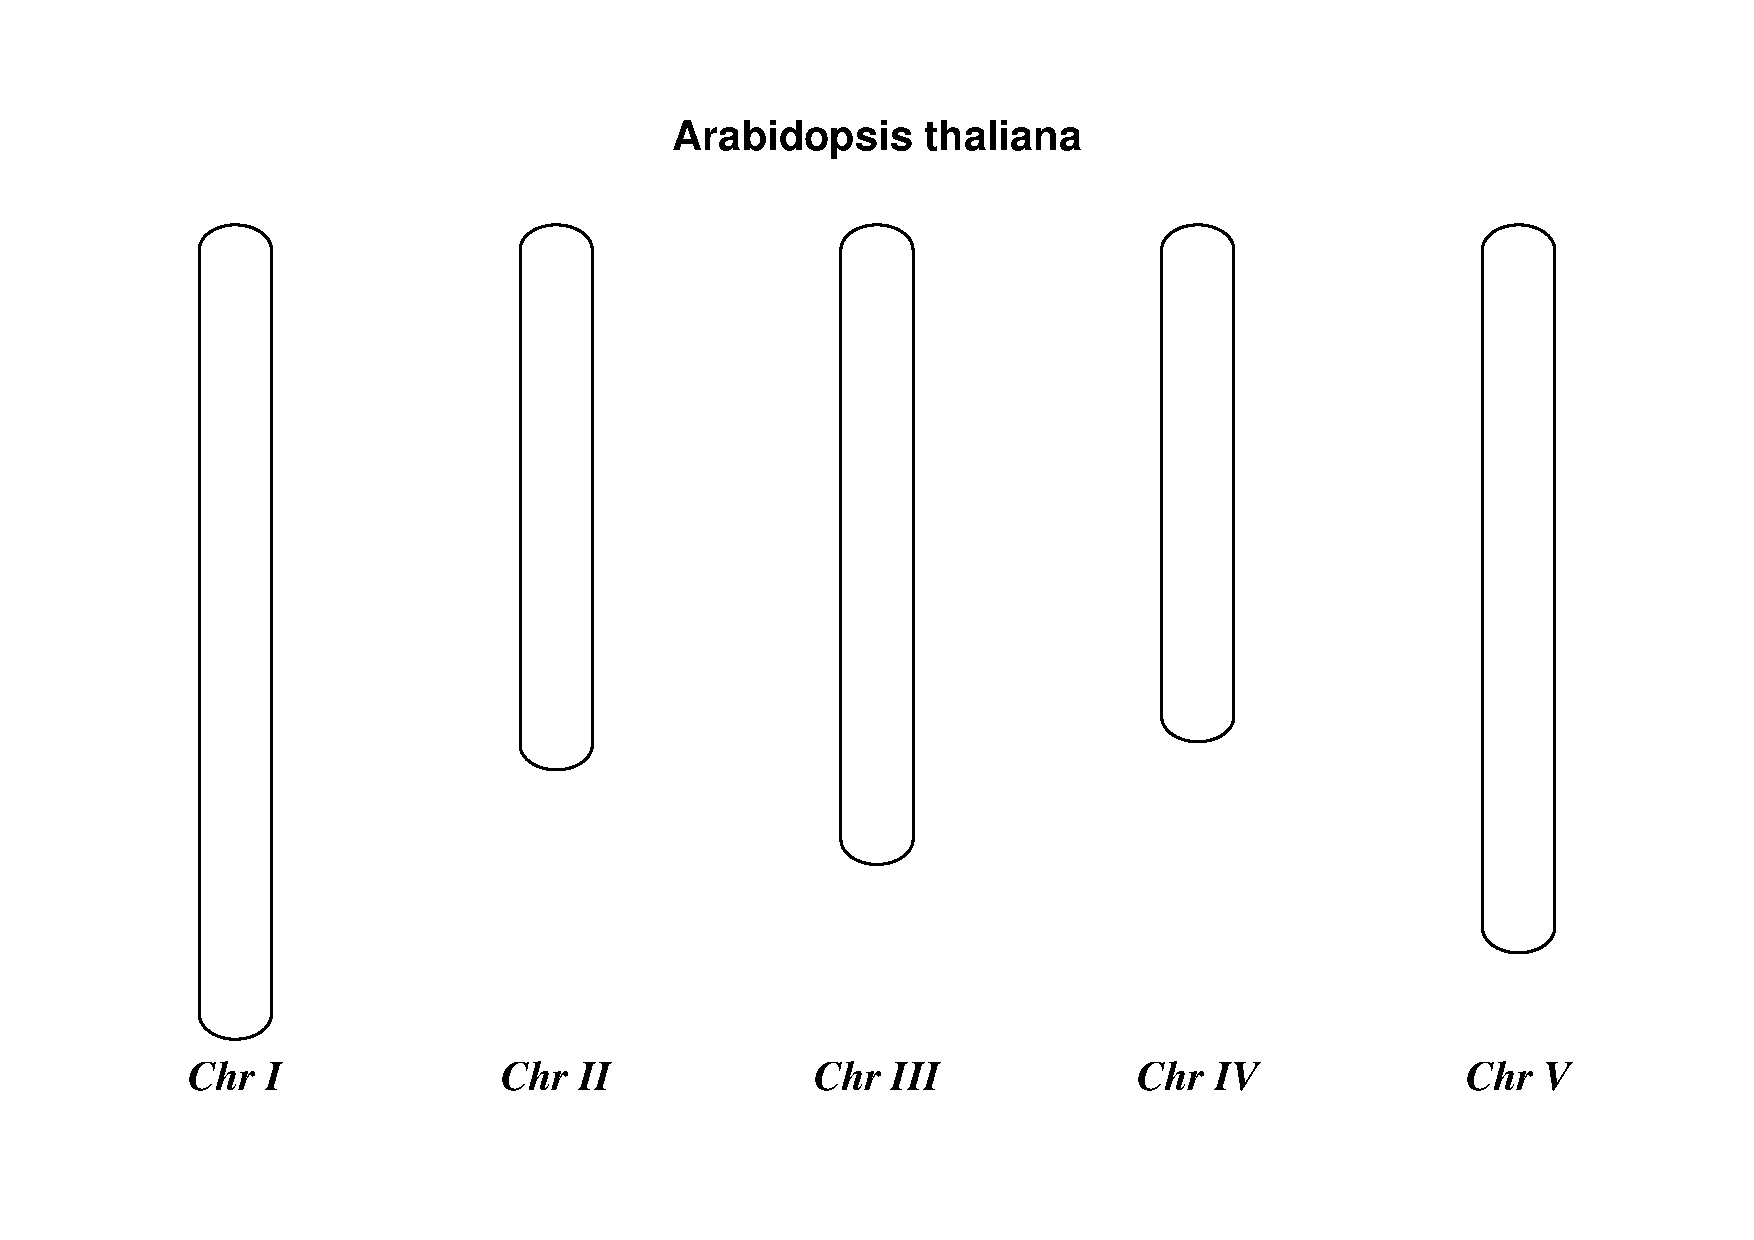
\includegraphics[scale=0.45]{images/simple_chrom.pdf}
\caption{Simple chromosome diagram for \textit{Arabidopsis thaliana}.}
\label{fig:simplechromosome}
\end{figure}
\begin{figure}[p]
\centering
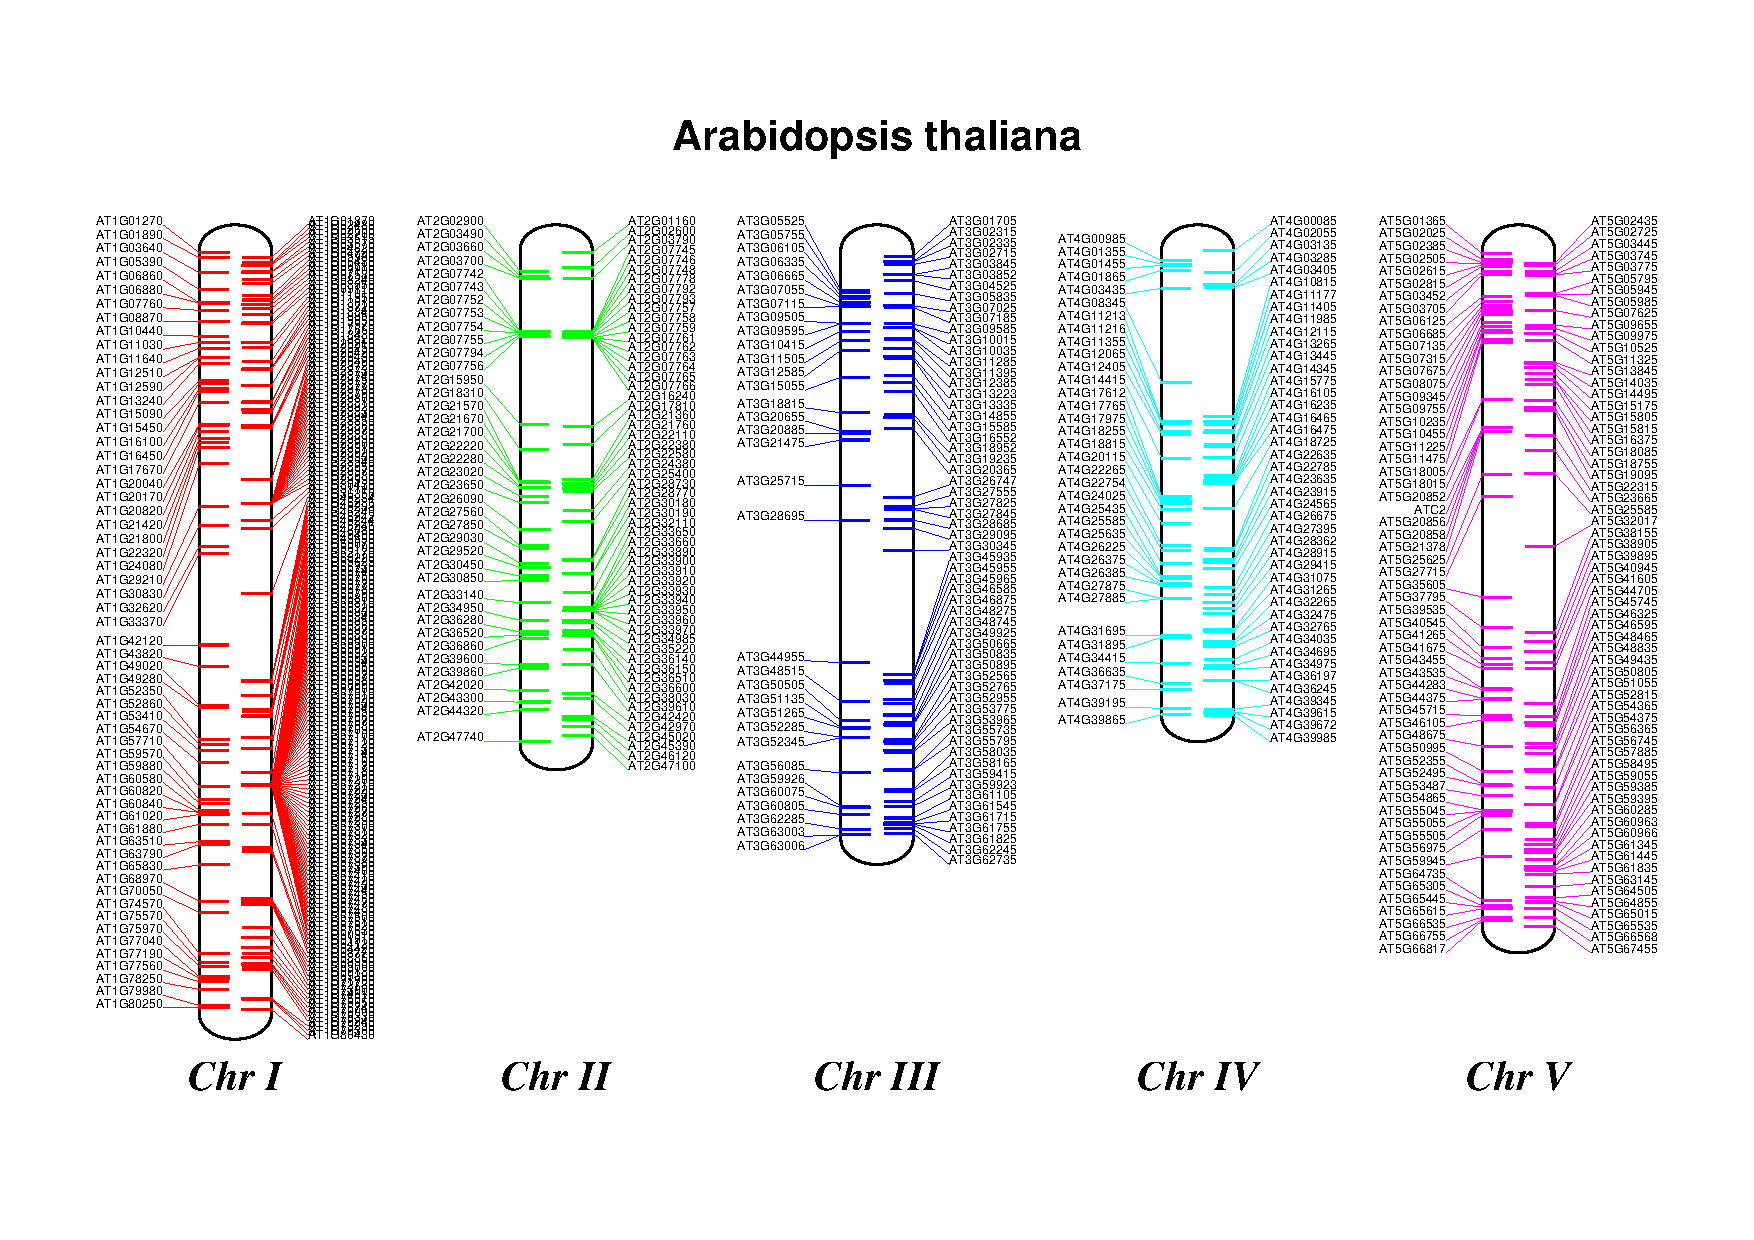
\includegraphics[scale=0.45]{images/tRNA_chrom.pdf}
\caption{Chromosome diagram for \textit{Arabidopsis thaliana} showing tRNA genes.}
\label{fig:trnachromosome}
\end{figure}
\end{latexonly}

You can skip this bit, but first I downloaded the five sequenced chromosomes
from the NCBI's FTP site
\url{ftp://ftp.ncbi.nlm.nih.gov/genomes/Arabidopsis_thaliana} and then parsed
them with \verb|Bio.SeqIO| to find out their lengths.  You could use the
GenBank files for this, but it is faster to use the FASTA files for the
whole chromosomes:

\begin{verbatim}
from Bio import SeqIO
entries = [("Chr I", "CHR_I/NC_003070.fna"),
           ("Chr II", "CHR_II/NC_003071.fna"),
           ("Chr III", "CHR_III/NC_003074.fna"),
           ("Chr IV", "CHR_IV/NC_003075.fna"),
           ("Chr V", "CHR_V/NC_003076.fna")]
for (name, filename) in entries:
   record = SeqIO.read(filename,"fasta")
   print name, len(record)
\end{verbatim}

\noindent This gave the lengths of the five chromosomes, which we'll now use in
the following short demonstration of the \verb|BasicChromosome| module:

\begin{verbatim}
from reportlab.lib.units import cm
from Bio.Graphics import BasicChromosome

entries = [("Chr I", 30432563),
           ("Chr II", 19705359),
           ("Chr III", 23470805),
           ("Chr IV", 18585042),
           ("Chr V", 26992728)]

max_len = 30432563 #Could compute this
telomere_length = 1000000 #For illustration
         
chr_diagram = BasicChromosome.Organism()
chr_diagram.page_size = (29.7*cm, 21*cm) #A4 landscape

for name, length in entries:
    cur_chromosome = BasicChromosome.Chromosome(name)
    #Set the scale to the MAXIMUM length plus the two telomeres in bp,
    #want the same scale used on all five chromosomes so they can be
    #compared to each other
    cur_chromosome.scale_num = max_len + 2 * telomere_length

    #Add an opening telomere
    start = BasicChromosome.TelomereSegment()
    start.scale = telomere_length
    cur_chromosome.add(start)

    #Add a body - using bp as the scale length here.
    body = BasicChromosome.ChromosomeSegment()
    body.scale = length
    cur_chromosome.add(body)

    #Add a closing telomere
    end = BasicChromosome.TelomereSegment(inverted=True)
    end.scale = telomere_length
    cur_chromosome.add(end)

    #This chromosome is done
    chr_diagram.add(cur_chromosome)

chr_diagram.draw("simple_chrom.pdf", "Arabidopsis thaliana")
\end{verbatim}

This should create a very simple PDF file, shown
\begin{htmlonly}
here:

%The blank lines above and below are important to trigger paragraph breaks
\imgsrc[width=650, height=460]{images/simple_chrom.png}

\end{htmlonly}
\begin{latexonly}
in Figure~\ref{fig:simplechromosome}.
\end{latexonly}
This example is deliberately short and sweet. The next example shows the
location of features of interest.

\subsection{Annotated Chromosomes}

Continuing from the previous example, let's also show the tRNA genes.
We'll get their locations by parsing the GenBank files for the five
\textit{Arabidopsis thaliana} chromosomes. You'll need to download these
files from the NCBI FTP site
\url{ftp://ftp.ncbi.nlm.nih.gov/genomes/Arabidopsis_thaliana},
and preserve the subdirectory names or edit the paths below:

\begin{verbatim}
from reportlab.lib.units import cm
from Bio import SeqIO
from Bio.Graphics import BasicChromosome

entries = [("Chr I", "CHR_I/NC_003070.gbk"),
           ("Chr II", "CHR_II/NC_003071.gbk"),
           ("Chr III", "CHR_III/NC_003074.gbk"),
           ("Chr IV", "CHR_IV/NC_003075.gbk"),
           ("Chr V", "CHR_V/NC_003076.gbk")]

max_len = 30432563 #Could compute this
telomere_length = 1000000 #For illustration

chr_diagram = BasicChromosome.Organism()
chr_diagram.page_size = (29.7*cm, 21*cm) #A4 landscape

for index, (name, filename) in enumerate(entries):
    record = SeqIO.read(filename,"genbank")
    length = len(record)
    features = [f for f in record.features if f.type=="tRNA"]
    #Record an Artemis style integer color in the feature's qualifiers,
    #1 = Black, 2 = Red, 3 = Green, 4 = blue, 5 =cyan, 6 = purple 
    for f in features: f.qualifiers["color"] = [index+2]

    cur_chromosome = BasicChromosome.Chromosome(name)
    #Set the scale to the MAXIMUM length plus the two telomeres in bp,
    #want the same scale used on all five chromosomes so they can be
    #compared to each other
    cur_chromosome.scale_num = max_len + 2 * telomere_length

    #Add an opening telomere
    start = BasicChromosome.TelomereSegment()
    start.scale = telomere_length
    cur_chromosome.add(start)

    #Add a body - again using bp as the scale length here.
    body = BasicChromosome.AnnotatedChromosomeSegment(length, features)
    body.scale = length
    cur_chromosome.add(body)

    #Add a closing telomere
    end = BasicChromosome.TelomereSegment(inverted=True)
    end.scale = telomere_length
    cur_chromosome.add(end)

    #This chromosome is done
    chr_diagram.add(cur_chromosome)

chr_diagram.draw("tRNA_chrom.pdf", "Arabidopsis thaliana")
\end{verbatim}

It might warn you about the labels being too close together - have a look
at the forward strand (right hand side) of Chr I, but it should create a
colorful PDF file, shown
\begin{htmlonly}
here:

%The blank lines above and below are important to trigger paragraph breaks
\imgsrc[width=650, height=460]{images/tRNA_chrom.png}

\end{htmlonly}
\begin{latexonly}
in Figure~\ref{fig:simplechromosome}.
\end{latexonly}

\chapter{Cookbook -- Cool things to do with it}
\label{chapter:cookbook}

Biopython now has two collections of ``cookbook'' examples -- this chapter
(which has been included in this tutorial for many years and has gradually
grown), and \url{http://biopython.org/wiki/Category:Cookbook} which is a
user contributed collection on our wiki.

We're trying to encourage Biopython users to contribute their own examples
to the wiki. In addition to helping the community, one direct benefit of
sharing an example like this is that you could also get some feedback on
the code from other Biopython users and developers - which could help you
improve all your Python code.

In the long term, we may end up moving all of the examples in this chapter
to the wiki, or elsewhere within the tutorial.

\section{Working with sequence files}
\label{seq:cookbook-sequences}

This section shows some more examples of sequence input/output, using the
\verb|Bio.SeqIO| module described in Chapter~\ref{chapter:Bio.SeqIO}.

\subsection{Filtering a sequence file}

Often you'll have a large file with many sequences in it (e.g. FASTA file
or genes, or a FASTQ or SFF file of reads), a separate shorter list of
the IDs for a subset of sequences of interest, and want to make a new
sequence file for this subset.

Let's say the list of IDs is in a simple text file, as the first word on
each line. This could be a tabular file where the first column is the ID.
Try something like this:

%not a doctest to avoid temp files being left behind, also no >>>
%makes it easier to copy and paste the example to a script file.
\begin{verbatim}
from Bio import SeqIO
input_file = "big_file.sff"
id_file = "short_list.txt"
output_file = "short_list.sff"
wanted = set(line.rstrip("\n").split(None,1)[0] for line in open(id_file))
print "Found %i unique identifiers in %s" % (len(wanted), id_file)
records = (r for r in SeqIO.parse(input_file, "sff") if r.id in wanted)
count = SeqIO.write(records, output_file, "sff")
print "Saved %i records from %s to %s" % (count, input_file, output_file)
if count < len(wanted):
    print "Warning %i IDs not found in %s" % (len(wanted)-count, input_file)
\end{verbatim}

Note that we use a Python \verb|set| rather than a \verb|list|, this makes
testing membership faster.

\subsection{Producing randomised genomes}

Let's suppose you are looking at genome sequence, hunting for some sequence
feature -- maybe extreme local GC\% bias, or possible restriction digest sites.
Once you've got your Python code working on the real genome it may be sensible
to try running the same search on randomised versions of the same genome for
statistical analysis (after all, any ``features'' you've found could just be
there just by chance).

For this discussion, we'll use the GenBank file for the pPCP1 plasmid from
\textit{Yersinia pestis biovar Microtus}.  The file is included with the
Biopython unit tests under the GenBank folder, or you can get it from our
website, \href{http://biopython.org/SRC/biopython/Tests/GenBank/NC_005816.gb}
{\texttt{NC\_005816.gb}}.  
This file contains one and only one record, so we can read it in as a
\verb|SeqRecord| using the \verb|Bio.SeqIO.read()| function:

%doctest ../Tests/GenBank
\begin{verbatim}
>>> from Bio import SeqIO
>>> original_rec = SeqIO.read("NC_005816.gb","genbank")
\end{verbatim}

So, how can we generate a shuffled versions of the original sequence?  I would
use the built in Python \verb|random| module for this, in particular the function
\verb|random.shuffle| -- but this works on a Python list.  Our sequence is a
\verb|Seq| object, so in order to shuffle it we need to turn it into a list:

%cont-doctest
\begin{verbatim}
>>> import random
>>> nuc_list = list(original_rec.seq)
>>> random.shuffle(nuc_list) #acts in situ!
\end{verbatim}

Now, in order to use \verb|Bio.SeqIO| to output the shuffled sequence, we need
to construct a new \verb|SeqRecord| with a new \verb|Seq| object using this
shuffled list.  In order to do this, we need to turn the list of nucleotides
(single letter strings) into a long string -- the standard Python way to do
this is with the string object's join method.

%cont-doctest
\begin{verbatim}
>>> from Bio.Seq import Seq
>>> from Bio.SeqRecord import SeqRecord
>>> shuffled_rec = SeqRecord(Seq("".join(nuc_list), original_rec.seq.alphabet),
...                          id="Shuffled", description="Based on %s" % original_rec.id)
\end{verbatim}

Let's put all these pieces together to make a complete Python script which
generates a single FASTA file containing 30 randomly shuffled versions of
the original sequence.

This first version just uses a big for loop and writes out the records one by one
(using the \verb|SeqRecord|'s format method described in
Section~\ref{sec:Bio.SeqIO-and-StringIO}):

\begin{verbatim}
import random
from Bio.Seq import Seq
from Bio.SeqRecord import SeqRecord
from Bio import SeqIO

original_rec = SeqIO.read("NC_005816.gb","genbank")

handle = open("shuffled.fasta", "w")
for i in range(30):
    nuc_list = list(original_rec.seq)
    random.shuffle(nuc_list)
    shuffled_rec = SeqRecord(Seq("".join(nuc_list), original_rec.seq.alphabet), \
                             id="Shuffled%i" % (i+1), \
                             description="Based on %s" % original_rec.id)
    handle.write(shuffled_rec.format("fasta"))
handle.close()
\end{verbatim}

Personally I prefer the following version using a function to shuffle the record
and a generator expression instead of the for loop:

\begin{verbatim}
import random
from Bio.Seq import Seq
from Bio.SeqRecord import SeqRecord
from Bio import SeqIO

def make_shuffle_record(record, new_id):
    nuc_list = list(record.seq)
    random.shuffle(nuc_list)
    return SeqRecord(Seq("".join(nuc_list), record.seq.alphabet), \
           id=new_id, description="Based on %s" % original_rec.id)
   
original_rec = SeqIO.read("NC_005816.gb","genbank")
shuffled_recs = (make_shuffle_record(original_rec, "Shuffled%i" % (i+1)) \
                 for i in range(30))
handle = open("shuffled.fasta", "w")
SeqIO.write(shuffled_recs, handle, "fasta")
handle.close()
\end{verbatim}

\subsection{Translating a FASTA file of CDS entries}
\label{sec:SeqIO-translate}
Suppose you've got an input file of CDS entries for some organism, and you
want to generate a new FASTA file containing their protein sequences.  i.e.
Take each nucleotide sequence from the original file, and translate it.
Back in Section~\ref{sec:translation} we saw how to use the \verb|Seq|
object's \verb|translate method|, and the optional \verb|cds| argument
which enables correct translation of alternative start codons.

We can combine this with \verb|Bio.SeqIO| as
shown in the reverse complement example in Section~\ref{sec:SeqIO-reverse-complement}.
The key point is that for each nucleotide \verb|SeqRecord|, we need to create
a protein \verb|SeqRecord| - and take care of naming it.

You can write you own function to do this, choosing suitable protein identifiers
for your sequences, and the appropriate genetic code.  In this example we just
use the default table and add a prefix to the identifier:

\begin{verbatim}
from Bio.SeqRecord import SeqRecord
def make_protein_record(nuc_record):
    """Returns a new SeqRecord with the translated sequence (default table)."""
    return SeqRecord(seq = nuc_record.seq.translate(cds=True), \
                     id = "trans_" + nuc_record.id, \
                     description = "translation of CDS, using default table")
\end{verbatim}

We can then use this function to turn the input nucleotide records into protein
records ready for output.  An elegant way and memory efficient way to do this
is with a generator expression:

\begin{verbatim}
from Bio import SeqIO
proteins = (make_protein_record(nuc_rec) for nuc_rec in \
            SeqIO.parse("coding_sequences.fasta", "fasta"))
SeqIO.write(proteins, "translations.fasta", "fasta")
\end{verbatim}

This should work on any FASTA file of complete coding sequences.
If you are working on partial coding sequences, you may prefer to use
\verb|nuc_record.seq.translate(to_stop=True)| in the example above, as
this wouldn't check for a valid start codon etc.

\subsection{Making the sequences in a FASTA file upper case}

Often you'll get data from collaborators as FASTA files, and sometimes the
sequences can be in a mixture of upper and lower case. In some cases this is
deliberate (e.g. lower case for poor quality regions), but usually it is not
important. You may want to edit the file to make everything consistent (e.g.
all upper case), and you can do this easily using the \verb|upper()| method
of the \verb|SeqRecord| object (added in Biopython 1.55):

\begin{verbatim}
from Bio import SeqIO
records = (rec.upper() for rec in SeqIO.parse("mixed.fas", "fasta"))
count = SeqIO.write(records, "upper.fas", "fasta")
print "Converted %i records to upper case" % count
\end{verbatim}

How does this work? The first line is just importing the \verb|Bio.SeqIO|
module. The second line is the interesting bit -- this is a Python
generator expression which gives an upper case version of each record
parsed from the input file (\texttt{mixed.fas}). In the third line we give
this generator expression to the \verb|Bio.SeqIO.write()| function and it
saves the new upper cases records to our output file (\texttt{upper.fas}).

The reason we use a generator expression (rather than a list or list
comprehension) is this means only one record is kept in memory at a time.
This can be really important if you are dealing with large files with
millions of entries.

\subsection{Sorting a sequence file}
\label{sec:SeqIO-sort}

Suppose you wanted to sort a sequence file by length (e.g. a set of
contigs from an assembly), and you are working with a file format like
FASTA or FASTQ which \verb|Bio.SeqIO| can read, write (and index).

If the file is small enough, you can load it all into memory at once
as a list of \verb|SeqRecord| objects, sort the list, and save it:

\begin{verbatim}
from Bio import SeqIO
records = list(SeqIO.parse("ls_orchid.fasta","fasta"))
records.sort(cmp=lambda x,y: cmp(len(x),len(y)))
SeqIO.write(records, "sorted_orchids.fasta", "fasta")
\end{verbatim}

The only clever bit is specifying a comparison function for how to
sort the records (here we sort them by length). If you wanted the
longest records first, you could flip the comparison or use the
reverse argument:

\begin{verbatim}
from Bio import SeqIO
records = list(SeqIO.parse("ls_orchid.fasta","fasta"))
records.sort(cmp=lambda x,y: cmp(len(y),len(x)))
SeqIO.write(records, "sorted_orchids.fasta", "fasta")
\end{verbatim}

Now that's pretty straight forward - but what happens if you have a
very large file and you can't load it all into memory like this?
For example, you might have some next-generation sequencing reads
to sort by length. This can be solved using the
\verb|Bio.SeqIO.index()| function.

\begin{verbatim}
from Bio import SeqIO
#Get the lengths and ids, and sort on length         
len_and_ids = sorted((len(rec), rec.id) for rec in \
                     SeqIO.parse("ls_orchid.fasta","fasta"))
ids = reversed([id for (length, id) in len_and_ids])
del len_and_ids	#free this memory
record_index = SeqIO.index("ls_orchid.fasta", "fasta")
records = (record_index[id] for id in ids)
SeqIO.write(records, "sorted.fasta", "fasta")
\end{verbatim}

First we scan through the file once using \verb|Bio.SeqIO.parse()|,
recording the record identifiers and their lengths in a list of tuples.
We then sort this list to get them in length order, and discard the lengths.
Using this sorted list of identifiers \verb|Bio.SeqIO.index()| allows us to
retrieve the records one by one, and we pass them to \verb|Bio.SeqIO.write()|
for output.

These examples all use \verb|Bio.SeqIO| to parse the records into
\verb|SeqRecord| objects which are output using \verb|Bio.SeqIO.write()|.
What if you want to sort a file format which \verb|Bio.SeqIO.write()| doesn't
support, like the plain text SwissProt format? Here is an alternative
solution using the \verb|get_raw()| method added to \verb|Bio.SeqIO.index()|
in Biopython 1.54 (see Section~\ref{sec:seqio-index-getraw}).

\begin{verbatim}
from Bio import SeqIO
#Get the lengths and ids, and sort on length         
len_and_ids = sorted((len(rec), rec.id) for rec in \
                     SeqIO.parse("ls_orchid.fasta","fasta"))
ids = reversed([id for (length, id) in len_and_ids])
del len_and_ids	#free this memory
record_index = SeqIO.index("ls_orchid.fasta", "fasta")
handle = open("sorted.fasta", "w")
for id in ids:
    handle.write(record_index.get_raw(id))
handle.close()
\end{verbatim}

As a bonus, because doesn't parse the data into \verb|SeqRecord| objects
a second time it should be faster.

\subsection{Simple quality filtering for FASTQ files}
\label{sec:FASTQ-filtering-example}

The FASTQ file format was introduced at Sanger and is now widely used for
holding nucleotide sequencing reads together with their quality scores.
FASTQ files (and the related QUAL files) are an excellent example of
per-letter-annotation, because for each nucleotide in the sequence there is
an associated quality score.  Any per-letter-annotation is held in a
\verb|SeqRecord| in the \verb|letter_annotations| dictionary as a list,
tuple or string (with the same number of elements as the sequence length).

One common task is taking a large set of sequencing reads and filtering them
(or cropping them) based on their quality scores.
The following example is very simplistic, but should illustrate the basics of
working with quality data in a \verb|SeqRecord| object.  All we are going to
do here is read in a file of FASTQ data, and filter it to pick out only those
records whose PHRED quality scores are all above some threshold (here 20).

For this example we'll use some real data downloaded from the ENA sequence
read archive,
\url{ftp://ftp.sra.ebi.ac.uk/vol1/fastq/SRR020/SRR020192/SRR020192.fastq.gz}
(2MB) which unzips to a 19MB file \texttt{SRR020192.fastq}. This is some
Roche 454 GS FLX single end data from virus infected California sea lions
(see \url{http://www.ebi.ac.uk/ena/data/view/SRS004476} for details).

First, let's count the reads:

\begin{verbatim}
from Bio import SeqIO
count = 0
for rec in SeqIO.parse("SRR020192.fastq", "fastq"):
    count += 1
print "%i reads" % count
\end{verbatim}

\noindent Now let's do a simple filtering for a minimum PHRED quality of 20:

\begin{verbatim}
from Bio import SeqIO
good_reads = (rec for rec in \
              SeqIO.parse("SRR020192.fastq", "fastq") \
              if min(rec.letter_annotations["phred_quality"]) >= 20)
count = SeqIO.write(good_reads, "good_quality.fastq", "fastq")
print "Saved %i reads" % count
\end{verbatim}

\noindent This pulled out only $14580$ reads out of the $41892$ present.
A more sensible thing to do would be to quality trim the reads, but this
is intended as an example only.

FASTQ files can contain millions of entries, so it is best to avoid loading
them all into memory at once.  This example uses a generator expression, which
means only one \verb|SeqRecord| is created at a time - avoiding any memory
limitations.

\subsection{Trimming off primer sequences}
\label{sec:FASTQ-slicing-off-primer}

For this example we're going to pretend that \texttt{GATGACGGTGT} is a 5' primer
sequence we want to look for in some FASTQ formatted read data.  As in the example
above, we'll use the \texttt{SRR020192.fastq} file downloaded from the ENA
(\url{ftp://ftp.sra.ebi.ac.uk/vol1/fastq/SRR020/SRR020192/SRR020192.fastq.gz}).
The same approach would work with any other supported file format (e.g. FASTA files).

This code uses \verb|Bio.SeqIO| with a generator expression (to avoid loading
all the sequences into memory at once), and the \verb|Seq| object's
\verb|startswith| method to see if the read starts with the primer sequence:

\begin{verbatim}
from Bio import SeqIO
primer_reads = (rec for rec in \
                SeqIO.parse("SRR020192.fastq", "fastq") \
                if rec.seq.startswith("GATGACGGTGT"))
count = SeqIO.write(primer_reads, "with_primer.fastq", "fastq")
print "Saved %i reads" % count
\end{verbatim}

\noindent That should find $13819$ reads from \texttt{SRR014849.fastq} and save them to
a new FASTQ file, \texttt{with\_primer.fastq}.

Now suppose that instead you wanted to make a FASTQ file containing these reads
but with the primer sequence removed?  That's just a small change as we can slice the
\verb|SeqRecord| (see Section~\ref{sec:SeqRecord-slicing}) to remove the first eleven
letters (the length of our primer):

\begin{verbatim}
from Bio import SeqIO
trimmed_primer_reads = (rec[11:] for rec in \
                        SeqIO.parse("SRR020192.fastq", "fastq") \
                        if rec.seq.startswith("GATGACGGTGT"))
count = SeqIO.write(trimmed_primer_reads, "with_primer_trimmed.fastq", "fastq")
print "Saved %i reads" % count
\end{verbatim}

\noindent Again, that should pull out the $13819$ reads from \texttt{SRR020192.fastq},
but this time strip off the first ten characters, and save them to another new
FASTQ file, \texttt{with\_primer\_trimmed.fastq}.

Finally, suppose you want to create a new FASTQ file where these reads have
their primer removed, but all the other reads are kept as they were?
If we want to still use a generator expression, it is probably clearest to
define our own trim function:

\begin{verbatim}
from Bio import SeqIO
def trim_primer(record, primer):
    if record.seq.startswith(primer):
        return record[len(primer):]
    else:
        return record

trimmed_reads = (trim_primer(record, "GATGACGGTGT") for record in \
                 SeqIO.parse("SRR020192.fastq", "fastq"))
count = SeqIO.write(trimmed_reads, "trimmed.fastq", "fastq")
print "Saved %i reads" % count
\end{verbatim}

This takes longer, as this time the output file contains all $41892$ reads.
Again, we're used a generator expression to avoid any memory problems.
You could alternatively use a generator function rather than a generator
expression.

\begin{verbatim}
from Bio import SeqIO
def trim_primers(records, primer):
    """Removes perfect primer sequences at start of reads.
    
    This is a generator function, the records argument should
    be a list or iterator returning SeqRecord objects.
    """
    len_primer = len(primer) #cache this for later
    for record in records:
        if record.seq.startswith(primer):
            yield record[len_primer:]
        else:
            yield record

original_reads = SeqIO.parse("SRR020192.fastq", "fastq")
trimmed_reads = trim_primers(original_reads, "GATGACGGTGT")
count = SeqIO.write(trimmed_reads, "trimmed.fastq", "fastq") 
print "Saved %i reads" % count
\end{verbatim}

This form is more flexible if you want to do something more complicated
where only some of the records are retained -- as shown in the next example.

\subsection{Trimming off adaptor sequences}
\label{sec:FASTQ-slicing-off-adaptor}

This is essentially a simple extension to the previous example. We are going
to going to pretend \texttt{GATGACGGTGT} is an adaptor sequence in some FASTQ
formatted read data, again the \texttt{SRR020192.fastq} file from the NCBI
(\url{ftp://ftp.sra.ebi.ac.uk/vol1/fastq/SRR020/SRR020192/SRR020192.fastq.gz}).

This time however, we will look for the sequence \emph{anywhere} in the reads,
not just at the very beginning:

\begin{verbatim}
from Bio import SeqIO

def trim_adaptors(records, adaptor):
    """Trims perfect adaptor sequences.
    
    This is a generator function, the records argument should
    be a list or iterator returning SeqRecord objects.
    """
    len_adaptor = len(adaptor) #cache this for later
    for record in records:
        index = record.seq.find(adaptor)
        if index == -1:
            #adaptor not found, so won't trim
            yield record
        else:
            #trim off the adaptor
            yield record[index+len_adaptor:]

original_reads = SeqIO.parse("SRR020192.fastq", "fastq")
trimmed_reads = trim_adaptors(original_reads, "GATGACGGTGT")
count = SeqIO.write(trimmed_reads, "trimmed.fastq", "fastq") 
print "Saved %i reads" % count
\end{verbatim}

Because we are using a FASTQ input file in this example, the \verb|SeqRecord|
objects have per-letter-annotation for the quality scores. By slicing the
\verb|SeqRecord| object the appropriate scores are used on the trimmed
records, so we can output them as a FASTQ file too.

Compared to the output of the previous example where we only looked for
a primer/adaptor at the start of each read, you may find some of the
trimmed reads are quite short after trimming (e.g. if the adaptor was
found in the middle rather than near the start). So, let's add a minimum
length requirement as well:

\begin{verbatim}
from Bio import SeqIO

def trim_adaptors(records, adaptor, min_len):
    """Trims perfect adaptor sequences, checks read length.
    
    This is a generator function, the records argument should
    be a list or iterator returning SeqRecord objects.
    """
    len_adaptor = len(adaptor) #cache this for later
    for record in records:
        len_record = len(record) #cache this for later
        if len(record) < min_len:
           #Too short to keep
           continue
        index = record.seq.find(adaptor)
        if index == -1:
            #adaptor not found, so won't trim
            yield record
        elif len_record - index - len_adaptor >= min_len:
            #after trimming this will still be long enough
            yield record[index+len_adaptor:]

original_reads = SeqIO.parse("SRR020192.fastq", "fastq")
trimmed_reads = trim_adaptors(original_reads, "GATGACGGTGT", 100)
count = SeqIO.write(trimmed_reads, "trimmed.fastq", "fastq") 
print "Saved %i reads" % count
\end{verbatim}

By changing the format names, you could apply this to FASTA files instead.
This code also could be extended to do a fuzzy match instead of an exact
match (maybe using a pairwise alignment, or taking into account the read
quality scores), but that will be much slower.

\subsection{Converting FASTQ files}
\label{sec:SeqIO-fastq-conversion}

Back in Section~\ref{sec:SeqIO-conversion} we showed how to use
\verb|Bio.SeqIO| to convert between two file formats. Here we'll go into a
little more detail regarding FASTQ files which are used in second generation
DNA sequencing. Please refer to Cock \textit{et al.} (2009) \cite{cock2009nar}
for a longer description. FASTQ files store both the DNA sequence (as a string)
and the associated read qualities. 

PHRED scores (used in most FASTQ files, and also in QUAL files, ACE files
and SFF files) have become a \textit{de facto} standard for representing
the probability of a sequencing error (here denoted by $P_e$) at a given
base using a simple base ten log transformation:

\begin{equation}
Q_{\textrm{PHRED}} = - 10 \times \textrm{log}_{10} ( P_e )
\end{equation}

This means a wrong read ($P_e = 1$) gets a PHRED quality of $0$, while a very
good read like $P_e = 0.00001$ gets a PHRED quality of $50$. While for raw
sequencing data qualities higher than this are rare, with post processing
such as read mapping or assembly, qualities of up to about $90$ are possible
(indeed, the MAQ tool allows for PHRED scores in the range 0 to 93 inclusive).

The FASTQ format has the potential to become a \textit{de facto} standard for
storing the letters and quality scores for a sequencing read in a single plain
text file. The only fly in the ointment is that there are at least three
versions of the FASTQ format which are incompatible and difficult to
distinguish...

\begin{enumerate}
\item The original Sanger FASTQ format uses PHRED qualities encoded with an
ASCII offset of 33. The NCBI are using this format in their Short Read
Archive. We call this the \texttt{fastq} (or \texttt{fastq-sanger}) format
in \verb|Bio.SeqIO|.
\item Solexa (later bought by Illumina) introduced their own version using
Solexa qualities encoded with an ASCII offset of 64. We call this the
\texttt{fastq-solexa} format.
\item Illumina pipeline 1.3 onwards produces FASTQ files with PHRED qualities
(which is more consistent), but encoded with an ASCII offset of 64. We call
this the \texttt{fastq-illumina} format.
\end{enumerate}

The Solexa quality scores are defined using a different log transformation:

\begin{equation}
Q_{\textrm{Solexa}} = - 10 \times \textrm{log}_{10} \left( \frac{P_e}{1-P_e} \right)
\end{equation}

Given Solexa/Illumina have now moved to using PHRED scores in version 1.3 of
their pipeline, the Solexa quality scores will gradually fall out of use.
If you equate the error estimates ($P_e$) these two equations allow conversion
between the two scoring systems - and Biopython includes functions to do this
in the \verb|Bio.SeqIO.QualityIO| module, which are called if you use
\verb|Bio.SeqIO| to convert an old Solexa/Illumina file into a standard Sanger
FASTQ file:

\begin{verbatim}
from Bio import SeqIO
SeqIO.convert("solexa.fastq", "fastq-solexa", "standard.fastq", "fastq")
\end{verbatim}

If you want to convert a new Illumina 1.3+ FASTQ file, all that gets changed
is the ASCII offset because although encoded differently the scores are all
PHRED qualities:

\begin{verbatim}
from Bio import SeqIO
SeqIO.convert("illumina.fastq", "fastq-illumina", "standard.fastq", "fastq")
\end{verbatim}

Note that using \verb|Bio.SeqIO.convert()| like this is \emph{much} faster
than combining \verb|Bio.SeqIO.parse()| and \verb|Bio.SeqIO.write()|
because optimised code is used for converting between FASTQ variants
(and also for FASTQ to FASTA conversion).

For good quality reads, PHRED and Solexa scores are approximately equal,
which means since both the \texttt{fasta-solexa} and \texttt{fastq-illumina}
formats use an ASCII offset of 64 the files are almost the same. This was a
deliberate design choice by Illumina, meaning applications expecting the old
\texttt{fasta-solexa} style files will probably be OK using the newer
\texttt{fastq-illumina} files (on good data). Of course, both variants are
very different from the original FASTQ standard as used by Sanger,
the NCBI, and elsewhere (format name \texttt{fastq} or \texttt{fastq-sanger}).

For more details, see the built in help (also \href{http://www.biopython.org/DIST/docs/api/Bio.SeqIO.QualityIO-module.html}{online}):

\begin{verbatim}
>>> from Bio.SeqIO import QualityIO
>>> help(QualityIO)
...
\end{verbatim}

\subsection{Converting FASTA and QUAL files into FASTQ files}
\label{sec:SeqIO-fasta-qual-conversion}

FASTQ files hold \emph{both} sequences and their quality strings.
FASTA files hold \emph{just} sequences, while QUAL files hold \emph{just}
the qualities. Therefore a single FASTQ file can be converted to or from
\emph{paired} FASTA and QUAL files.

Going from FASTQ to FASTA is easy:

\begin{verbatim}
from Bio import SeqIO
SeqIO.convert("example.fastq", "fastq", "example.fasta", "fasta")
\end{verbatim}

Going from FASTQ to QUAL is also easy:

\begin{verbatim}
from Bio import SeqIO
SeqIO.convert("example.fastq", "fastq", "example.qual", "qual")
\end{verbatim}

However, the reverse is a little more tricky. You can use \verb|Bio.SeqIO.parse()|
to iterate over the records in a \emph{single} file, but in this case we have
two input files. There are several strategies possible, but assuming that the
two files are really paired the most memory efficient way is to loop over both
together. The code is a little fiddly, so we provide a function called
\verb|PairedFastaQualIterator| in the \verb|Bio.SeqIO.QualityIO| module to do
this. This takes two handles (the FASTA file and the QUAL file) and returns
a \verb|SeqRecord| iterator:

\begin{verbatim}
from Bio.SeqIO.QualityIO import PairedFastaQualIterator
for record in PairedFastaQualIterator(open("example.fasta"), open("example.qual")):
   print record
\end{verbatim}

This function will check that the FASTA and QUAL files are consistent (e.g.
the records are in the same order, and have the same sequence length).
You can combine this with the \verb|Bio.SeqIO.write()| function to convert a
pair of FASTA and QUAL files into a single FASTQ files:

\begin{verbatim}
from Bio import SeqIO
from Bio.SeqIO.QualityIO import PairedFastaQualIterator
handle = open("temp.fastq", "w") #w=write
records = PairedFastaQualIterator(open("example.fasta"), open("example.qual"))
count = SeqIO.write(records, handle, "fastq")
handle.close()
print "Converted %i records" % count
\end{verbatim}

\subsection{Indexing a FASTQ file}
\label{sec:fastq-indexing}

FASTQ files are often very large, with millions of reads in them. Due to the
sheer amount of data, you can't load all the records into memory at once.
This is why the examples above (filtering and trimming) iterate over the file
looking at just one \verb|SeqRecord| at a time.

However, sometimes you can't use a big loop or an iterator - you may need
random access to the reads. Here the \verb|Bio.SeqIO.index()| function
may prove very helpful, as it allows you to access any read in the FASTQ file
by its name (see Section~\ref{sec:SeqIO-index}).

Again we'll use the \texttt{SRR020192.fastq} file from the ENA
(\url{ftp://ftp.sra.ebi.ac.uk/vol1/fastq/SRR020/SRR020192/SRR020192.fastq.gz}),
although this is actually quite a small FASTQ file with less than $50,000$ reads:

\begin{verbatim}
>>> from Bio import SeqIO
>>> fq_dict = SeqIO.index("SRR020192.fastq", "fastq")
>>> len(fq_dict)
41892
>>> fq_dict.keys()[:4]
['SRR020192.38240', 'SRR020192.23181', 'SRR020192.40568', 'SRR020192.23186']
>>> fq_dict["SRR020192.23186"].seq
Seq('GTCCCAGTATTCGGATTTGTCTGCCAAAACAATGAAATTGACACAGTTTACAAC...CCG', SingleLetterAlphabet())
\end{verbatim}

When testing this on a FASTQ file with seven million reads,
indexing took about a minute, but record access was almost instant.

The example in Section~\ref{sec:SeqIO-sort} show how you can use the
\verb|Bio.SeqIO.index()| function to sort a large FASTA file -- this
could also be used on FASTQ files.

\subsection{Converting SFF files}
\label{sec:SeqIO-sff-conversion}

If you work with 454 (Roche) sequence data, you will probably have access
to the raw data as a Standard Flowgram Format (SFF) file. This contains
the sequence reads (called bases) with quality scores and the original
flow information.

A common task is to convert from SFF to a pair of FASTA and QUAL files,
or to a single FASTQ file. These operations are trivial using the
\verb|Bio.SeqIO.convert()| function (see Section~\ref{sec:SeqIO-conversion}):

\begin{verbatim}
>>> from Bio import SeqIO
>>> SeqIO.convert("E3MFGYR02_random_10_reads.sff", "sff", "reads.fasta", "fasta")
10
>>> SeqIO.convert("E3MFGYR02_random_10_reads.sff", "sff", "reads.qual", "qual")
10
>>> SeqIO.convert("E3MFGYR02_random_10_reads.sff", "sff", "reads.fastq", "fastq")
10
\end{verbatim}

\noindent Remember the convert function returns the number of records, in
this example just ten. This will give you the \emph{untrimmed} reads, where
the leading and trailing poor quality sequence or adaptor will be in lower
case. If you want the \emph{trimmed} reads (using the clipping information
recorded within the SFF file) use this:

\begin{verbatim}
>>> from Bio import SeqIO
>>> SeqIO.convert("E3MFGYR02_random_10_reads.sff", "sff-trim", "trimmed.fasta", "fasta")
10
>>> SeqIO.convert("E3MFGYR02_random_10_reads.sff", "sff-trim", "trimmed.qual", "qual")
10
>>> SeqIO.convert("E3MFGYR02_random_10_reads.sff", "sff-trim", "trimmed.fastq", "fastq")
10
\end{verbatim}

If you run Linux, you could ask Roche for a copy of their ``off instrument''
tools (often referred to as the Newbler tools). This offers an alternative way to
do SFF to FASTA or QUAL conversion at the command line (but currently FASTQ output
is not supported), e.g.

\begin{verbatim}
$ sffinfo -seq -notrim E3MFGYR02_random_10_reads.sff > reads.fasta
$ sffinfo -qual -notrim E3MFGYR02_random_10_reads.sff > reads.qual
$ sffinfo -seq -trim E3MFGYR02_random_10_reads.sff > trimmed.fasta
$ sffinfo -qual -trim E3MFGYR02_random_10_reads.sff > trimmed.qual
\end{verbatim}

\noindent The way Biopython uses mixed case sequence strings to represent
the trimming points deliberately mimics what the Roche tools do.

For more information on the Biopython SFF support, consult the built in help:

\begin{verbatim}
>>> from Bio.SeqIO import SffIO
>>> help(SffIO)
...
\end{verbatim}

\subsection{Identifying open reading frames}

A very simplistic first step at identifying possible genes is to look for
open reading frames (ORFs).  By this we mean look in all six frames for long
regions without stop codons -- an ORF is just a region of nucleotides with
no in frame stop codons.

Of course, to find a gene you would also need to worry about locating a start
codon, possible promoters -- and in Eukaryotes there are introns to worry about
too.  However, this approach is still useful in viruses and Prokaryotes.

To show how you might approach this with Biopython, we'll need a sequence to
search, and as an example we'll again use the bacterial plasmid -- although
this time we'll start with a plain FASTA file with no pre-marked genes:
\href{http://biopython.org/SRC/biopython/Tests/GenBank/NC_005816.fna}
{\texttt{NC\_005816.fna}}. This is a bacterial sequence, so we'll want to use
NCBI codon table 11 (see Section~\ref{sec:translation} about translation).

%doctest ../Tests/GenBank
\begin{verbatim}
>>> from Bio import SeqIO 
>>> record = SeqIO.read("NC_005816.fna","fasta")
>>> table = 11
>>> min_pro_len = 100
\end{verbatim}

Here is a neat trick using the \verb|Seq| object's \verb|split| method to
get a list of all the possible ORF translations in the six reading frames:

%cont-doctest
\begin{verbatim}
>>> for strand, nuc in [(+1, record.seq), (-1, record.seq.reverse_complement())]:
...     for frame in range(3):
...         for pro in nuc[frame:].translate(table).split("*"):
...             if len(pro) >= min_pro_len:
...                 print "%s...%s - length %i, strand %i, frame %i" \
...                       % (pro[:30], pro[-3:], len(pro), strand, frame)
GCLMKKSSIVATIITILSGSANAASSQLIP...YRF - length 315, strand 1, frame 0
KSGELRQTPPASSTLHLRLILQRSGVMMEL...NPE - length 285, strand 1, frame 1
GLNCSFFSICNWKFIDYINRLFQIIYLCKN...YYH - length 176, strand 1, frame 1
VKKILYIKALFLCTVIKLRRFIFSVNNMKF...DLP - length 165, strand 1, frame 1
NQIQGVICSPDSGEFMVTFETVMEIKILHK...GVA - length 355, strand 1, frame 2
RRKEHVSKKRRPQKRPRRRRFFHRLRPPDE...PTR - length 128, strand 1, frame 2
TGKQNSCQMSAIWQLRQNTATKTRQNRARI...AIK - length 100, strand 1, frame 2
QGSGYAFPHASILSGIAMSHFYFLVLHAVK...CSD - length 114, strand -1, frame 0
IYSTSEHTGEQVMRTLDEVIASRSPESQTR...FHV - length 111, strand -1, frame 0
WGKLQVIGLSMWMVLFSQRFDDWLNEQEDA...ESK - length 125, strand -1, frame 1
RGIFMSDTMVVNGSGGVPAFLFSGSTLSSY...LLK - length 361, strand -1, frame 1
WDVKTVTGVLHHPFHLTFSLCPEGATQSGR...VKR - length 111, strand -1, frame 1
LSHTVTDFTDQMAQVGLCQCVNVFLDEVTG...KAA - length 107, strand -1, frame 2
RALTGLSAPGIRSQTSCDRLRELRYVPVSL...PLQ - length 119, strand -1, frame 2
\end{verbatim}

Note that here we are counting the frames from the 5' end (start) of
\emph{each} strand. It is sometimes easier to always count from the 5' end
(start) of the \emph{forward} strand.

You could easily edit the above loop based code to build up a list of the
candidate proteins, or convert this to a list comprehension.  Now, one thing
this code doesn't do is keep track of where the proteins are.

You could tackle this in several ways.  For example, the following code tracks
the locations in terms of the protein counting, and converts back to the
parent sequence by multiplying by three, then adjusting for the frame and
strand:

\begin{verbatim}
from Bio import SeqIO 
record = SeqIO.read("NC_005816.gb","genbank")
table = 11
min_pro_len = 100

def find_orfs_with_trans(seq, trans_table, min_protein_length):
    answer = []
    seq_len = len(seq)
    for strand, nuc in [(+1, seq), (-1, seq.reverse_complement())]:
        for frame in range(3):
            trans = str(nuc[frame:].translate(trans_table))
            trans_len = len(trans)
            aa_start = 0
            aa_end = 0
            while aa_start < trans_len:
                aa_end = trans.find("*", aa_start)
                if aa_end == -1:
                    aa_end = trans_len
                if aa_end-aa_start >= min_protein_length:
                    if strand == 1:
                        start = frame+aa_start*3
                        end = min(seq_len,frame+aa_end*3+3)
                    else:
                        start = seq_len-frame-aa_end*3-3
                        end = seq_len-frame-aa_start*3                        
                    answer.append((start, end, strand,
                                   trans[aa_start:aa_end]))
                aa_start = aa_end+1
    answer.sort()
    return answer

orf_list = find_orfs_with_trans(record.seq, table, min_pro_len)
for start, end, strand, pro in orf_list:
    print "%s...%s - length %i, strand %i, %i:%i" \
          % (pro[:30], pro[-3:], len(pro), strand, start, end)
\end{verbatim}

\noindent And the output:

\begin{verbatim}
NQIQGVICSPDSGEFMVTFETVMEIKILHK...GVA - length 355, strand 1, 41:1109
WDVKTVTGVLHHPFHLTFSLCPEGATQSGR...VKR - length 111, strand -1, 491:827
KSGELRQTPPASSTLHLRLILQRSGVMMEL...NPE - length 285, strand 1, 1030:1888
RALTGLSAPGIRSQTSCDRLRELRYVPVSL...PLQ - length 119, strand -1, 2830:3190
RRKEHVSKKRRPQKRPRRRRFFHRLRPPDE...PTR - length 128, strand 1, 3470:3857
GLNCSFFSICNWKFIDYINRLFQIIYLCKN...YYH - length 176, strand 1, 4249:4780
RGIFMSDTMVVNGSGGVPAFLFSGSTLSSY...LLK - length 361, strand -1, 4814:5900
VKKILYIKALFLCTVIKLRRFIFSVNNMKF...DLP - length 165, strand 1, 5923:6421
LSHTVTDFTDQMAQVGLCQCVNVFLDEVTG...KAA - length 107, strand -1, 5974:6298
GCLMKKSSIVATIITILSGSANAASSQLIP...YRF - length 315, strand 1, 6654:7602
IYSTSEHTGEQVMRTLDEVIASRSPESQTR...FHV - length 111, strand -1, 7788:8124
WGKLQVIGLSMWMVLFSQRFDDWLNEQEDA...ESK - length 125, strand -1, 8087:8465
TGKQNSCQMSAIWQLRQNTATKTRQNRARI...AIK - length 100, strand 1, 8741:9044
QGSGYAFPHASILSGIAMSHFYFLVLHAVK...CSD - length 114, strand -1, 9264:9609
\end{verbatim}

If you comment out the sort statement, then the protein sequences will be
shown in the same order as before, so you can check this is doing the same
thing.  Here we have sorted them by location to make it easier to compare
to the actual annotation in the GenBank file (as visualised in
Section~\ref{sec:gd_nice_example}).

If however all you want to find are the locations of the open reading frames,
then it is a waste of time to translate every possible codon, including doing
the reverse complement to search the reverse strand too.  All you need to do
is search for the possible stop codons (and their reverse complements).  Using
regular expressions is an obvious approach here (see the Python module
\verb|re|). These are an extremely powerful (but rather complex) way of
describing search strings, which are supported in lots of programming
languages and also command line tools like \texttt{grep} as well). You can
find whole books about this topic!


\section{Sequence parsing plus simple plots}
\label{seq:sequence-parsing-plus-pylab}

This section shows some more examples of sequence parsing, using the \verb|Bio.SeqIO|
module described in Chapter~\ref{chapter:Bio.SeqIO}, plus the Python library matplotlib's \verb|pylab| plotting interface (see \href{http://matplotlib.sourceforge.net/}{the matplotlib website for a tutorial}).  Note that to follow these examples you will need matplotlib installed - but without it you can still try the data parsing bits.

\subsection{Histogram of sequence lengths}

There are lots of times when you might want to visualise the distribution of sequence
lengths in a dataset -- for example the range of contig sizes in a genome assembly
project.  In this example we'll reuse our orchid FASTA file \href{http://biopython.org/DIST/docs/tutorial/examples/ls_orchid.fasta}{\tt ls\_orchid.fasta} which has only 94 sequences.

First of all, we will use \verb|Bio.SeqIO| to parse the FASTA file and compile a list
of all the sequence lengths.  You could do this with a for loop, but I find a list
comprehension more pleasing:

\begin{verbatim}
>>> from Bio import SeqIO
>>> sizes = [len(rec) for rec in SeqIO.parse("ls_orchid.fasta", "fasta")]
>>> len(sizes), min(sizes), max(sizes)
(94, 572, 789)
>>> sizes
[740, 753, 748, 744, 733, 718, 730, 704, 740, 709, 700, 726, ..., 592]
\end{verbatim}

Now that we have the lengths of all the genes (as a list of integers), we can use the
matplotlib histogram function to display it.

\begin{verbatim}
from Bio import SeqIO
sizes = [len(rec) for rec in SeqIO.parse("ls_orchid.fasta", "fasta")]

import pylab
pylab.hist(sizes, bins=20)
pylab.title("%i orchid sequences\nLengths %i to %i" \
            % (len(sizes),min(sizes),max(sizes)))
pylab.xlabel("Sequence length (bp)")
pylab.ylabel("Count")
pylab.show()
\end{verbatim}

%
% Have a HTML version and a PDF version to display nicely...
%
\begin{htmlonly}
\noindent That should pop up a new window containing the following graph:

\imgsrc[width=600, height=450]{images/hist_plot.png}

\end{htmlonly}
%
% Now the PDF equivalent where we cannot always expect the figure
% to be positioned right next to the text, so will use a reference.
%
\begin{latexonly}
\begin{figure}[htbp]
\centering
\includegraphics[width=0.8\textwidth]{images/hist_plot.png}
\caption{Histogram of orchid sequence lengths.}
\label{fig:seq-len-hist}
\end{figure}
\noindent That should pop up a new window containing the graph
shown in Figure~\ref{fig:seq-len-hist}.
\end{latexonly}
%
% The text now continues...
%
Notice that most of these orchid sequences are about $740$ bp long, and there could be
two distinct classes of sequence here with a subset of shorter sequences.

\emph{Tip:} Rather than using \verb|pylab.show()| to show the plot in a window, you can also use \verb|pylab.savefig(...)| to save the figure to a file (e.g. as a PNG or PDF).

\subsection{Plot of sequence GC\%}

Another easily calculated quantity of a nucleotide sequence is the GC\%.  You might
want to look at the GC\% of all the genes in a bacterial genome for example, and
investigate any outliers which could have been recently acquired by horizontal gene
transfer.  Again, for this example we'll reuse our orchid FASTA file \href{http://biopython.org/DIST/docs/tutorial/examples/ls_orchid.fasta}{\tt ls\_orchid.fasta}.

First of all, we will use \verb|Bio.SeqIO| to parse the FASTA file and compile a list
of all the GC percentages.  Again, you could do this with a for loop, but I prefer this:

\begin{verbatim}
from Bio import SeqIO
from Bio.SeqUtils import GC

gc_values = sorted(GC(rec.seq) for rec in SeqIO.parse("ls_orchid.fasta", "fasta"))
\end{verbatim}

Having read in each sequence and calculated the GC\%, we then sorted them into ascending
order. Now we'll take this list of floating point values and plot them with matplotlib:

\begin{verbatim}
import pylab
pylab.plot(gc_values)
pylab.title("%i orchid sequences\nGC%% %0.1f to %0.1f" \
            % (len(gc_values),min(gc_values),max(gc_values)))
pylab.xlabel("Genes")
pylab.ylabel("GC%")
pylab.show()
\end{verbatim}

%
% Have an HTML version and a PDF version to display nicely...
%
\begin{htmlonly}
\noindent As in the previous example, that should pop up a new window containing a graph:

\imgsrc[width=600, height=450]{images/gc_plot.png}

\end{htmlonly}
%
% Now the PDF equivalent where we cannot always expect the figure
% to be positioned right next to the text, so we'll use a reference.
%
\begin{latexonly}
\begin{figure}[htbp]
\centering
\includegraphics[width=0.8\textwidth]{images/gc_plot.png}
\caption{Histogram of orchid sequence lengths.}
\label{fig:seq-gc-plot}
\end{figure}
\noindent As in the previous example, that should pop up a new window with the graph shown in Figure~\ref{fig:seq-gc-plot}.
\end{latexonly}
%
% The text now continues...
%
If you tried this on the full set of genes from one organism, you'd probably get a much
smoother plot than this.

\subsection{Nucleotide dot plots}
A dot plot is a way of visually comparing two nucleotide sequences for similarity to
each other.  A sliding window is used to compare short sub-sequences to each other,
often with a mis-match threshold.  Here for simplicity we'll only look for perfect
matches (shown in black
\begin{latexonly}
in Figure~\ref{fig:nuc-dot-plot}).
\end{latexonly}
\begin{htmlonly}
in the plot below).
\end{htmlonly}

%
% Now the PDF equivalent where we cannot always expect the figure
% to be positioned right next to the text, so we'll use a reference.
%
\begin{latexonly}
\begin{figure}[htbp]
\centering
\includegraphics[width=0.8\textwidth]{images/dot_plot.png}
\caption{Nucleotide dot plot of two orchid sequence lengths (using pylab's imshow function).}
\label{fig:nuc-dot-plot}
\end{figure}
\end{latexonly}

To start off, we'll need two sequences.  For the sake of argument, we'll just take
the first two from our orchid FASTA file \href{http://biopython.org/DIST/docs/tutorial/examples/ls_orchid.fasta}{\tt ls\_orchid.fasta}:

\begin{verbatim}
from Bio import SeqIO
handle = open("ls_orchid.fasta")
record_iterator = SeqIO.parse(handle, "fasta")
rec_one = record_iterator.next()
rec_two = record_iterator.next()
handle.close()
\end{verbatim}

We're going to show two approaches.  Firstly, a simple naive implementation
which compares all the window sized sub-sequences to each other to compiles a
similarity matrix.  You could construct a matrix or array object, but here we
just use a list of lists of booleans created with a nested list
comprehension:

\begin{verbatim}
window = 7
seq_one = str(rec_one.seq).upper()
seq_two = str(rec_two.seq).upper()
data = [[(seq_one[i:i+window] <> seq_two[j:j+window]) \
        for j in range(len(seq_one)-window)] \
       for i in range(len(seq_two)-window)]
\end{verbatim}

Note that we have \emph{not} checked for reverse complement matches here.
Now we'll use the matplotlib's \verb|pylab.imshow()| function to display this
data, first requesting the gray color scheme so this is done in black and
white:

\begin{verbatim}
import pylab
pylab.gray()
pylab.imshow(data)
pylab.xlabel("%s (length %i bp)" % (rec_one.id, len(rec_one)))
pylab.ylabel("%s (length %i bp)" % (rec_two.id, len(rec_two)))
pylab.title("Dot plot using window size %i\n(allowing no mis-matches)" % window)
pylab.show()
\end{verbatim}
%pylab.savefig("dot_plot.png", dpi=75)
%pylab.savefig("dot_plot.pdf")

%
% Have a HTML version and a PDF version to display nicely...
%
\begin{htmlonly}
\noindent That should pop up a new window containing a graph like this:

\imgsrc[width=600, height=450]{images/dot_plot.png}

\end{htmlonly}
\begin{latexonly}
\noindent That should pop up a new window showing the graph in Figure~\ref{fig:nuc-dot-plot}.
\end{latexonly}
%
% The text now continues...
%
As you might have expected, these two sequences are very similar with a
partial line of window sized matches along the diagonal.  There are no off
diagonal matches which would be indicative of inversions or other interesting
events.

The above code works fine on small examples, but there are two problems
applying this to larger sequences, which we will address below.
First off all, this brute force approach to the all against all comparisons
is very slow.  Instead, we'll compile dictionaries mapping the window sized
sub-sequences to their locations, and then take the set intersection to find
those sub-sequences found in both sequences. This uses more memory, but is
\emph{much} faster.  Secondly, the \verb|pylab.imshow()| function is limited
in the size of matrix it can display.  As an alternative, we'll use the
\verb|pylab.scatter()| function.

We start by creating dictionaries mapping the window-sized sub-sequences to locations:
\begin{verbatim}
window = 7
dict_one = {}
dict_two = {}
for (seq, section_dict) in [(str(rec_one.seq).upper(), dict_one),
                            (str(rec_two.seq).upper(), dict_two)]:
    for i in range(len(seq)-window):
        section = seq[i:i+window]
        try:
            section_dict[section].append(i)
        except KeyError:
            section_dict[section] = [i]
#Now find any sub-sequences found in both sequences
#(Python 2.3 would require slightly different code here)
matches = set(dict_one).intersection(dict_two)
print "%i unique matches" % len(matches)
\end{verbatim}
\noindent In order to use the \verb|pylab.scatter()| we need separate lists for the $x$ and $y$ co-ordinates:
\begin{verbatim}
#Create lists of x and y co-ordinates for scatter plot
x = []
y = []
for section in matches:
    for i in dict_one[section]:
        for j in dict_two[section]:
            x.append(i)
            y.append(j)
\end{verbatim}
\noindent We are now ready to draw the revised dot plot as a scatter plot:
\begin{verbatim}
import pylab
pylab.cla() #clear any prior graph
pylab.gray()
pylab.scatter(x,y)
pylab.xlim(0, len(rec_one)-window)
pylab.ylim(0, len(rec_two)-window)
pylab.xlabel("%s (length %i bp)" % (rec_one.id, len(rec_one)))
pylab.ylabel("%s (length %i bp)" % (rec_two.id, len(rec_two)))
pylab.title("Dot plot using window size %i\n(allowing no mis-matches)" % window)
pylab.show()
\end{verbatim}
%pylab.savefig("dot_plot.png", dpi=75)
%pylab.savefig("dot_plot.pdf")
%
% Have a HTML version and a PDF version to display nicely...
%
\begin{htmlonly}
\noindent That should pop up a new window containing a graph like this:

\imgsrc[width=600, height=450]{images/dot_plot_scatter.png}

\end{htmlonly}
\begin{latexonly}
\noindent That should pop up a new window showing the graph in Figure~\ref{fig:nuc-dot-plot-scatter}.
\begin{figure}[htbp]
\centering
\includegraphics[width=0.8\textwidth]{images/dot_plot_scatter.png}
\caption{Nucleotide dot plot of two orchid sequence lengths (using pylab's scatter function).}
\label{fig:nuc-dot-plot-scatter}
\end{figure}\end{latexonly}
Personally I find this second plot much easier to read!
Again note that we have \emph{not} checked for reverse complement matches here
-- you could extend this example to do this, and perhaps plot the forward
matches in one color and the reverse matches in another.

\subsection{Plotting the quality scores of sequencing read data}

If you are working with second generation sequencing data, you may want to try plotting
the quality data. Here is an example using two FASTQ files containing paired end reads,
\texttt{SRR001666\_1.fastq} for the forward reads, and  \texttt{SRR001666\_2.fastq} for
the reverse reads. These were downloaded from the ENA sequence read archive FTP site
(\url{ftp://ftp.sra.ebi.ac.uk/vol1/fastq/SRR001/SRR001666/SRR001666_1.fastq.gz} and
\url{ftp://ftp.sra.ebi.ac.uk/vol1/fastq/SRR001/SRR001666/SRR001666_2.fastq.gz}), and
are from \textit{E. coli} -- see \url{http://www.ebi.ac.uk/ena/data/view/SRR001666}
for details.
%Originally from ftp://ftp.ncbi.nlm.nih.gov/sra/static/SRX000/SRX000430/

In the following code the \verb|pylab.subplot(...)| function is used in order to show
the forward and reverse qualities on two subplots, side by side. There is also a little
bit of code to only plot the first fifty reads.

\begin{verbatim}
import pylab
from Bio import SeqIO
for subfigure in [1,2]:
    filename = "SRR001666_%i.fastq" % subfigure
    pylab.subplot(1, 2, subfigure)
    for i,record in enumerate(SeqIO.parse(filename, "fastq")):
        if i >= 50 : break #trick!
        pylab.plot(record.letter_annotations["phred_quality"])
    pylab.ylim(0,45)
    pylab.ylabel("PHRED quality score")
    pylab.xlabel("Position")
pylab.savefig("SRR001666.png")
print "Done"
\end{verbatim}

You should note that we are using the \verb|Bio.SeqIO| format name \texttt{fastq}
here because the NCBI has saved these reads using the standard Sanger FASTQ format
with PHRED scores. However, as you might guess from the read lengths, this data was
from an Illumina Genome Analyzer and was probably originally in one of the two
Solexa/Illumina FASTQ variant file formats instead.

This example uses the \verb|pylab.savefig(...)| function instead of
\verb|pylab.show(...)|, but as mentioned before both are useful.
\begin{latexonly}
\begin{figure}[htbp]
\centering
\includegraphics[width=0.8\textwidth]{images/SRR001666.png}
\caption{Quality plot for some paired end reads.}
\label{fig:paired-end-qual-plot}
\end{figure}
The result is shown in Figure~\ref{fig:paired-end-qual-plot}.
\end{latexonly}
\begin{htmlonly}
Here is the result:

%Blank lines here are important!
\imgsrc[width=600, height=600]{images/SRR001666.png}

\end{htmlonly}

\section{Dealing with alignments}

This section can been seen as a follow on to Chapter~\ref{chapter:Bio.AlignIO}.

\subsection{Calculating summary information}
\label{sec:summary_info}

Once you have an alignment, you are very likely going to want to find out information about it. Instead of trying to have all of the functions that can generate information about an alignment in the alignment object itself, we've tried to separate out the functionality into separate classes, which act on the alignment.

Getting ready to calculate summary information about an object is quick to do. Let's say we've got an alignment object called \verb|alignment|, for example read in using \verb|Bio.AlignIO.read(...)| as described in Chapter~\ref{chapter:Bio.AlignIO}. All we need to do to get an object that will calculate summary information is:

\begin{verbatim}
from Bio.Align import AlignInfo
summary_align = AlignInfo.SummaryInfo(alignment)
\end{verbatim}

The \verb|summary_align| object is very useful, and will do the following neat things for you:

\begin{enumerate}
  \item Calculate a quick consensus sequence -- see section~\ref{sec:consensus}
  \item Get a position specific score matrix for the alignment -- see section~\ref{sec:pssm}
  \item Calculate the information content for the alignment -- see section~\ref{sec:getting_info_content}
  \item Generate information on substitutions in the alignment -- section~\ref{sec:sub_matrix} details using this to generate a substitution matrix.
\end{enumerate}

\subsection{Calculating a quick consensus sequence}
\label{sec:consensus}

The \verb|SummaryInfo| object, described in section~\ref{sec:summary_info}, provides functionality to calculate a quick consensus of an alignment. Assuming we've got a \verb|SummaryInfo| object called \verb|summary_align| we can calculate a consensus by doing:

\begin{verbatim}
consensus = summary_align.dumb_consensus()
\end{verbatim}

As the name suggests, this is a really simple consensus calculator, and will just add up all of the residues at each point in the consensus, and if the most common value is higher than some threshold value will add the common residue to the consensus. If it doesn't reach the threshold, it adds an ambiguity character to the consensus. The returned consensus object is Seq object whose alphabet is inferred from the alphabets of the sequences making up the consensus. So doing a \verb|print consensus| would give:

\begin{verbatim}
consensus Seq('TATACATNAAAGNAGGGGGATGCGGATAAATGGAAAGGCGAAAGAAAGAAAAAAATGAAT
...', IUPACAmbiguousDNA())
\end{verbatim}

You can adjust how \verb|dumb_consensus| works by passing optional parameters:

\begin{description}
\item[the threshold] This is the threshold specifying how common a particular residue has to be at a position before it is added. The default is $0.7$ (meaning $70\%$).

\item[the ambiguous character] This is the ambiguity character to use. The default is 'N'.

\item[the consensus alphabet] This is the alphabet to use for the consensus sequence. If an alphabet is not specified than we will try to guess the alphabet based on the alphabets of the sequences in the alignment.
\end{description}

\subsection{Position Specific Score Matrices}
\label{sec:pssm}

Position specific score matrices (PSSMs) summarize the alignment information in a different way than a consensus, and may be useful for different tasks. Basically, a PSSM is a count matrix. For each column in the alignment, the number of each alphabet letters is counted and totaled. The totals are displayed relative to some representative sequence along the left axis. This sequence may be the consesus sequence, but can also be any sequence in the alignment. For instance for the alignment,

\begin{verbatim}
GTATC
AT--C
CTGTC
\end{verbatim}

\noindent the PSSM is:

\begin{verbatim}
      G A T C
    G 1 1 0 1
    T 0 0 3 0
    A 1 1 0 0
    T 0 0 2 0
    C 0 0 0 3
\end{verbatim}

Let's assume we've got an alignment object called \verb|c_align|. To get a PSSM with the consensus sequence along the side we first get a summary object and calculate the consensus sequence:

\begin{verbatim}
summary_align = AlignInfo.SummaryInfo(c_align)
consensus = summary_align.dumb_consensus()
\end{verbatim}

Now, we want to make the PSSM, but ignore any \verb|N| ambiguity residues when calculating this:

\begin{verbatim}
my_pssm = summary_align.pos_specific_score_matrix(consensus,
                                                  chars_to_ignore = ['N'])
\end{verbatim}

Two notes should be made about this:

\begin{enumerate}
  \item To maintain strictness with the alphabets, you can only include characters along the top of the PSSM that are in the alphabet of the alignment object. Gaps are not included along the top axis of the PSSM.

  \item The sequence passed to be displayed along the left side of the axis does not need to be the consensus. For instance, if you wanted to display the second sequence in  the alignment along this axis, you would need to do:

\begin{verbatim}
second_seq = alignment.get_seq_by_num(1)
my_pssm = summary_align.pos_specific_score_matrix(second_seq
                                                  chars_to_ignore = ['N'])
\end{verbatim}

\end{enumerate}

The command above returns a \verb|PSSM| object. To print out the PSSM as we showed above, we simply need to do a \verb|print my_pssm|, which gives:

\begin{verbatim}
    A   C   G   T
T  0.0 0.0 0.0 7.0
A  7.0 0.0 0.0 0.0
T  0.0 0.0 0.0 7.0
A  7.0 0.0 0.0 0.0
C  0.0 7.0 0.0 0.0
A  7.0 0.0 0.0 0.0
T  0.0 0.0 0.0 7.0
T  1.0 0.0 0.0 6.0
...
\end{verbatim}

You can access any element of the PSSM by subscripting like \verb|your_pssm[sequence_number][residue_count_name]|. For instance, to get the counts for the 'A' residue in the second element of the above PSSM you would do:

\begin{verbatim}
>>> print my_pssm[1]["A"]
7.0
\end{verbatim}

The structure of the PSSM class hopefully makes it easy both to access elements and to pretty print the matrix.

\subsection{Information Content}
\label{sec:getting_info_content}

A potentially useful measure of evolutionary conservation is the information content of a sequence.

A useful introduction to information theory targeted towards molecular biologists can be found at \url{http://www.lecb.ncifcrf.gov/~toms/paper/primer/}. For our purposes, we will be looking at the information content of a consesus sequence, or a portion of a consensus sequence. We calculate information content at a particular column in a multiple sequence alignment using the following formula:

\begin{displaymath}
IC_{j} = \sum_{i=1}^{N_{a}} P_{ij} \mathrm{log}\left(\frac{P_{ij}}{Q_{i}}\right)
\end{displaymath}

\noindent where:

\begin{itemize}
  \item $IC_{j}$ -- The information content for the $j$-th column in an alignment.
  \item $N_{a}$ -- The number of letters in the alphabet.
  \item $P_{ij}$ -- The frequency of a particular letter $i$ in the $j$-th column (i.~e.~if G occurred 3 out of 6 times in an aligment column, this would be 0.5)
  \item $Q_{i}$ --  The expected frequency of a letter $i$. This is an
  optional argument, usage of which is left at the user's
  discretion. By default, it is automatically assigned to $0.05 = 1/20$ for a
  protein alphabet, and $0.25 = 1/4$ for a nucleic acid alphabet. This is for
  geting the information content without any assumption of prior
  distributions. When assuming priors, or when using a non-standard
  alphabet, you should supply the values for $Q_{i}$.
\end{itemize}

Well, now that we have an idea what information content is being calculated in Biopython, let's look at how to get it for a particular region of the alignment.

First, we need to use our alignment to get a alignment summary object, which we'll assume is called \verb|summary_align| (see section~\ref{sec:summary_info}) for instructions on how to get this. Once we've got this object, calculating the information content for a region is as easy as:

\begin{verbatim}
info_content = summary_align.information_content(5, 30,
                                                 chars_to_ignore = ['N'])
\end{verbatim}

Wow, that was much easier then the formula above made it look! The variable \verb|info_content| now contains a float value specifying the information content over the specified region (from 5 to 30 of the alignment). We specifically ignore the ambiguity residue 'N' when calculating the information content, since this value is not included in our alphabet (so we shouldn't be interested in looking at it!).

As mentioned above, we can also calculate relative information content by supplying the expected frequencies:

\begin{verbatim}
expect_freq = {
    'A' : .3,
    'G' : .2,
    'T' : .3,
    'C' : .2}
\end{verbatim}

The expected should not be passed as a raw dictionary, but instead by passed as a \verb|SubsMat.FreqTable| object (see section~\ref{sec:freq_table} for more information about FreqTables). The FreqTable object provides a standard for associating the dictionary with an Alphabet, similar to how the Biopython Seq class works.

To create a FreqTable object, from the frequency dictionary you just need to do:

\begin{verbatim}
from Bio.Alphabet import IUPAC
from Bio.SubsMat import FreqTable

e_freq_table = FreqTable.FreqTable(expect_freq, FreqTable.FREQ,
                                   IUPAC.unambiguous_dna)
\end{verbatim}

Now that we've got that, calculating the relative information content for our region of the alignment is as simple as:

\begin{verbatim}
info_content = summary_align.information_content(5, 30,
                                                 e_freq_table = e_freq_table,
                                                 chars_to_ignore = ['N'])
\end{verbatim}

Now, \verb|info_content| will contain the relative information content over the region in relation to the expected frequencies.

The value return is calculated using base 2 as the logarithm base in the formula above. You can modify this by passing the parameter \verb|log_base| as the base you want:

\begin{verbatim}
info_content = summary_align.information_content(5, 30, log_base = 10,
                                                 chars_to_ignore = ['N'])
\end{verbatim}

Well, now you are ready to calculate information content. If you want to try applying this to some real life problems, it would probably be best to dig into the literature on information content to get an idea of how it is used. Hopefully your digging won't reveal any mistakes made in coding this function!

\section{Substitution Matrices}
\label{sec:sub_matrix}

Substitution matrices are an extremely important part of everyday bioinformatics work. They provide the scoring terms for classifying how likely two different residues are to substitute for each other. This is essential in doing sequence comparisons. The book ``Biological Sequence Analysis'' by Durbin et al. provides a really nice introduction to Substitution Matrices and their uses. Some famous substitution matrices are the PAM and BLOSUM series of matrices.

Biopython provides a ton of common substitution matrices, and also provides functionality for creating your own substitution matrices.

\subsection{Using common substitution matrices}

\subsection{Creating your own substitution matrix from an alignment}
\label{sec:subs_mat_ex}

A very cool thing that you can do easily with the substitution matrix
classes is to create your own substitution matrix from an
alignment. In practice, this is normally done with protein
alignments. In this example, we'll first get a Biopython alignment
object and then get a summary object to calculate info about the
alignment. The file containing \href{examples/protein.aln}{protein.aln}
(also available online
\href{http://biopython.org/DIST/docs/tutorial/examples/protein.aln}{here})
contains the Clustalw alignment output.

%doctest examples
\begin{verbatim}
>>> from Bio import AlignIO
>>> from Bio import Alphabet
>>> from Bio.Alphabet import IUPAC
>>> from Bio.Align import AlignInfo
>>> filename = "protein.aln"
>>> alpha = Alphabet.Gapped(IUPAC.protein)
>>> c_align = AlignIO.read(filename, "clustal", alphabet=alpha)
>>> summary_align = AlignInfo.SummaryInfo(c_align)
\end{verbatim}

Sections~\ref{sec:align_clustal} and~\ref{sec:summary_info} contain
more information on doing this.

Now that we've got our \verb|summary_align| object, we want to use it
to find out the number of times different residues substitute for each
other. To make the example more readable, we'll focus on only amino
acids with polar charged side chains. Luckily, this can be done easily
when generating a replacement dictionary, by passing in all of the
characters that should be ignored. Thus we'll create a dictionary of
replacements for only charged polar amino acids using:

%cont-doctest
\begin{verbatim}
>>> replace_info = summary_align.replacement_dictionary(["G", "A", "V", "L", "I",
...                                                      "M", "P", "F", "W", "S",
...                                                      "T", "N", "Q", "Y", "C"])
\end{verbatim}

This information about amino acid replacements is represented as a
python dictionary which will look something like (the order can vary):

\begin{verbatim}
{('R', 'R'): 2079.0, ('R', 'H'): 17.0, ('R', 'K'): 103.0, ('R', 'E'): 2.0,
('R', 'D'): 2.0, ('H', 'R'): 0, ('D', 'H'): 15.0, ('K', 'K'): 3218.0,
('K', 'H'): 24.0, ('H', 'K'): 8.0, ('E', 'H'): 15.0, ('H', 'H'): 1235.0,
('H', 'E'): 18.0, ('H', 'D'): 0, ('K', 'D'): 0, ('K', 'E'): 9.0,
('D', 'R'): 48.0, ('E', 'R'): 2.0, ('D', 'K'): 1.0, ('E', 'K'): 45.0,
('K', 'R'): 130.0, ('E', 'D'): 241.0, ('E', 'E'): 3305.0,
('D', 'E'): 270.0, ('D', 'D'): 2360.0}
\end{verbatim}

This information gives us our accepted number of replacements, or how
often we expect different things to substitute for each other. It
turns out, amazingly enough, that this is all of the information we
need to go ahead and create a substitution matrix. First, we use the
replacement dictionary information to create an Accepted Replacement
Matrix (ARM):

%cont-doctest
\begin{verbatim}
>>> from Bio import SubsMat
>>> my_arm = SubsMat.SeqMat(replace_info)
\end{verbatim}

With this accepted replacement matrix, we can go right ahead and
create our log odds matrix (i.~e.~a standard type Substitution Matrix):

%cont-doctest
\begin{verbatim}
>>> my_lom = SubsMat.make_log_odds_matrix(my_arm)
\end{verbatim}

The log odds matrix you create is customizable with the following
optional arguments:

\begin{itemize}
  \item \verb|exp_freq_table| -- You can pass a table of expected
  frequencies for each alphabet. If supplied, this will be used
  instead of the passed accepted replacement matrix when calculate
  expected replacments.

  \item \verb|logbase| - The base of the logarithm taken to create the
  log odd matrix. Defaults to base 10.

  \item \verb|factor| - The factor to multiply each matrix entry
  by. This defaults to 10, which normally makes the matrix numbers
  easy to work with.

  \item \verb|round_digit| - The digit to round to in the matrix. This
  defaults to 0 (i.~e.~no digits).

\end{itemize}

Once you've got your log odds matrix, you can display it prettily
using the function \verb|print_mat|. Doing this on our created matrix
gives:

%cont-doctest
\begin{verbatim}
>>> my_lom.print_mat()
D   2
E  -1   1
H  -5  -4   3
K -10  -5  -4   1
R  -4  -8  -4  -2   2
   D   E   H   K   R
\end{verbatim}

Very nice. Now we've got our very own substitution matrix to play with!

\section{BioSQL -- storing sequences in a relational database}
\label{sec:BioSQL}
\href{http://www.biosql.org/}{BioSQL} is a joint effort between the
\href{http://open-bio.org/}{OBF} projects (BioPerl, BioJava etc) to support a
shared database schema for storing sequence data. In theory, you could load a
GenBank file into the database with BioPerl, then using Biopython extract this
from the database as a record object with features - and get more or less the same
thing as if you had loaded the GenBank file directly as a SeqRecord using
\verb|Bio.SeqIO| (Chapter~\ref{chapter:Bio.SeqIO}).

Biopython's BioSQL module is currently documented at
\url{http://biopython.org/wiki/BioSQL} which is part of our wiki pages.

\chapter{The Biopython testing framework}
\label{sec:regr_test}

Biopython has a regression testing framework (the file
\verb|run_tests.py|) based on
\href{http://docs.python.org/library/unittest.html}{unittest},
the standard unit testing framework for Python.  Providing comprehensive
tests for modules is one of the most important aspects of making sure that
the Biopython code is as bug-free as possible before going out.
It also tends to be one of the most undervalued aspects of contributing.
This chapter is designed to make running the Biopython tests and
writing good test code as easy as possible.
Ideally, every module that goes into Biopython
should have a test (and should also have documentation!).
All our developers, and anyone installing Biopython from source,
are strongly encouraged to run the unit tests.

\section{Running the tests}

When you download the Biopython source code, or check it out from
our source code repository, you should find a subdirectory call
\verb|Tests|.  This contains the key script \verb|run_tests.py|,
lots of individual scripts named \verb|test_XXX.py|, a subdirectory
called \verb|output| and lots of other subdirectories which
contain input files for the test suite.

As part of building and installing Biopython you will typically
run the full test suite at the command line from the Biopython
source top level directory using the following:
\begin{verbatim}
python setup.py test
\end{verbatim}
This is actually equivalent to going to the \verb|Tests|
subdirectory and running:
\begin{verbatim}
python run_tests.py
\end{verbatim}

You'll often want to run just some of the tests, and this is done
like this:
\begin{verbatim}
python run_tests.py test_SeqIO.py test_AlignIO.py
\end{verbatim}
When giving the list of tests, the \verb|.py| extension is optional,
so you can also just type:
\begin{verbatim}
python run_tests.py test_SeqIO test_AlignIO
\end{verbatim}
To run the docstring tests (see section \ref{section:doctest}), you can use
\begin{verbatim}
python run_tests.py doctest
\end{verbatim}
By default, \verb|run_tests.py| runs all tests, including the docstring tests.

If an individual test is failing, you can also try running it
directly, which may give you more information.

Importantly, note that the individual unit tests come in two types:
\begin{itemize}
\item Simple print-and-compare scripts.  These unit tests are
      essentially short example Python programs, which print out
      various output text.  For a test file named \verb|test_XXX.py|
      there will be a matching text file called \verb|test_XXX| under
      the \verb|output| subdirectory which contains the expected
      output.  All that the test framework does to is run the script,
      and check the output agrees.
\item Standard \verb|unittest|- based tests.  These will \verb|import unittest|
      and then define \verb|unittest.TestCase| classes, each with one
      or more sub-tests as methods starting with \verb|test_| which
      check some specific aspect of the code.
      These tests should not print any output directly.
\end{itemize}
Currently, about half of the Biopython tests are \verb|unittest|-style tests, and half are print-and-compare tests.

Running a simple print-and-compare test directly will usually give lots
of output on screen, but does not check the output matches the expected
output.  If the test is failing with an exception error, it should be
very easy to locate where exactly the script is failing.
For an example of a print-and-compare test, try:
\begin{verbatim}
python test_SeqIO.py
\end{verbatim}

The \verb|unittest|-based tests instead show you exactly which sub-section(s) of
the test are failing. For example,
\begin{verbatim}
python test_Cluster.py
\end{verbatim}

\section{Writing tests}

Let's say you want to write some tests for a module called \verb|Biospam|.
This can be a module you wrote, or an existing module that doesn't have
any tests yet.  In the examples below, we assume that
\verb|Biospam| is a module that does simple math.

Each Biopython test can have three important files and directories involved with it:

\begin{enumerate}
  \item \verb|test_Biospam.py| -- The actual test code for your module.
  \item \verb|Biospam| [optional]-- A directory where any necessary input files
    will be located. Any output files that will be generated should also
    be written here (and preferably cleaned up after the tests are
    done) to prevent clogging up the main Tests directory.
  \item \verb|output/Biospam| -- [for print-and-compare tests only] This
    file contains the expected output from running \verb|test_Biospam.py|.
    This file is not needed for \verb|unittest|-style tests, since there
    the validation is done in the test script \verb|test_Biospam.py| itself.
\end{enumerate}

It's up to you to decide whether you want to write a print-and-compare test script or a \verb|unittest|-style test script. The important thing is that you cannot mix these two styles in a single test script. Particularly, don't use \verb|unittest| features in a print-and-compare test.

Any script with a \verb|test_| prefix in the \verb|Tests| directory will be found and run by \verb|run_tests.py|. Below, we show an example test script \verb|test_Biospam.py| both for a print-and-compare test and for a \verb|unittest|-based test. If you put this script in the Biopython \verb|Tests| directory, then \verb|run_tests.py| will find it and execute the tests contained in it:
\begin{verbatim}
$ python run_tests.py     
test_Ace ... ok
test_AlignIO ... ok
test_BioSQL ... ok
test_BioSQL_SeqIO ... ok
test_Biospam ... ok
test_CAPS ... ok
test_Clustalw ... ok
\end{verbatim}
\ldots
\begin{verbatim}
----------------------------------------------------------------------
Ran 107 tests in 86.127 seconds
\end{verbatim}

\subsection{Writing a print-and-compare test}

A print-and-compare style test should be much simpler for beginners
or novices to write - essentially it is just an example script using
your new module.

Here is what you should do to make a print-and-compare test for the
\verb|Biospam| module.

\begin{enumerate}
  \item Write a script called \verb|test_Biospam.py|

  \begin{itemize}

    \item This script should live in the Tests directory
      
     \item The script should test all of the important functionality
     of the module (the more you test the better your test is, of course!).
    
     \item Try to avoid anything which might be platform specific,
     such as printing floating point numbers without using an explicit
     formatting string to avoid having too many decimal places
     (different platforms can give very slightly different values).

  \end{itemize}
      
  \item If the script requires files to do the testing, these should go in
       the directory Tests/Biospam (if you just need something generic, like
       a FASTA sequence file, or a GenBank record, try and use an existing
       sample input file instead).
      
  \item Write out the test output and verify the output to be correct.

       There are two ways to do this:

  \begin{enumerate}
    \item The long way:

    \begin{itemize}
      
     \item Run the script and write its output to a file. On UNIX (including
       Linux and Mac OS X) machines, you would do something like:
       \verb|python test_Biospam.py > test_Biospam| which would write the
       output to the file \verb|test_Biospam|.
      
     \item Manually look at the file \verb|test_Biospam| to make sure the output is correct. When you are sure it is all right and there are no bugs, you need to quickly edit the \verb|test_Biospam| file so that the first line is: `\verb|test_Biospam|' (no quotes).

     \item copy the \verb|test_Biospam| file to the directory Tests/output
    
   \end{itemize}

   \item The quick way:

   \begin{itemize}
      \item Run \verb|python run_tests.py -g test_Biospam.py|. The
            regression testing framework is nifty enough that it'll put
            the output in the right place in just the way it likes it.  
      
       \item Go to the output (which should be in \verb|Tests/output/test_Biospam|) and double check the output to make sure it is all correct.

   \end{itemize}

 \end{enumerate}
      
 \item Now change to the Tests directory and run the regression tests
       with \verb|python run_tests.py|. This will run all of the tests, and
       you should see your test run (and pass!).
      
  \item That's it! Now you've got a nice test for your module ready to check in,
  or submit to Biopython.  Congratulations!
\end{enumerate}

As an example, the \verb|test_Biospam.py| test script to test the
\verb|addition| and \verb|multiplication| functions in the \verb|Biospam|
module  could look as follows:

\begin{verbatim}
from Bio import Biospam

print "2 + 3 =", Biospam.addition(2, 3)
print "9 - 1 =", Biospam.addition(9, -1)
print "2 * 3 =", Biospam.multiplication(2, 3)
print "9 * (- 1) =", Biospam.multiplication(9, -1)
\end{verbatim}

We generate the corresponding output with \verb|python run_tests.py -g test_Biospam.py|, and check the output file \verb|output/test_Biospam|:

\begin{verbatim}
test_Biospam
2 + 3 = 5
9 - 1 = 8
2 * 3 = 6
9 * (- 1) = -9
\end{verbatim}

Often, the difficulty with larger print-and-compare tests is to keep track which line in the output corresponds to which command in the test script. For this purpose, it is important to print out some markers to help you match lines in the input script with the generated output.

\subsection{Writing a unittest-based test}

We want all the modules in Biopython to have unit tests, and a simple
print-and-compare test is better than no test at all.  However, although
there is a steeper learning curve, using the \verb|unittest| framework
gives a more structured result, and if there is a test failure this can
clearly pinpoint which part of the test is going wrong.  The sub-tests can
also be run individually which is helpful for testing or debugging.

The \verb|unittest|-framework has been included with Python since version
2.1, and is documented in the Python Library Reference (which I know you
are keeping under your pillow, as recommended).  There is also
\href{http://docs.python.org/library/unittest.html}{online documentaion
for unittest}.
If you are familiar with the \verb|unittest| system (or something similar
like the nose test framework), you shouldn't have any trouble.  You may
find looking at the existing example within Biopython helpful too.

Here's a minimal \verb|unittest|-style test script for \verb|Biospam|,
which you can copy and paste to get started:

\begin{verbatim}
import unittest
from Bio import Biospam

class BiospamTestAddition(unittest.TestCase):

    def test_addition1(self):
        result = Biospam.addition(2, 3)
        self.assertEqual(result, 5)

    def test_addition2(self):
        result = Biospam.addition(9, -1)
        self.assertEqual(result, 8)

class BiospamTestDivision(unittest.TestCase):

    def test_division1(self):
        result = Biospam.division(3.0, 2.0)
        self.assertAlmostEqual(result, 1.5)

    def test_division2(self):
        result = Biospam.division(10.0, -2.0)
        self.assertAlmostEqual(result, -5.0)


if __name__ == "__main__":
    runner = unittest.TextTestRunner(verbosity = 2)
    unittest.main(testRunner=runner)
\end{verbatim}

In the division tests, we use \verb|assertAlmostEqual| instead of \verb|assertEqual| to avoid tests failing due to roundoff errors; see the \verb|unittest| chapter in the Python documentation for details and for other functionality available in \verb|unittest| (\href{http://docs.python.org/library/unittest.html}{online reference}).

These are the key points of \verb|unittest|-based tests:

\begin{itemize}
  \item Test cases are stored in classes that derive from
    \verb|unittest.TestCase| and cover one basic aspect of your code
    
  \item You can use methods \verb|setUp| and \verb|tearDown| for any repeated
    code which should be run before and after each test method.  For example,
    the \verb|setUp| method might be used to create an instance of the object
    you are testing, or open a file handle.  The \verb|tearDown| should do any
    ``tidying up'', for example closing the file handle.

  \item The tests are prefixed with \verb|test_| and each test should cover
    one specific part of what you are trying to test. You can have as
    many tests as you want in a class.

  \item At the end of the test script, you can use
\begin{verbatim}
if __name__ == "__main__":
    runner = unittest.TextTestRunner(verbosity = 2)
    unittest.main(testRunner=runner)
\end{verbatim}
        to execute the tests when the script is run by itself (rather than
        imported from \verb|run_tests.py|).
        If you run this script, then you'll see something like the following:

\begin{verbatim}
$ python test_BiospamMyModule.py
test_addition1 (__main__.TestAddition) ... ok
test_addition2 (__main__.TestAddition) ... ok
test_division1 (__main__.TestDivision) ... ok
test_division2 (__main__.TestDivision) ... ok

----------------------------------------------------------------------
Ran 4 tests in 0.059s

OK
\end{verbatim}

  \item To indicate more clearly what each test is doing, you can add
        docstrings to each test.  These are shown when running the tests,
        which can be useful information if a test is failing.

\begin{verbatim}
import unittest
from Bio import Biospam

class BiospamTestAddition(unittest.TestCase):

    def test_addition1(self):
        """An addition test"""
        result = Biospam.addition(2, 3)
        self.assertEqual(result, 5)

    def test_addition2(self):
        """A second addition test"""
        result = Biospam.addition(9, -1)
        self.assertEqual(result, 8)

class BiospamTestDivision(unittest.TestCase):

    def test_division1(self):
        """Now let's check division"""
        result = Biospam.division(3.0, 2.0)
        self.assertAlmostEqual(result, 1.5)

    def test_division2(self):
        """A second division test"""
        result = Biospam.division(10.0, -2.0)
        self.assertAlmostEqual(result, -5.0)


if __name__ == "__main__":
    runner = unittest.TextTestRunner(verbosity = 2)
    unittest.main(testRunner=runner)
\end{verbatim}

        Running the script will now show you:

\begin{verbatim}
$ python test_BiospamMyModule.py
An addition test ... ok
A second addition test ... ok
Now let's check division ... ok
A second division test ... ok

----------------------------------------------------------------------
Ran 4 tests in 0.001s

OK
\end{verbatim}
\end{itemize}

If your module contains docstring tests (see section \ref{section:doctest}),
you may want to include those in the tests to be run. You can do so as
follows by modifying the code under \verb|if __name__ == "__main__":|
to look like this:

\begin{verbatim}
if __name__ == "__main__":
    unittest_suite = unittest.TestLoader().loadTestsFromName("test_Biospam")
    doctest_suite = doctest.DocTestSuite(Biospam)
    suite = unittest.TestSuite((unittest_suite, doctest_suite))
    runner = unittest.TextTestRunner(sys.stdout, verbosity = 2)
    runner.run(suite)
\end{verbatim}

This is only relevant if you want to run the docstring tests when you
execute \verb|python test_Biospam.py|; with
\verb|python run_tests.py|, the docstring tests are run automatically
(assuming they are included in the list of docstring tests in
\verb|run_tests.py|, see the section below).

\section{Writing doctests}
\label{section:doctest}

Python modules, classes and functions support built in documentation using
docstrings.  The \href{http://docs.python.org/library/doctest.html}{doctest
framework} (included with Python) allows the developer to embed working
examples in the docstrings, and have these examples automatically tested.

Currently only a small part of Biopython includes doctests. The
\verb|run_tests.py| script takes care of running the doctests.
For this purpose, at the top of the \verb|run_tests.py| script is a
manually compiled list of modules to test, which
allows us to skip modules with optional external dependencies which may
not be installed (e.g. the Reportlab and NumPy libraries).  So, if you've
added some doctests to the docstrings in a Biopython module, in order to
have them included in the Biopython test suite, you must update
\verb|run_tests.py| to include your module. Currently, the relevant part
of \verb|run_tests.py| looks as follows:

\begin{verbatim}
# This is the list of modules containing docstring tests.
# If you develop docstring tests for other modules, please add
# those modules here.
DOCTEST_MODULES = ["Bio.Seq",
                   "Bio.SeqRecord",
                   "Bio.SeqIO",
                   "...",
                  ]
#Silently ignore any doctests for modules requiring numpy!
try:
    import numpy
    DOCTEST_MODULES.extend(["Bio.Statistics.lowess"])
except ImportError:
    pass
\end{verbatim}

Note that we regard doctests primarily as documentation, so you should
stick to typical usage. Generally complicated examples dealing with error
conditions and the like would be best left to a dedicated unit test.

Note that if you want to write doctests involving file parsing, defining
the file location complicates matters.  Ideally use relative paths assuming
the code will be run from the \verb|Tests| directory, see the
\verb|Bio.SeqIO| doctests for an example of this.

To run the docstring tests only, use
\begin{verbatim}
$ python run_tests.py doctest
\end{verbatim}

\chapter{Advanced}
\label{chapter:advanced}

\section{Parser Design}

Many of the older Biopython parsers were built around an event-oriented
design that includes Scanner and Consumer objects.

Scanners take input from a data source and analyze it line by line,
sending off an event whenever it recognizes some information in the
data.  For example, if the data includes information about an organism
name, the scanner may generate an \verb|organism_name| event whenever it
encounters a line containing the name.

Consumers are objects that receive the events generated by Scanners.
Following the previous example, the consumer receives the
\verb|organism_name| event, and the processes it in whatever manner
necessary in the current application.

This is a very flexible framework, which is advantageous if you want to
be able to parse a file format into more than one representation.  For
example, the \verb|Bio.GenBank| module uses this to construct either
\verb|SeqRecord| objects or file-format-specific record objects.

More recently, many of the parsers added for \verb|Bio.SeqIO| and
\verb|Bio.AlignIO| take a much simpler approach, but only generate a
single object representation (\verb|SeqRecord| and
\verb|MultipleSeqAlignment| objects respectively). In some cases the
\verb|Bio.SeqIO| parsers actually wrap
another Biopython parser - for example, the \verb|Bio.SwissProt| parser
produces SwissProt format specific record objects, which get converted
into \verb|SeqRecord| objects.

\section{Substitution Matrices}

\subsection{SubsMat}

This module provides a class and a few routines for generating substitution matrices, similar to BLOSUM or PAM matrices, but based on user-provided data. Additionally, you may select a matrix from MatrixInfo.py, a collection of established substitution matrices. The \verb+SeqMat+ class derives from a dictionary:
\begin{verbatim}
class SeqMat(dict)
\end{verbatim}
The dictionary is of the form \verb|{(i1,j1):n1, (i1,j2):n2,...,(ik,jk):nk}| where i, j are alphabet letters, and n is a value.

\begin{enumerate}
  \item Attributes
  \begin{enumerate}
    \item \verb|self.alphabet|: a class as defined in Bio.Alphabet

    \item \verb|self.ab_list|: a list of the alphabet's letters, sorted. Needed mainly for internal purposes
  \end{enumerate}

  \item Methods

  \begin{enumerate}

    \item
\begin{verbatim}
__init__(self,data=None,alphabet=None, mat_name='', build_later=0):
\end{verbatim}

    \begin{enumerate}

      \item \verb|data|: can be either a dictionary, or another SeqMat instance.
      \item \verb|alphabet|: a Bio.Alphabet instance. If not provided, construct an alphabet from data.

      \item \verb|mat_name|: matrix name, such as "BLOSUM62" or "PAM250"

      \item \verb|build_later|: default false. If true, user may supply only alphabet and empty dictionary, if intending to build the matrix later. this skips the sanity check of alphabet size vs. matrix size.

    \end{enumerate}

    \item
\begin{verbatim}
entropy(self,obs_freq_mat)
\end{verbatim}

    \begin{enumerate}
      \item \verb|obs_freq_mat|: an observed frequency matrix. Returns the matrix's entropy, based on the frequency in  \verb|obs_freq_mat|. The matrix instance should be LO or SUBS.
    \end{enumerate}

    \item
\begin{verbatim}
sum(self)
\end{verbatim}
    Calculates the sum of values for each letter in the matrix's alphabet, and returns it as a dictionary of the form \verb|{i1: s1, i2: s2,...,in:sn}|, where:
    \begin{itemize}
      \item i: an alphabet letter;
      \item s: sum of all values in a half-matrix for that letter;
      \item n: number of letters in alphabet.
    \end{itemize}

    \item
\begin{verbatim}
print_mat(self,f,format="%4d",bottomformat="%4s",alphabet=None)
\end{verbatim}

    prints the matrix to file handle f. \verb|format| is the format field for the matrix values; \verb|bottomformat| is the format field for the bottom row, containing matrix letters. Example output for a 3-letter alphabet matrix:

\begin{verbatim}
A 23
B 12 34
C 7  22  27
  A   B   C
\end{verbatim}

    The \verb|alphabet| optional argument is a string of all characters in the alphabet. If supplied, the order of letters along the axes is taken from the string, rather than by alphabetical order.

  \end{enumerate}

\item Usage

   The following section is laid out in the order by which most people wish to generate a log-odds matrix. Of course, interim matrices can be generated and
   investigated. Most people just want a log-odds matrix, that's all.
  
   \begin{enumerate}

   \item Generating an Accepted Replacement Matrix

   Initially, you should generate an accepted replacement matrix (ARM) from your data. The values in ARM are the counted number of replacements according to your data. The data could be a set of pairs or multiple alignments. So for instance if Alanine was replaced by Cysteine 10 times, and Cysteine by Alanine 12 times, the corresponding ARM entries would be:

\begin{verbatim}
('A','C'): 10, ('C','A'): 12
\end{verbatim}

as order doesn't matter, user can already provide only one entry:

\begin{verbatim}
('A','C'): 22
\end{verbatim}

 A SeqMat instance may be initialized with either a full (first method of counting: 10, 12) or half (the latter method, 22) matrices. A full protein
   alphabet matrix would be of the size 20x20 = 400. A half matrix of that alphabet would be 20x20/2 + 20/2 = 210. That is because same-letter entries don't
   change. (The matrix diagonal). Given an alphabet size of N:

   \begin{enumerate}
     \item Full matrix size:N*N

     \item Half matrix size: N(N+1)/2
   \end{enumerate}

The SeqMat constructor automatically generates a half-matrix, if a full matrix is passed. If a half matrix is passed, letters in the key should be provided in alphabetical order: ('A','C') and not ('C',A').

At this point, if all you wish to do is generate a log-odds matrix, please go to the section titled Example of Use. The following text describes the nitty-gritty of internal functions, to be used by people who wish to investigate their nucleotide/amino-acid frequency data more thoroughly.

\item Generating the observed frequency matrix (OFM)

Use:
\begin{verbatim}
OFM = SubsMat._build_obs_freq_mat(ARM)
\end{verbatim}

  The OFM is generated from the ARM, only instead of replacement counts, it contains replacement frequencies.

\item Generating an expected frequency matrix (EFM)

Use:

\begin{verbatim}
EFM = SubsMat._build_exp_freq_mat(OFM,exp_freq_table)
\end{verbatim}

  \begin{enumerate}
    \item \verb|exp_freq_table|: should be a FreqTable instance. See section~\ref{sec:freq_table} for detailed information on FreqTable. Briefly, the expected frequency table has the frequencies of appearance for each member of the alphabet. It is
  implemented as a dictionary with the alphabet letters as keys, and each letter's frequency as a value. Values sum to 1.
  \end{enumerate}

The expected frequency table can (and generally should) be generated from the observed frequency matrix. So in most cases you will generate \verb|exp_freq_table| using:

\begin{verbatim}
>>> exp_freq_table = SubsMat._exp_freq_table_from_obs_freq(OFM)
>>> EFM = SubsMat._build_exp_freq_mat(OFM,exp_freq_table)
\end{verbatim}

But you can supply your own \verb|exp_freq_table|, if you wish

\item Generating a substitution frequency matrix (SFM)

Use:

\begin{verbatim}
SFM = SubsMat._build_subs_mat(OFM,EFM)
\end{verbatim}

  Accepts an OFM, EFM. Provides the division product of the corresponding values.

\item Generating a log-odds matrix (LOM)

   Use:
\begin{verbatim}
LOM=SubsMat._build_log_odds_mat(SFM[,logbase=10,factor=10.0,round_digit=1])
\end{verbatim}

   \begin{enumerate}
     \item Accepts an SFM.

     \item \verb|logbase|: base of the logarithm used to generate the log-odds values.

     \item \verb|factor|: factor used to multiply the log-odds values.  Each entry is generated by log(LOM[key])*factor And rounded to the \verb|round_digit| place after the decimal point, if required.

\end{enumerate}

\end{enumerate}

\item Example of use

As most people would want to generate a log-odds matrix, with minimum hassle, SubsMat provides one function which does it all:

\begin{verbatim}
make_log_odds_matrix(acc_rep_mat,exp_freq_table=None,logbase=10,
                      factor=10.0,round_digit=0):
\end{verbatim}

\begin{enumerate}
  \item \verb|acc_rep_mat|: user provided accepted replacements matrix
  \item \verb|exp_freq_table|: expected frequencies table. Used if provided, if not, generated from the \verb|acc_rep_mat|.
  \item \verb|logbase|: base of logarithm for the log-odds matrix. Default base 10.
  \item \verb|round_digit|: number after decimal digit to which result should be rounded. Default zero.
\end{enumerate}

\end{enumerate}

\subsection{FreqTable}
\label{sec:freq_table}

\begin{verbatim}
FreqTable.FreqTable(UserDict.UserDict)
\end{verbatim}

\begin{enumerate}

  \item Attributes:
 

  \begin{enumerate}
    \item \verb|alphabet|: A Bio.Alphabet instance.
    \item \verb|data|: frequency dictionary
    \item \verb|count|: count dictionary (in case counts are provided).
  \end{enumerate}

  \item Functions:
  \begin{enumerate}
    \item \verb|read_count(f)|: read a count file from stream f. Then convert to frequencies
    \item \verb|read_freq(f)|: read a frequency data file from stream f. Of course, we then don't have the counts, but it is usually the letter frquencies which are interesting.
  \end{enumerate}

  \item Example of use:
  The expected count of the residues in the database is sitting in a file, whitespace delimited, in the following format (example given for a 3-letter alphabet):

\begin{verbatim}
A   35
B   65
C   100
\end{verbatim}

And will be read using the \verb|FreqTable.read_count(file_handle)| function.

An equivalent frequency file:

\begin{verbatim}
A  0.175
B  0.325
C  0.5
\end{verbatim}

Conversely, the residue frequencies or counts can be passed as a dictionary.
Example of a count dictionary (3-letter alphabet):

\begin{verbatim}
{'A': 35, 'B': 65, 'C': 100}
\end{verbatim}

Which means that an expected data count would give a 0.5 frequency
for 'C', a 0.325 probability of 'B' and a 0.175 probability of 'A'
out of 200 total, sum of A, B and C)

 A frequency dictionary for the same data would be:

\begin{verbatim}
{'A': 0.175, 'B': 0.325, 'C': 0.5}
\end{verbatim}

Summing up to 1.

When passing a dictionary as an argument, you should indicate whether it is a count or a frequency dictionary. Therefore the FreqTable class constructor requires two arguments: the dictionary itself, and FreqTable.COUNT or FreqTable.FREQ indicating counts or frequencies, respectively.

Read expected counts. readCount will already generate the frequencies
Any one of the following may be done to geerate the frequency table (ftab):

\begin{verbatim}
>>> from SubsMat import *
>>> ftab = FreqTable.FreqTable(my_frequency_dictionary,FreqTable.FREQ)
>>> ftab = FreqTable.FreqTable(my_count_dictionary,FreqTable.COUNT)
>>> ftab = FreqTable.read_count(open('myCountFile'))
>>> ftab = FreqTable.read_frequency(open('myFrequencyFile'))
\end{verbatim}

\end{enumerate}

\chapter{Where to go from here -- contributing to Biopython}

\section{Bug Reports + Feature Requests}

Getting feedback on the Biopython modules is very important to us. Open-source projects like this benefit greatly from feedback, bug-reports (and patches!) from a wide variety of contributors.

The main forums for discussing feature requests and potential bugs are the
\href{http://biopython.org/wiki/Mailing_lists}{Biopython mailing lists}:

\begin{itemize}
  \item \mailto{biopython@biopython.org} -- An unmoderated list for discussion of anything to do with Biopython.

  \item \mailto{biopython-dev@biopython.org} -- A more development oriented list that is mainly used by developers (but anyone is free to contribute!).
\end{itemize}

Additionally, if you think you've found a bug, you can submit it to our
bug-tracking page at \url{http://redmine.open-bio.org/projects/biopython}.
This way, it won't get buried in anyone's Inbox and forgotten about.

\section{Mailing lists and helping newcomers}

We encourage all our uses to sign up to the main Biopython mailing list.
Once you've got the hang of an area of Biopython, we'd encourage you to
help answer questions from beginners.  After all, you were a beginner once.

\section{Contributing Documentation}

We're happy to take feedback or contributions - either via a bug-report or on the Mailing List.
While reading this tutorial, perhaps you noticed some topics you were interested in which were missing, or not clearly explained.  There is also Biopython's built in documentation (the docstrings, these are also 
\href{http://biopython.org/DIST/docs/api}{online}), where again, you may be able to help fill in any blanks.

\section{Contributing cookbook examples}
As explained in Chapter~\ref{chapter:cookbook}, Biopython now has a wiki
collection of user contributed ``cookbook'' examples,
\url{http://biopython.org/wiki/Category:Cookbook} -- maybe you can add
to this?

\section{Maintaining a distribution for a platform}
\label{sec:maintain_dist}

We currently provide source code archives (suitable for any OS, if you have the right build tools installed), and Windows Installers which are just click and run.  This covers all the major operating systems.

Most major Linux distributions have volunteers who take these source code releases, and compile them into packages for Linux users to easily install (taking care of dependencies etc).  This is really great and we are of course very grateful.  If you would like to contribute to this work, please find out more about how your Linux distribution handles this.

Below are some tips for certain platforms to maybe get people started with helping out:

\begin{description}

\item[Windows] -- Windows products typically have a nice graphical installer that installs all of the essential components in the right place. We use Distutils to create a installer of this type fairly easily.

You must first make sure you have a C compiler on your Windows computer, and that you can compile and install things (this is the hard bit - see the Biopython installation instructions for info on how to do this).

Once you are setup with a C compiler, making the installer just requires doing:

\begin{verbatim}
python setup.py bdist_wininst
\end{verbatim}

Now you've got a Windows installer. Congrats!  At the moment we have no trouble shipping installers built on 32 bit windows.  If anyone would like to look into supporting 64 bit Windows that would be great.

  \item[RPMs] -- RPMs are pretty popular package systems on some Linux platforms. There is lots of documentation on RPMs available at \url{http://www.rpm.org} to help you get started with them. To create an RPM for your platform is really easy. You just need to be able to build the package from source (having a C compiler that works is thus essential) -- see the Biopython installation instructions for more info on this.

To make the RPM, you just need to do:

\begin{verbatim}
python setup.py bdist_rpm
\end{verbatim}

This will create an RPM for your specific platform and a source RPM in the directory \verb|dist|. This RPM should be good and ready to go, so this is all you need to do! Nice and easy.

\item[Macintosh] -- Since Apple moved to Mac OS X, things have become much easier on the Mac.  We generally
treat it as just another Unix variant, and installing Biopython from source is just as easy as on Linux.
The easiest way to get all the GCC compilers etc installed is to install Apple's X-Code.
We might be able to provide click and run installers for Mac OS X, but to date there hasn't been any demand.

\end{description}

Once you've got a package, please test it on your system to make sure it installs everything in a good way and seems to work properly. Once you feel good about it, send it off to one of the Biopython developers (write to our main mailing list at biopython@biopython.org if you're not sure who to send it to) and you've done it. Thanks!

\section{Contributing Unit Tests}

Even if you don't have any new functionality to add to Biopython, but you want to write some code, please
consider extending our unit test coverage.  We've devoted all of Chapter~\ref{sec:regr_test} to this topic.

\section{Contributing Code}

There are no barriers to joining Biopython code development other
than an interest in creating biology-related code in Python. The
best place to express an interest is on the Biopython mailing lists
-- just let us know you are interested in coding and what kind of
stuff you want to work on. Normally, we try to have some discussion
on modules before coding them, since that helps generate good ideas
-- then just feel free to jump right in and start coding!

The main Biopython release tries to be fairly uniform and interworkable,
to make it easier for users. You can read about some of (fairly
informal) coding style guidelines we try to use in Biopython in the
contributing documentation at
\url{http://biopython.org/wiki/Contributing}. We also try to add code to the distribution along with tests (see Chapter~\ref{sec:regr_test} for more info on the regression testing framework) and documentation, so that everything can stay as workable and well documented as possible (including docstrings). This is, of course, the most ideal situation, under many situations you'll be able to find other people on the list who will be willing to help add documentation or more tests for your code once you make it available. So, to end this paragraph like the last, feel free to start working!

Please note that to make a code contribution you must have the legal right to contribute it and license it under the Biopython license.  If you wrote it all yourself, and it is not based on any other code, this shouldn't be a problem.  However, there are issues if you want to contribute a derivative work - for example something based on GPL or LPGL licenced code would not be compatible with our license.  If you have any queries on this, please discuss the issue on the biopython-dev mailing list.

Another point of concern for any additions to Biopython regards any build time or run time dependencies.  Generally speaking, writing code to interact with a standalone tool (like BLAST, EMBOSS or ClustalW) doesn't present a big problem.  However, any dependency on another library - even a Python library (especially one needed in order to compile and install Biopython like NumPy) would need further discussion.

Additionally, if you have code that you don't think fits in the
distribution, but that you want to make available, we maintain Script
Central (\url{http://biopython.org/wiki/Scriptcentral})
which has pointers to freely available code in Python for bioinformatics.

Hopefully this documentation has got you excited enough about
Biopython to try it out (and most importantly, contribute!). Thanks
for reading all the way through!

\chapter{Appendix: Useful stuff about Python}
\label{sec:appendix}

If you haven't spent a lot of time programming in Python, many
questions and problems that come up in using Biopython are often
related to Python itself. This section tries to present some ideas and
code that come up often (at least for us!) while using the Biopython
libraries. If you have any suggestions for useful pointers that could
go here, please contribute!

\section{What the heck is a handle?}
\label{sec:appendix-handles}

Handles are mentioned quite frequently throughout this documentation,
and are also fairly confusing (at least to me!). Basically, you can
think of a handle as being a ``wrapper'' around text information.

Handles provide (at least) two benefits over plain text information:

\begin{enumerate}
  \item They provide a standard way to deal with information stored in
  different ways. The text information can be in a file, or in a
  string stored in memory, or the output from a command line program,
  or at some remote website, but the handle provides a common way of
  dealing with information in all of these formats.

  \item They allow text information to be read incrementally, instead
  of all at once. This is really important when you are dealing with
  huge text files which would use up all of your memory if you had to
  load them all.
\end{enumerate}

Handles can deal with text information that is being read (e.~g.~reading
from a file) or written (e.~g.~writing information to a file). In the
case of a ``read'' handle, commonly used functions are \verb|read()|,
which reads the entire text information from the handle, and
\verb|readline()|, which reads information one line at a time. For
``write'' handles, the function \verb|write()| is regularly used.

The most common usage for handles is reading information from a file,
which is done using the built-in Python function \verb|open|. Here, we open a
handle to the file \href{examples/m\_cold.fasta}{m\_cold.fasta}
(also available online
\href{http://biopython.org/DIST/docs/tutorial/examples/m\_cold.fasta}{here}):

\begin{verbatim}
>>> handle = open("m_cold.fasta", "r")
>>> handle.readline()
">gi|8332116|gb|BE037100.1|BE037100 MP14H09 MP Mesembryanthemum ...\n"
\end{verbatim}

Handles are regularly used in Biopython for passing information to parsers.
For example, since Biopython 1.54 the main functions in \verb|Bio.SeqIO|
and \verb|Bio.AlignIO| have allowed you to use a filename instead of a
handle:

\begin{verbatim}
from Bio import SeqIO
for record in SeqIO.parse("m_cold.fasta", "fasta"):
    print record.id, len(record)
\end{verbatim}

On older versions of Biopython you had to use a handle, e.g.

\begin{verbatim}
from Bio import SeqIO
handle = open("m_cold.fasta", "r")
for record in SeqIO.parse(handle, "fasta"):
    print record.id, len(record)
handle.close()
\end{verbatim}

This pattern is still useful - for example suppose you have a gzip
compressed FASTA file you want to parse:

\begin{verbatim}
import gzip
from Bio import SeqIO
handle = gzip.open("m_cold.fasta.gz")
for record in SeqIO.parse(handle, "fasta"):
    print record.id, len(record)
handle.close()
\end{verbatim}

See Section~\ref{sec:SeqIO_compressed} for more examples like this,
including reading bzip2 compressed files.

\subsection{Creating a handle from a string}

One useful thing is to be able to turn information contained in a
string into a handle. The following example shows how to do this using
\verb|cStringIO| from the Python standard library:

%doctest
\begin{verbatim}
>>> my_info = 'A string\n with multiple lines.'
>>> print my_info
A string
 with multiple lines.
>>> from StringIO import StringIO
>>> my_info_handle = StringIO(my_info)
>>> first_line = my_info_handle.readline()
>>> print first_line
A string
<BLANKLINE>
>>> second_line = my_info_handle.readline()
>>> print second_line
 with multiple lines.
\end{verbatim}

\begin{thebibliography}{99}
\bibitem{cock2009}
Peter J. A. Cock, Tiago Antao, Jeffrey T. Chang, Brad A. Chapman, Cymon J. Cox, Andrew Dalke, Iddo Friedberg, Thomas Hamelryck, Frank Kauff, Bartek Wilczynski, Michiel J. L. de Hoon: ``Biopython: freely available Python tools for computational molecular biology and bioinformatics''. {\it Bioinformatics} {\bf 25} (11), 1422--1423 (2009). \href{http://dx.doi.org/10.1093/bioinformatics/btp163}{doi:10.1093/bioinformatics/btp163},
\bibitem{pritchard2006}
Leighton Pritchard, Jennifer A. White, Paul R.J. Birch, Ian K. Toth: ``GenomeDiagram: a python package for the visualization of large-scale genomic data''.  {\it Bioinformatics} {\bf 22} (5): 616--617 (2006).
\href{http://dx.doi.org/10.1093/bioinformatics/btk021}{doi:10.1093/bioinformatics/btk021},
\bibitem{toth2006}
Ian K. Toth, Leighton Pritchard, Paul R. J. Birch: ``Comparative genomics reveals what makes an enterobacterial plant pathogen''. {\it Annual Review of Phytopathology} {\bf 44}: 305--336 (2006).
\href{http://dx.doi.org/10.1146/annurev.phyto.44.070505.143444}{doi:10.1146/annurev.phyto.44.070505.143444},
\bibitem{vanderauwera2009}
G\'eraldine A. van der Auwera, Jaroslaw E. Kr\'ol, Haruo Suzuki, Brian Foster, Rob van Houdt, Celeste J. Brown, Max Mergeay, Eva M. Top: ``Plasmids captured in C. metallidurans CH34: defining the PromA family of broad-host-range plasmids''.
\textit{Antonie van Leeuwenhoek} {\bf 96} (2): 193--204 (2009).
\href{http://dx.doi.org/10.1007/s10482-009-9316-9}{doi:10.1007/s10482-009-9316-9}
\bibitem{proux2002}
Caroline Proux, Douwe van Sinderen, Juan Suarez, Pilar Garcia, Victor Ladero, Gerald F. Fitzgerald, Frank Desiere, Harald Br\"ussow:
``The dilemma of phage taxonomy illustrated by comparative genomics of Sfi21-Like Siphoviridae in lactic acid bacteria''.  \textit{Journal of Bacteriology} {\bf 184} (21): 6026--6036 (2002).
\href{http://dx.doi.org/10.1128/JB.184.21.6026-6036.2002}{http://dx.doi.org/10.1128/JB.184.21.6026-6036.2002}
\bibitem{jupe2012}
Florian Jupe, Leighton Pritchard, Graham J. Etherington, Katrin MacKenzie, Peter JA Cock, Frank Wright, Sanjeev Kumar Sharma1, Dan Bolser, Glenn J Bryan, Jonathan DG Jones, Ingo Hein: ``Identification and localisation of the NB-LRR gene family within the potato genome''. \textit{BMC Genomics} {\bf 13}: 75 (2012).
\href{http://dx.doi.org/10.1186/1471-2164-13-75}{http://dx.doi.org/10.1186/1471-2164-13-75}
\bibitem{cock2009nar}
Peter J. A. Cock, Christopher J. Fields, Naohisa Goto, Michael L. Heuer, Peter M. Rice: ``The Sanger FASTQ file format for sequences with quality scores, and the Solexa/Illumina FASTQ variants''.  \textit{Nucleic Acids Research} {\bf 38} (6): 1767--1771 (2009). \href{http://dx.doi.org/10.1093/nar/gkp1137}{doi:10.1093/nar/gkp1137}
\bibitem{brown1999}
Patrick O. Brown, David Botstein: ``Exploring the new world of the genome with DNA microarrays''. \textit{Nature Genetics} {\bf 21} (Supplement 1), 33--37 (1999). \href{http://dx.doi.org/10.1038/4462}{doi:10.1038/4462}
\bibitem{talevich2012}
Eric Talevich, Brandon M. Invergo, Peter J.A. Cock, Brad A. Chapman: ``Bio.Phylo: A unified toolkit for processing, analyzing and visualizing phylogenetic trees in Biopython''.  \textit{BMC Bioinformatics} {\bf 13}: 209 (2012).  \href{http://dx.doi.org/10.1186/1471-2105-13-209}{doi:10.1186/1471-2105-13-209}
\bibitem{cornish1985}
Athel Cornish-Bowden: ``Nomenclature for incompletely specified bases in nucleic acid sequences: Recommendations 1984.'' \textit{Nucleic Acids Research} {\bf 13} (9): 3021--3030 (1985). \href{http://dx.doi.org/10.1093/nar/13.9.3021}{doi:10.1093/nar/13.9.3021}
\bibitem{cavener1987}
Douglas R. Cavener: ``Comparison of the consensus sequence flanking translational start sites in Drosophila and vertebrates.'' \textit{Nucleic Acids Research} {\bf 15} (4): 1353--1361 (1987). \href{http://dx.doi.org/10.1093/nar/15.4.1353}{doi:10.1093/nar/15.4.1353}
\bibitem{bailey1994}
Timothy L. Bailey and Charles Elkan: ``Fitting a mixture model by expectation maximization to discover motifs in biopolymers'', \textit{Proceedings of the Second International Conference on Intelligent Systems for Molecular Biology} 28--36. AAAI Press, Menlo Park, California (1994).
\bibitem{dehoon2004}
Michiel J. L. de Hoon, Seiya Imoto, John Nolan, Satoru Miyano: ``Open source clustering software''. \textit{Bioinformatics} {\bf 20} (9): 1453--1454 (2004). \href{http://dx.doi.org/10.1093/bioinformatics/bth078}{doi:10.1093/bioinformatics/bth078}
\bibitem{eisen1998}
Michiel B. Eisen, Paul T. Spellman, Patrick O. Brown, David Botstein: ``Cluster analysis and display of genome-wide expression patterns''. \textit{Proceedings of the National Academy of Science USA} {\bf 95} (25): 14863--14868 (1998). \href{http://dx.doi.org/10.1073/pnas.96.19.10943-c}{doi:10.1073/pnas.96.19.10943-c}
\bibitem{golub1971}
Gene H. Golub, Christian Reinsch: ``Singular value decomposition and least squares solutions''. In \textit{Handbook for Automatic Computation}, {\bf 2}, (Linear Algebra) (J. H. Wilkinson and C. Reinsch, eds), 134--151. New York: Springer-Verlag (1971).
\bibitem{hartigan1975}
John A. Hartiga. \textit{Clustering algorithms}. New York: Wiley (1975).
\bibitem{jain1988}
Anil L. Jain, Richard C. Dubes: \textit{Algorithms for clustering data}. Englewood Cliffs, N.J.: Prentice Hall (1988).
\bibitem{kachitvichyanukul1988}
Voratas Kachitvichyanukul, Bruce W. Schmeiser: Binomial Random Variate Generation. \textit{Communications of the ACM} {\bf 31} (2): 216--222 (1988). \href{http://dx.doi.org/10.1145/42372.42381}{doi:10.1145/42372.42381}
\bibitem{kohonen1997}
Teuvo Kohonen: ``Self-organizing maps'', 2nd Edition. Berlin; New York: Springer-Verlag (1997).
\bibitem{lecuyer1988}
Pierre L'Ecuyer: ``Efficient and Portable Combined Random Number Generators.''
\textit{Communications of the ACM} {\bf 31} (6): 742--749,774 (1988). \href{http://dx.doi.org/10.1145/62959.62969}{doi:10.1145/62959.62969}
\bibitem{matys2003}
V. Matys, E. Fricke, R. Geffers, E. G\"ossling, M. Haubrock, R. Hehl, K. Hornischer, D. Karas, A.E. Kel, O.V. Kel-Margoulis, D.U. Kloos, S. Land, B. Lewicki-Potapov, H. Michael, R. M\"unch, I. Reuter, S. Rotert, H. Saxel, M. Scheer, S. Thiele, E. Wingender E: ``TRANSFAC: transcriptional regulation, from patterns to profiles.'' Nucleic Acids Research {\bf 31} (1): 374--378 (2003). \href{http://dx.doi.org/10.1093/nar/gkg108}{doi:10.1093/nar/gkg108}
\bibitem{sibson1973}
Robin Sibson: ``SLINK: An optimally efficient algorithm for the single-link cluster method''. \textit{The Computer Journal} {\bf 16} (1): 30--34 (1973). \href{http://dx.doi.org/10.1093/comjnl/16.1.30}{doi:10.1093/comjnl/16.1.30}
\bibitem{snedecor1989}
George W. Snedecor, William G. Cochran: \textit{Statistical methods}. Ames, Iowa: Iowa State University Press (1989).
\bibitem{tamayo1999}
Pablo Tamayo, Donna Slonim, Jill Mesirov, Qing Zhu, Sutisak Kitareewan, Ethan Dmitrovsky, Eric S. Lander, Todd R. Golub: ``Interpreting patterns of gene expression with self-organizing maps: Methods and application to hematopoietic differentiation''. \textit{Proceedings of the National Academy of Science USA} {\bf 96} (6): 2907--2912 (1999). \href{http://dx.doi.org/10.1073/pnas.96.6.2907}{doi:10.1073/pnas.96.6.2907}
\bibitem{tryon1970}
Robert C. Tryon, Daniel E. Bailey: \textit{Cluster analysis}. New York: McGraw-Hill (1970).
\bibitem{tukey1977}
John W. Tukey: ``Exploratory data analysis''. Reading, Mass.: Addison-Wesley Pub. Co. (1977).
\bibitem{yeung2001}
Ka Yee Yeung, Walter L. Ruzzo: ``Principal Component Analysis for clustering gene expression data''. \textit{Bioinformatics} {\bf 17} (9): 763--774 (2001). \href{http://dx.doi.org/10.1093/bioinformatics/17.9.763}{doi:10.1093/bioinformatics/17.9.763}
\bibitem{saldanha2004}
Alok Saldanha: ``Java Treeview---extensible visualization of microarray data''. \textit{Bioinformatics} {\bf 20} (17): 3246--3248 (2004). 
\href{http://dx.doi.org/10.1093/bioinformatics/bth349}{http://dx.doi.org/10.1093/bioinformatics/bth349}
\end{thebibliography}
\end{document}
